\documentclass[11pt]{article}
\usepackage[a4paper,left=22mm,right=22mm,top=23mm,bottom=25mm]{geometry}
\usepackage{graphicx}
\usepackage{url}
\usepackage{hyperref}
\usepackage{amsmath}
\usepackage{fancyhdr}
\usepackage[czech]{babel}
\usepackage[utf8]{inputenc}
\usepackage{blindtext}
\usepackage{pdflscape}
\usepackage{wrapfig}
\usepackage{epsfig}
\usepackage{scrextend}
\addtokomafont{labelinglabel}{\sffamily}
\hypersetup{colorlinks=true,linkcolor=blue,urlcolor=blue}





\begin{document}
\clubpenalty 10000
\widowpenalty 10000

\title{5. Řešení problému vážené splnitelnosti booleovské formule pokročilou iterativní metodou}
\author{Ladislav Martínek}
\date{}
\maketitle
 
\section{Problém} \label{kap:problem}
 Je dána booleovská formule $F$ proměnnných $X=(x_1, x_2, \dots, x_n)$ v konjunktivní normální formě (tj. součin součtů). Dále jsou dány celočíselné kladné váhy $W=(w_1, w_2, \dots, w_n).$ Najděte ohodnocení $Y=(y_1, y_2, \dots, y_n)$ proměnných $x_1, x_2, \dots, x_n$ tak, aby $F(Y)=1$ a součet vah proměnných, které jsou ohodnoceny jedničkou, byl maximální.

Je přípustné se omezit na formule, v nichž má každá klauzule právě 3 literály (problém 3 SAT). Takto omezený problém je stejně těžký, ale možná se lépe programuje a lépe se posuzuje obtížnost instance (viz \href{https://moodle.fit.cvut.cz/course/format/wiki/mediafile.php?id=99&path=%2fhomeworks%2f06%2fai-phys1.pdf}{Selmanova prezentace v odkazech}).
 
 
\section{Zadání úlohy} \label{kap:zadani}

Problém řešte některou z pokročilých lokálních heuristik (simulované ochlazování, genetické algoritmy, tabu prohledávání). Řešení jinými metodami prosím zkonzultovat se cvičícím nebo předná\-šejícím. Volby konkrétních parametrů heuristiky a jejích detailů (operace nad stavovým prostorem, kritérium ukončení, atd. atd.) proveďte sami, tyto volby pokud možno zdůvodněte a ověřte experimentálním vyhodnocením. Hodnocení Řešení této úlohy je podstatnou součástí hodnocení zkoušky (28 bodů ze 100). Hodnotí se především postup při aplikaci heuristiky, tj. postup a experimenty, jakým jste dospěli k výsledné podobě (parametry, konkrétní operátory apod.). Například, pokud máte v řešení nějaké hodně neortodoxní prvky a pokud máte jejich výhodnost experimentálně doloženou, těžko mohou vzniknout námitky. Méně významné jsou konkrétní dosažené výsledky. Nežádáme rozhodně, aby semestrální práce měla úroveň světové výzvy Centra diskrétní matematiky Rutgersovy univerzity.

Tato práce by měla sloužit jako ověření Vašich schopností používat zvolenou pokročilou iterativní metodu. Ideálním výstupem by měl být algoritmus schopný řešit co nejširší spektrum instancí s~rozumnou chybou. To neznamená, že pokud se Vám některé instance "nepovedou", je vše špatně. Důležité je, abychom viděli, že jste se aspoň snažili. Někdy to prostě nejde...

\section{Rozbor zadaného problému}\label{kap:rozbor}
Úkolem semestrální práce je vytvořit program řešící problém vážené splnitelnosti boolovské formule v konjunktivní normální formě. Tedy řešit SAT problém s váhami jednotlivých proměných. 

Hlavním kritériem pro mě bude splnění takového problému, tedy splnění všech klauzulí. Toto se ne vždy může podařit proto se případně budu snažit zachytit procento splněných klauzulí. Dalším kritériem bude váha dané instance podle ohodnocení proměných, která by měla být co nejvyšší. 

Problém budu řešít pomocí genetického algoritmu, který popíši v další kapitole. Aby algoritmus mohl s řešeními pracovat je nutné vytvořit fitness funkci, pomocí které bude možné jednotlivé řešení porovnávat a rozhodovat o tom, které je úspěšnější. Tuto funkci jsem nejprve vytvořil jako součet poměru počtu splněných klauzulí a váhy ku maximální možné váze. K tomuto jsem byl následně nucet přidat koeficient ovlivňující přínos každého z kritérií, protože jak jsem psal výše splnění problému je primárním cílem. Vytvořená fitness funckce vypadá následovně: 
$$ fitness(S) = a * \frac{\text{počet splněných klauzulí}}{\text{celkový počet klauzulí}} + (1 - a) * \frac{\text{váha řešení}}{\text{maximání možná váha}}$$
kde $S$ je jedno řešení a $a$ koeficient určující poměr členů, kde vysoká hodnota $a$ blízká k 1 bude upřednostňovat řešení s větším počtem splněných klauzulí.

V rámci řešení budu pracovat i s konfiguracemi, které nejsou řešením, protože prostor řešení je obrovský a jen pár konfigurací splňuje kritérium úspěšnosti řešení a při jeho oříznutí bych mohl dostat nespojitý prostor, kde bych mohl často uváznout v lokálním minimu.

\section{Popis implementovaného genetického algoritmu}\label{kap:popisALG}
Implementovaný genetický algoritmus je algoritmus, který se skládá z hlavního generačního cyklu a příslušných method, mezi hlavní patří selekce, mutace a křížení. Algoritmus je možné rozšířit i~o~mnoho dalších method např. elitismus nebo obměnu populace. Algoritmus je iterativní, kde počet cyklů může určovat předem daný počet nebo může být zastaven nějakou heuristikou. V~práci jsem použil pevný počet cyklů, který je možné zadat. V~každém cyklu je spočítána hodnota fitness funkce pro každého jedince. Dále jsou pomocí selekce vybíráni jedinci do nové populace. Tito jedinci mohou být kříženi a další vliv na ně má i mutace. Pomocí těchto method je možné udržet divezifikovanou populaci, pomocí které je probledáván stavový prostor. Popis jednotlivých metod:
\begin{labeling}{alligator}
\item[\textbf{Elitismus}] Je výběr nejlepších jedinců, kteří jdou do nové populace. Tento princip může vést k rychlé konvergenci populace.
\item[\textbf{Selekce}] Selekci jsem implementoval pomocí turnaje. Selekční tlak je řízen velikostí turnaje, kde malé turnaje davájí šanci vybrat i slabé jednice. Tedy toto je výhodně spíše na začátku, proto jsem v~algoritmu vytvořil možnost nastavení postupného růstu velikosti turnaje s~každou generací. Jedinci sou do turnaje vybíráni náhodně s~opakování přes celou generaci. 
\item[\textbf{Křížení}] Dva jedinci vybraní selekcí můžu být s nějakou pravděpodobností kříženi. Z křížení vzniknou nový potomci, kteří budou tvořit základ nové generace. Křížení je možné provádět více způsoby, kde jsem zvolil dvoubodové křížení.
\item[\textbf{Mutace}] Je určena pravděpodobností změny každého bitu jedince. Provádí se pro každého jedince v nové generaci.

\end{labeling}
\section{Implementace}\label{kap:implementace}
Algoritmus jsem implementoval v jazyce Python a pro hlavní cyklus genetického algoritmu jsem využil rožšiření Cython, kde lze psát kód Pythonu typovaný a ten je překládán do jazyka C pro spojení efektivity psaní v jazyce Python a rychlosti jazyka C. 

Řešič příjímá v argumentech configurační soubor ve formátu yaml. V tomto souboru je podle vzoru (přiložen jako config.yml) nutné specifikovat složku s problémy, které bude algoritmus řešit a složku, kam bude ukládán výstup (csv soubor a grafy pro jednotlivé instance) a dále je také parametry samotného genetického algoritmu, které je možné zadávat jako počátek, konec a krok nebo jako jedinou hodnotu. Pro rozsah budou vyzkoušeny všechny zadané hodnoty. 

Jednotlivé generace ukládám jako 2D pole, takto ukládám i novou generaci, do které jsou přidáni buď vybraní jedinci nebo v případě křížení jejich potomci. Klauzule a váhy jsou také uloženy pomocí polí. Pro každou generaci tedy iteruji tak dlouho dokud nenaplním potřebný počet jedinců, který byli určeny v konfiguraci.

Turnaj je prováděn vybíráním počtu náhodných indexů, kde je z jedninců ponechán pouze nejlepší, který je vrácen. Přes všechny generace je také ponecháno nejlepší řešení, které ovšem nezasahuje do jednotlivých generací. Dále jsou také ukládány jednotlivé hodnoty fitness pro každého jedince v každé generaci, tak aby bylo možné vykreslit grafy průběhu algortimu. Parametry, které je možné nastavit pro genetický algoritmus jsou nasledující:

\begin{labeling}{alligator}
\item[\textbf{generationsize}] Počet jedinců v jedné generaci.
\item[\textbf{generationcount}] Počet iterací algoritmu (počet generací).
\item[\textbf{mutation}] Pravděpodobnost mutace jednoho bitu.
\item[\textbf{crossover}] Pravděpodobnost křížení jedinců.
\item[\textbf{selection}] Procento určijící kolik jedinců z populace bude vybráno.
\item[\textbf{selection\_add}] Počet jednců o kolik je v každé generaci zvětšena velikost turnaje. Není zadáno v~procentech a je možné zadat pouze jednu hodnotu.
\item[\textbf{elitism}] Počet nejlepších jedinců, kteří jsou vybraní do nové generace. Není možné zadat intervalem s krokem.
\item[\textbf{fitness}] Hodnota koeficientu $a$ popsaného v kapilole \ref{kap:rozbor}. Není možné zadat rozsahem hodnot a krokem.
\end{labeling}

\section{Testovací data}\label{kap:data}
Testovací data k problému nebyly poskytnuty globálně, ale bylo nutné si nějaké testovací instance vytvořit nebo sehnat. Já jsem se při řešení problému omezil na instance problému 3-SAT, které lze bez vah jednotlivých problému, jednoduše sehnat na stránkách prot SAT Competition nebo SAT Race. První sadu (v experimentech označovanou jako D1) instancí jsem použil instance ze \href{https://www.cs.ubc.ca/~hoos/SATLIB/benchm.html}{SATLIB}, kde mám k dispozici instance s počtem proměných od 91 do 175. Poměr klauzulí ku počtu proměných je přibližně 4,3, tedy tyto instance jsou nejtěžšími pro 3-SAT. Dále mám k dispozici instance 3-SAT náhodně generované (pomocí \href{https://toughsat.appspot.com/}{generátoru}) s počtem proměných 50, ale s rozsahem poměru klauzulí a proměných od 3 do 8 (v experimentech označovanou jako D2). Všechny instance jsou ve formátu DIMACS. 

Pro splnění zadání bylo nutné dogenerovat váhy k jednotlivým proměným. Pro zachování for\-mátu a možnosti využití těchto instancí i pro SAT řešiče, jsem váhy uložil jako komentář~\textit{"c~weights~2~\dots"}, aby nebyl porušen formát souboru. Váhy jsem generoval náhodně z rozsahu 1-50 jako celá čísla. 

\section{Testovací platforma}\label{kap:platform}
Řešení samotného genetického algoritmu bylo vytvořeno v Cythonu a přeloženo do jazyka C. Experimenty jsem prováděl ve virtuálním prostředí s operačním systémem Debian 9. Procesor Intel Core i5 5200U @ 2,20GHz a testy byly prováděné v režimu jednoho vlákna, při minimálním zatížení počítače dalšími programy.
\subsection{Cíle}\label{kap:cil}

V genetickém algoritmu lze měnit jeho paramentry, cílem tedy je odzkoušet heuristiku v řešení vážené splnitelnosti SAT problému v závislosti na těchto parametrech. Cílem je prozkoumat nastavení genetického algoritmu tak, aby algoritmus byl schopen řešit co nejvíce problému nebo řešit problémy s co nejmenší chybou.

\begin{figure}
	\centering
    \begin{minipage}[c]{0.48\textwidth}
        \centering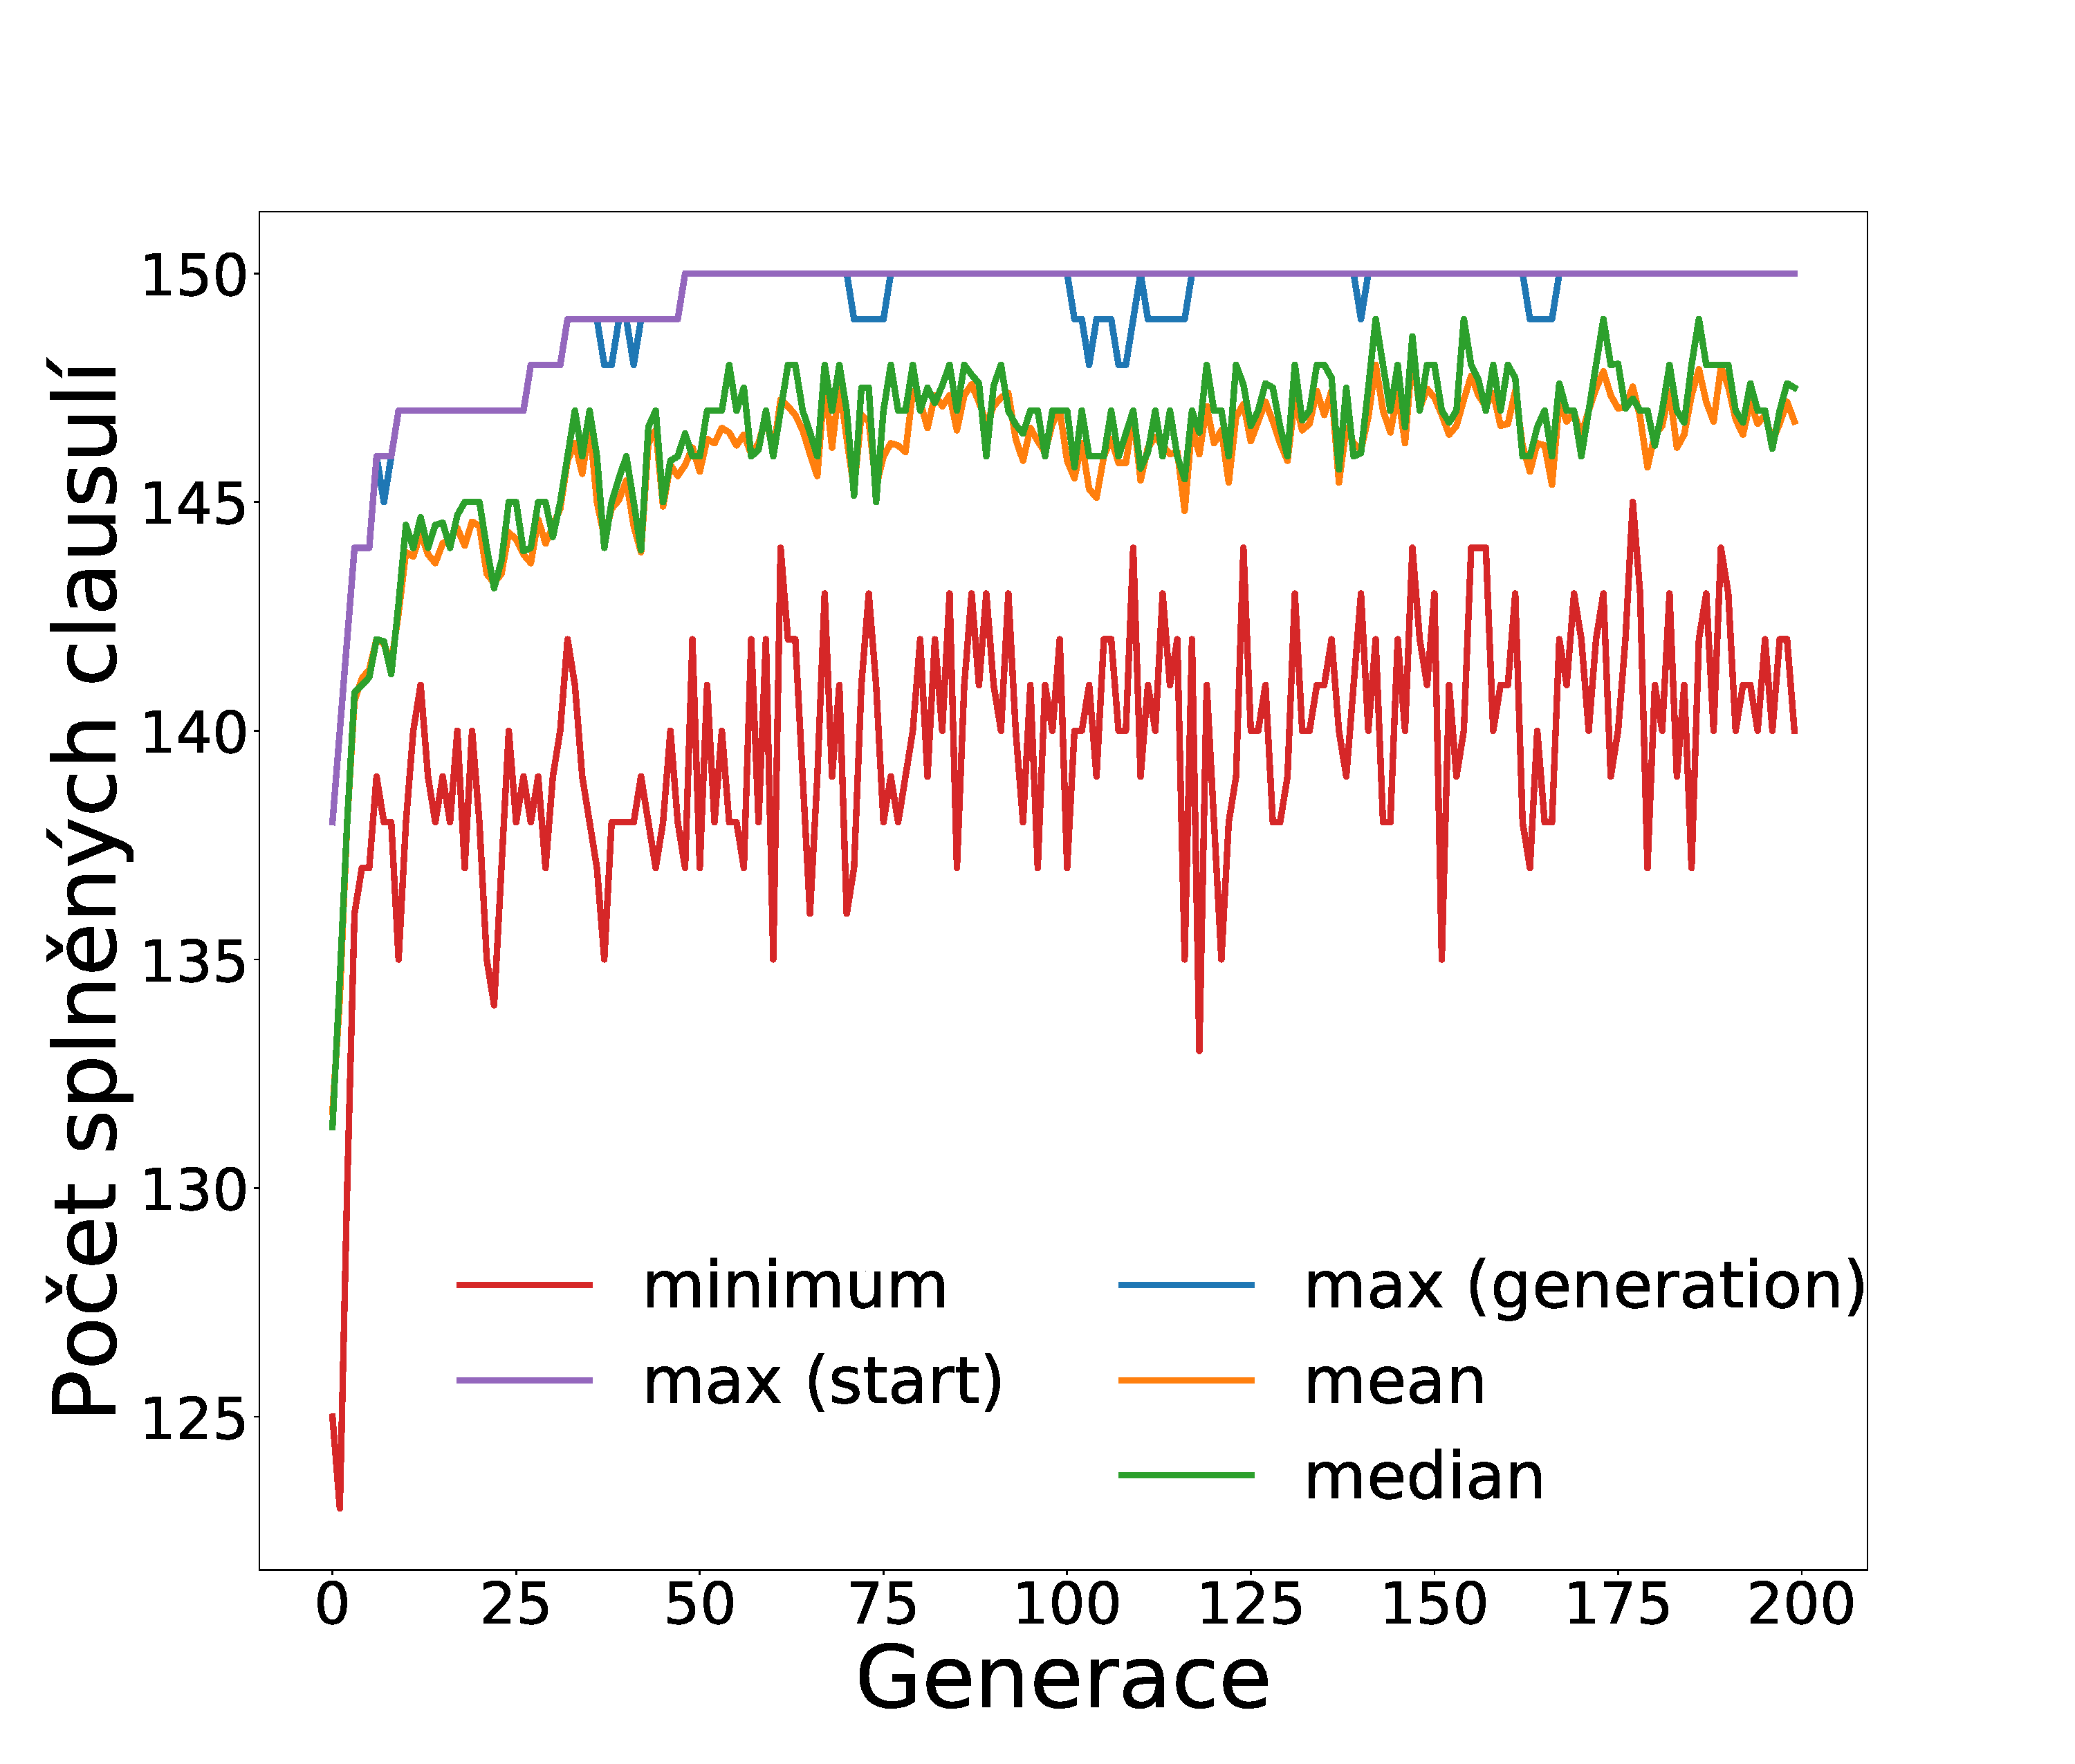
\includegraphics[width=\textwidth]{img/runC.pdf} 
    \end{minipage}
    \begin{minipage}[c]{0.48\textwidth}
        \centering 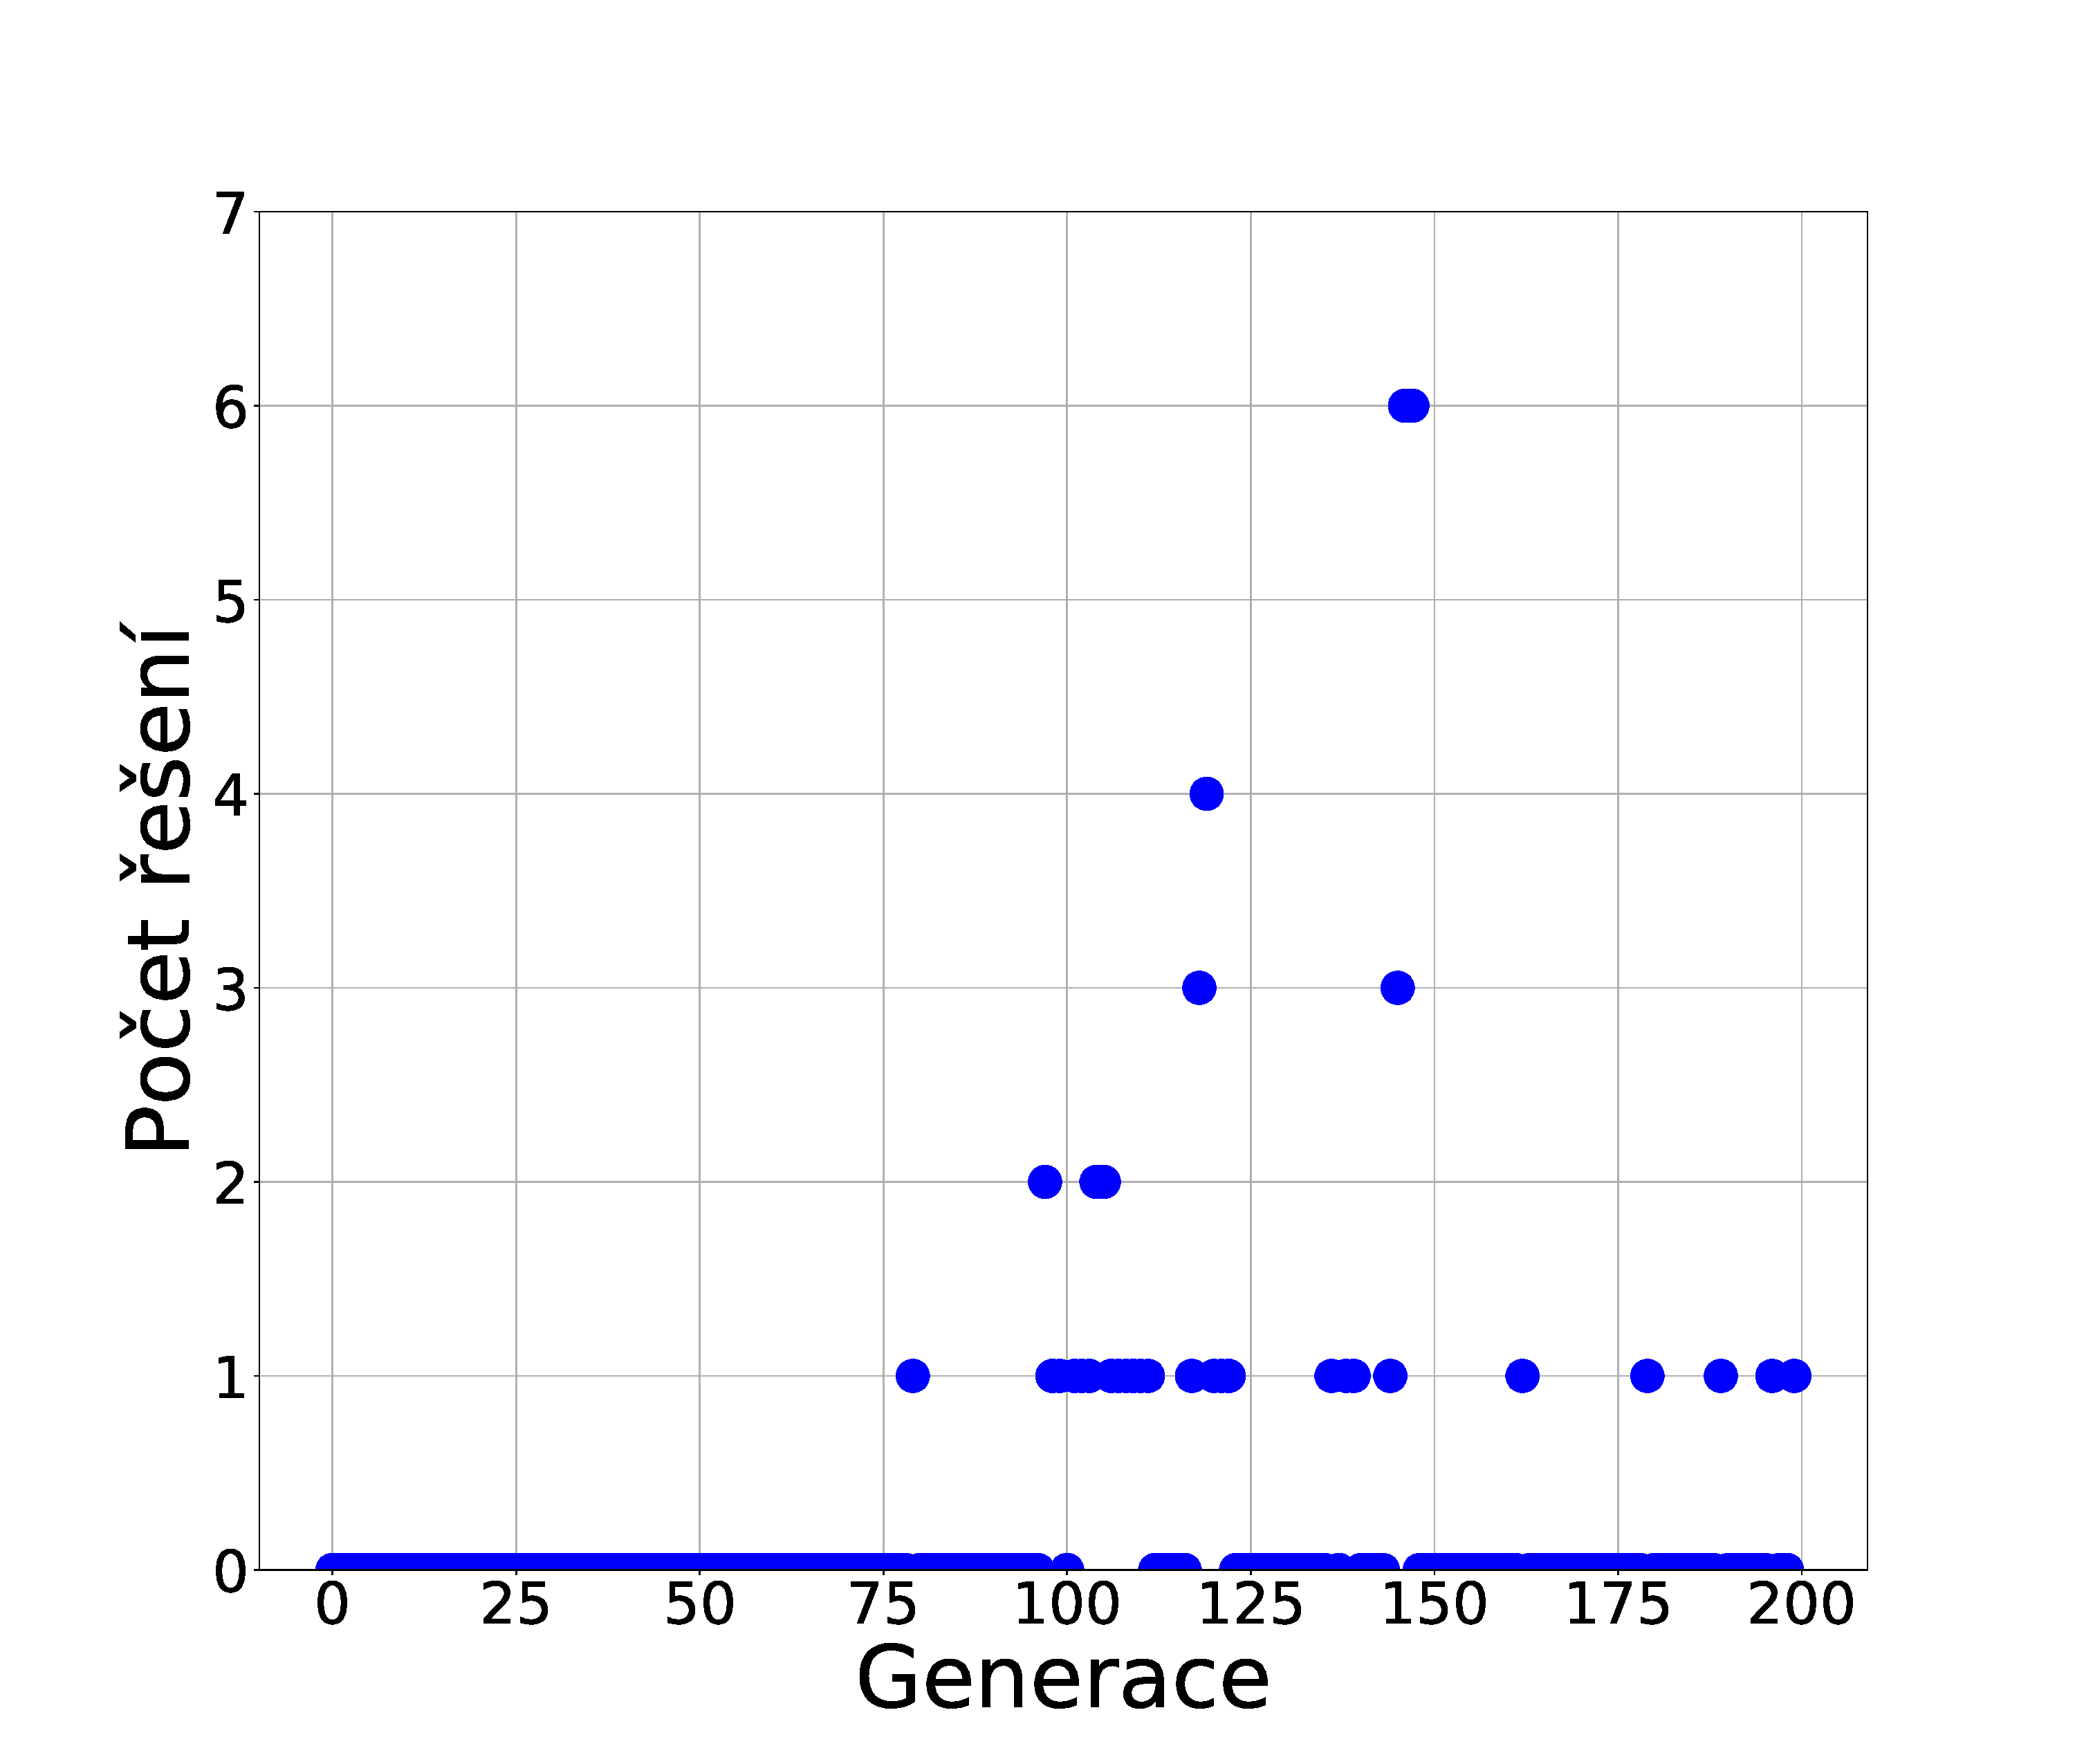
\includegraphics[width=\textwidth]{img/runS.pdf} 
    \end{minipage}
    \\
    \begin{minipage}[c]{0.48\textwidth}
        \centering 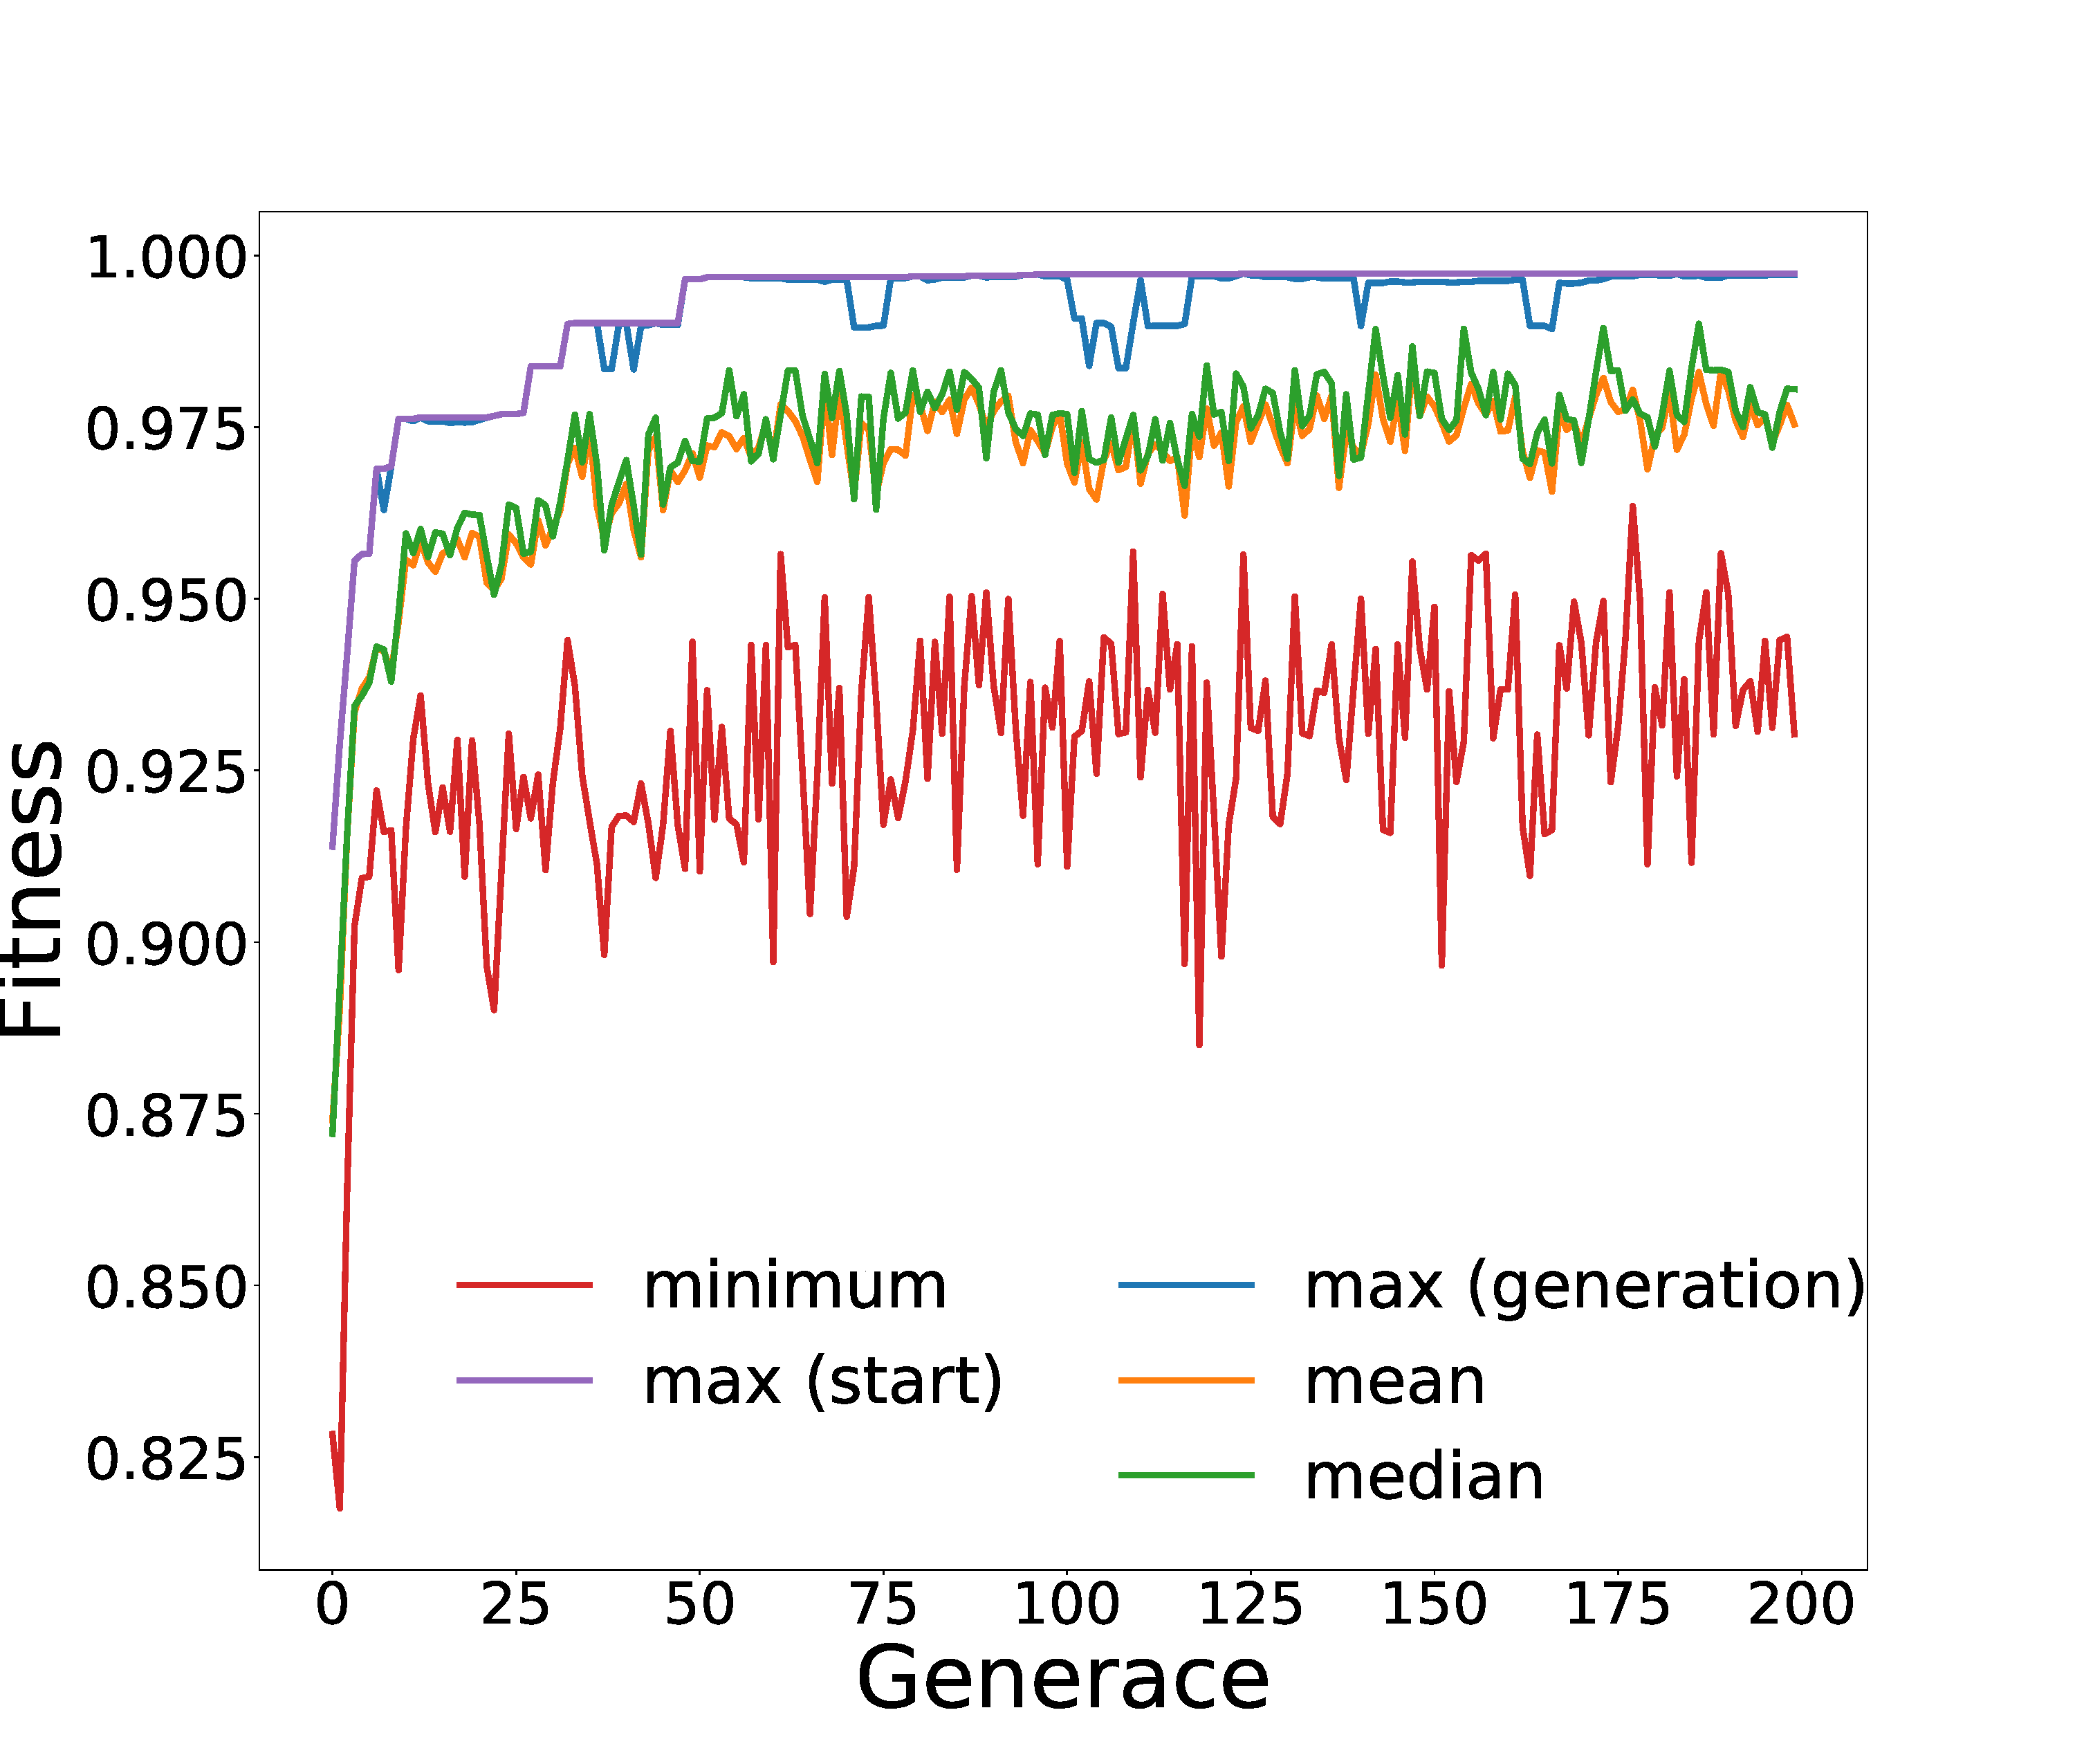
\includegraphics[width=\textwidth]{img/runG.pdf} 
    \end{minipage}
    \begin{minipage}[c]{0.48\textwidth}
        \centering 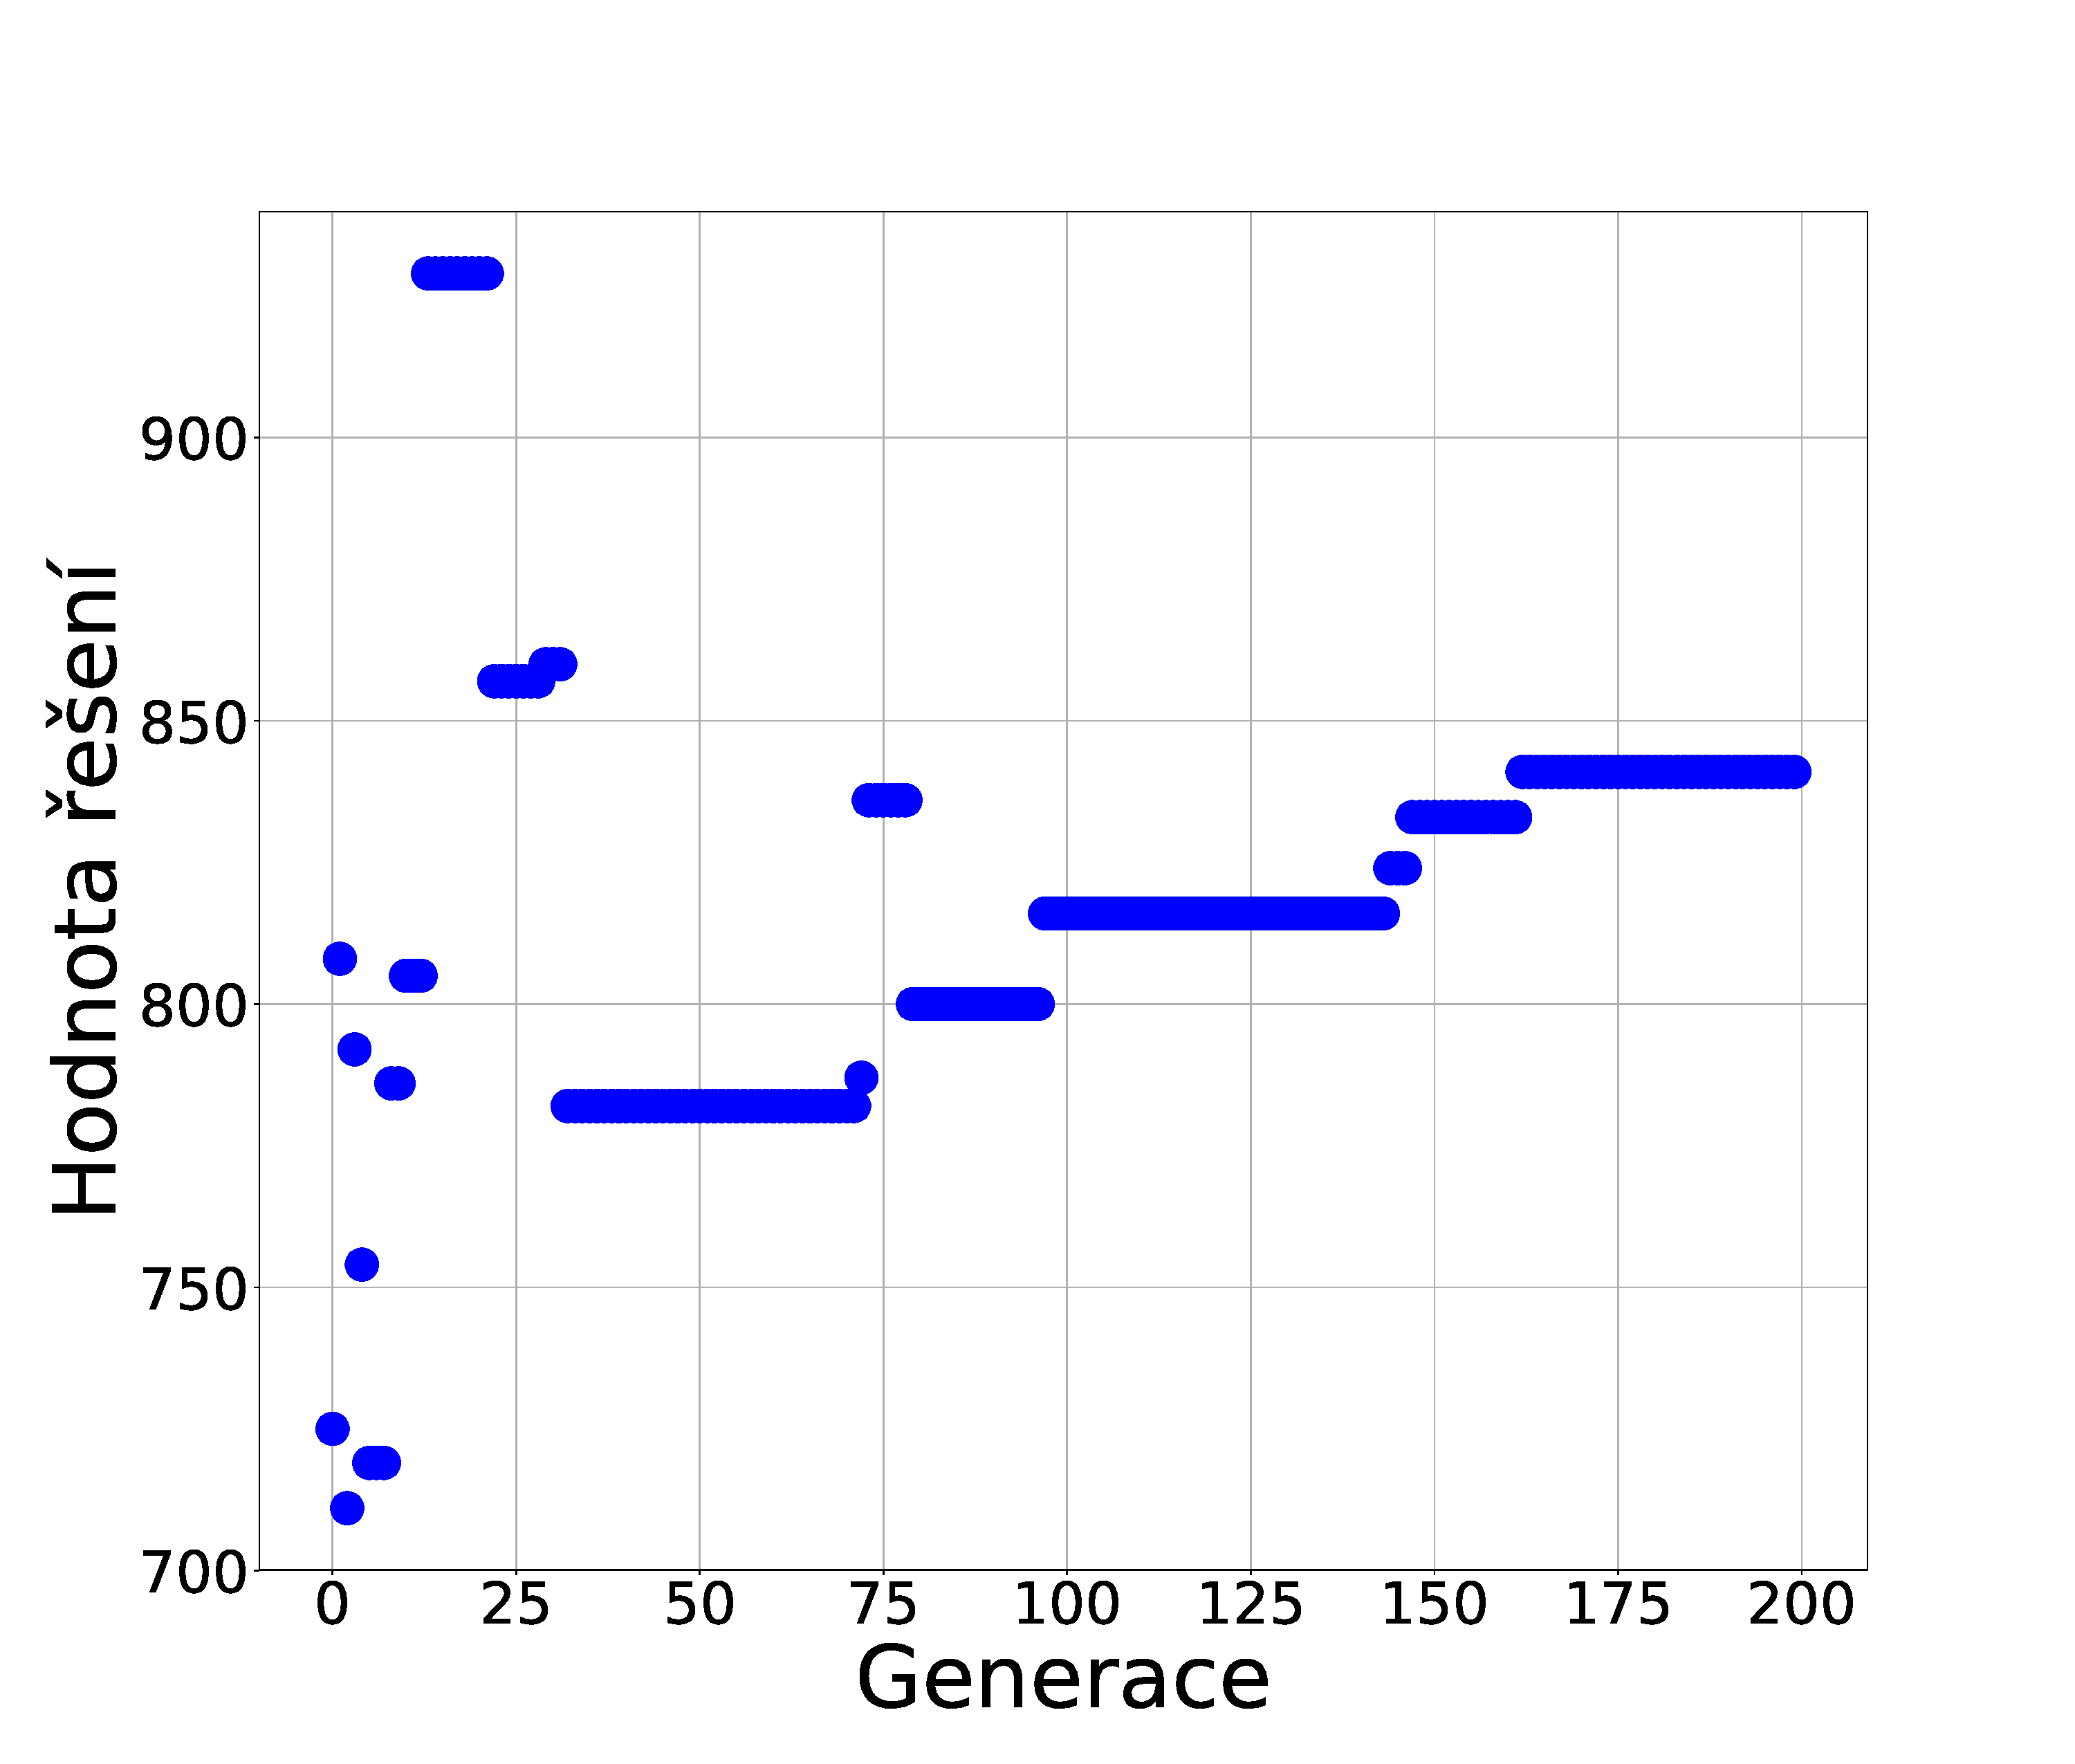
\includegraphics[width=\textwidth]{img/runW.pdf} 
    \end{minipage}
   \caption{Na obrázcích jsou grafy generované při běhu algoritmu. Vlevo nahoře je graf, kde je v rámci generací zobrazen počet splněných klauzulí. Pod ním je stejný graf pouze s rozdílem, že zde jsou zobrazeny hodnoty fitness funkce. Graf vpravo nahoře ukazuje počet řešení v~populaci v~rámci generačního cyklu. Na grafu pod ním je vývoj maximální dosažené váhy proměných v~rámci generačního cyklu.}\label{fig:normalrun}
\end{figure} 

\section{Experimenty}\label{kap:experiments}

\begin{figure}
	\centering
    \begin{minipage}[c]{0.325\textwidth}
        \centering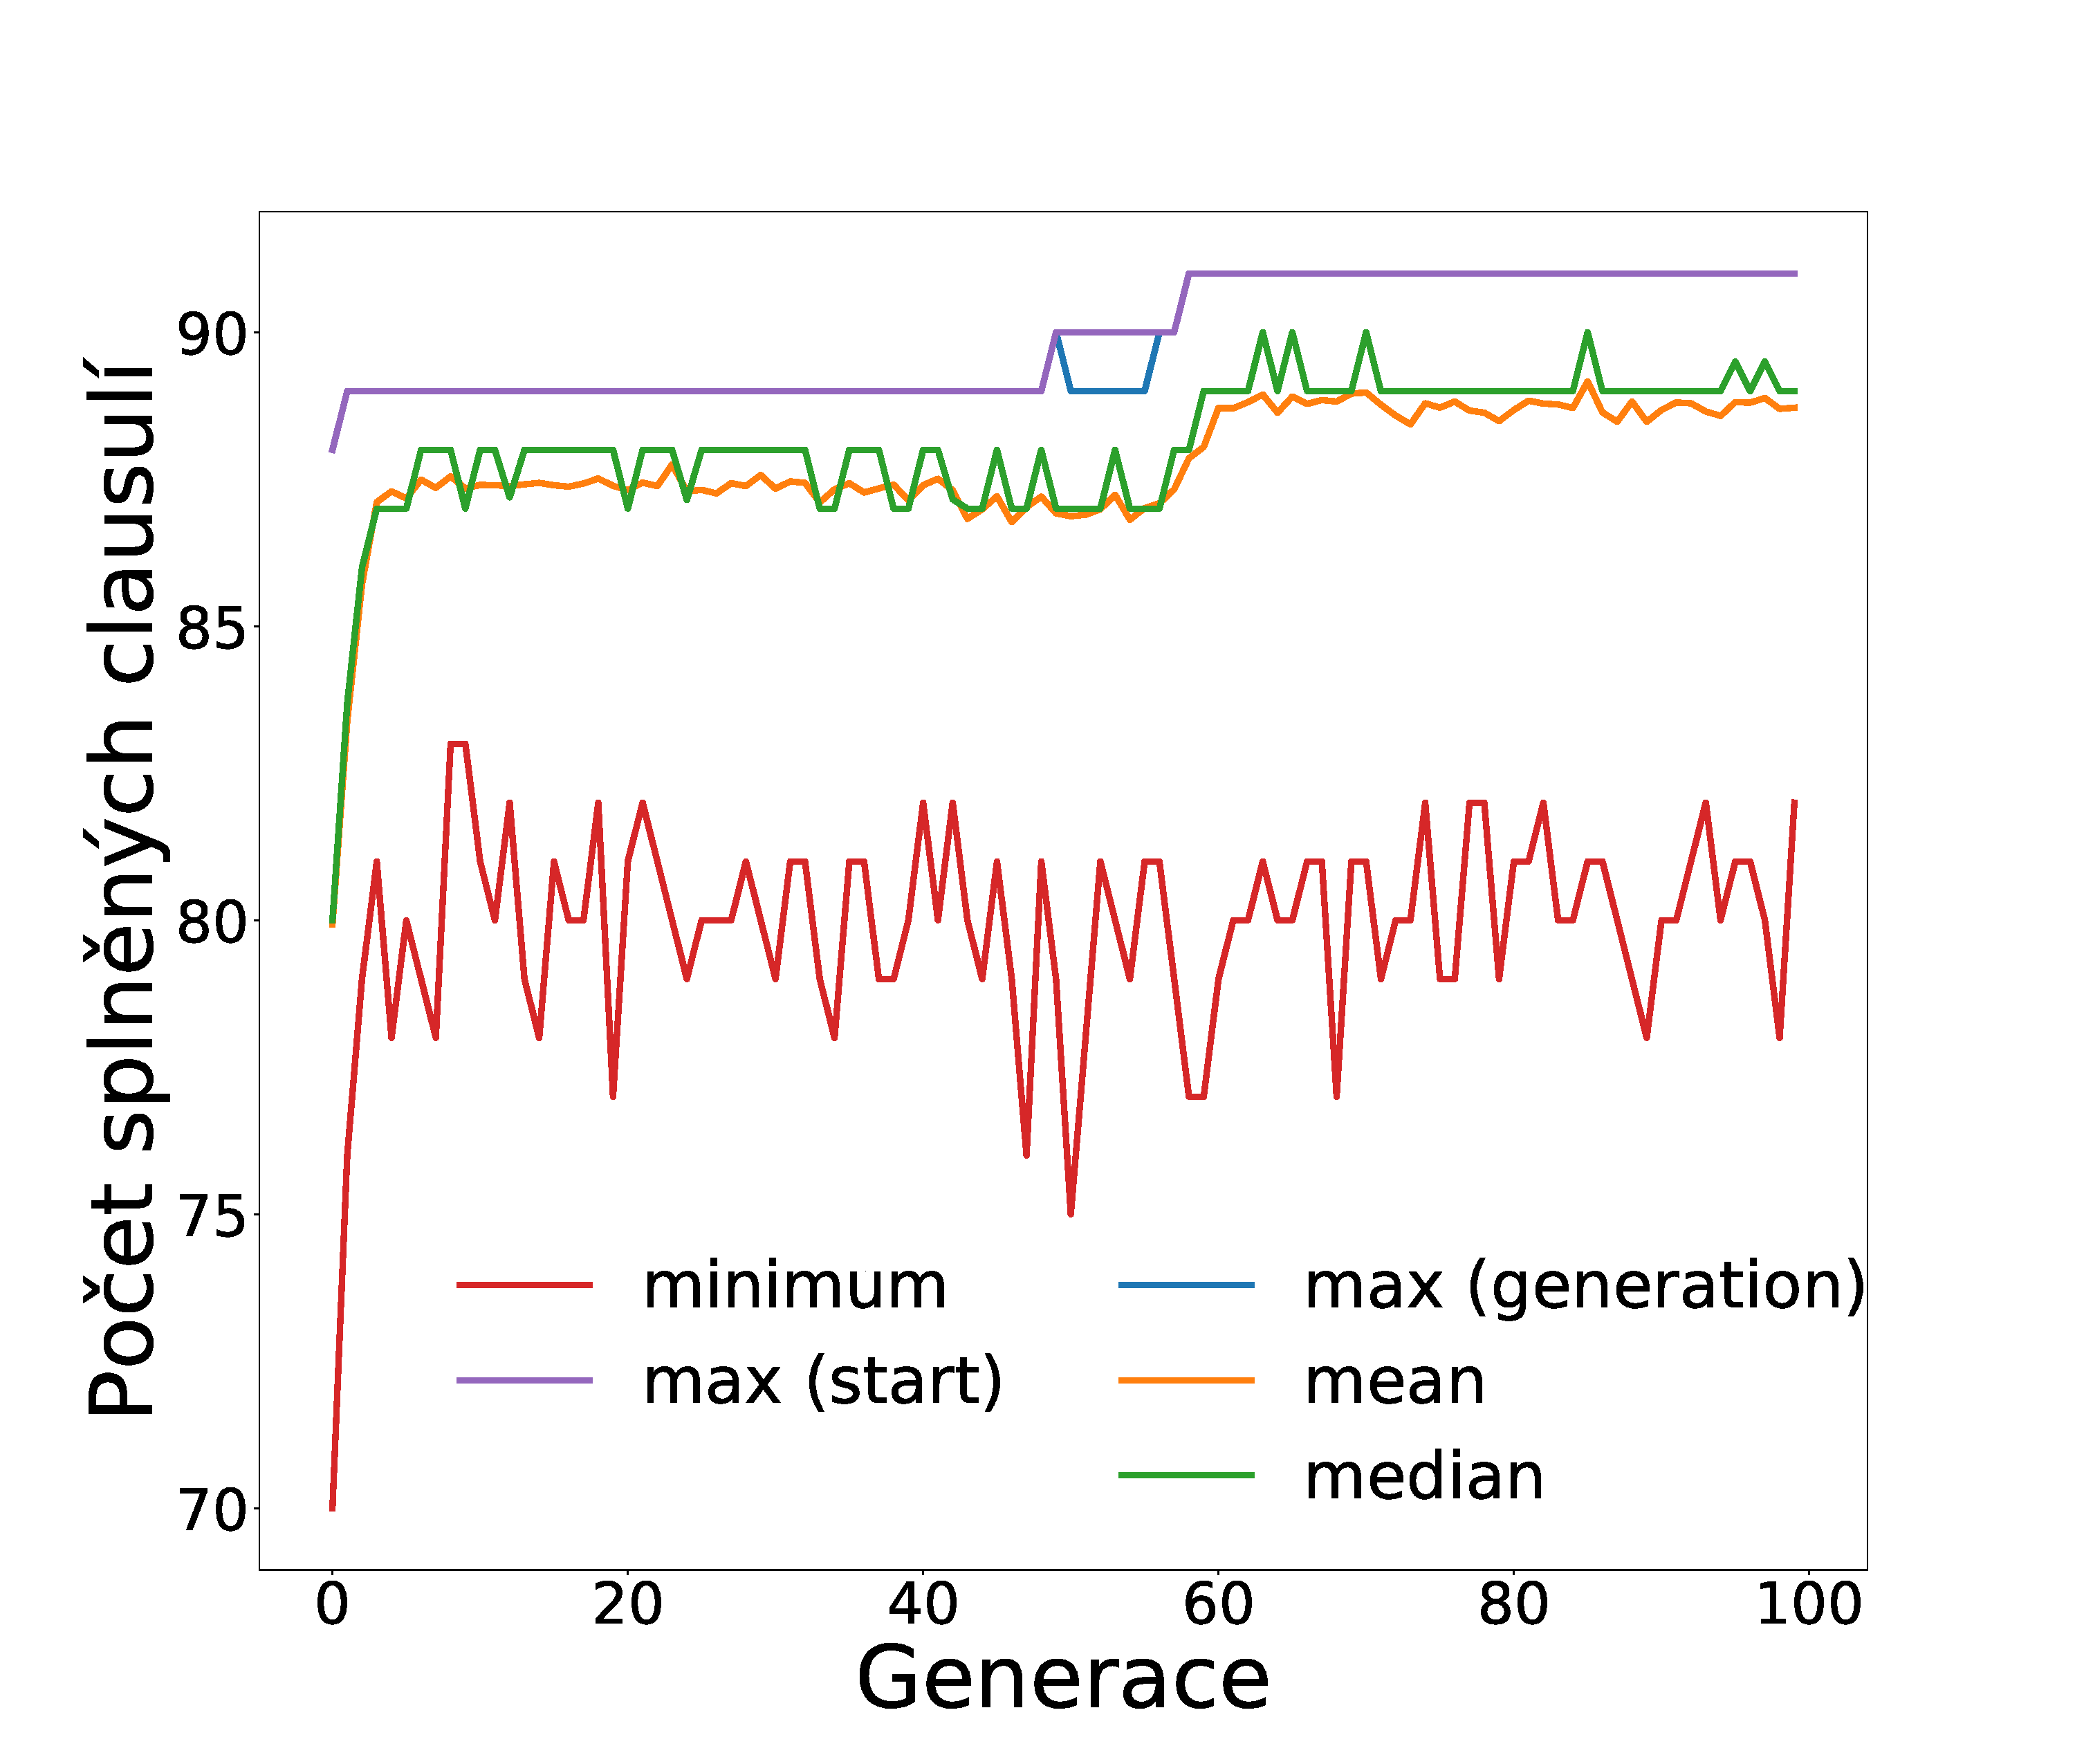
\includegraphics[width=\textwidth]{img/badC.pdf} 
    \end{minipage}
    \begin{minipage}[c]{0.325\textwidth}
        \centering 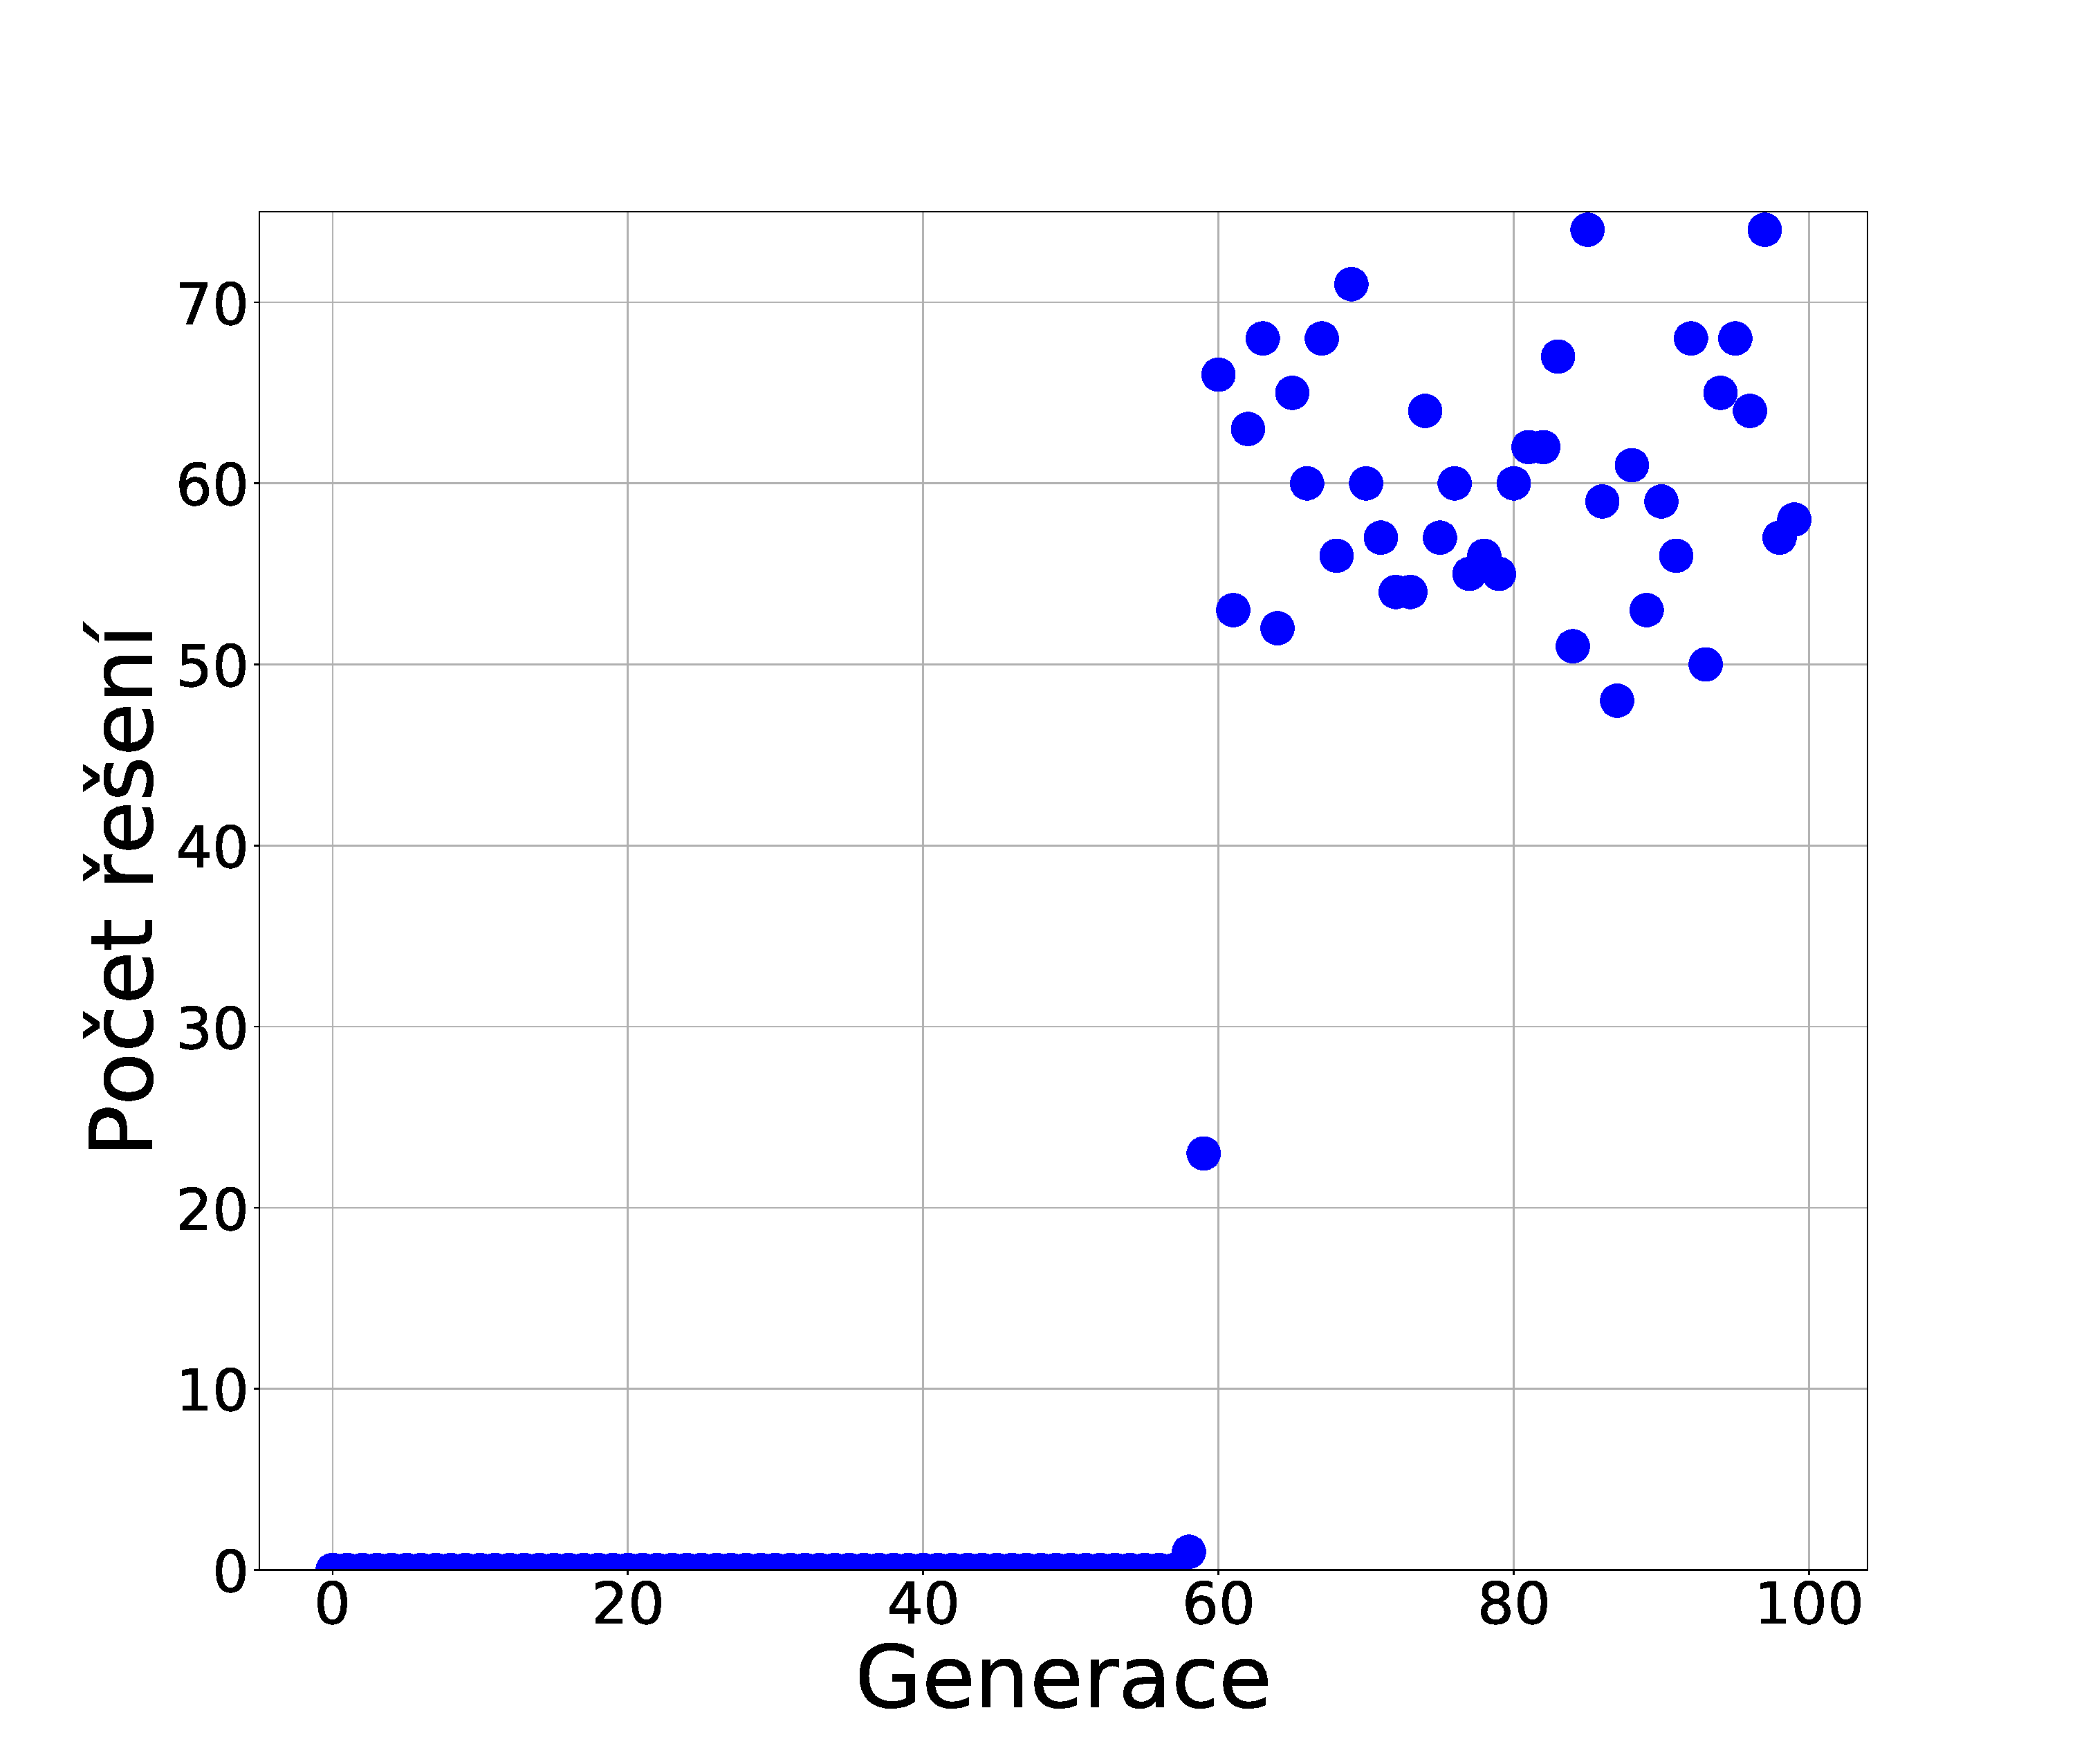
\includegraphics[width=\textwidth]{img/badS.pdf} 
    \end{minipage}
    \begin{minipage}[c]{0.325\textwidth}
        \centering 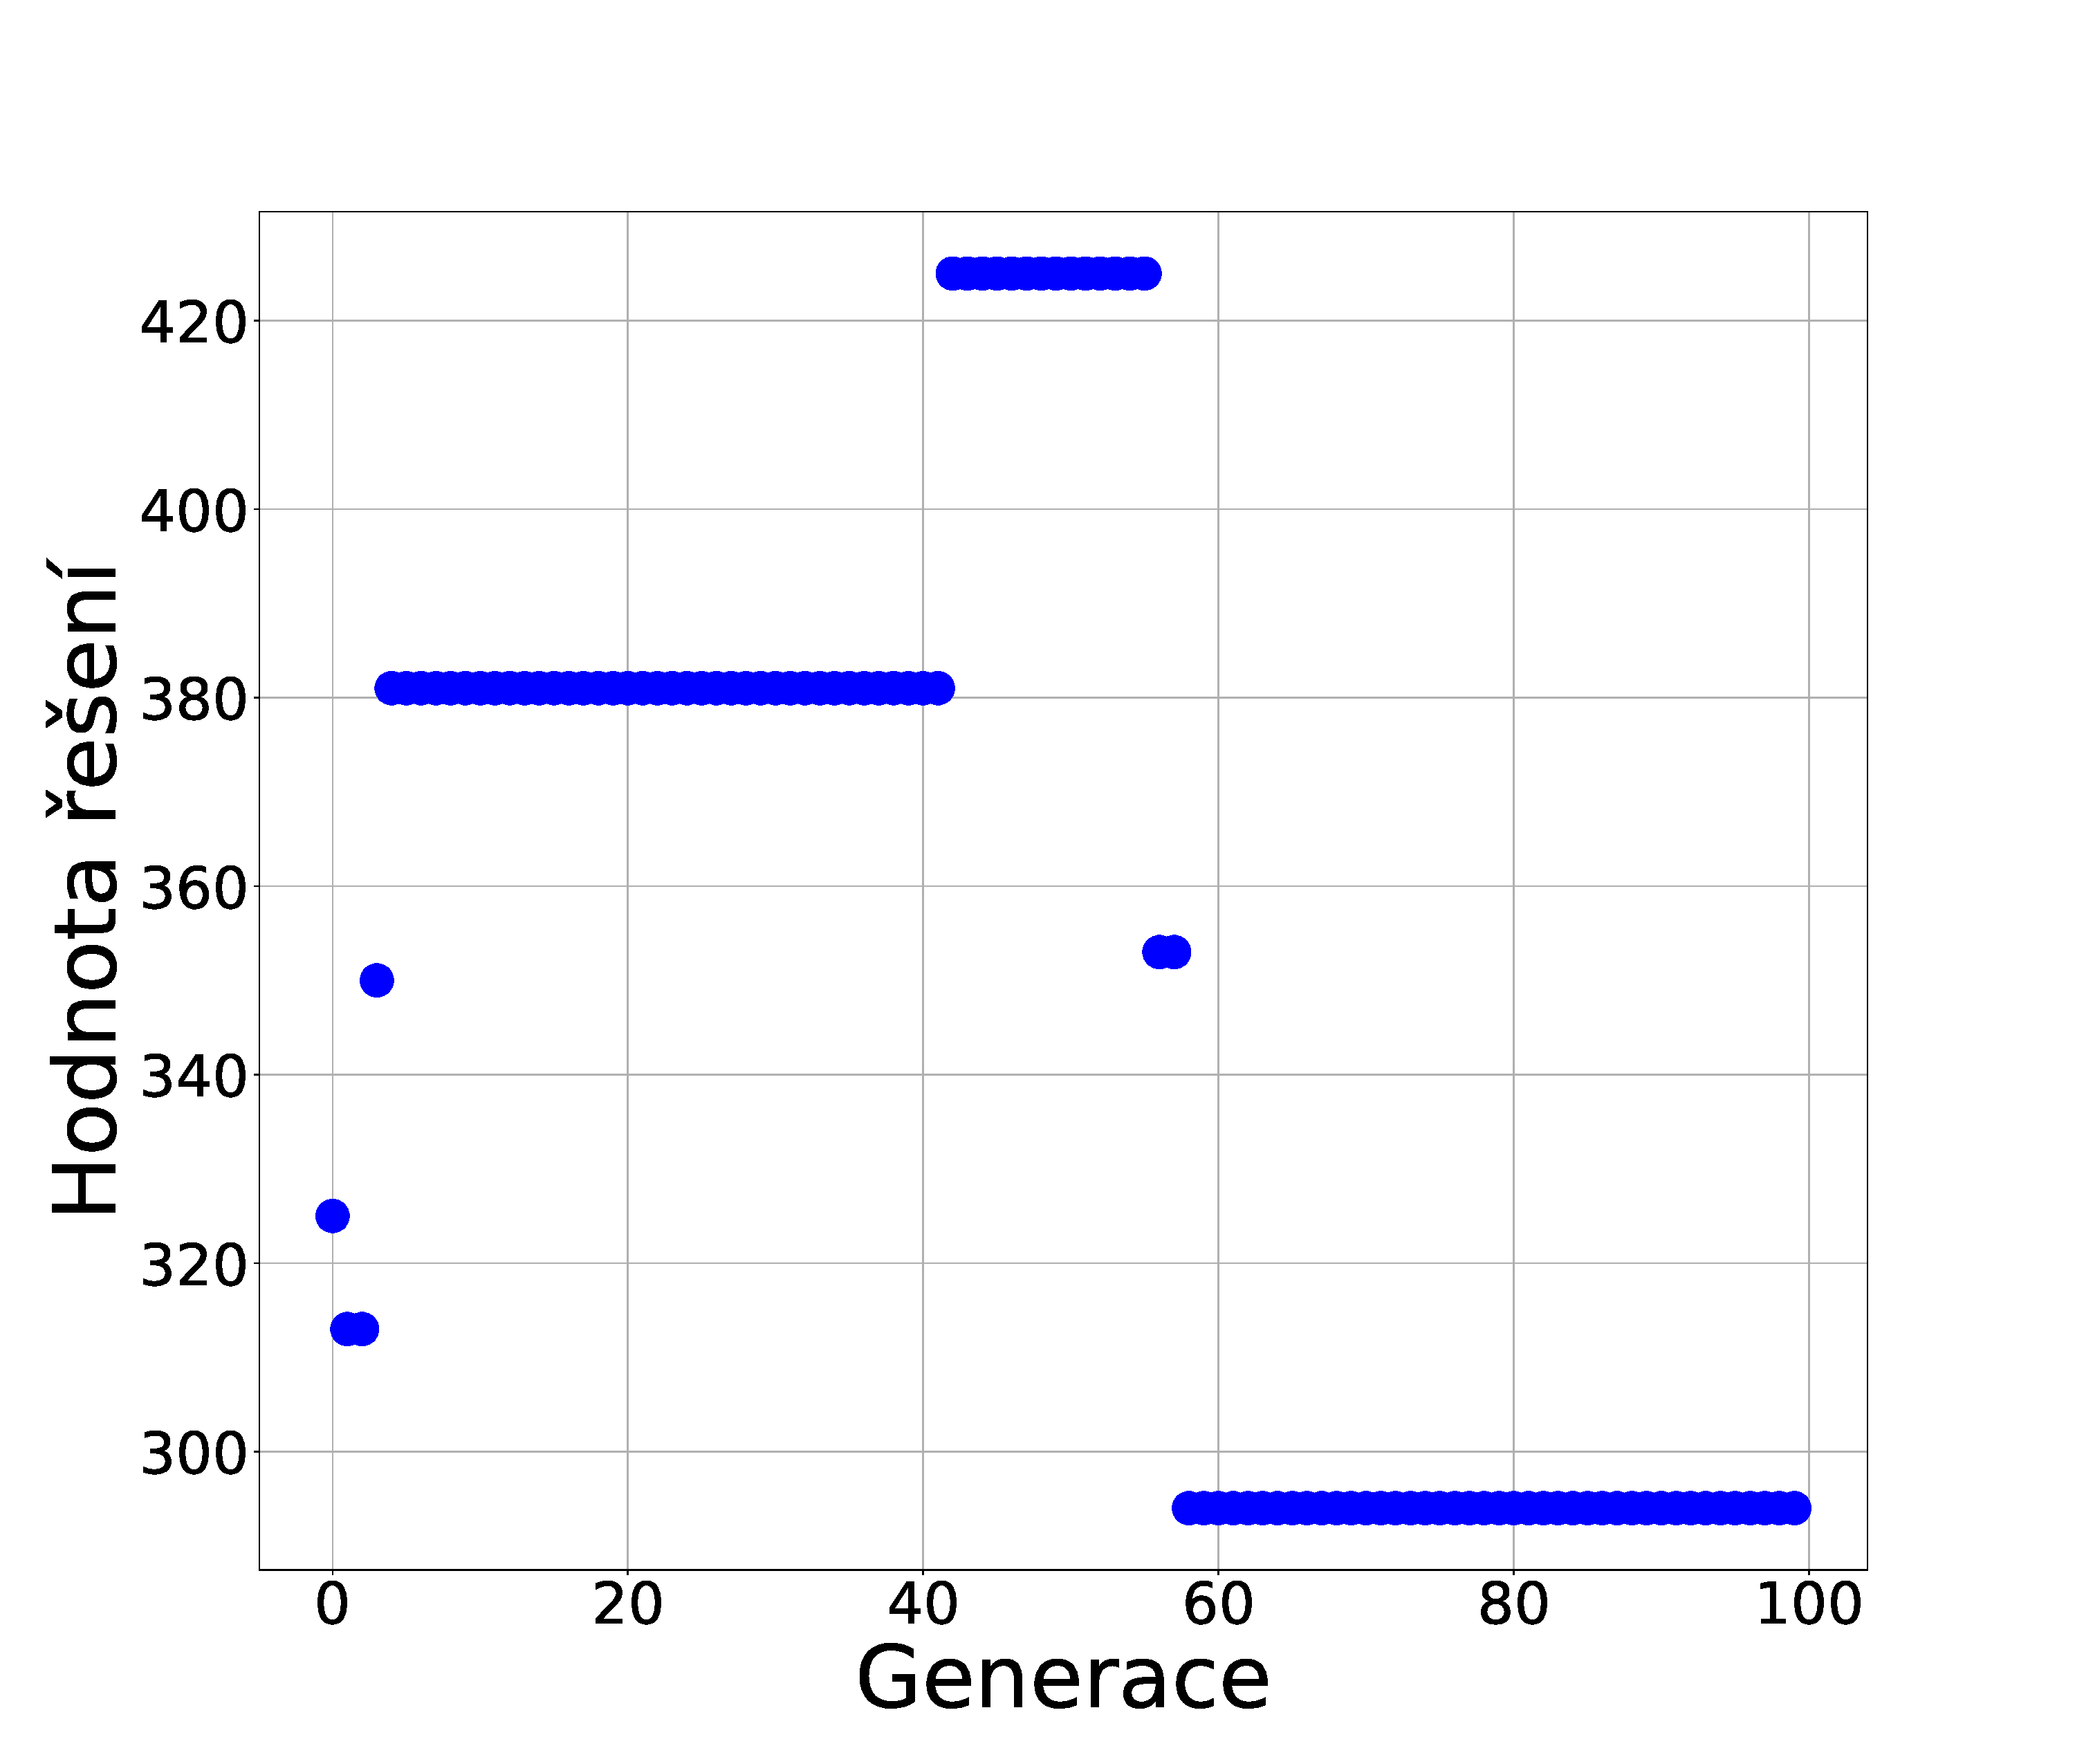
\includegraphics[width=\textwidth]{img/badW.pdf} 
    \end{minipage}
    \\
   \caption{Na obrázcích je ukázán ne úplně ideální průběh. Na levém obrázku počet splněných klauzulí, uprostřed počet řešení v populaci a na pravém váha nejlepšího řešení.}\label{fig:badrun}
\end{figure} 


V experimetech prozkoumám závislost genetického algoritmu na parametrech jako jsou počet generací, velikost populace, hodnota mutace, pravděpodobnost křížení a selekční tlak. Vždy se pokusím testovat jeden parametr a ostatní zafixuji, aby bylo možné měřit vliv tohoto parametru na průběh řešení. Zafixované hodnoty mají hodnotu z ukázky nastavení níže a pro hodnotu mutace je hodnota 0,05.

V rámci běhu algoritmu program vytváří grafy o běhu a jsou zaznámenávány statistiky do csv souboru. Na obrázku \ref{fig:normalrun} jsem uvedl příklad normálního a úspěšněho běhu iterativní heuristiky. Je také vidět, že hodnota fitness funkce a počet splněných klauzulí spolu velice korelují, což bylo předpokládáno již při sestavení vzorce pro výpočet fitness funkce. Proto v následujících experimentech budu vždy uvádět jen jeden z těchto dvou grafů, protože jsou téměř totožné. Grafy na obrázku \ref{fig:normalrun} jsou vygenerovány s nastaveními níže, kde mutace je 0,05, tedy první hodnota ze seznamu. Konfigurační souborem ukaázaným níže, lze tedy řídit chování programu a algoritmu a tento soubor je nutné zadat při spuštění.

V experimentech jsem tedy měřil především dosaženou hodnotu fitness funkce a procento spl\-něných klauzulí. Na těchto hodnotách budu také především testovat chování algoitmu na změnu parametrů za cílem nalezení nastavení, které bude při řešení problému nejúspěšnější. 

\begin{labeling}{alligator}
\item[RUN:] 
\begin{labeling}{alligator}
\item[] 
\item[out:] ./out/t
\item[in:] ./instCtV
\end{labeling}
\item[GA:]
\begin{labeling}{alligator}
\item[] 
\item[generationcount:] 200
\item[generationsize:] 200
\item[mutation:] 0,05 0,21 0,05
\item[crossover:] 0,7
\item[selection:] 0,1
\item[selection\_add:] 2
\item[elitism:] 1
\item[fitness:] 0,99
\end{labeling}  
\end{labeling}
\pagestyle{plain}

Na obrázku \ref{fig:normalrun} je ještě patrný vysoký koeficient ve fitness funkci, kde je hlavní podmínkou splnění klauzule. Jak je patrné, tak při naležení řešení poklesla hodnota řešení, protože paramentr hodnoty nebyl tak upřednostňvaný a hodnota se opět zlepšovala v dalších generací, kdy už v řešení byly přítomna řešení. Toto je velice markantní na obrázku \ref{fig:badrun}, takto také dopadaly běhy algoritmu. Při běhu bylo nalezeno řešení, hodnota řešení prudce klesla, ale již se ji nepodařilo vylepšit. Bohužel z důvodu neznalosti optimálního řešení nedokáži posoudit, zdali náhodou toto nebylo optimální řešení, pro splnění problému SAT.

\begin{figure}
	\centering
    \begin{minipage}[c]{0.48\textwidth}
        \centering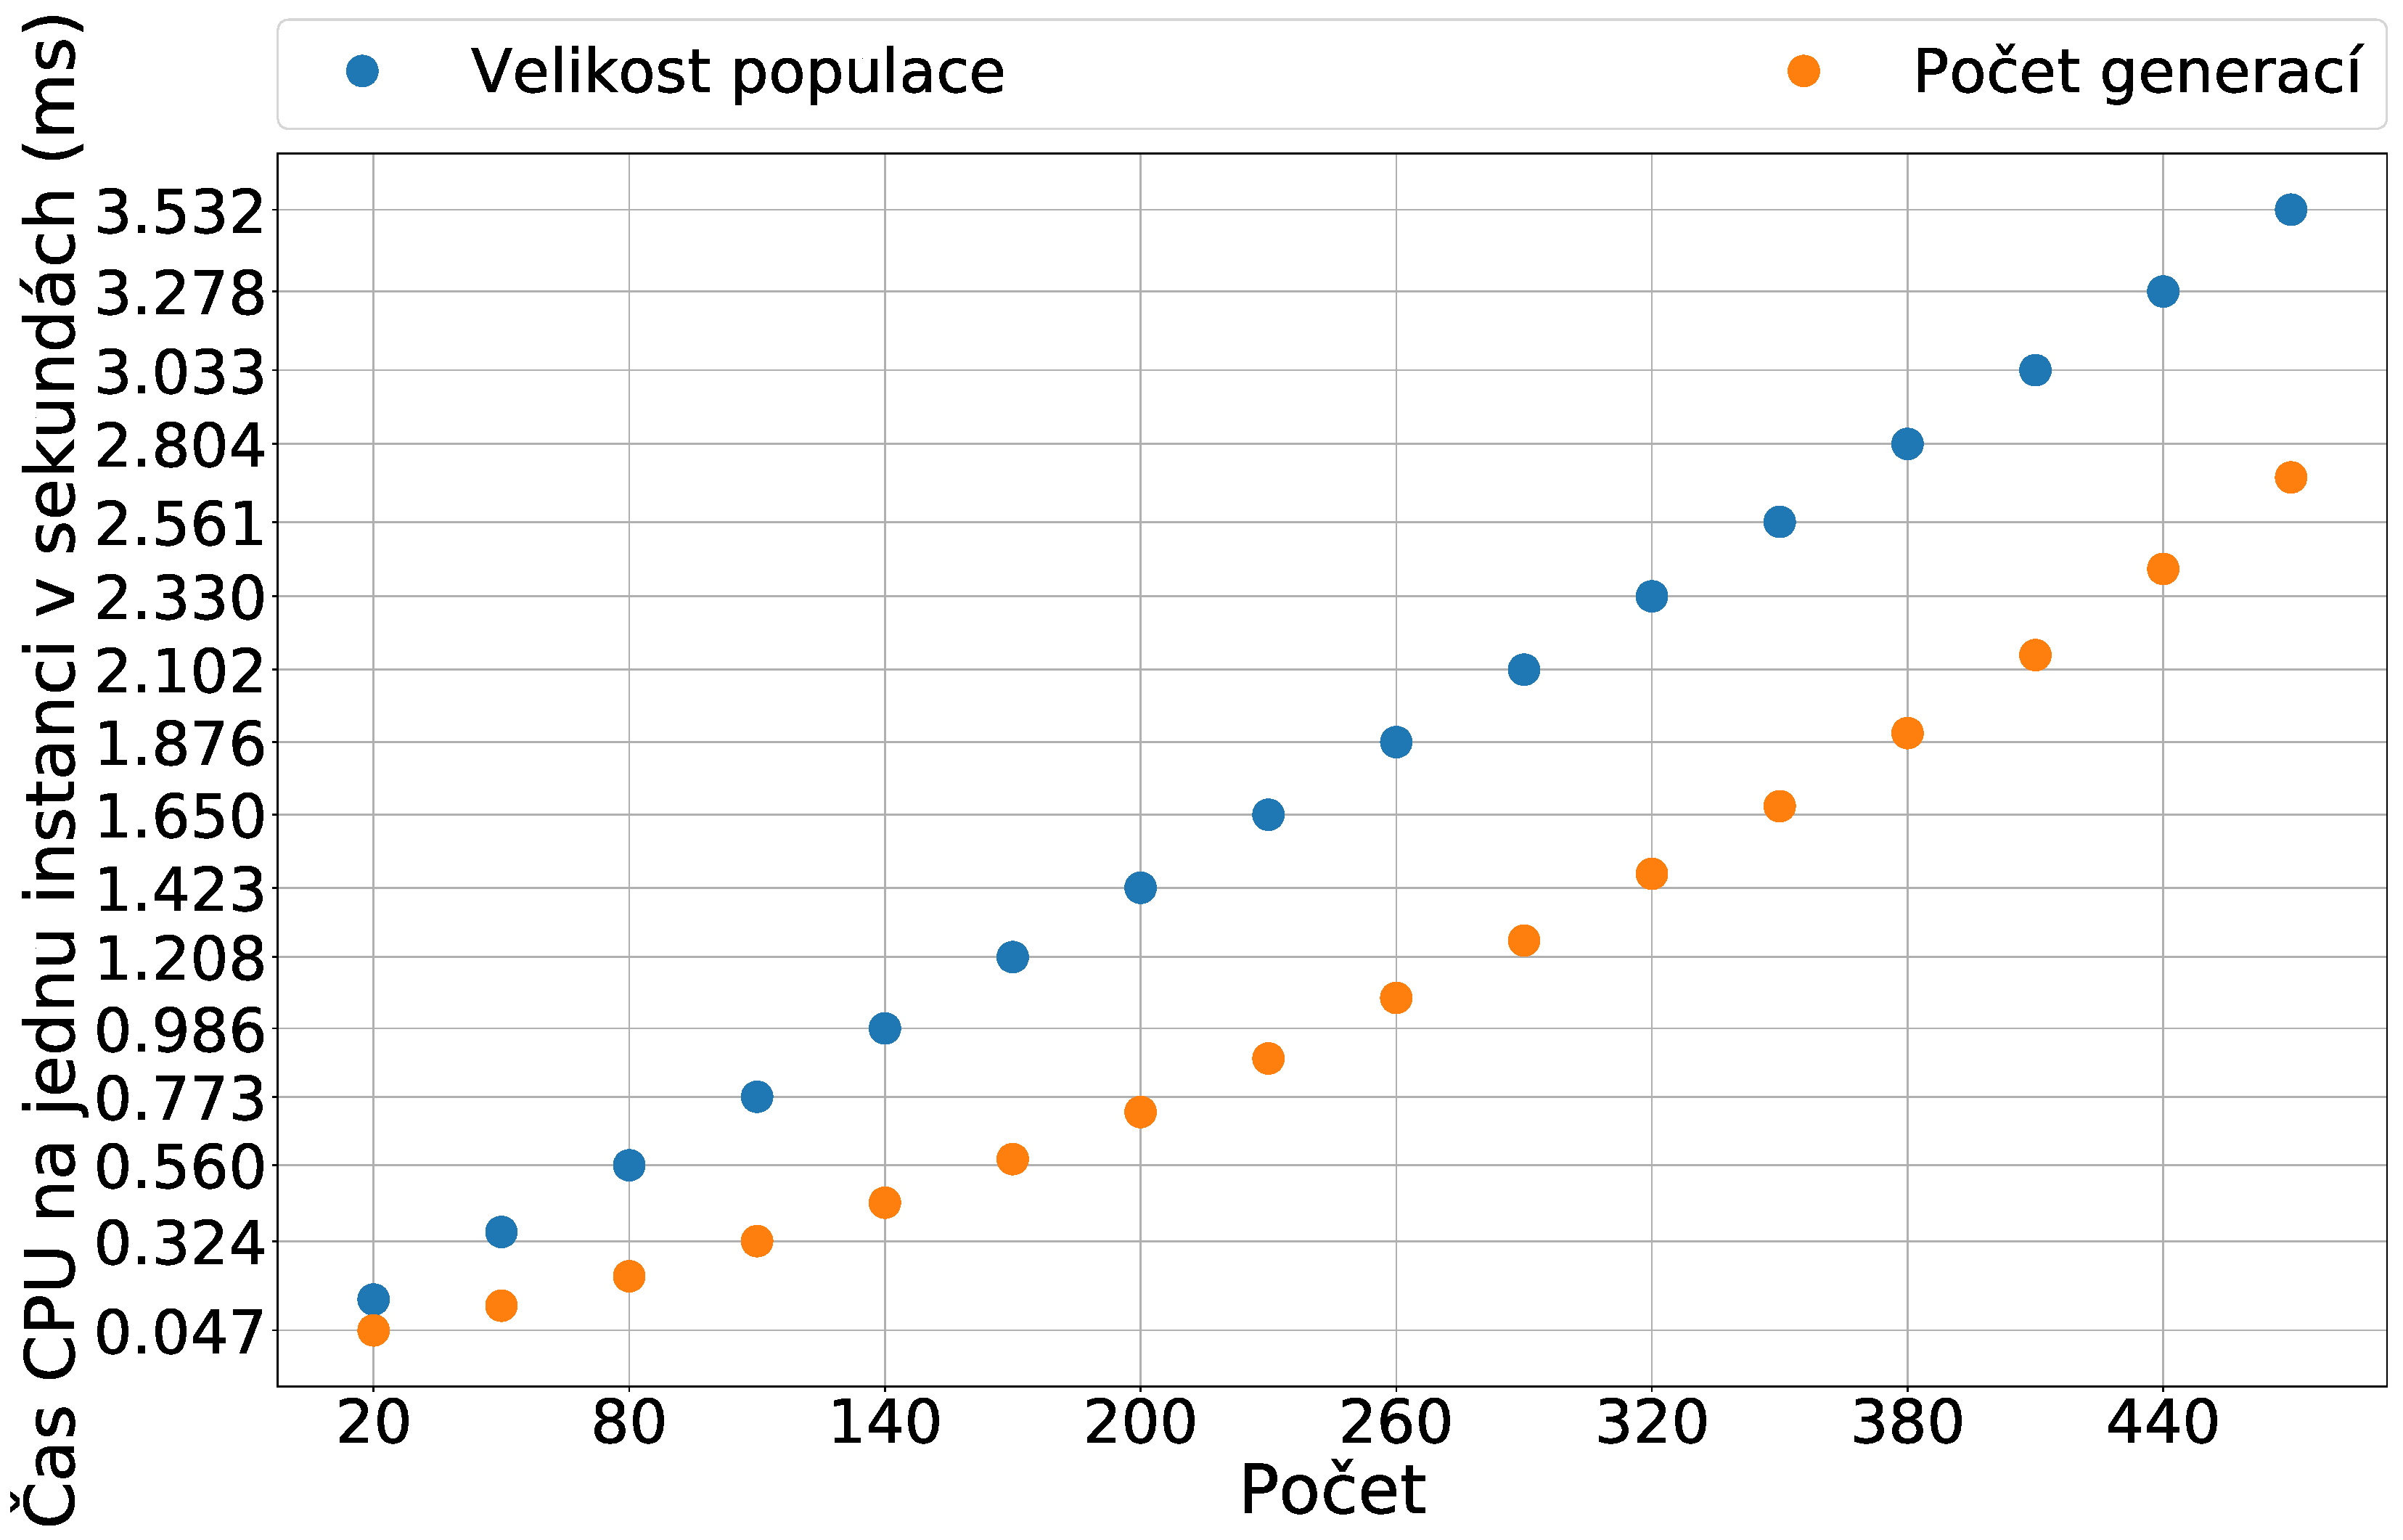
\includegraphics[width=\textwidth]{img/time_gen_cnt_sz.pdf} 
    \end{minipage}
    \begin{minipage}[c]{0.48\textwidth}
        \centering 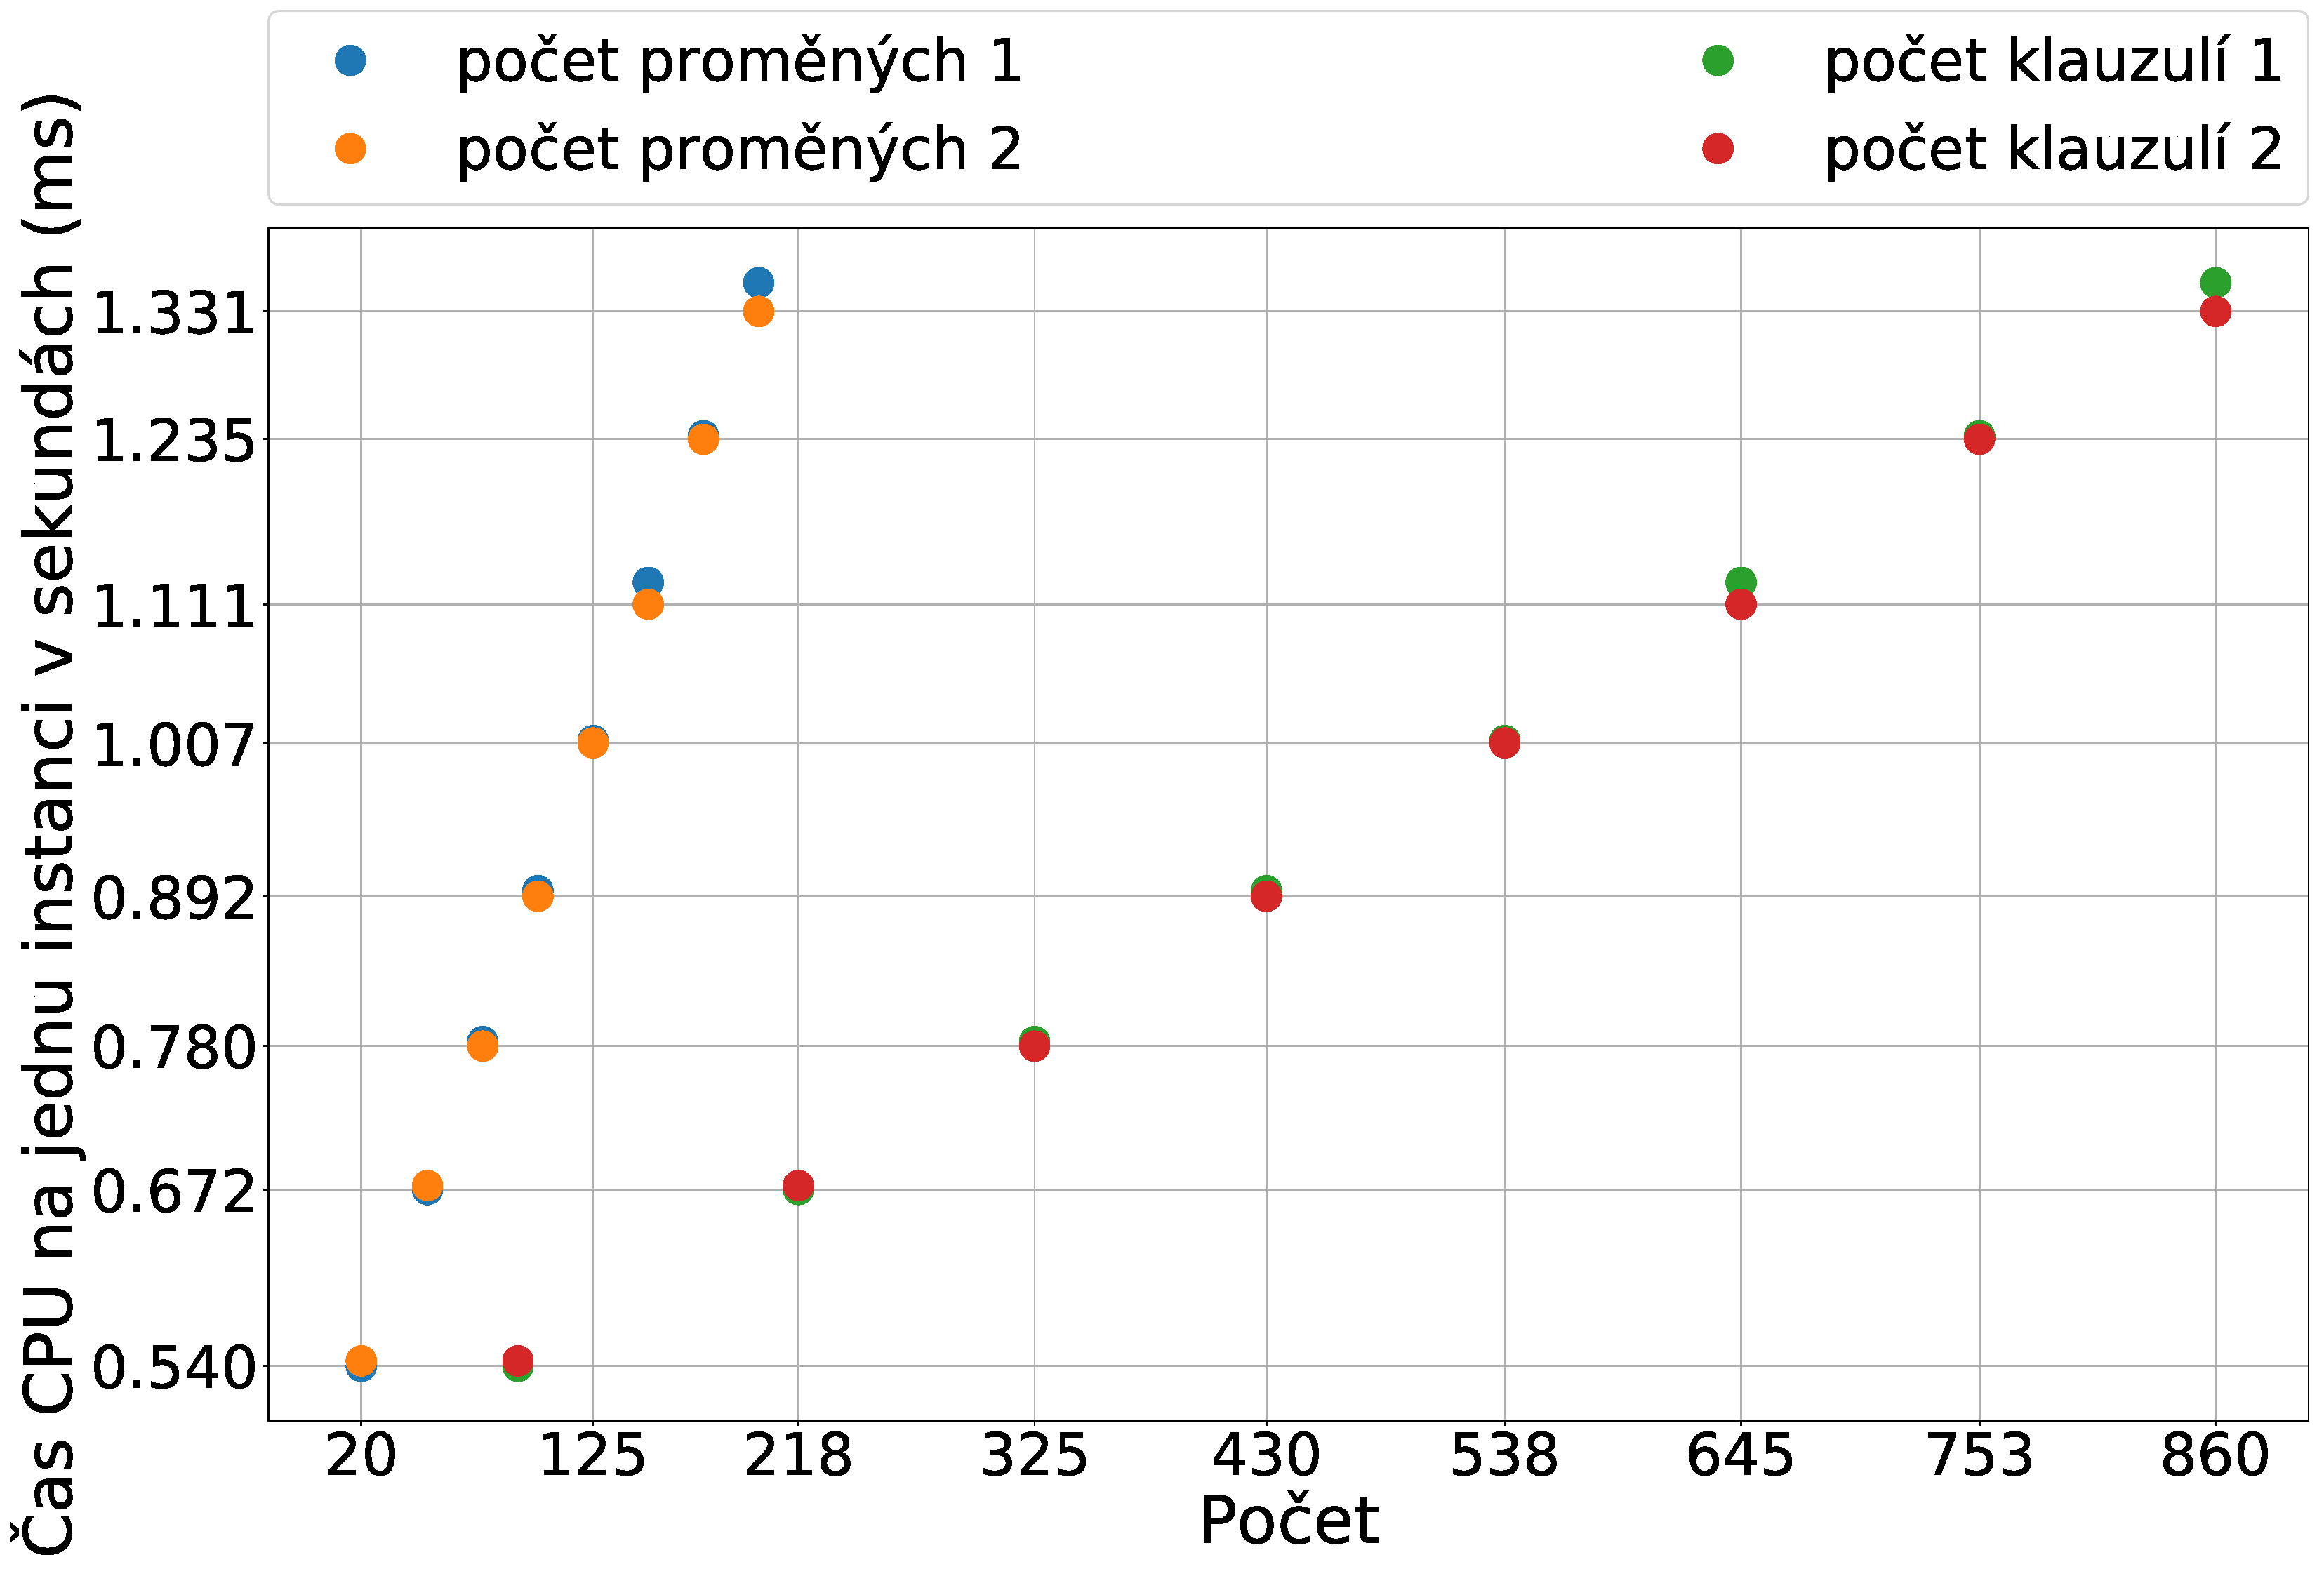
\includegraphics[width=\textwidth]{img/time_n_var_cla.pdf} 
    \end{minipage}
    \\
   \caption{Na grafech jsou vidět časové náročnosti. Na levém grafu je zobrazena časová náročnost na velikosti populace a počtu generací. Na pravém grafu je zobrazena časová závislost na počtu proměných a počtu klauzulí v problému.}\label{fig:time}
\end{figure} 
\subsection{Závislosti některý parametrů instancí a algoritmu na výpočetním čase}
Závislosti na čase, které předpokládám jsou, že na počtu generací a počtu proměných bude algoritmus závislý lineárně. Podle naprogramovanho řešení by měl být algoritmus závislý lineárně i na počtu proměných a počtu klauzulí. Počet klauzulí by však měl běhy ovlivnit méně. 

Předpoklady se potvrdili a výsledky z měření je možné vidět na obrázku \ref{fig:time}. Závislost na počtu jedicnů v populaci je lineární jak je patrné. Závislost počtu generační cyklů se úplně lineární nejeví, ale v případě tohoto měření je to způsobeno narustající velikostí turnaje s každou generací pro zesílení selekčního tlaku, který jsem se rozhodl použít v základním nastavení. Závislost na počtu proměných a počtu klauzulí je také lineární avšak s velmi rozdílným koeficientem u přímky pokud bych se pokusil body proložit přímkou pomocí lineární regrese.


\begin{wrapfigure}{r}{0.55\textwidth}
\begin{center}
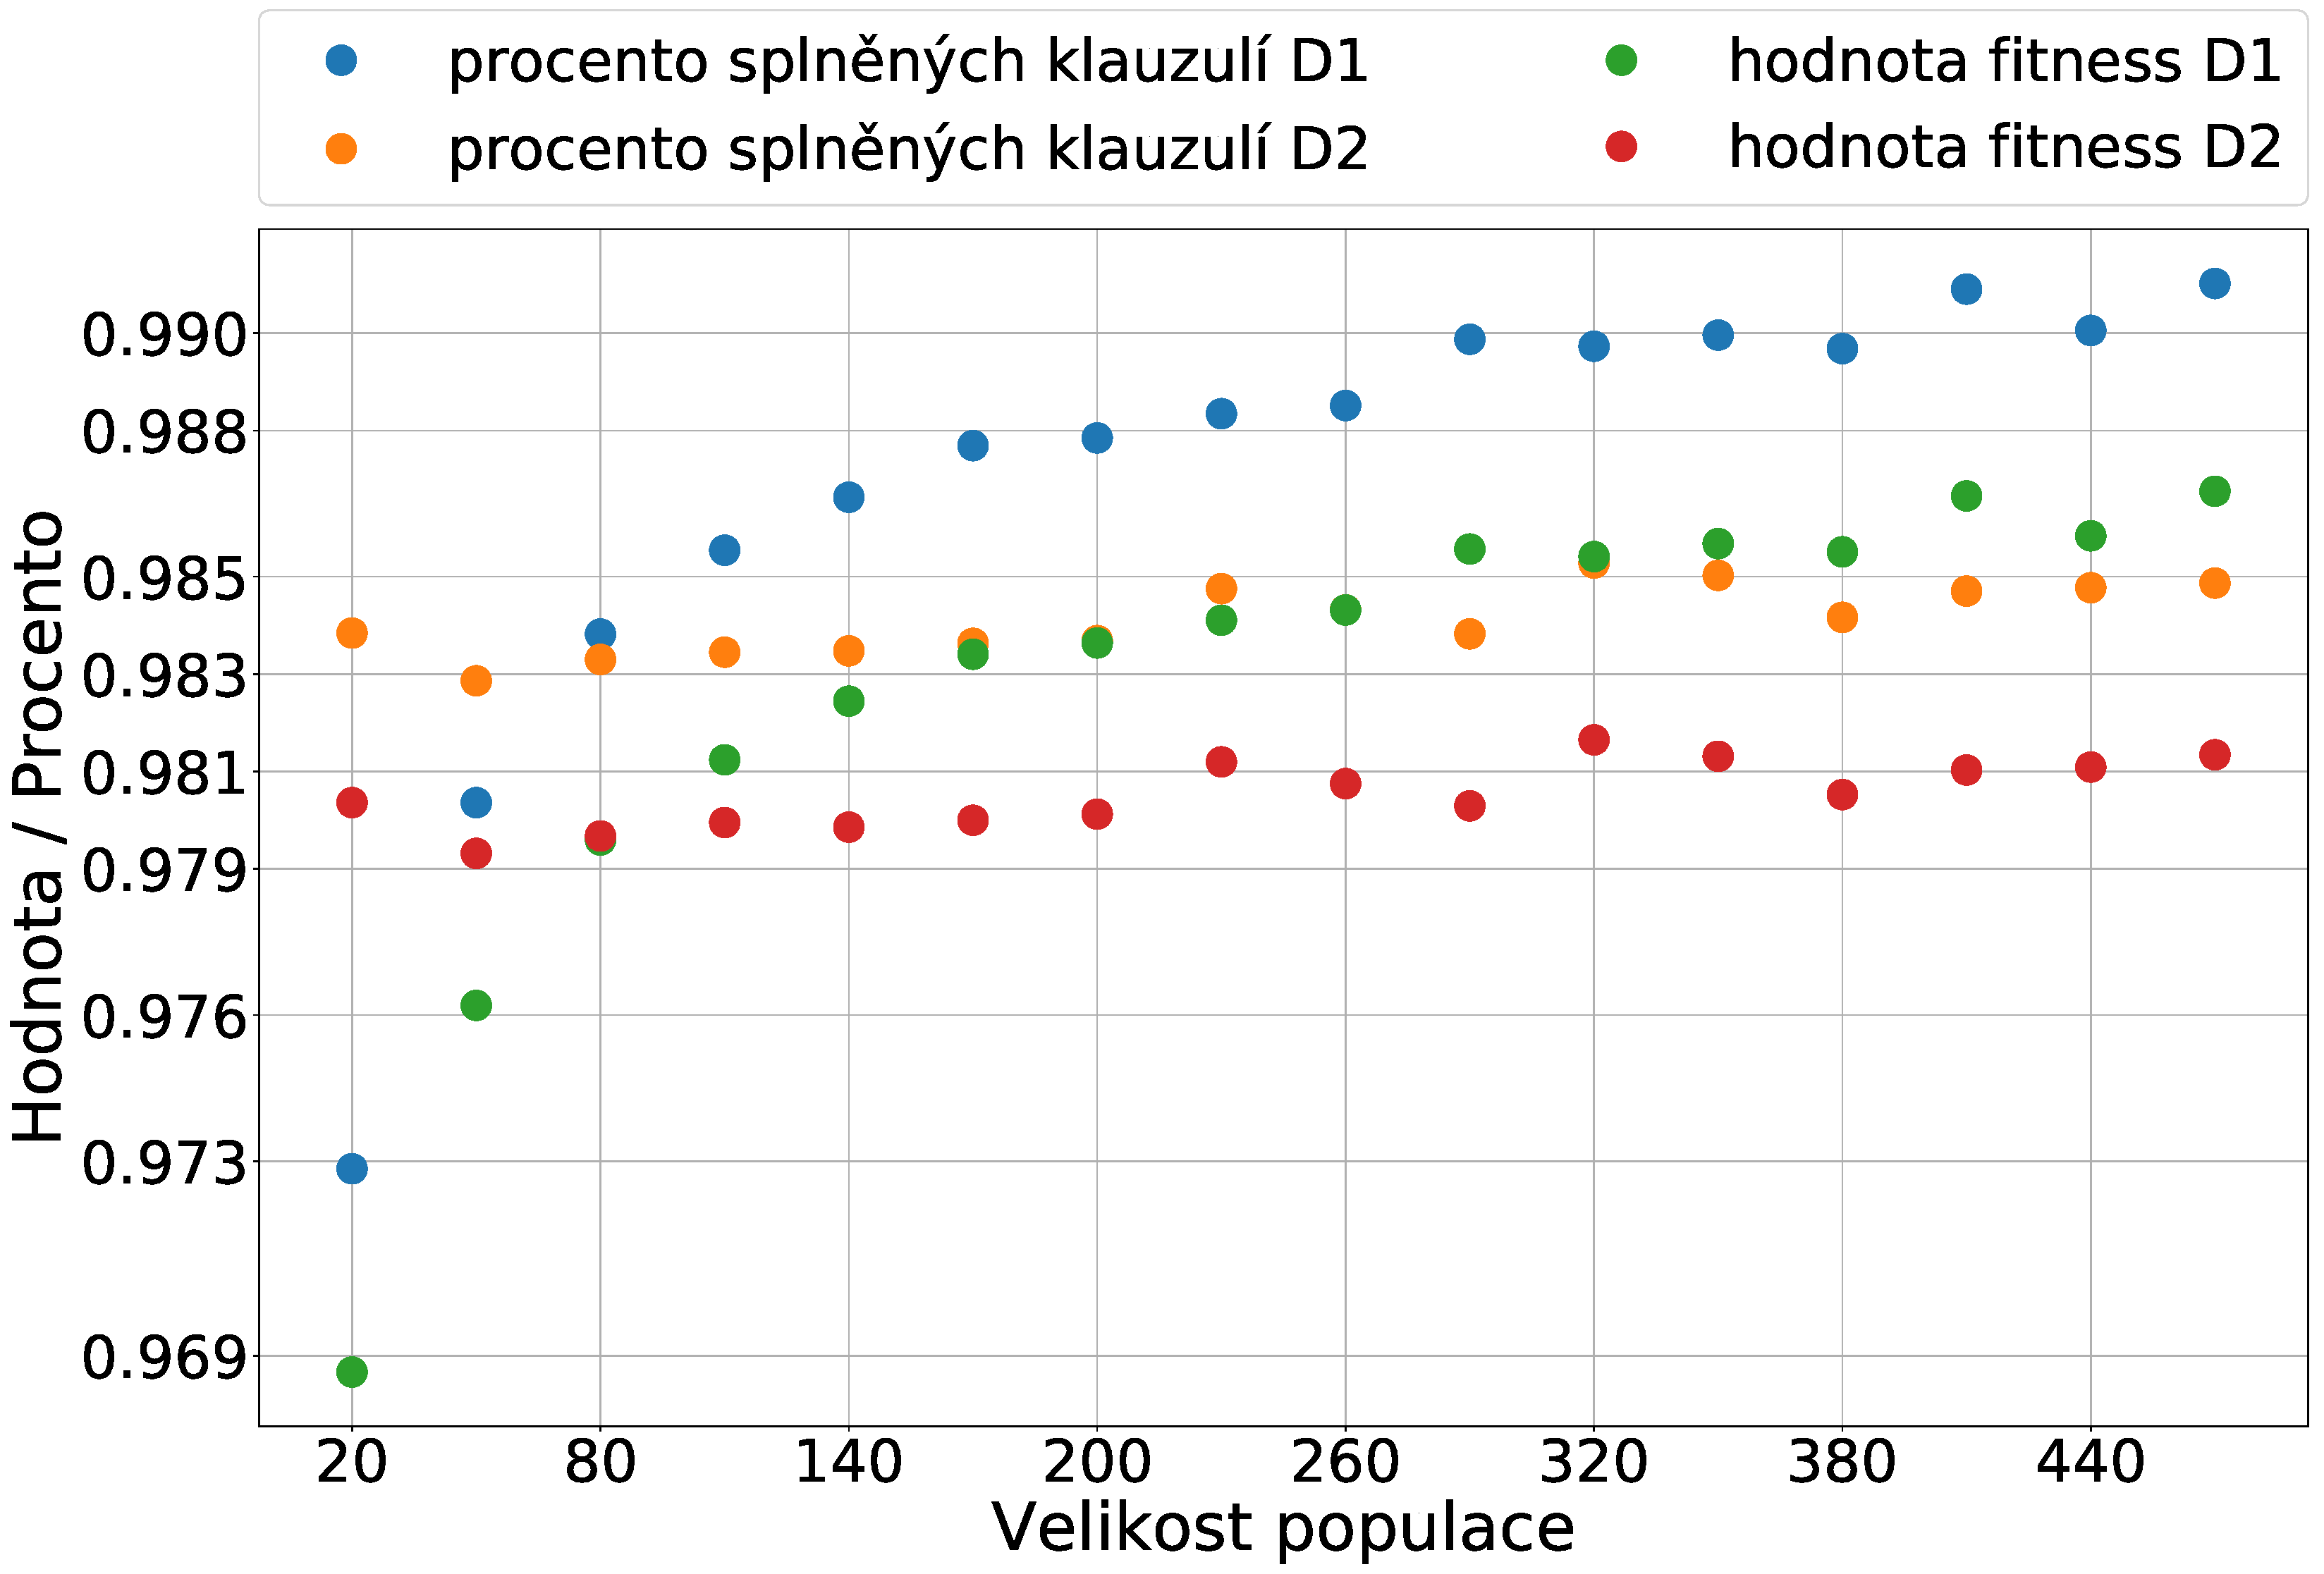
\includegraphics[width=0.55\textwidth]{img/sat_gen_size.pdf} 
\caption{Na obrázku je graf, kde je zobrazena úspěšnost v závislosti na velikosti populace.}
\label{fig:genSize}
\end{center}
\end{wrapfigure}

\subsection{Závislost na velikosti populace}
Na první parametr genetického algoritmu, na který jsem se zaměřil je velikost populace. Ta určuje kolik řešení je vylepšováno a šlechtěno. Optimum tohoto parametru se velice odvíjí od složitosti problému. Já jsem jako základní hodnotu zvolil 100, neboť by mohla být dostačující pro obtížné problémy.

Z experimetu na obrázku \ref{fig:genSize} je vidět, že mnou odhadnutá počáteční velikost se zdá dobrá pro náhodně generované problémy D2, avšak problémy ze SATLIB, které mají všechny poměr klauzulí a proměných okolo 4,3, již tento počet optimální není. A je vidět, že s rostoucím počtem roste i úspěšnost na problémech D1. Z těchto měření bych tedy jako základní parametr algoritmu pro řešení problémů nastavil hodnotu 400. Problém vážené splnitelnosti formule v normální tvaru patří mezi velice obtížné problémy.


\begin{figure}
	\centering
	\begin{minipage}[c]{0.74\textwidth}
        \centering 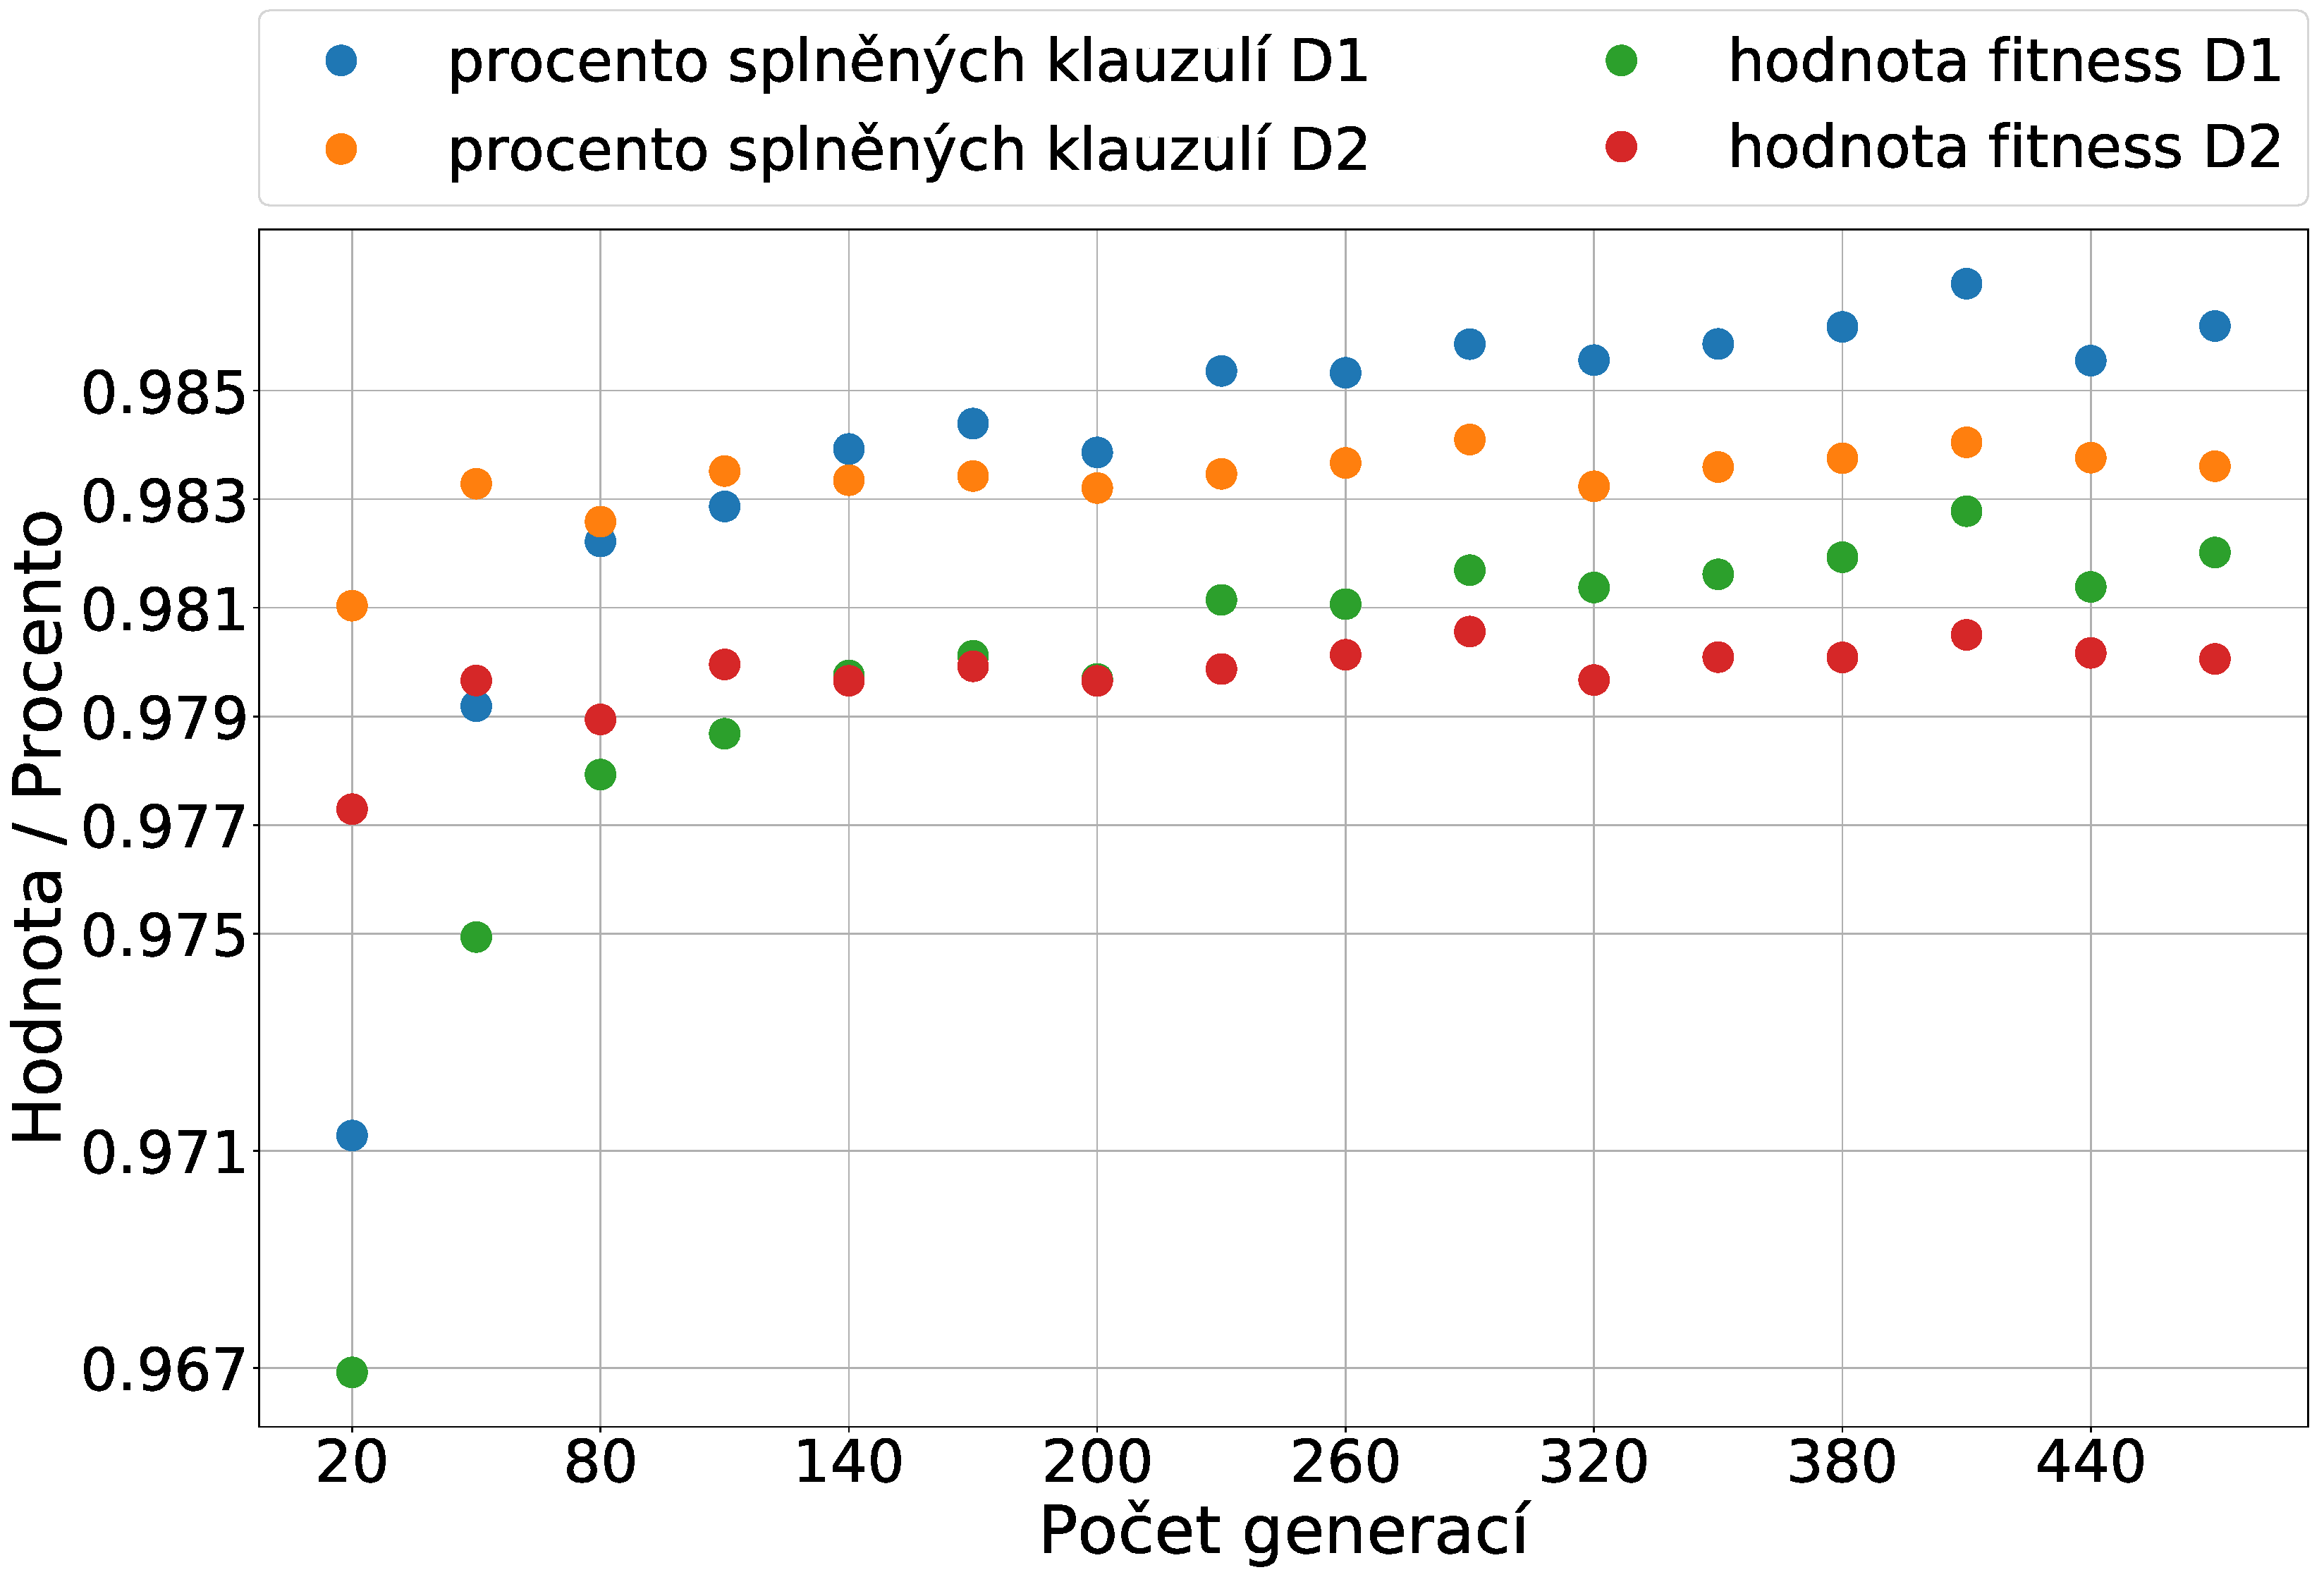
\includegraphics[width=\textwidth]{img/sat_gen_count.pdf} 
    \end{minipage}
    \\
    \begin{minipage}[c]{0.325\textwidth}
        \centering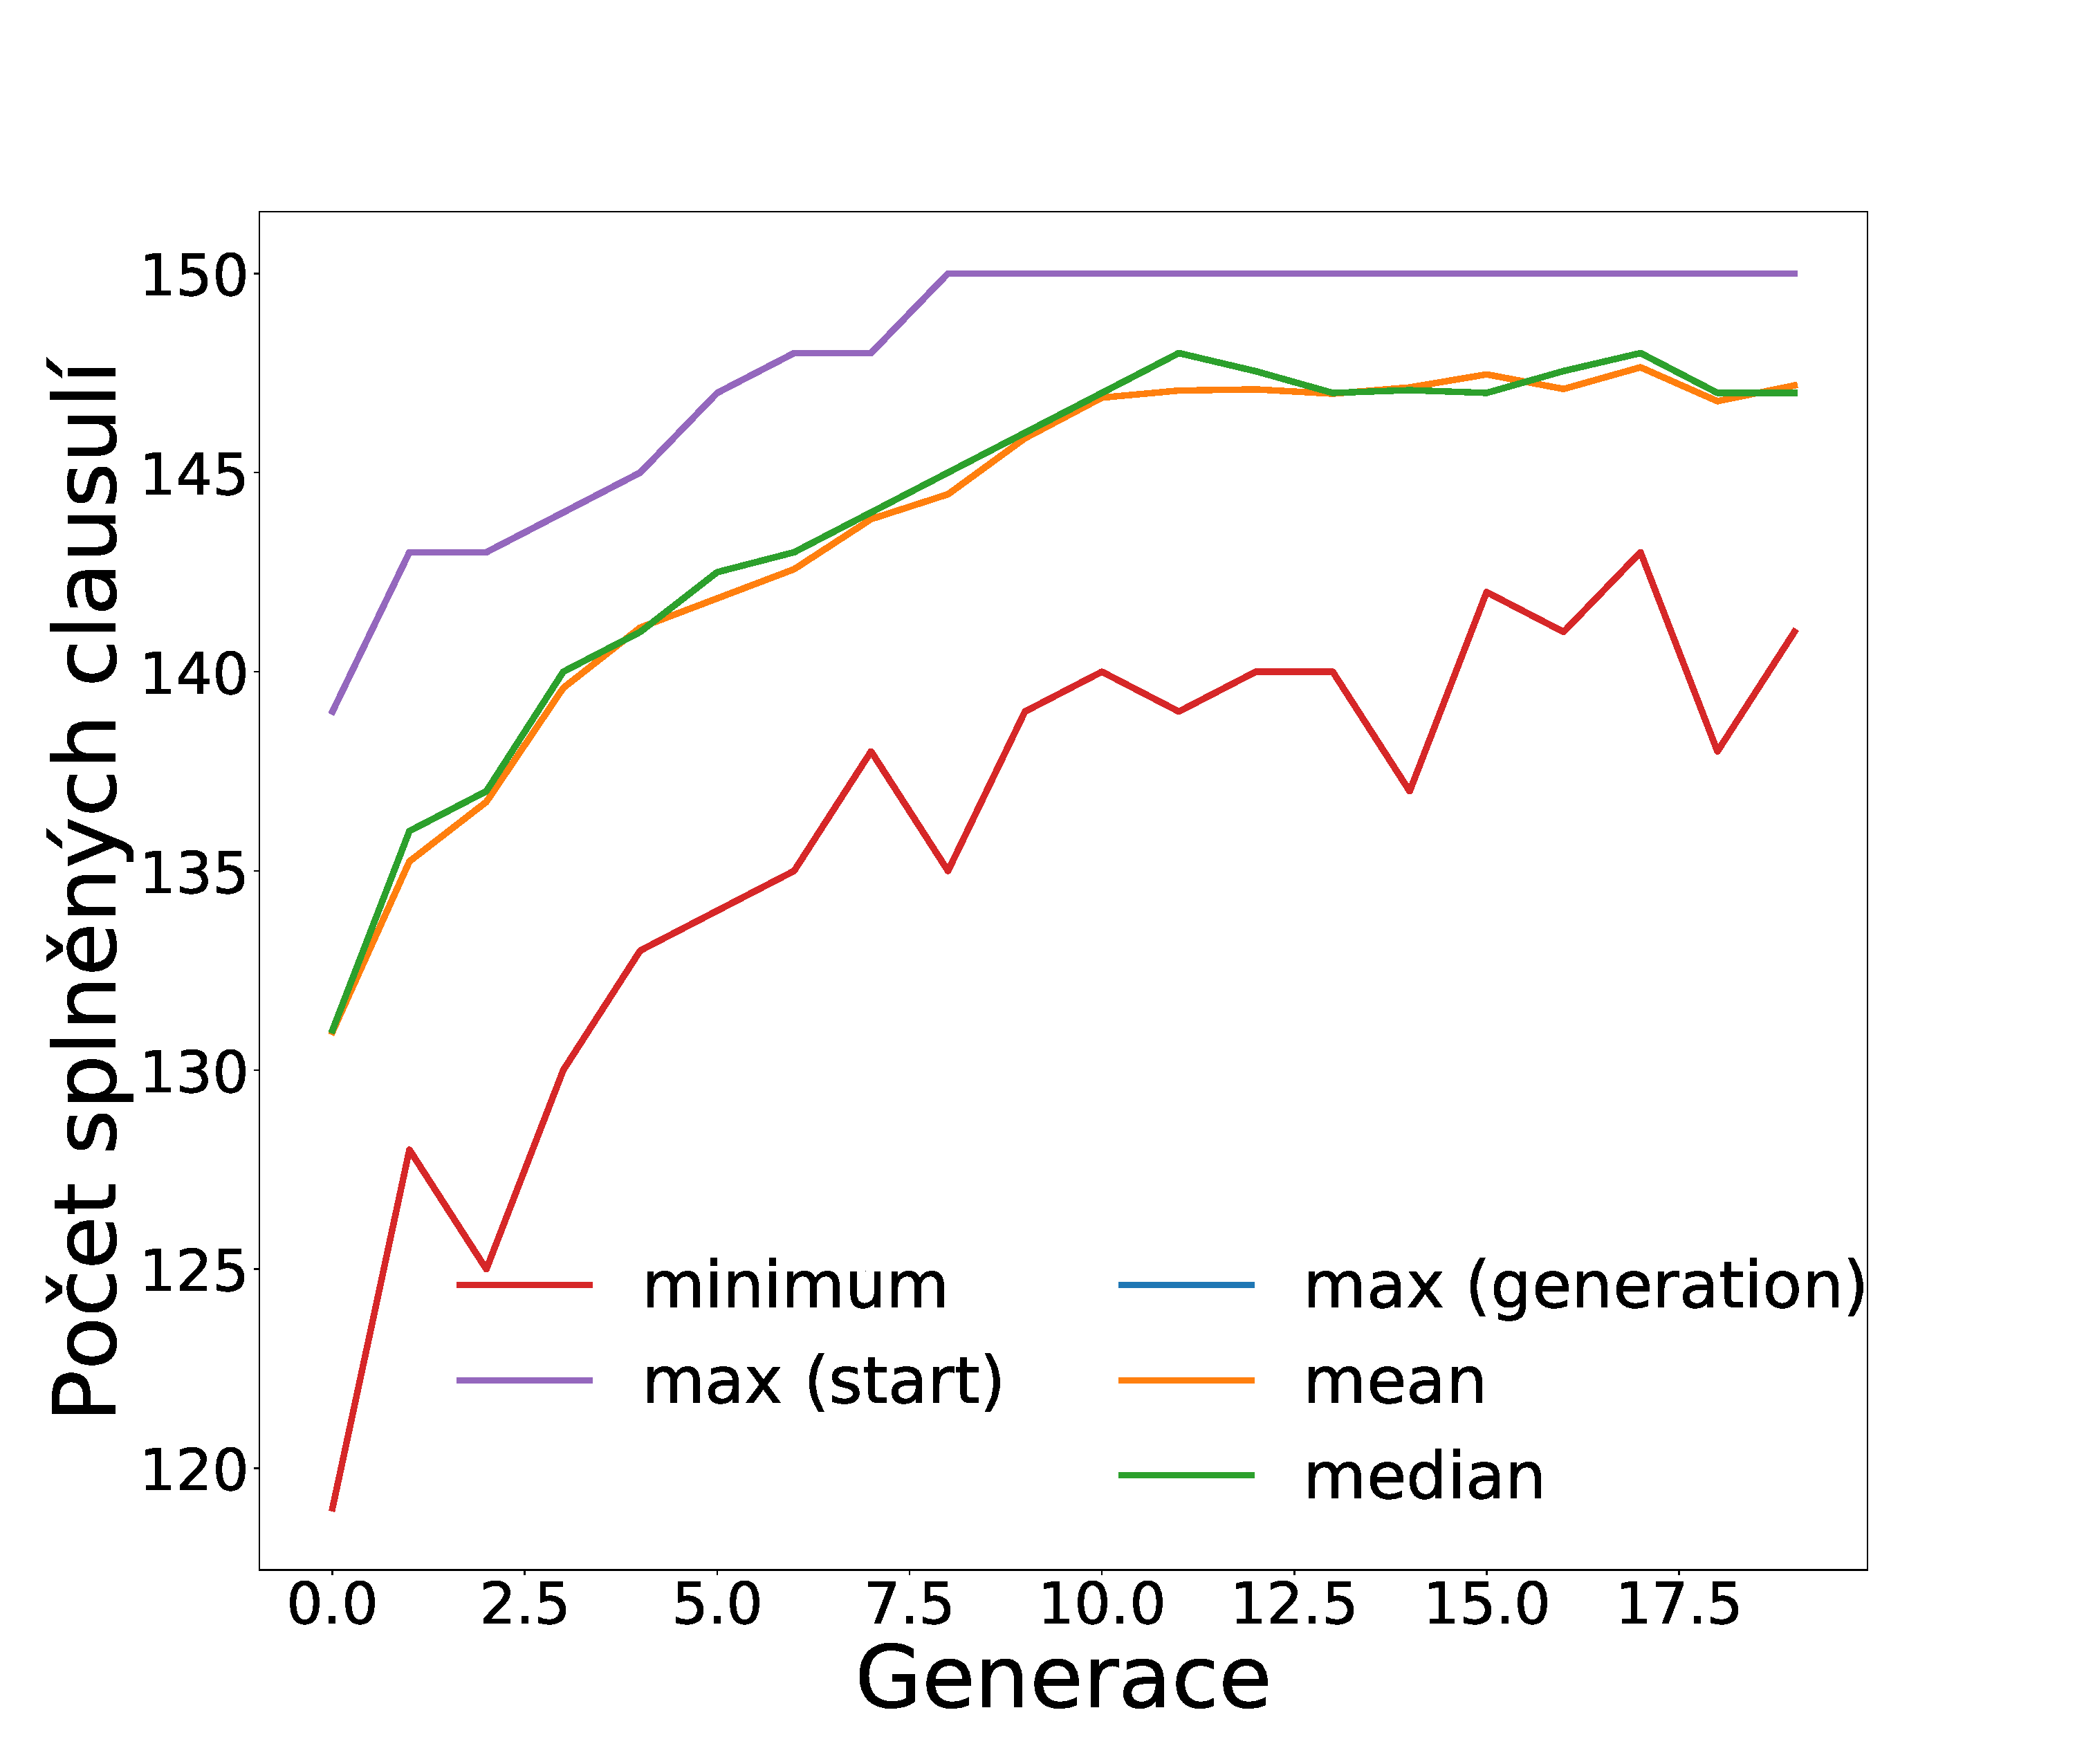
\includegraphics[width=\textwidth]{img/gc1p.pdf} 
    \end{minipage}
    \begin{minipage}[c]{0.325\textwidth}
        \centering 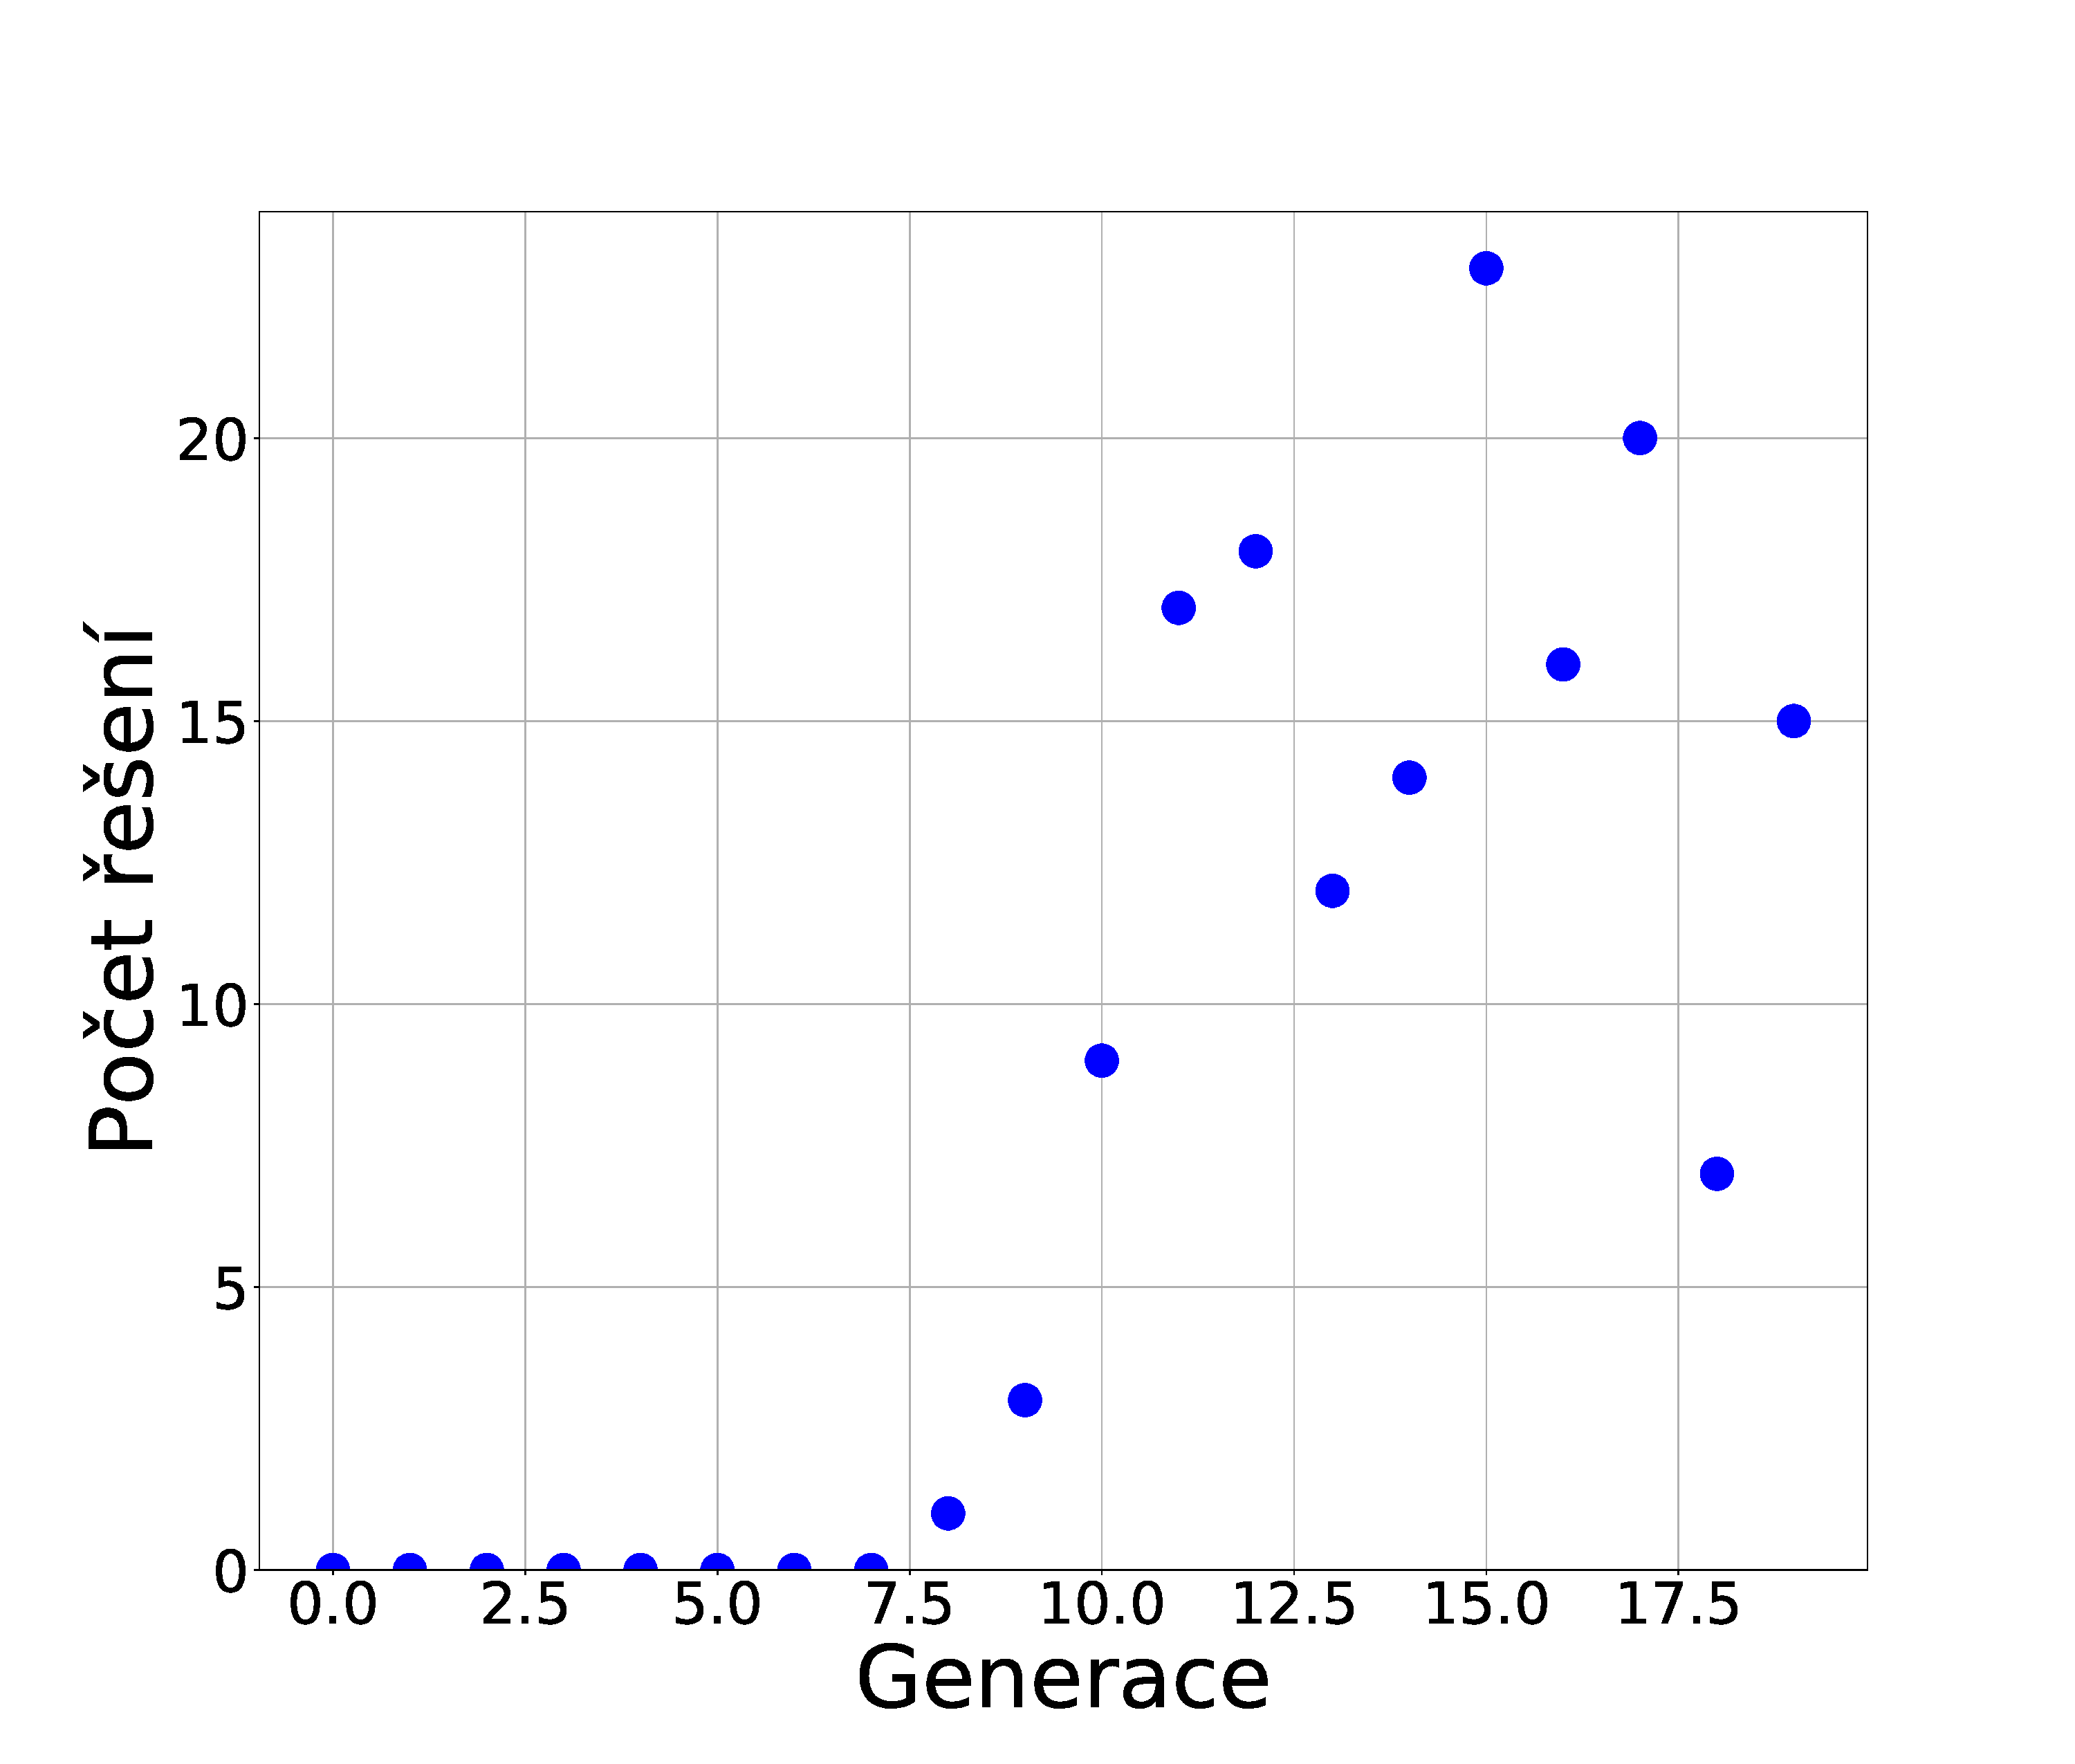
\includegraphics[width=\textwidth]{img/gc1s.pdf} 
    \end{minipage}
    \begin{minipage}[c]{0.325\textwidth}
        \centering 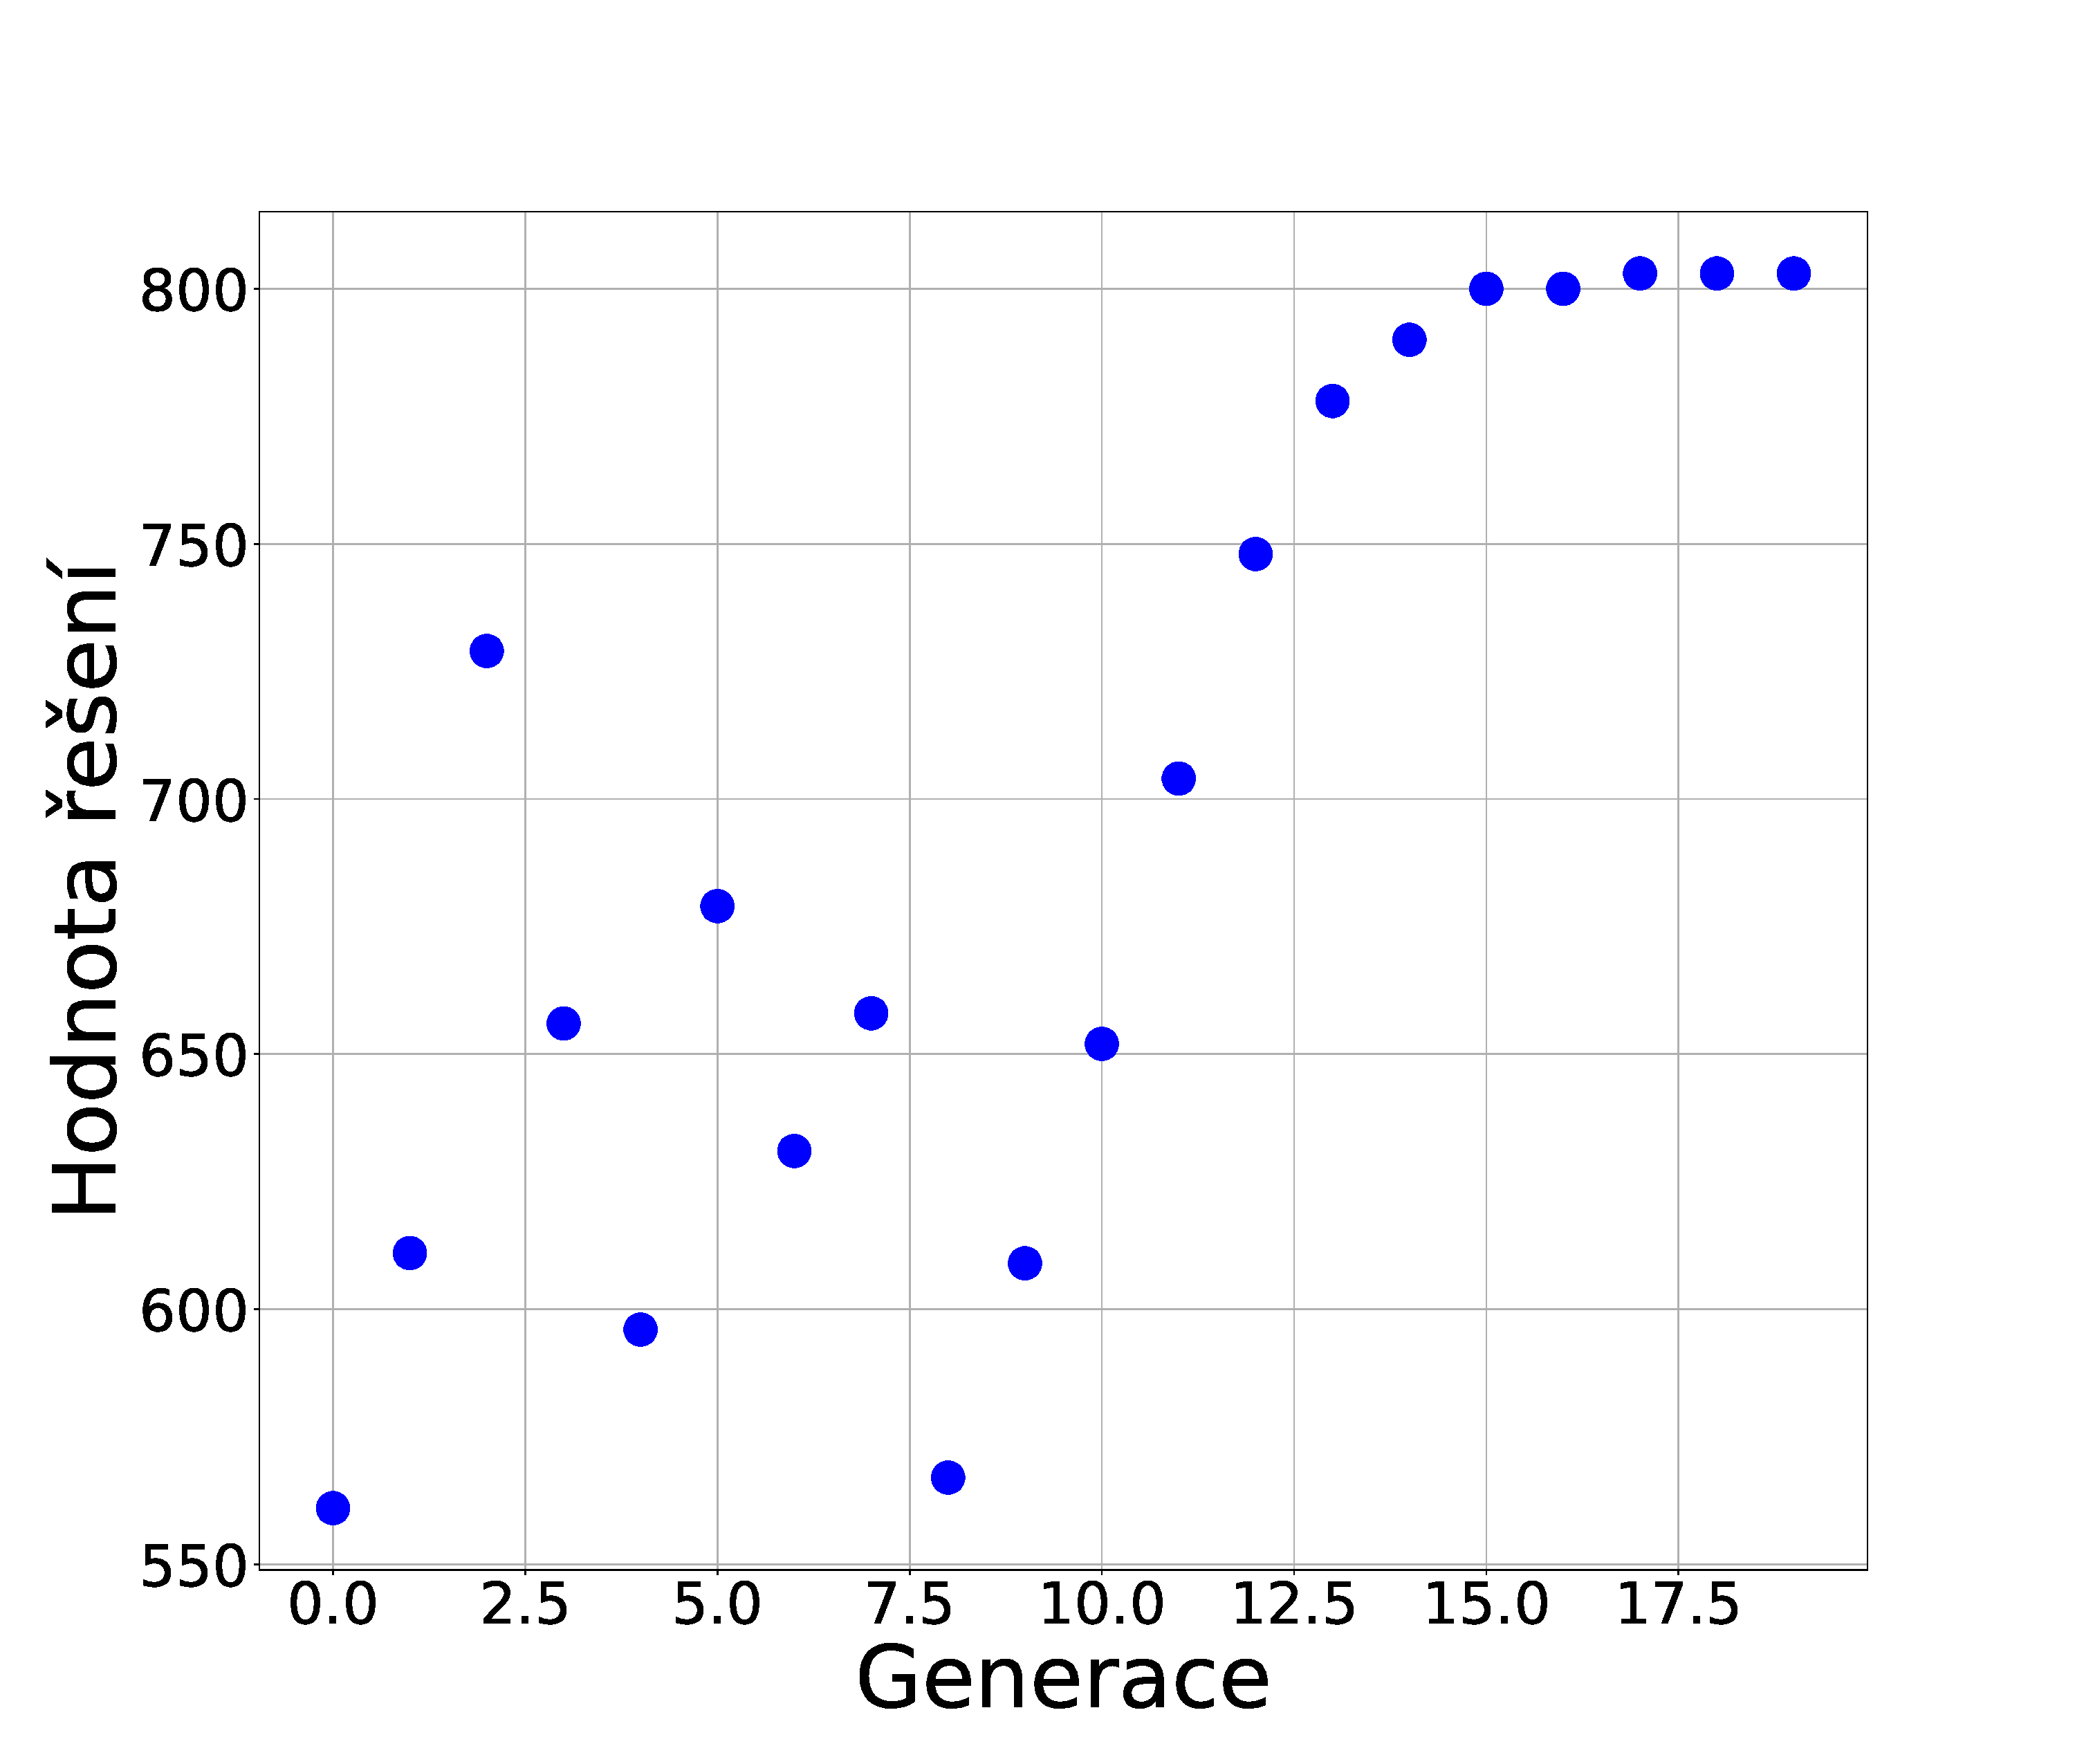
\includegraphics[width=\textwidth]{img/gc1w.pdf} 
    \end{minipage}
    \\
    \begin{minipage}[c]{0.325\textwidth}
        \centering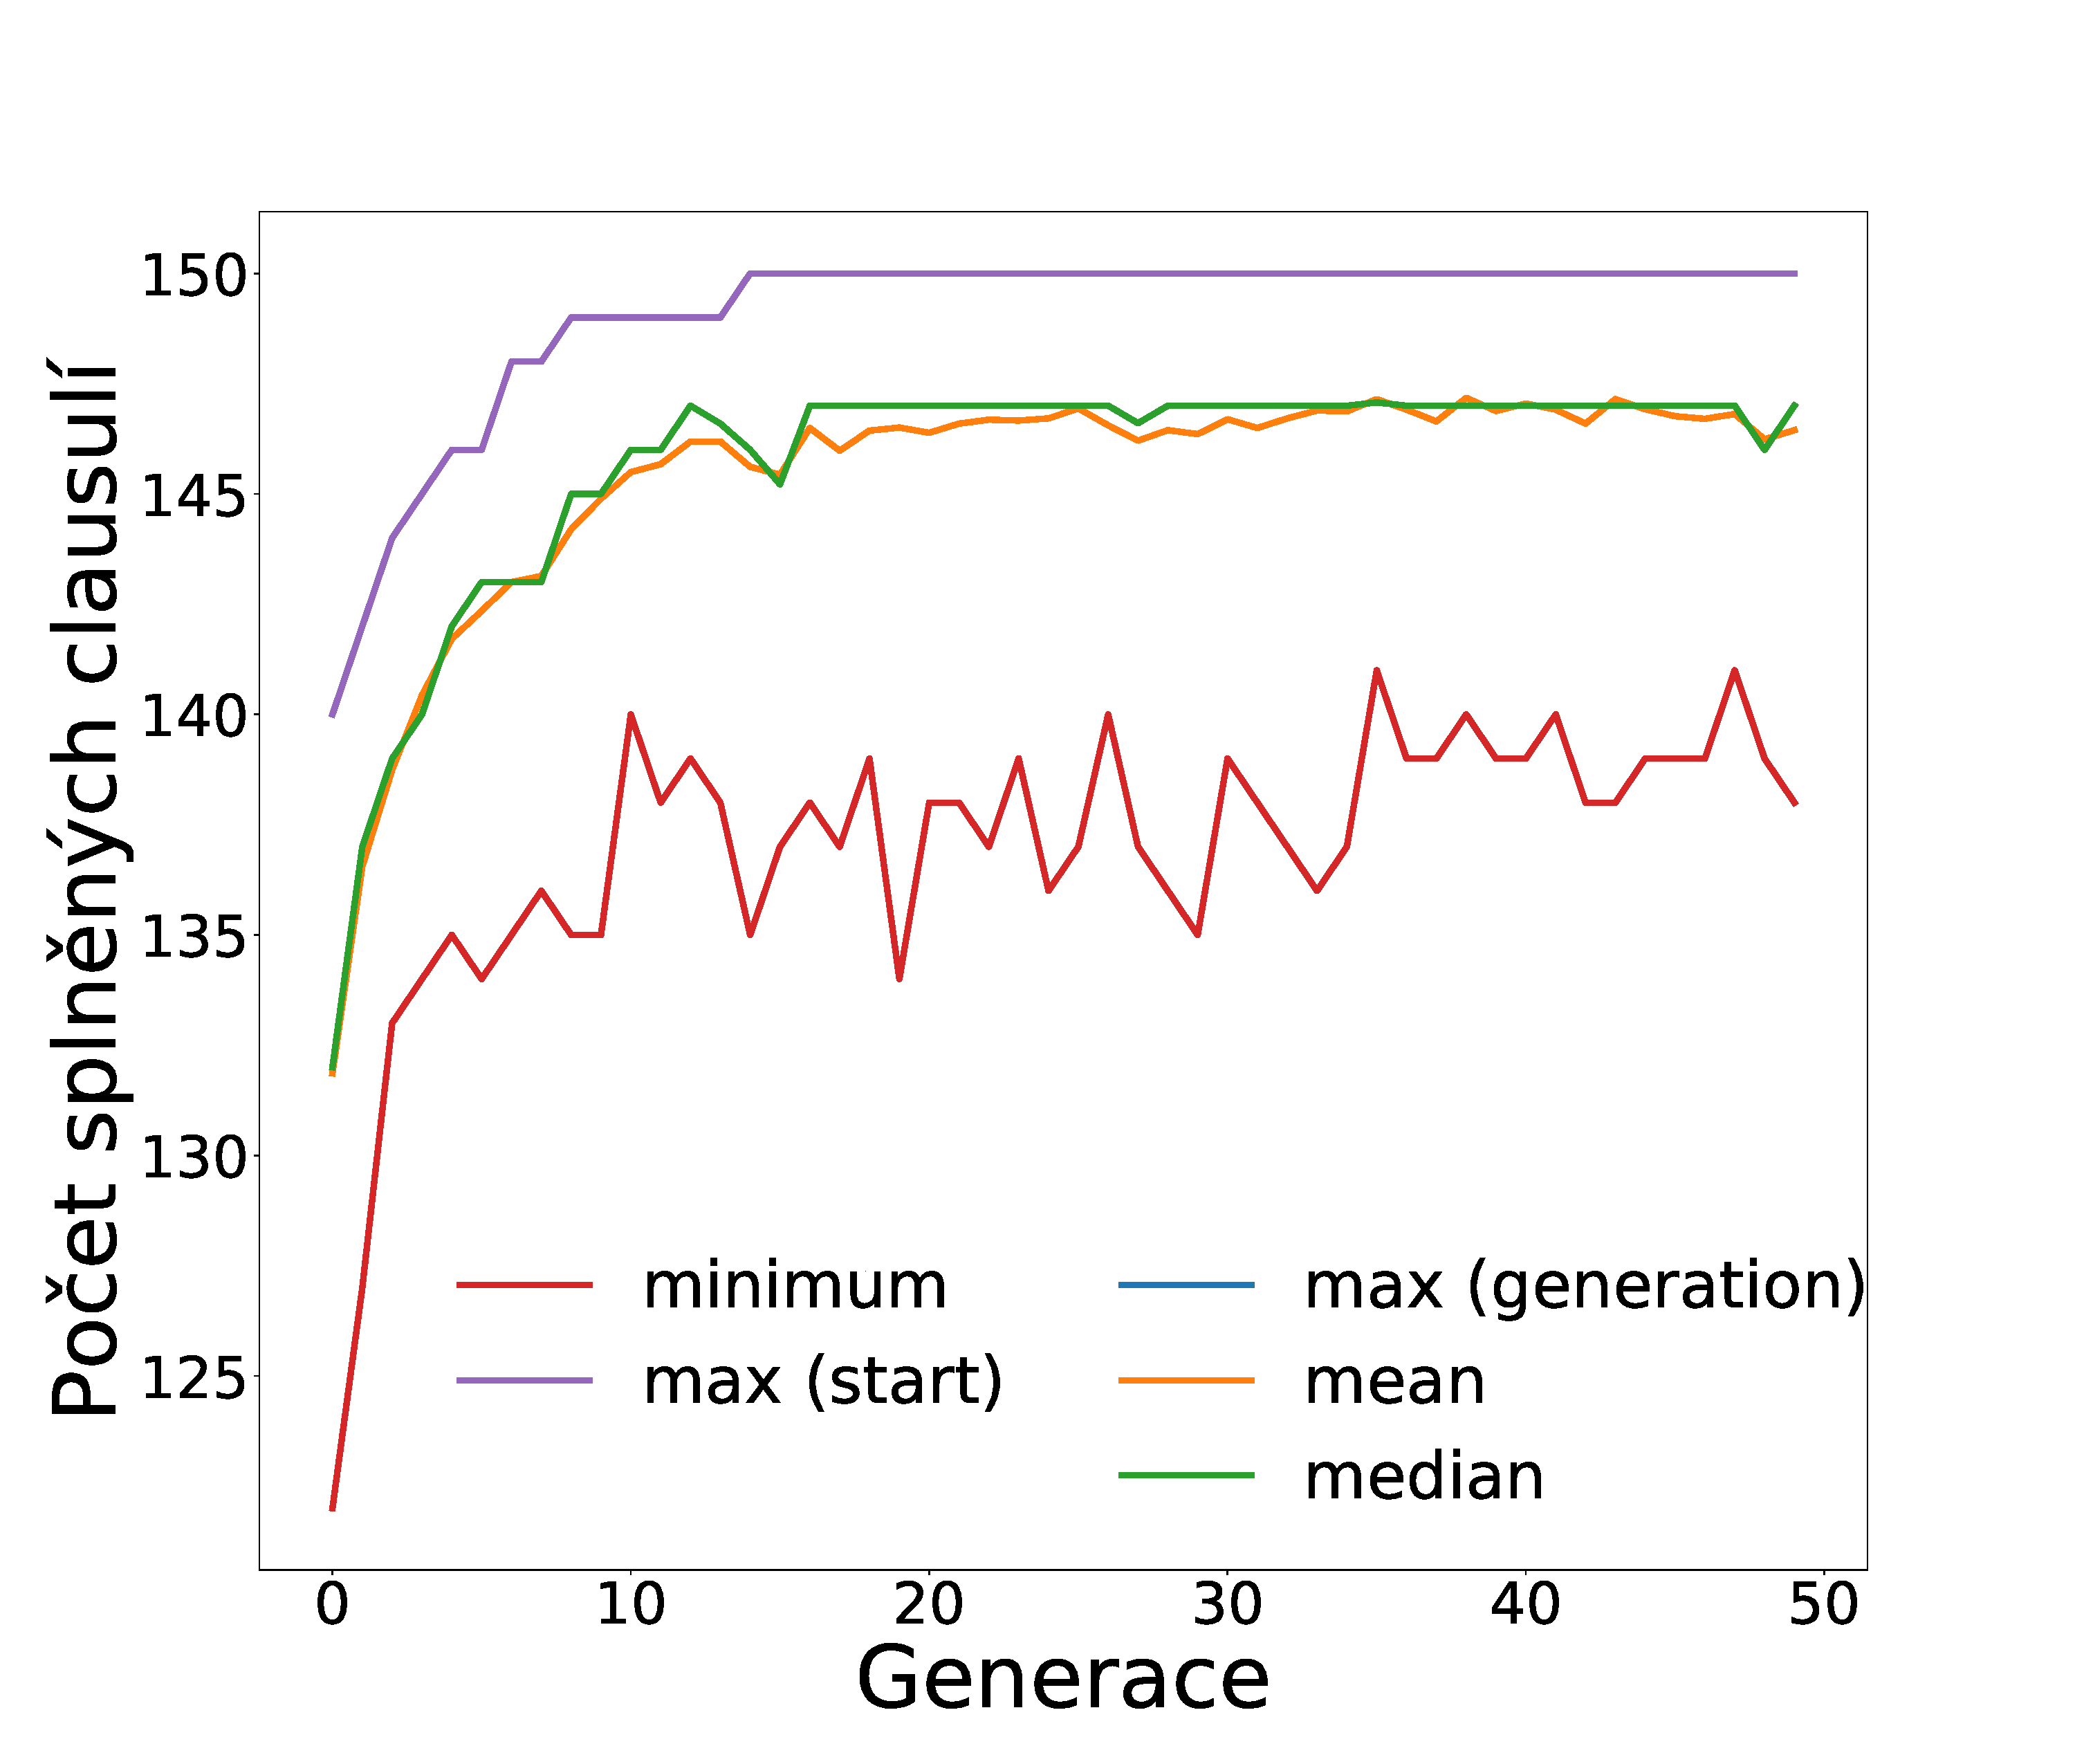
\includegraphics[width=\textwidth]{img/gc2p.pdf} 
    \end{minipage}
    \begin{minipage}[c]{0.325\textwidth}
        \centering 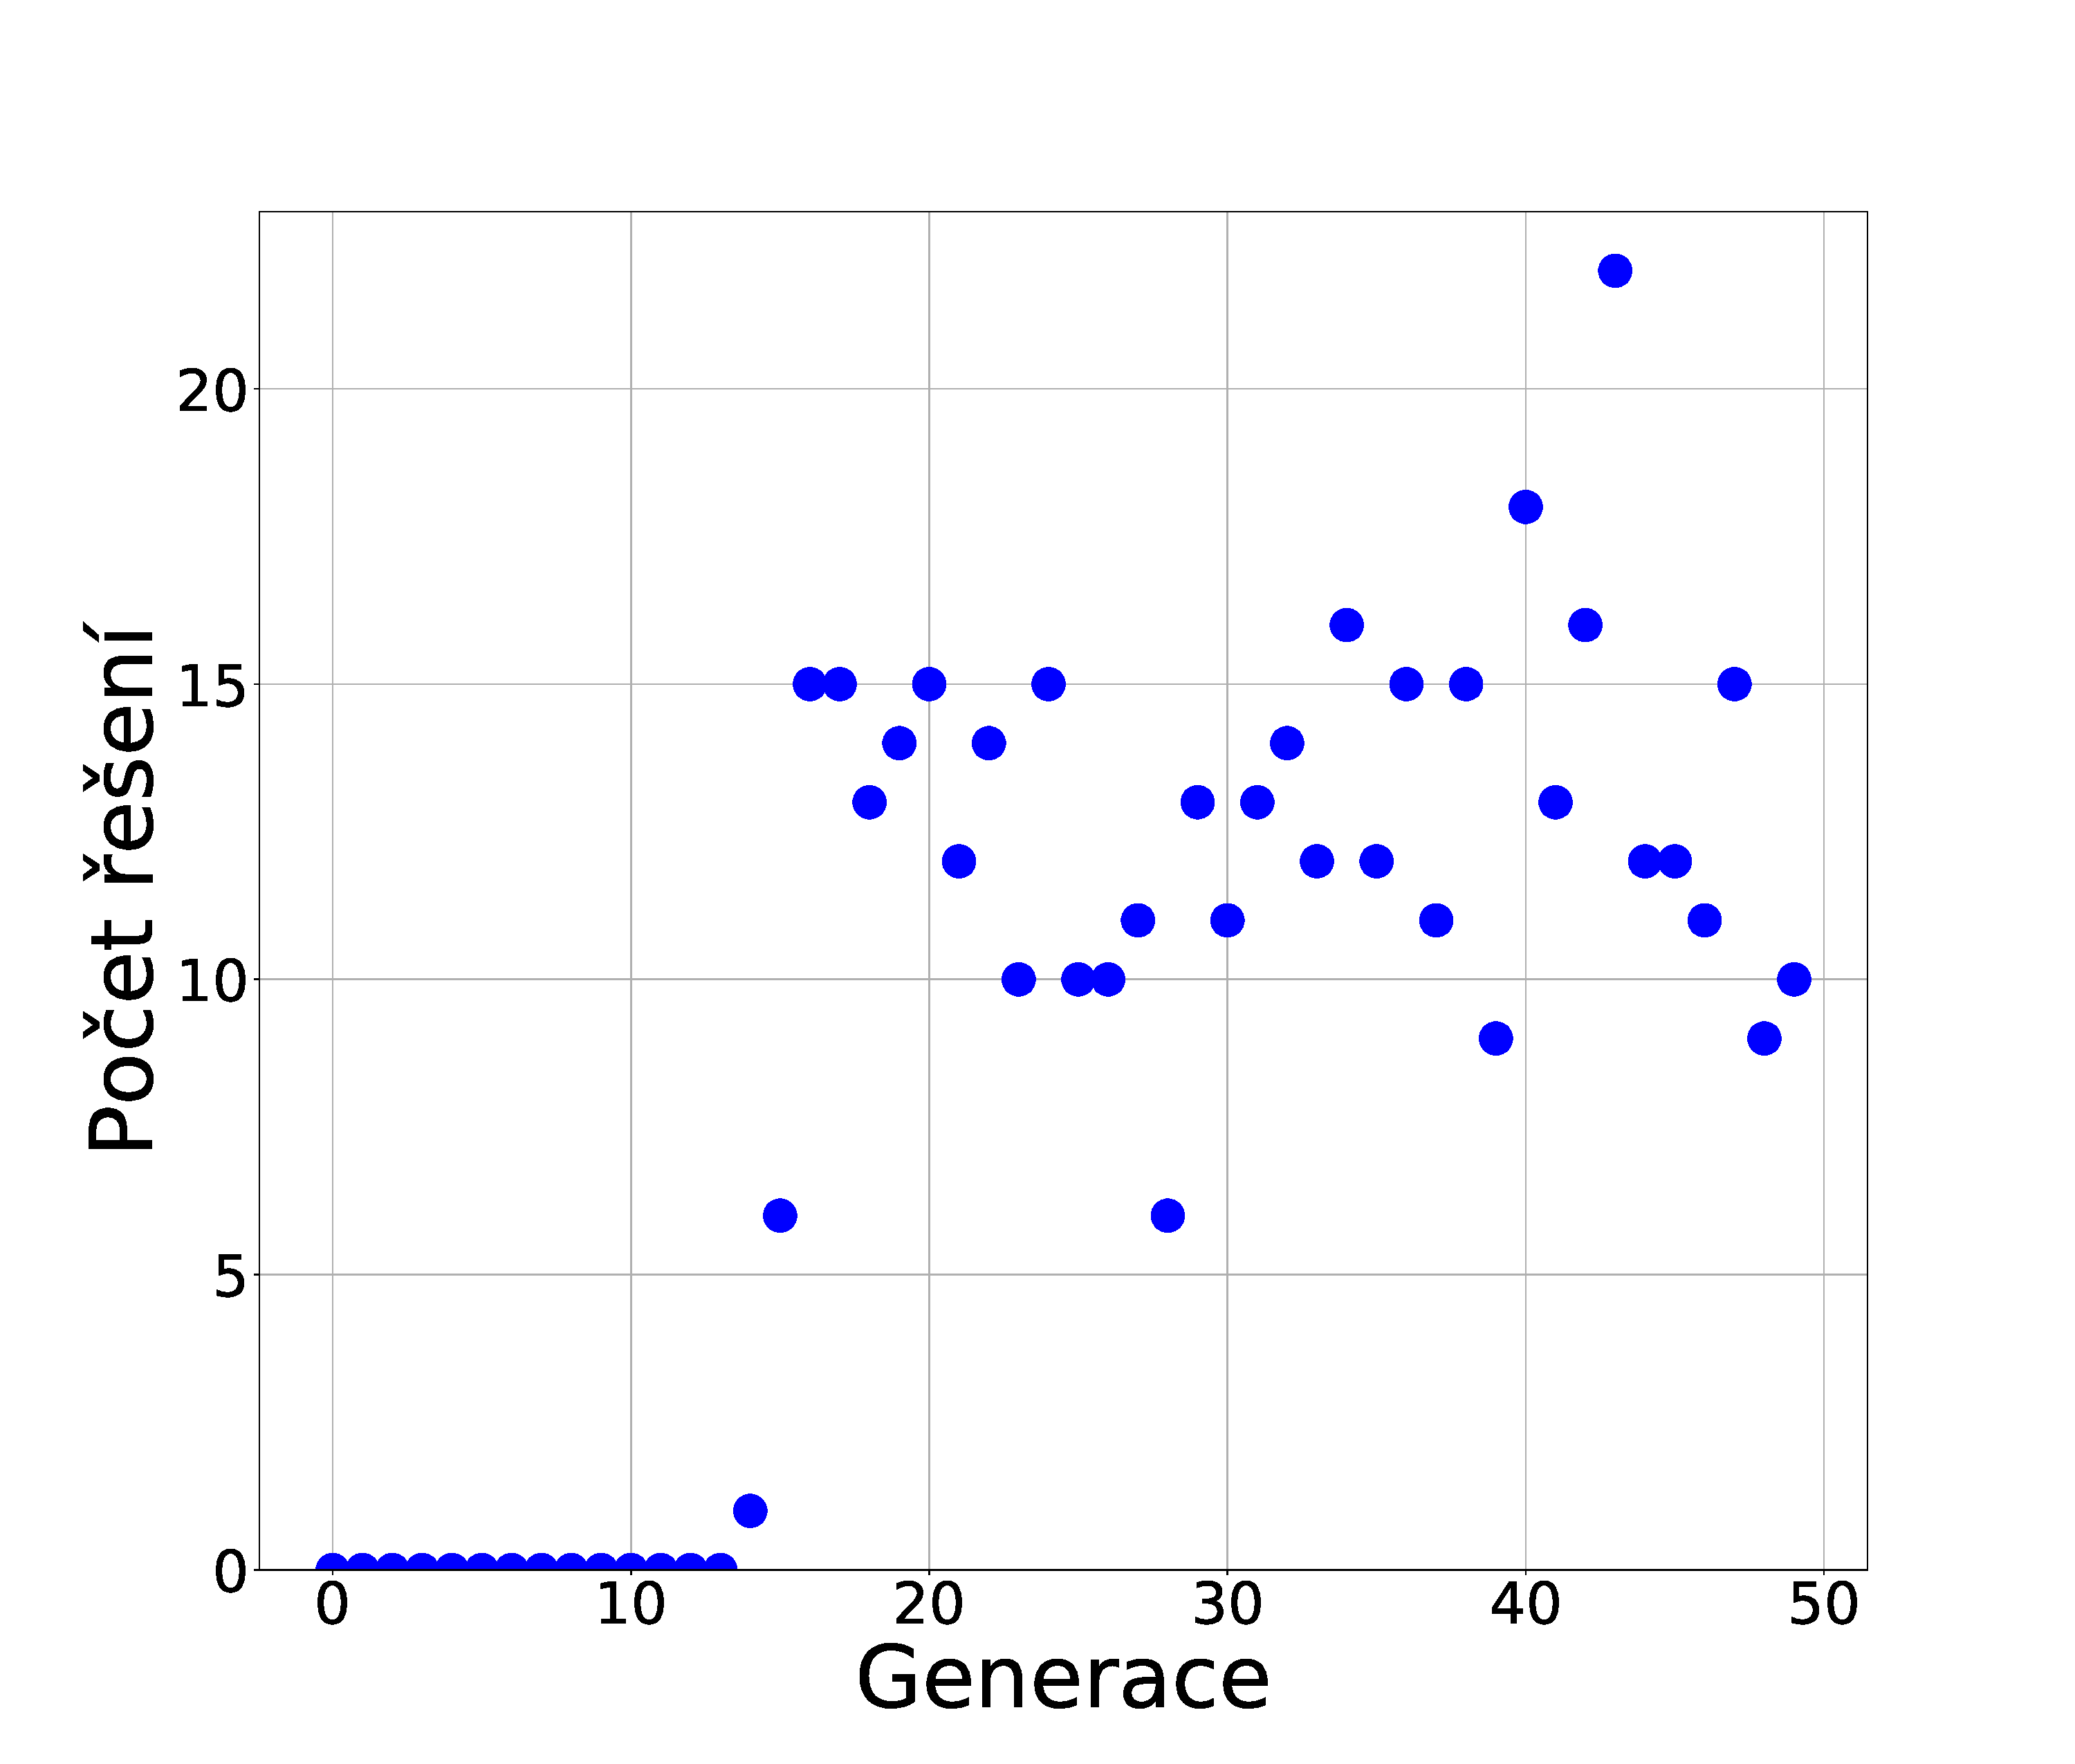
\includegraphics[width=\textwidth]{img/gc2s.pdf} 
    \end{minipage}
    \begin{minipage}[c]{0.325\textwidth}
        \centering 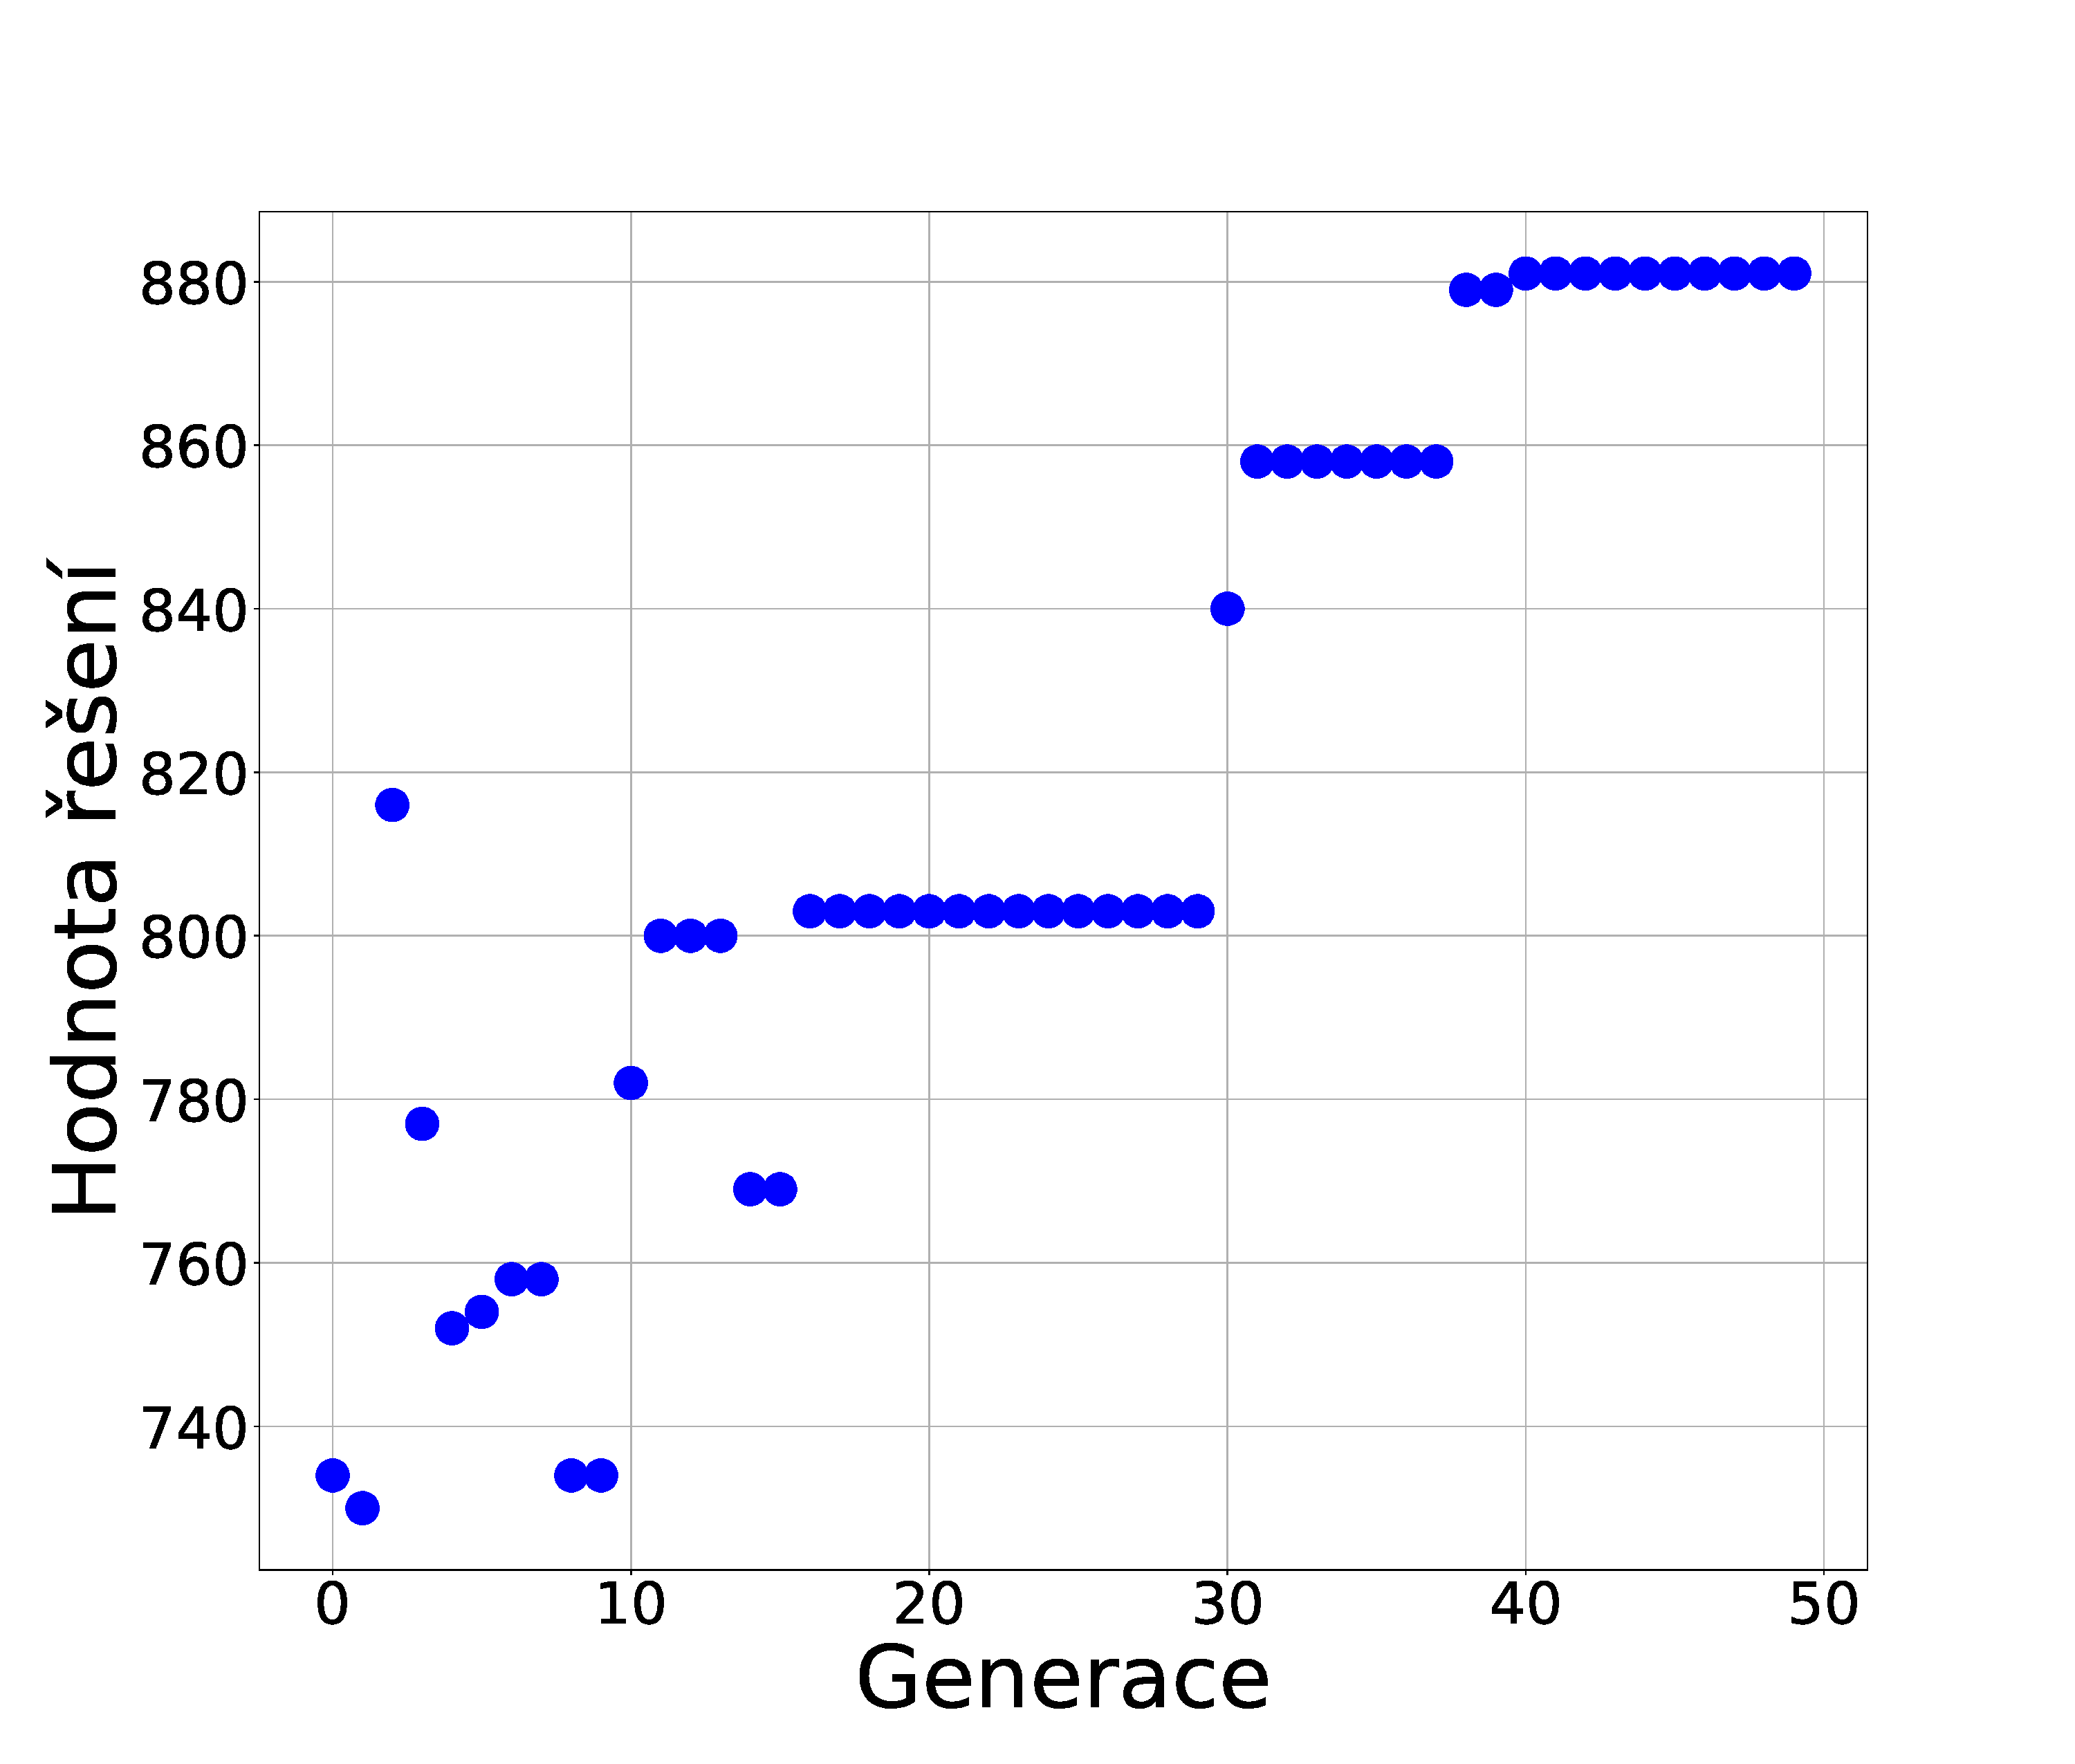
\includegraphics[width=\textwidth]{img/gc2w.pdf} 
    \end{minipage}
    \\
    \begin{minipage}[c]{0.325\textwidth}
        \centering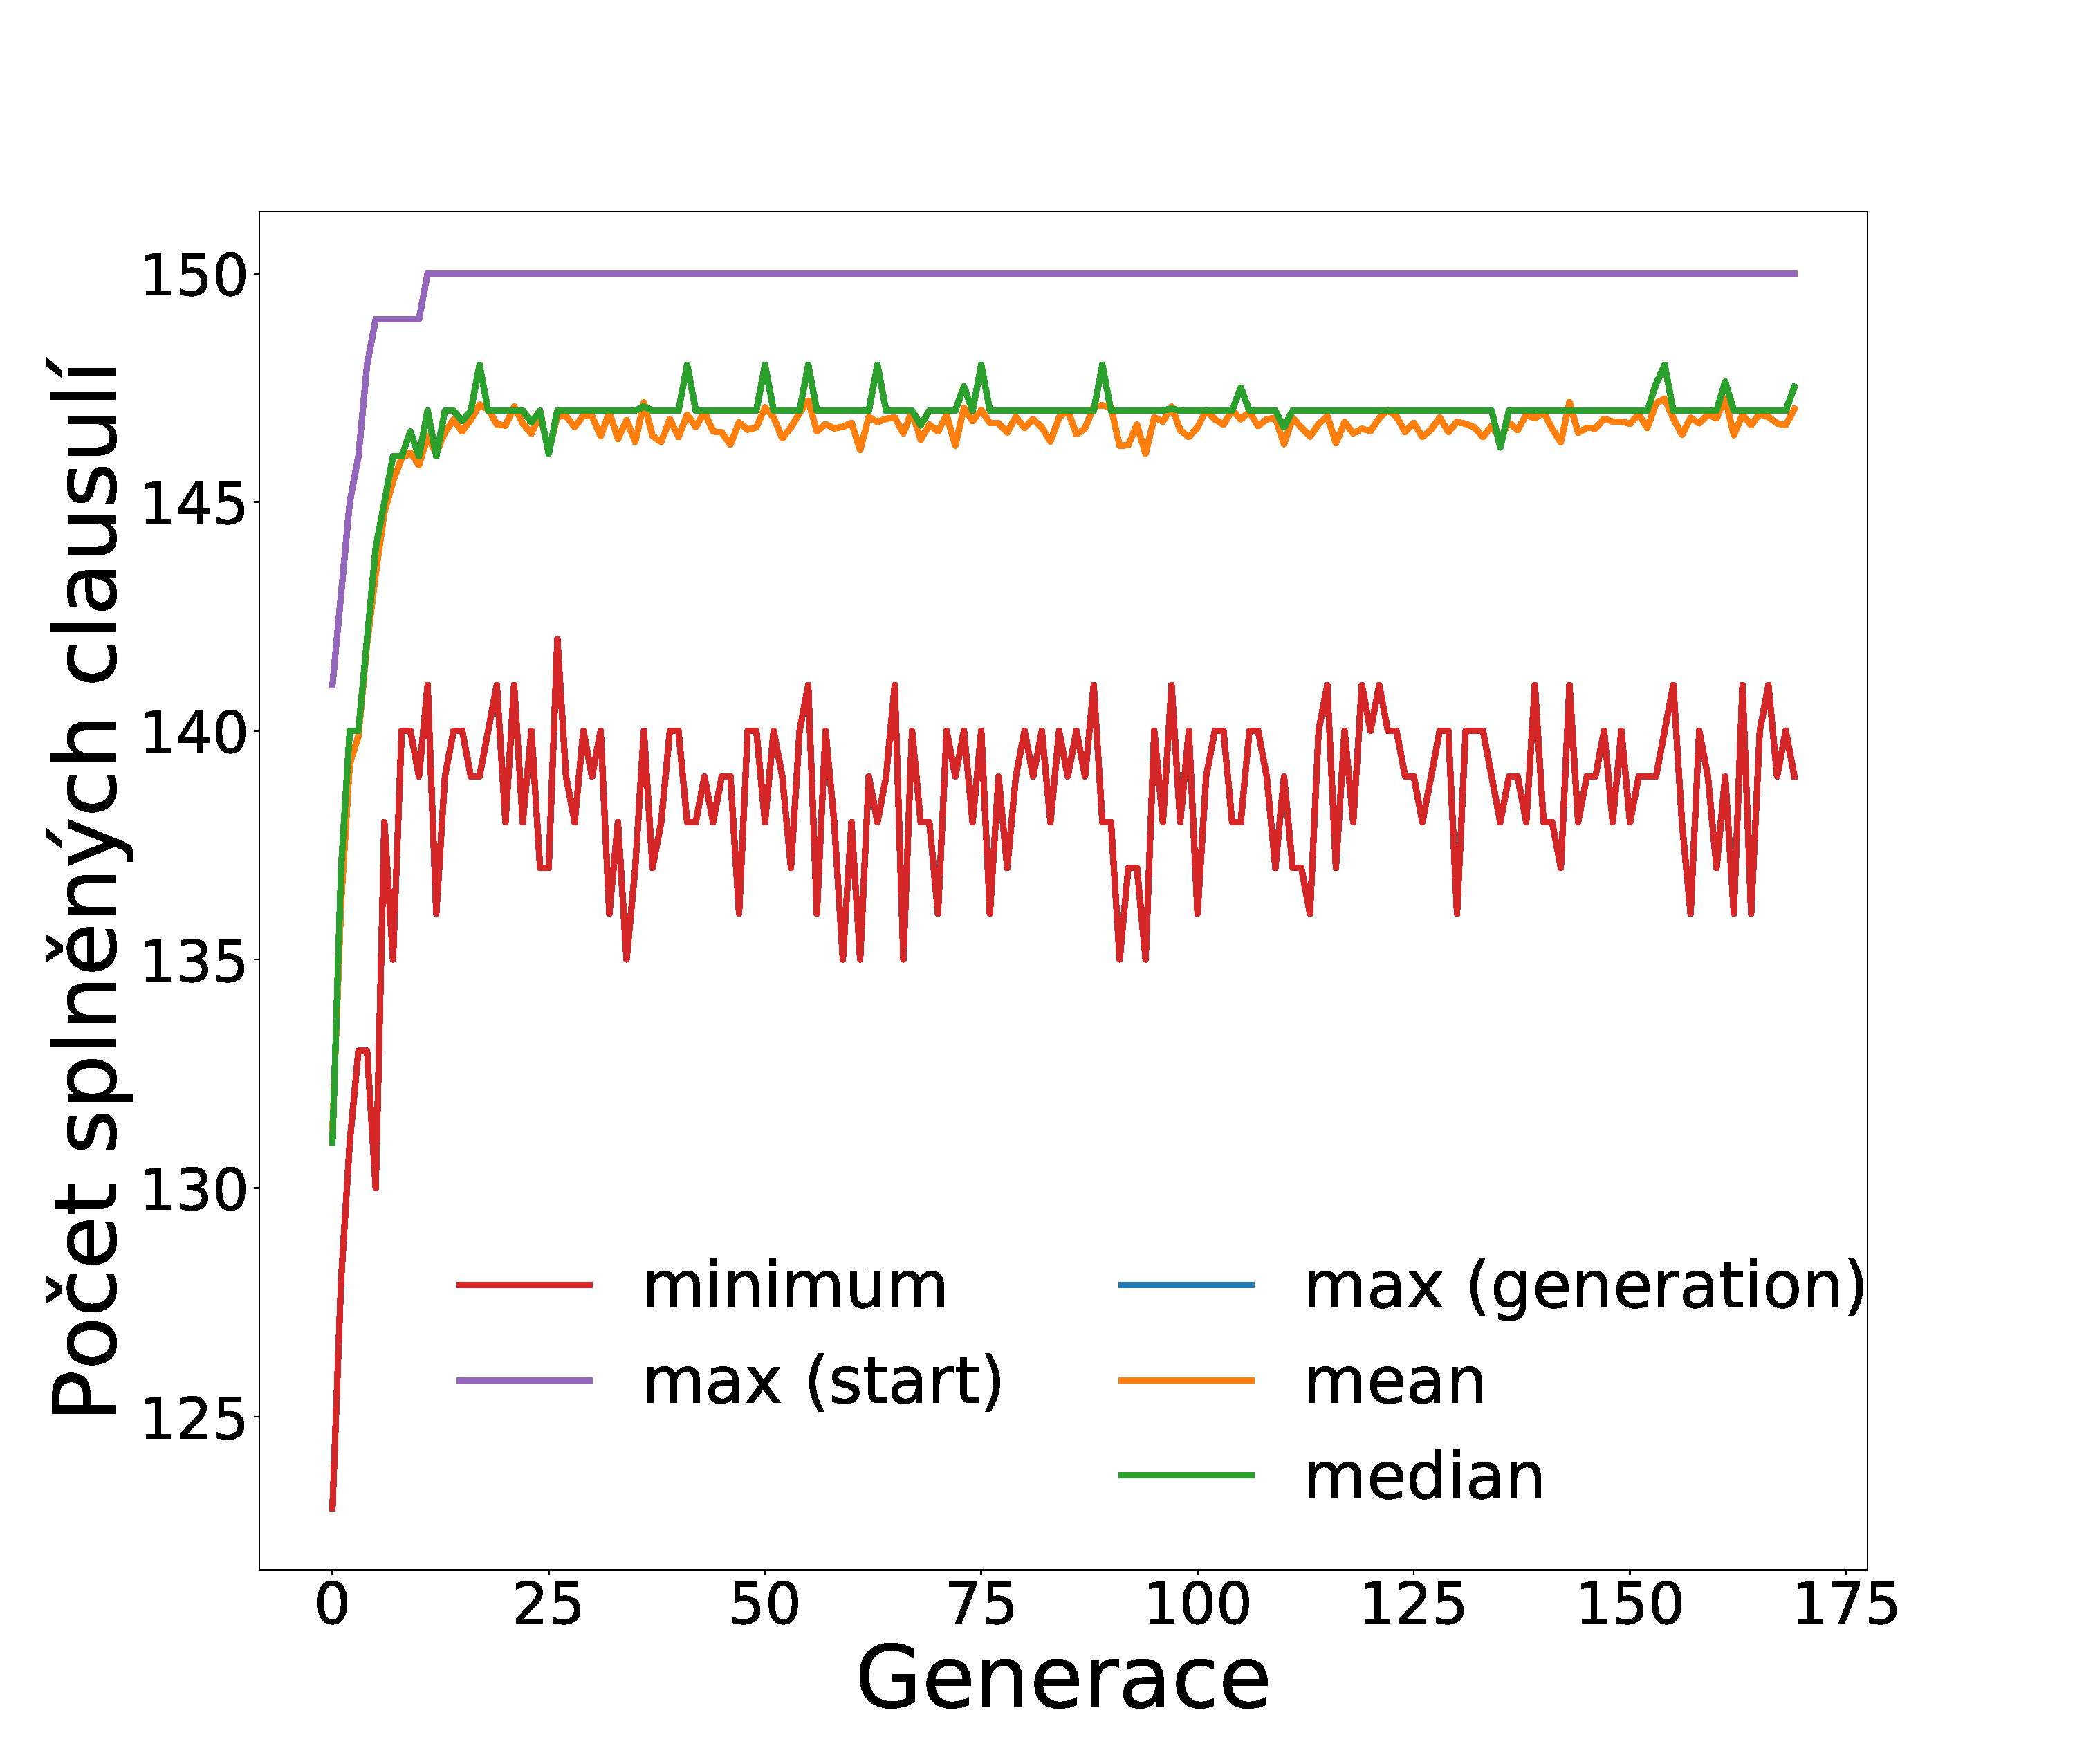
\includegraphics[width=\textwidth]{img/gc3p.pdf} 
    \end{minipage}
    \begin{minipage}[c]{0.325\textwidth}
        \centering 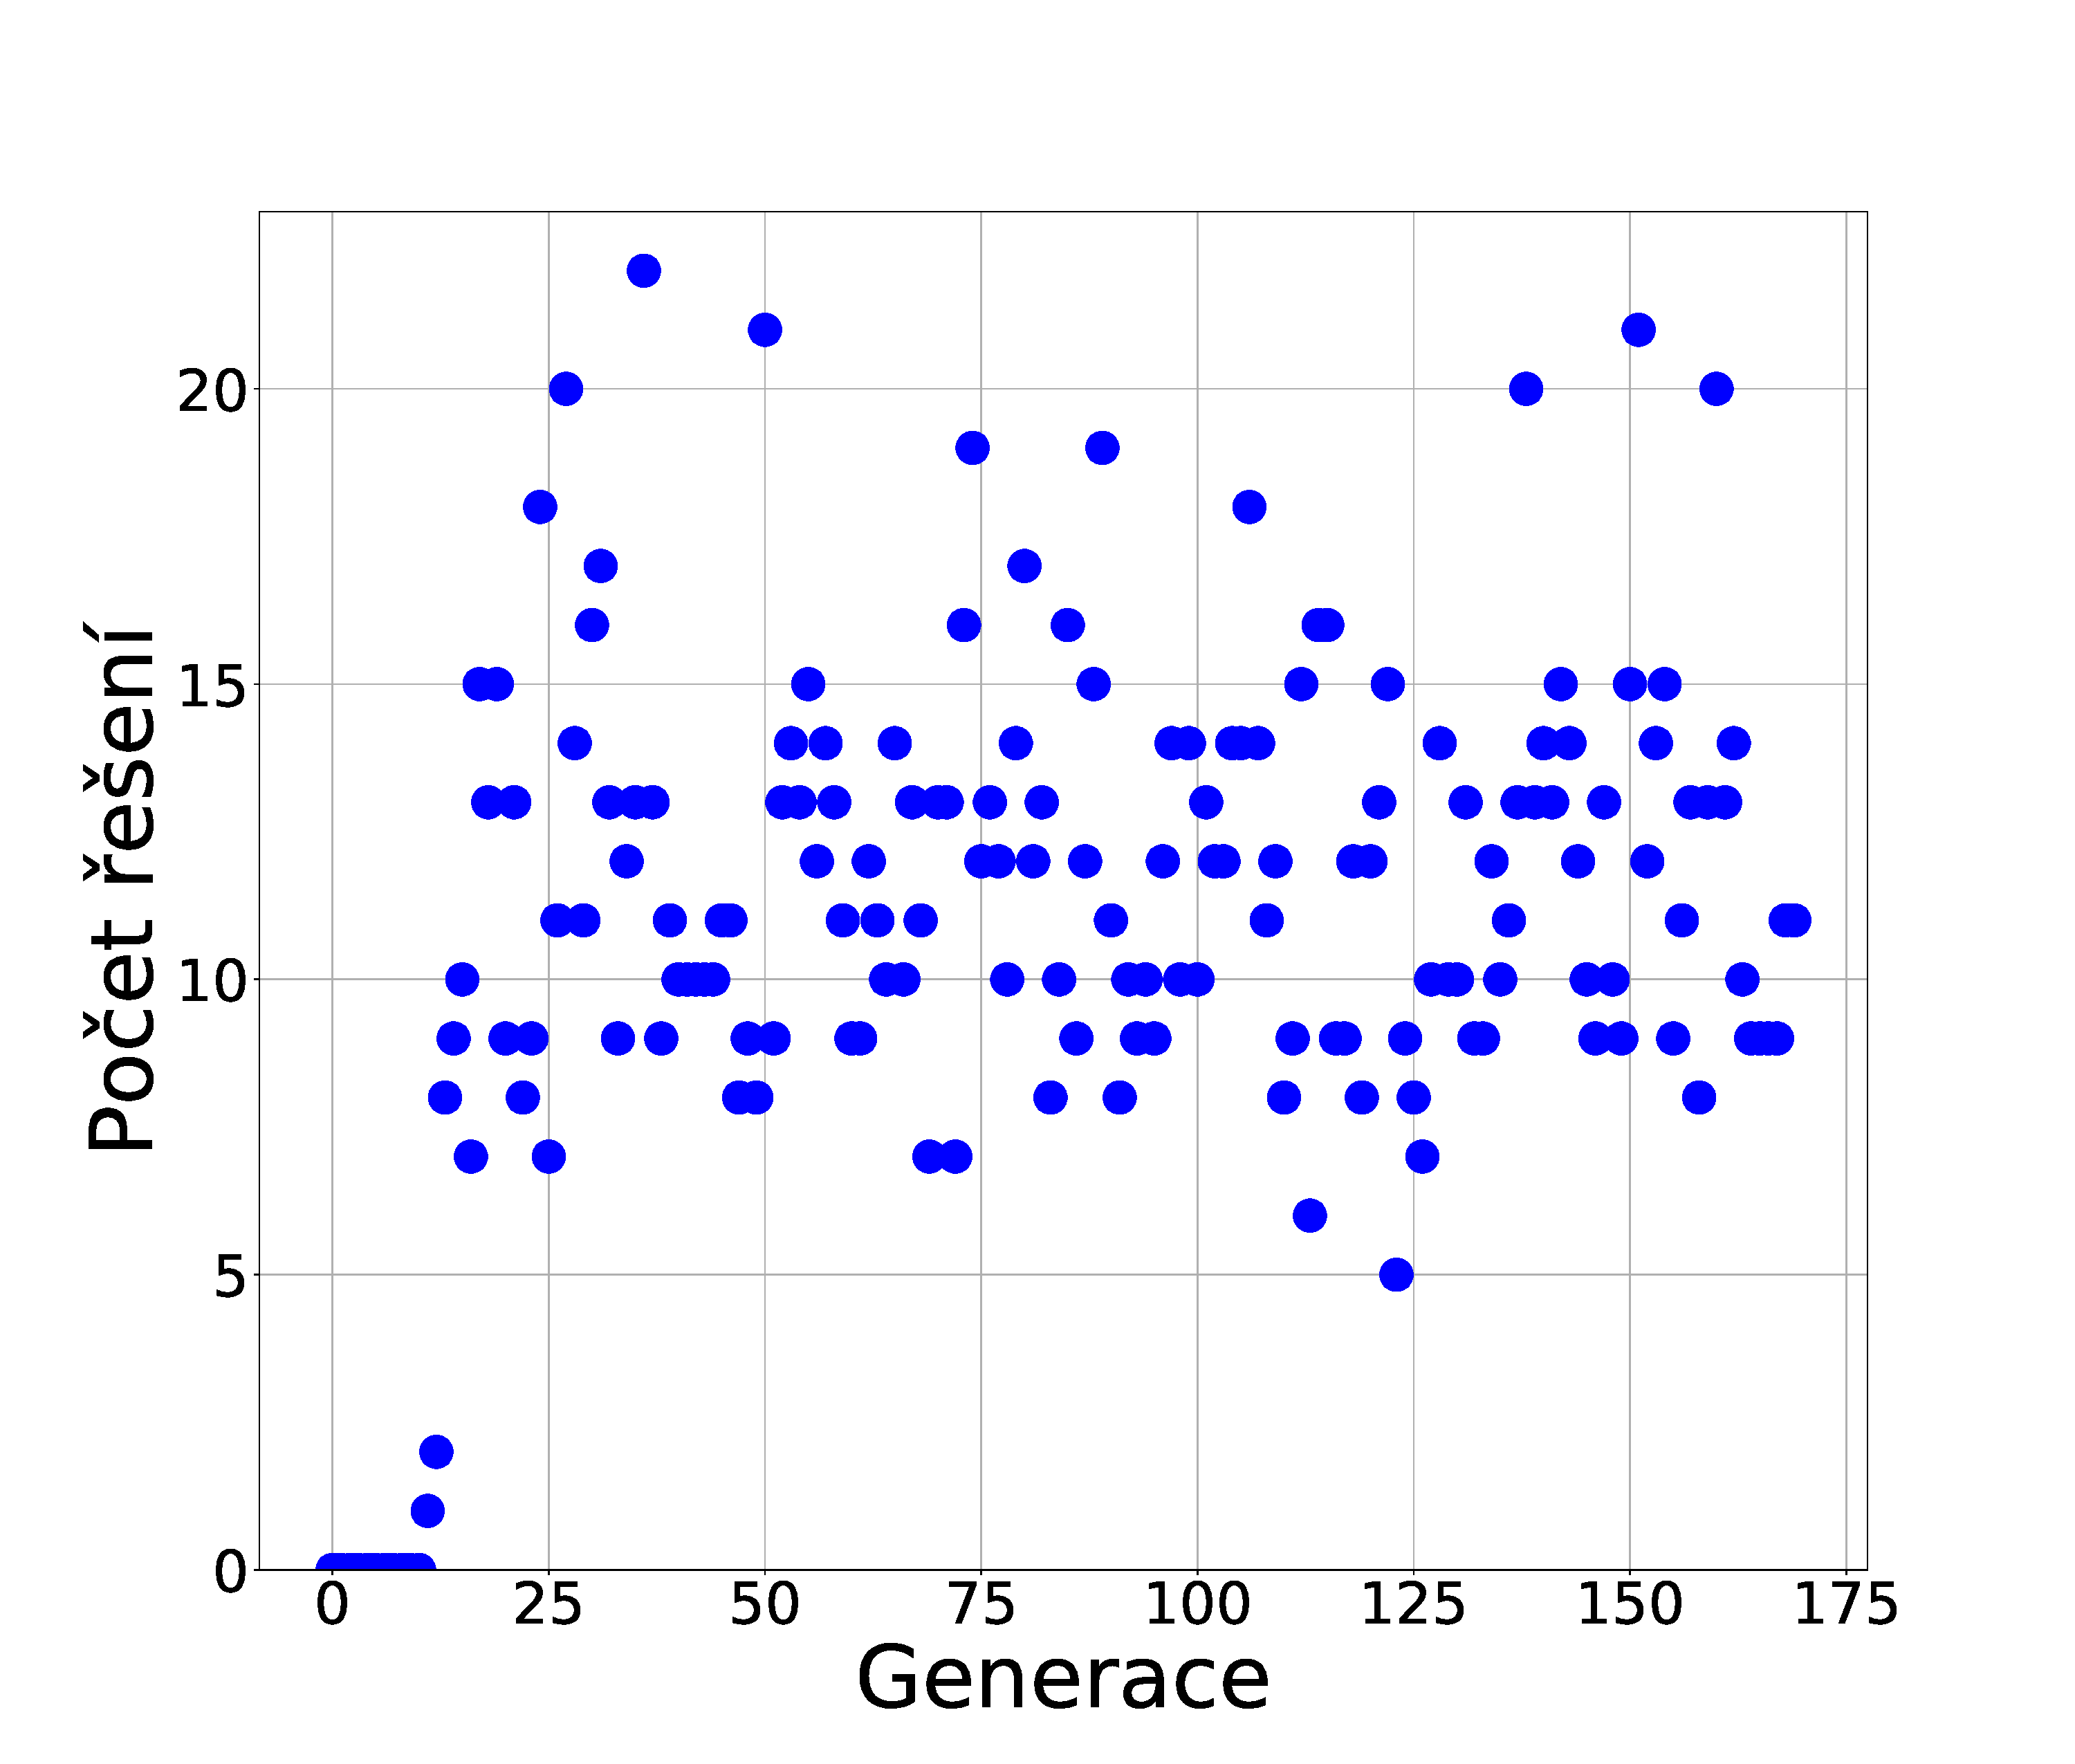
\includegraphics[width=\textwidth]{img/gc3s.pdf} 
    \end{minipage}
    \begin{minipage}[c]{0.325\textwidth}
        \centering 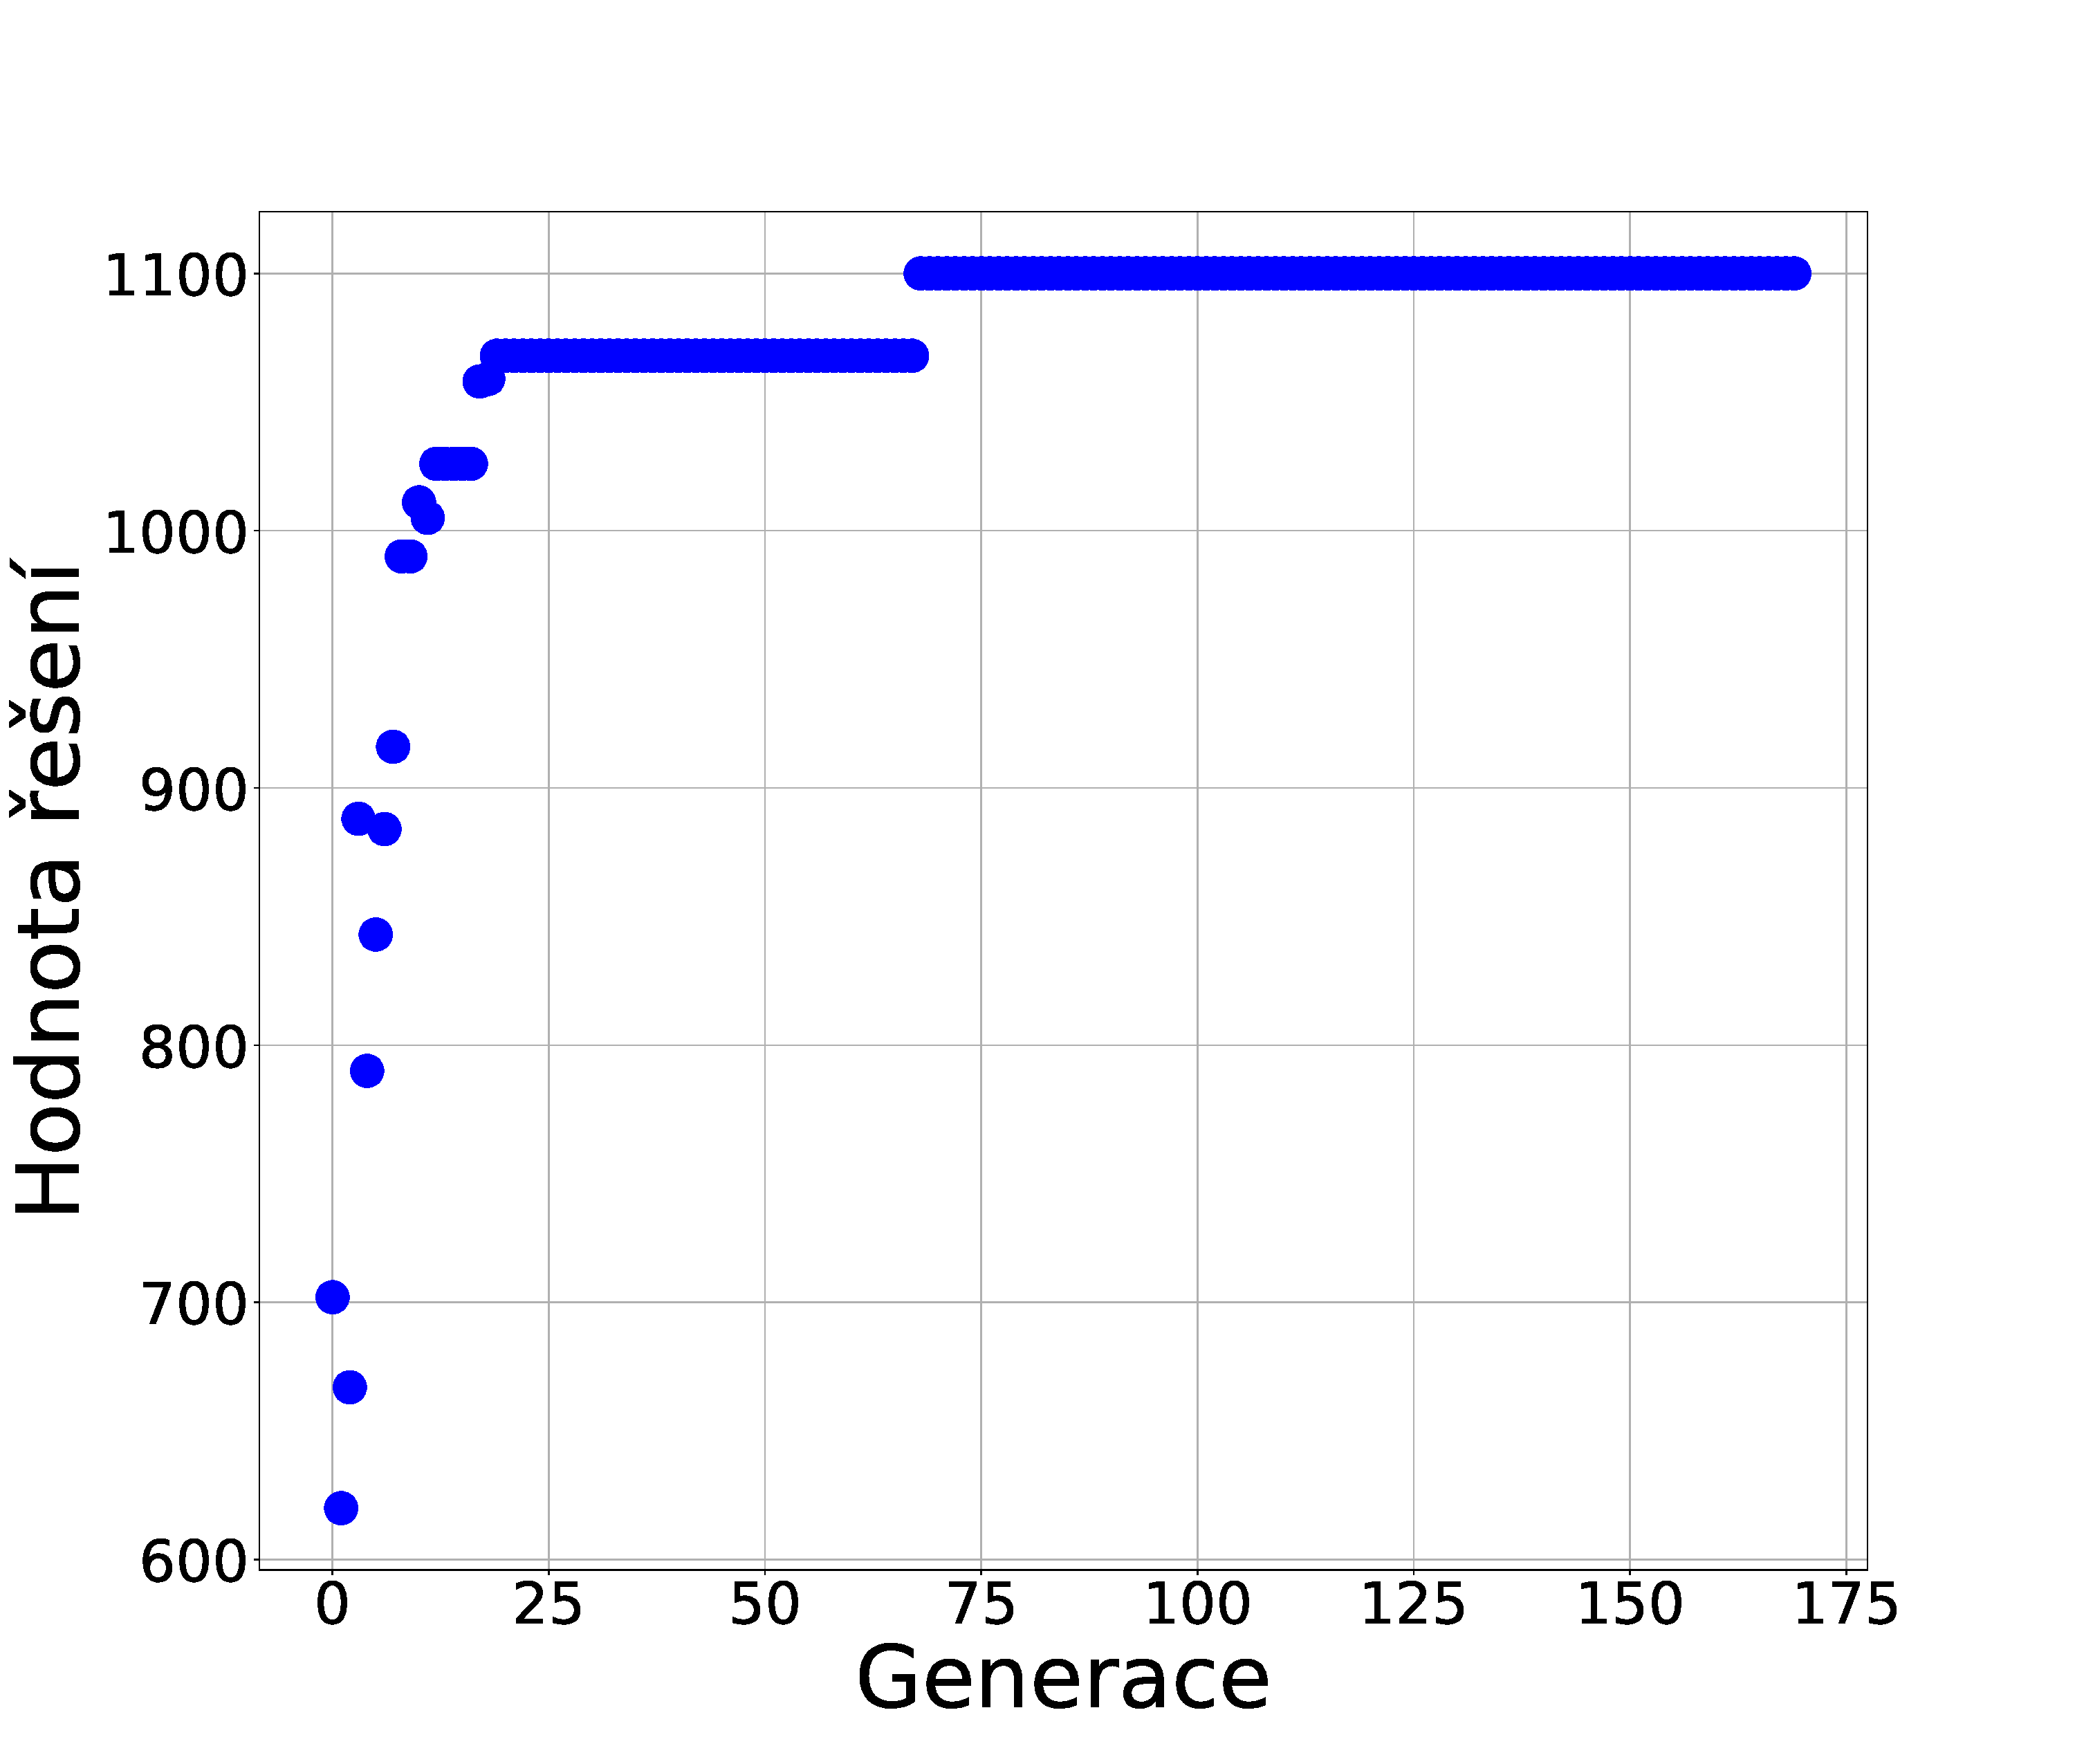
\includegraphics[width=\textwidth]{img/gc3w.pdf} 
    \end{minipage}
   \caption{Na tomto obrázku je nahoře uveden graf úspěšnosti v závislosti na cílovém počtu generací. Na grafech níže je průběh algoritmu pro různé počty generací. V levém sloupci jsou počty splněných klauzulí, uprostřed počet řešení a v pravém sploupci je hodnota výsledného řešení. (Na prvních třech grafech jsou na ose x desetiná čísla. Generace samozřejmě byla pouze celá čísla, toto je chyba u velmi nízkého počtu generací a čísla lze brát jako orientační.)}\label{fig:gencount}
\end{figure} 


\subsection{Závislost na počtu generací}
Na další parametr, na který jsem se zaměřil, je počet generací. Předpoklady v této kapitole byli jasné. S počtem generací roste i množství prozkoumaných řešení. Ty se, ale s velikým množství generací již mohou opakovat a proto by byla jen neuměrně navýšena doba běhu, ale na iterační sílu algoritmu by to již němelo vliv. 

Výsledky jsou zobrazeny na obrázku \ref{fig:gencount}. První graf je průměr při testování všech instancí. Grafy dole jsou ukázky běhu pro jednu vybranou instanci problému. Na prvním grafu je například vidět, že větší počet generací má větší vliv  na databázi D1, tedy problémy ze SATLIB. S dalším zvětšováním počtu generací se tento rozdíl tak nezvyšuje, ale čas stále narůstá minimálně lineárně (záleží jestli je zvyšován selekční tlak). Jako základní velikost pro experimenty jsem zvolil hodnotu 200. Z dat tohoto experimentu bych jako optimální počet generací volil 400 i přes vyšší časovou náročnost. 

Na grafech ze třech běhů je vidět, že se s zvýšením generačního cyklu zvýšila i iterační síla. Zvlášt je to vidě na grafech vpravo na obrázku \ref{fig:gencount}. Kde se již pro počet generací 175 podařílo dosáhnout hodnoty 1100 oproti 800 dozažených při pouze 20 generacích. 

\begin{wrapfigure}{r}{0.55\textwidth}
\begin{center}
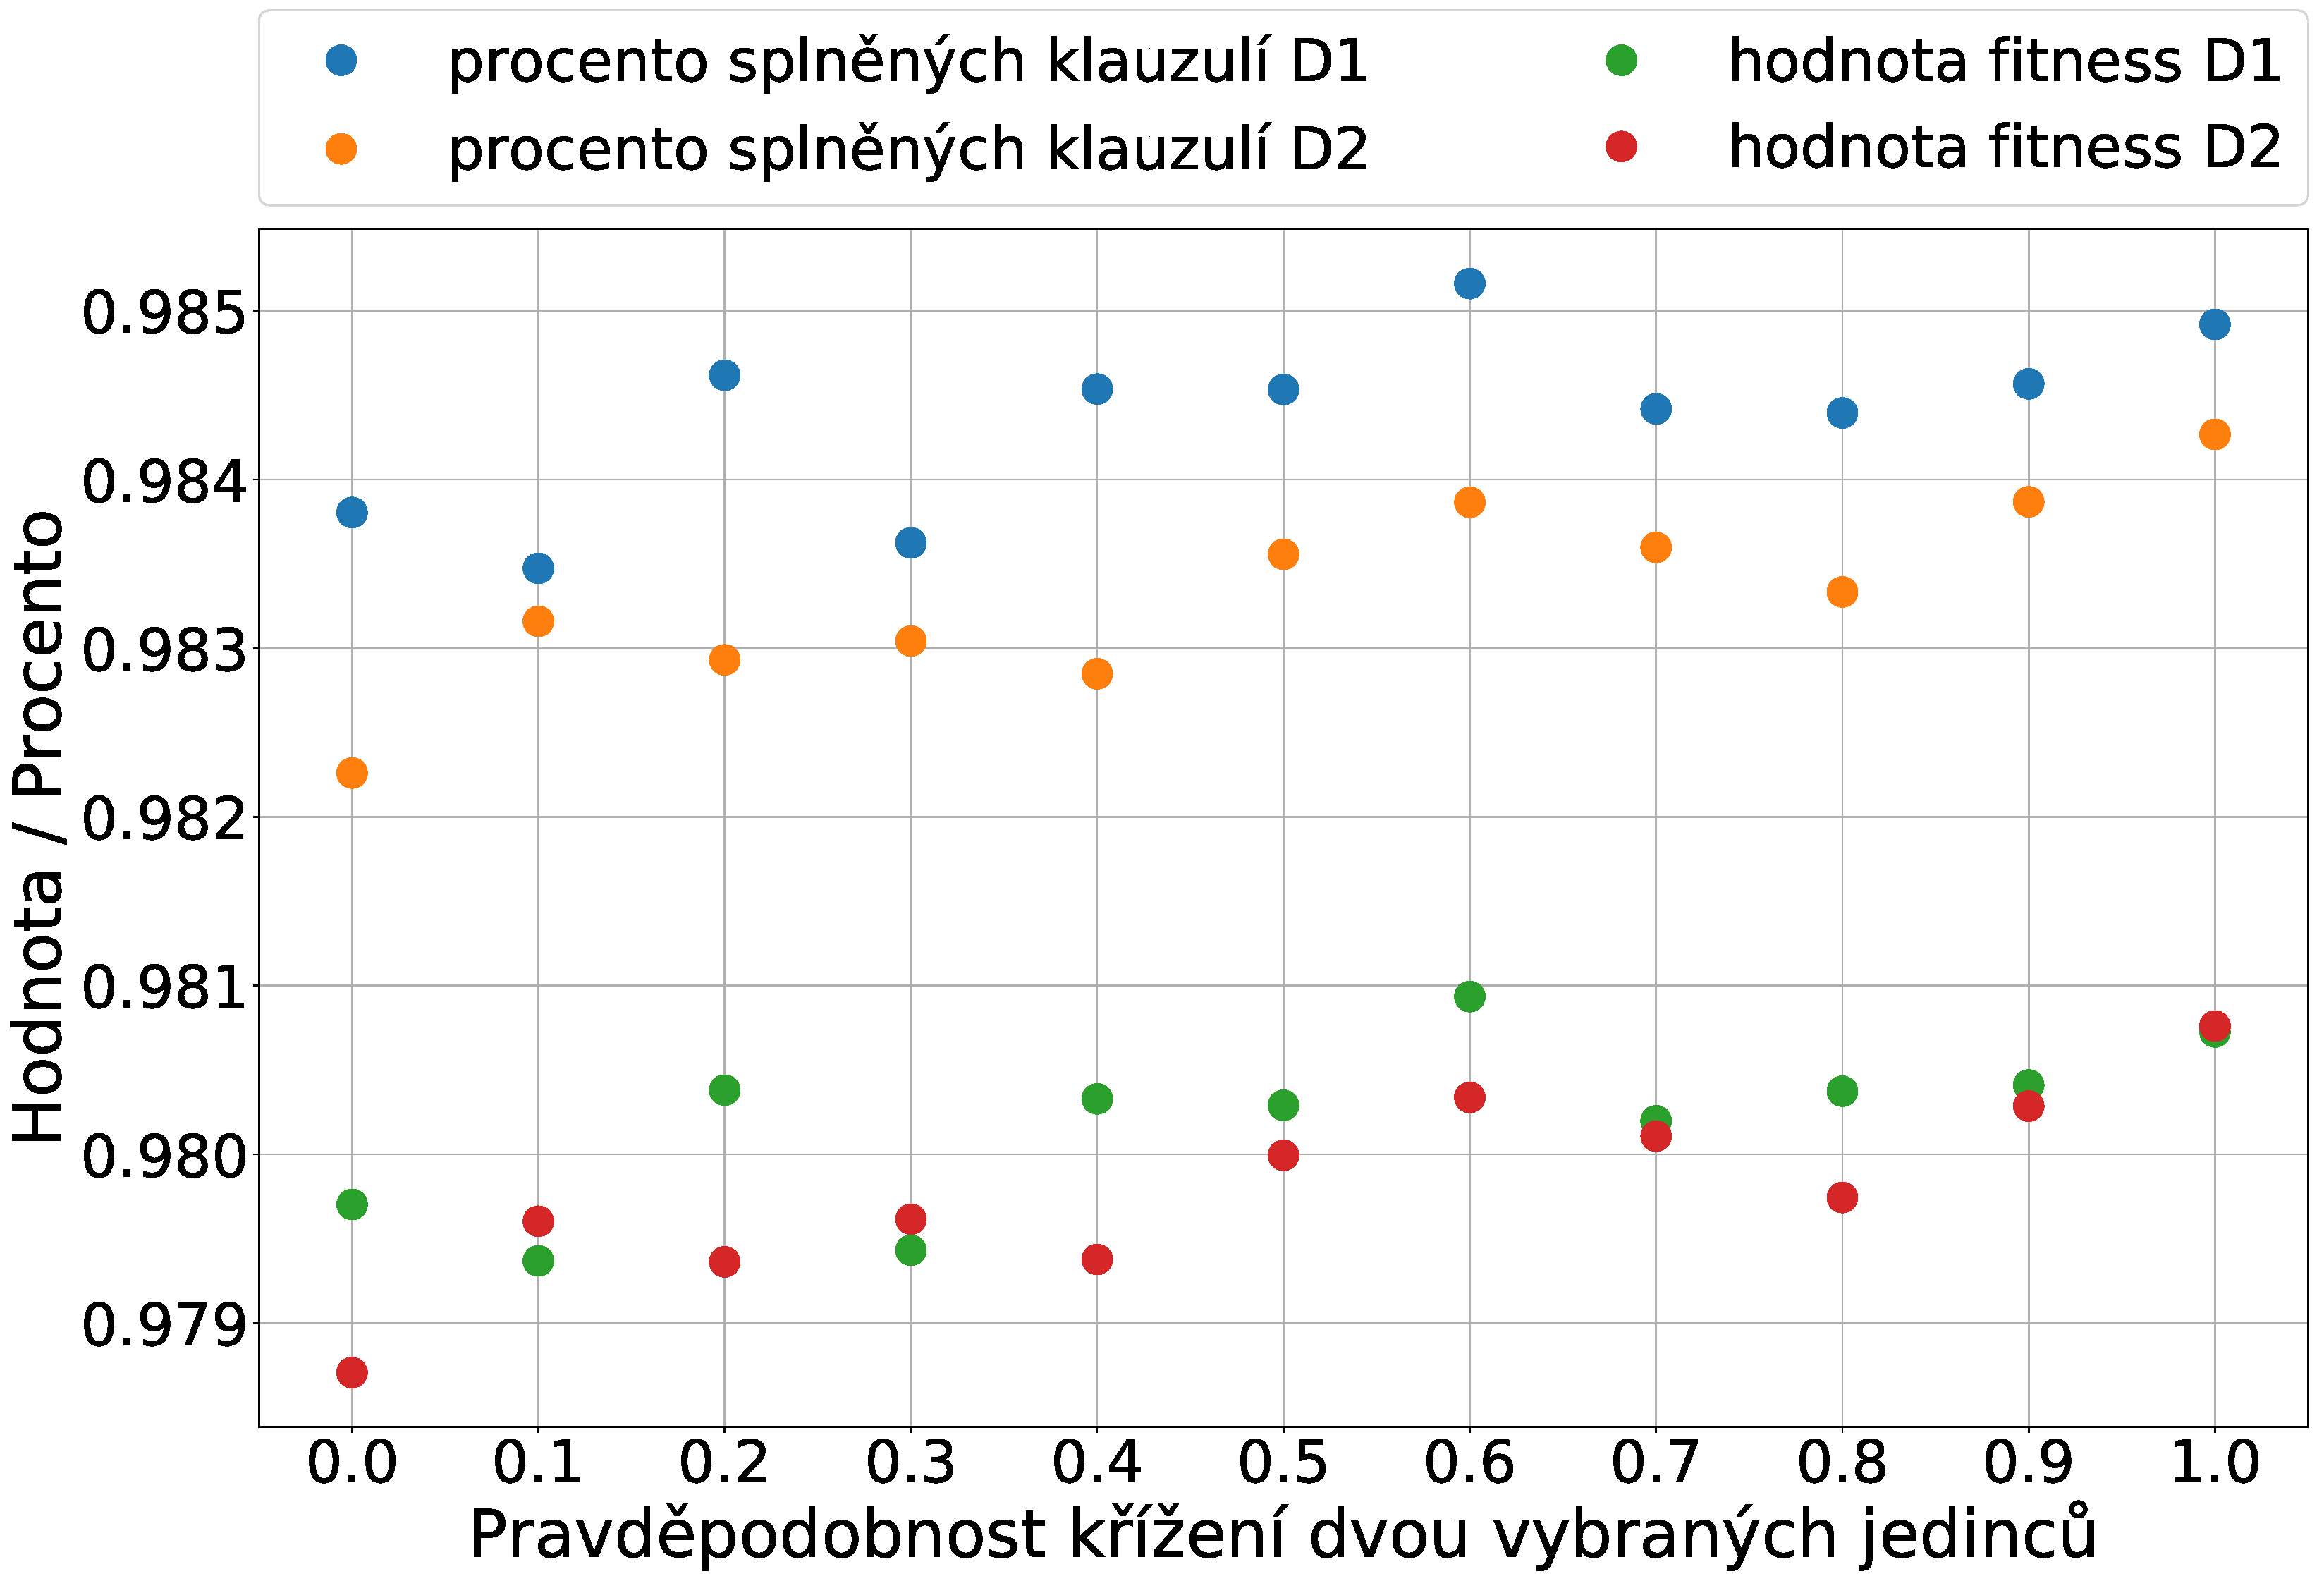
\includegraphics[width=0.55\textwidth]{img/sat_cross.pdf} 
\caption{Na obrázku je graf, kde je zobrazena úspěšnost v závislosti na pravděpodobnosti křížení.}
\label{fig:cross}
\end{center}
\end{wrapfigure}

\subsection{Závislost na pravděpodobnosti křížení vybraných jedinců}
Tento parametr jsem neodhadoval, ale pro základní nastavení jsem využil použití genetického algoritmu v jiném předmětu a~základní hodnotu nastavil na 0,7. Implementoval jsem dvě křížení a to uniformní a dvoubodové, kde jsem ve výsledku nakonec používál dvoubodové, které záchová větší časti genu pohromadě. Uniformní křížení by mohlo mít vliv jen náhodněho zámíchání dvou jedinců a jev by se mohl blížit mutaci. 

Z obrázku \ref{fig:cross} je patrné, že procento křížení nemá tak veliký vliv na úspěšnost při řešení vážené splnitelnosti booleovské formule. Avšak pro oba datasety se maximální úspěšnosti dosahuje pro hodnotu pravděpodobnosti křížení 0,6. Tedy pro nastavení při řešení, co největšího množství problémů, bych zvolil místo nastavení pravděpodobnosti křížení 0,7, hodnotu 0,6.

\begin{wrapfigure}{r}{0.55\textwidth}
\begin{center}
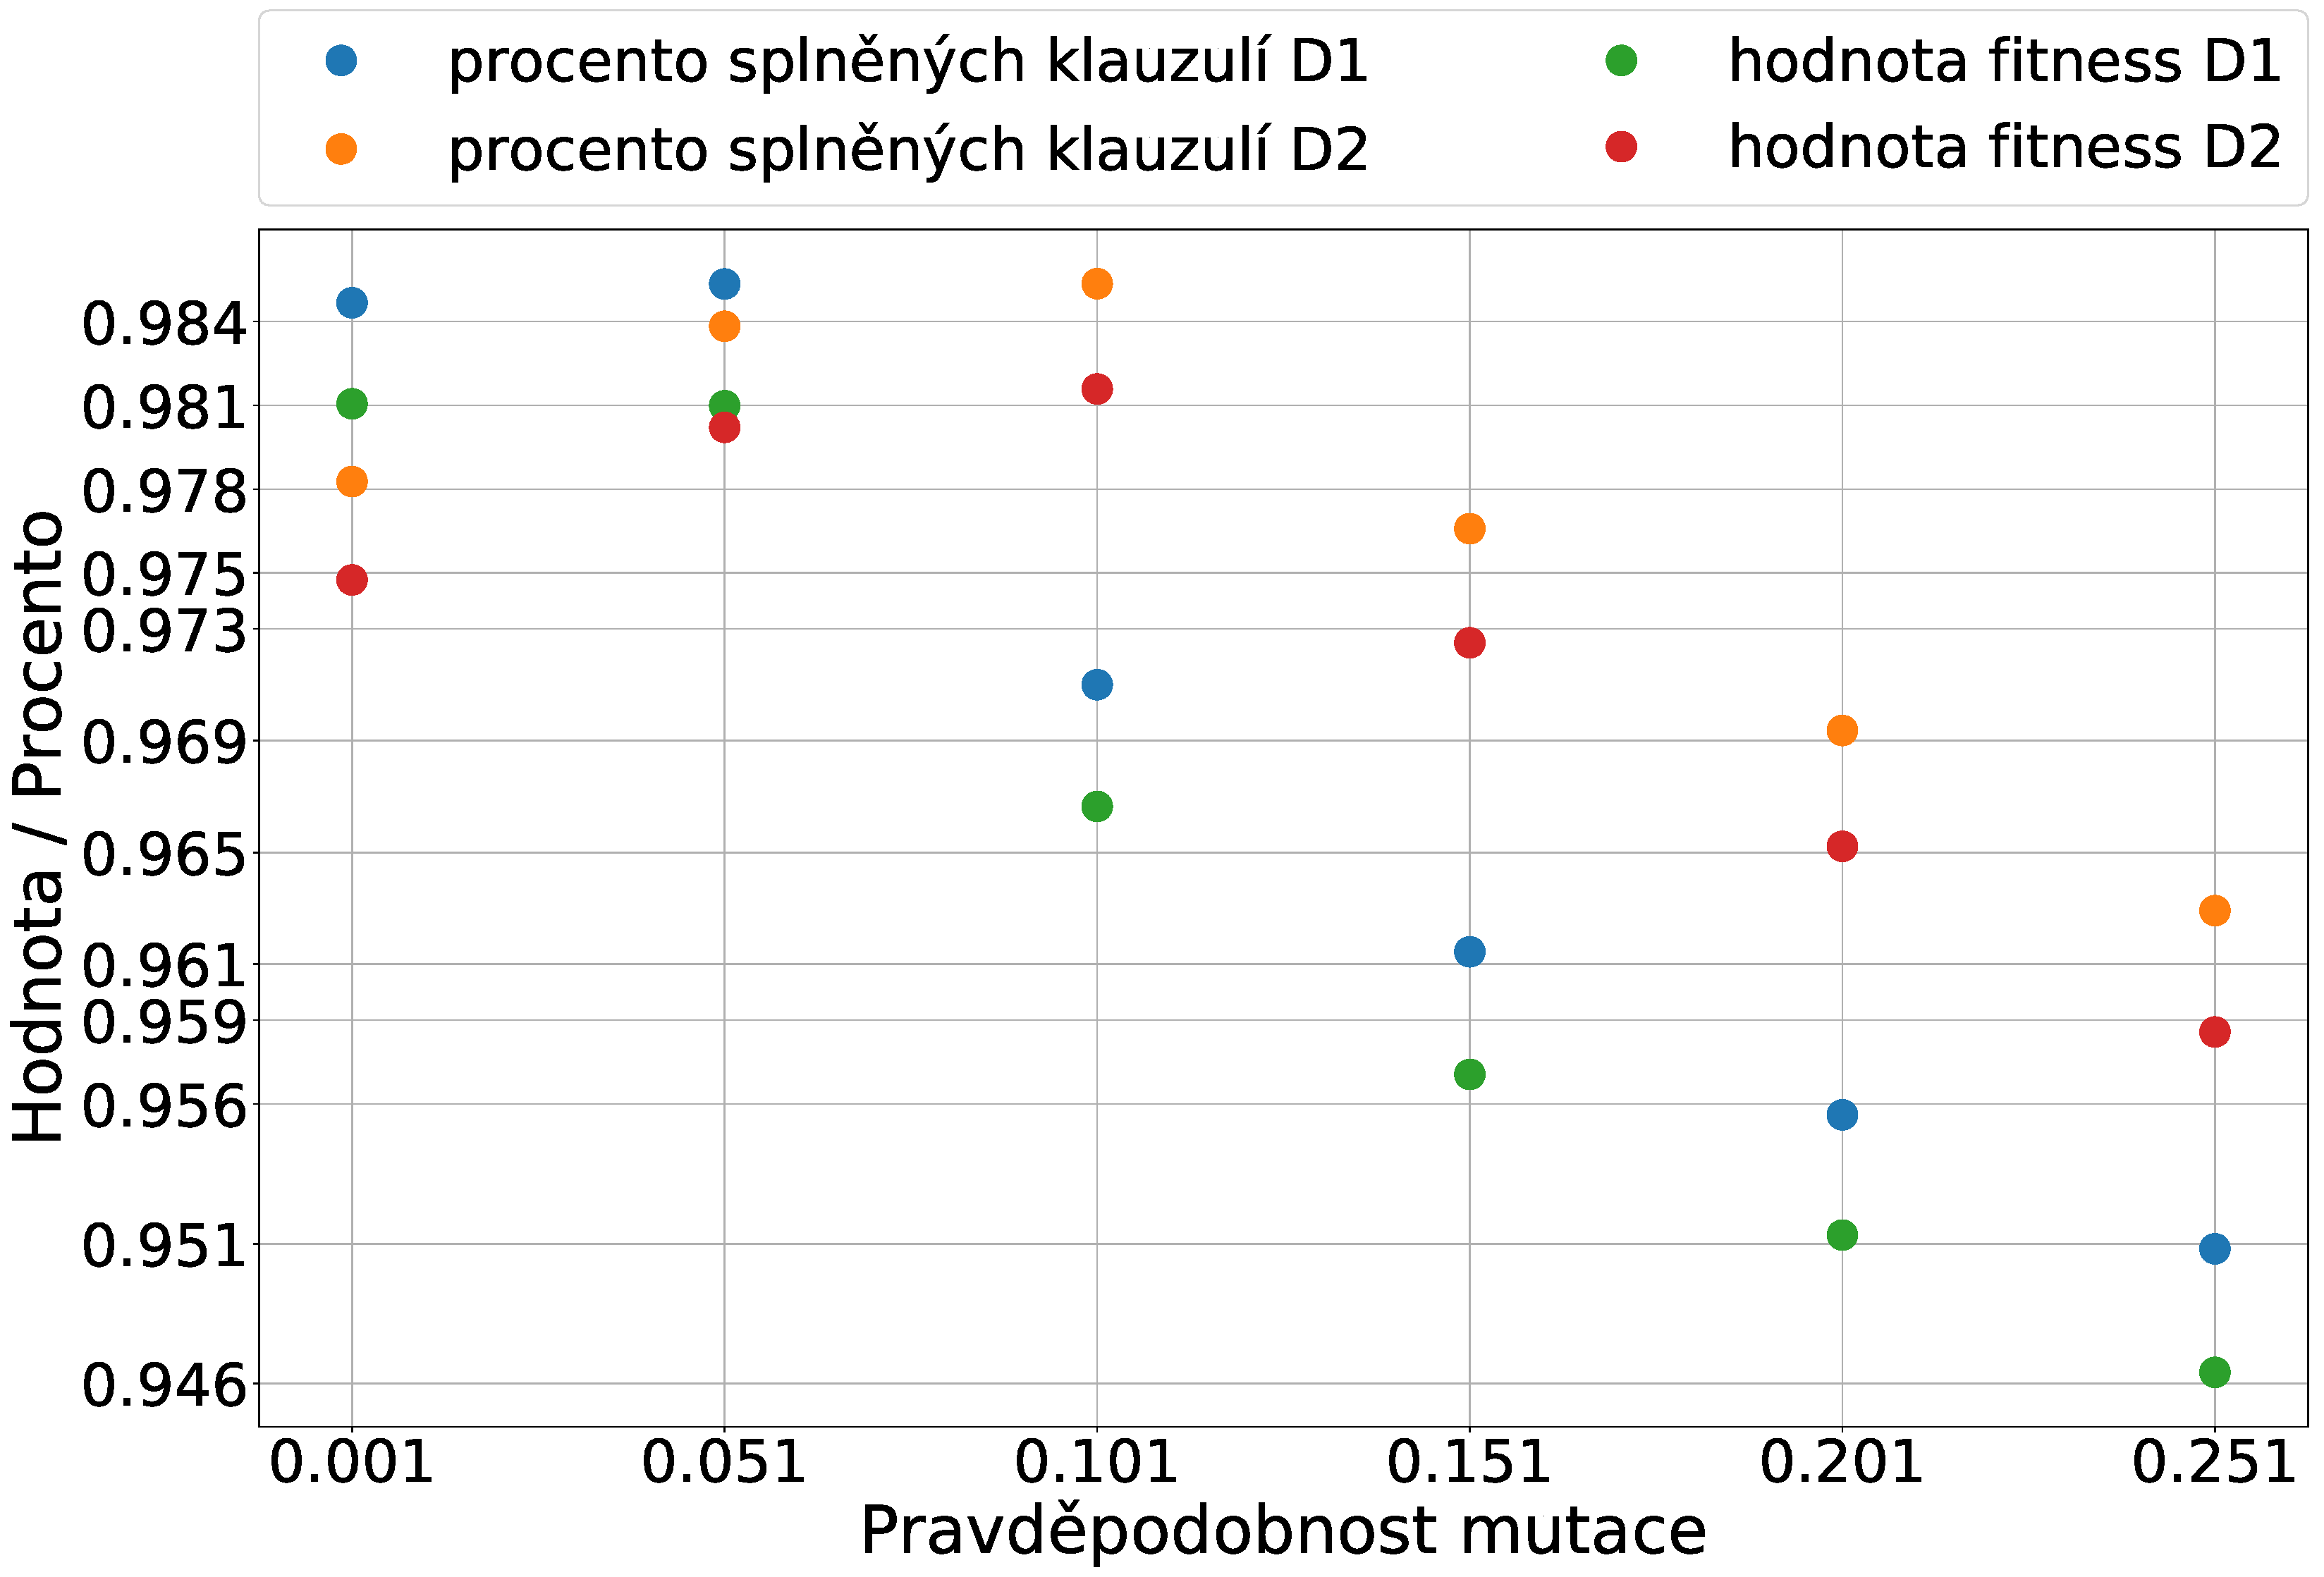
\includegraphics[width=0.55\textwidth]{img/sat_mut.pdf} 
\caption{Na obrázku je graf, kde je zobrazena úspěšnost v závislosti na pravděpodobnosti mutace.}
\label{fig:mut}
\end{center}
\end{wrapfigure}

\subsection{Závislost na pravděpodobnosti mutace}
U tohoto parametru jsem odhadoval, že bude určitě existovat hranice, do které se bude úspěšnost algoritmu zlepšovat, neboť bude mít mutace pozitivní vlik na diverzifikaci populace. Avšak za nějakou hraniční hodnotou, potom mutace způsobí, že populace nebude směřovat k lepším řešením, ale bude to náhodná procházka prostorem s diverzifikovanou populací, které se ovšem i tak může podařit nalézt řešení, neboť genetický algoritmus je randomizovaný.

Na obrázku \ref{fig:mut} jsou zobrazena data z~testování vlivu mutace. Předpoklad existence hranice, kde bude mutace ještě prospěšná, se potvrdil. Z grafu jde vidět, že ale tato hranice je pro každý dataset jiná. Toto může být způsobeno počtem proměných nebo poměrem klauzulí a počtu proměných. Tento jev a~zlom by bylo dobré při dalším testování více prozkoumat a pokusit se zachytit jeho závislosti. Podle grafu bych jako optimální hodnotu oproti zvolené 0,05 volil hodnotu asi jen o~malinko vyšší, tedy 0,06. 

\begin{landscape}
\begin{figure}
	\centering
    \begin{minipage}[c]{0.35\textwidth}
        \centering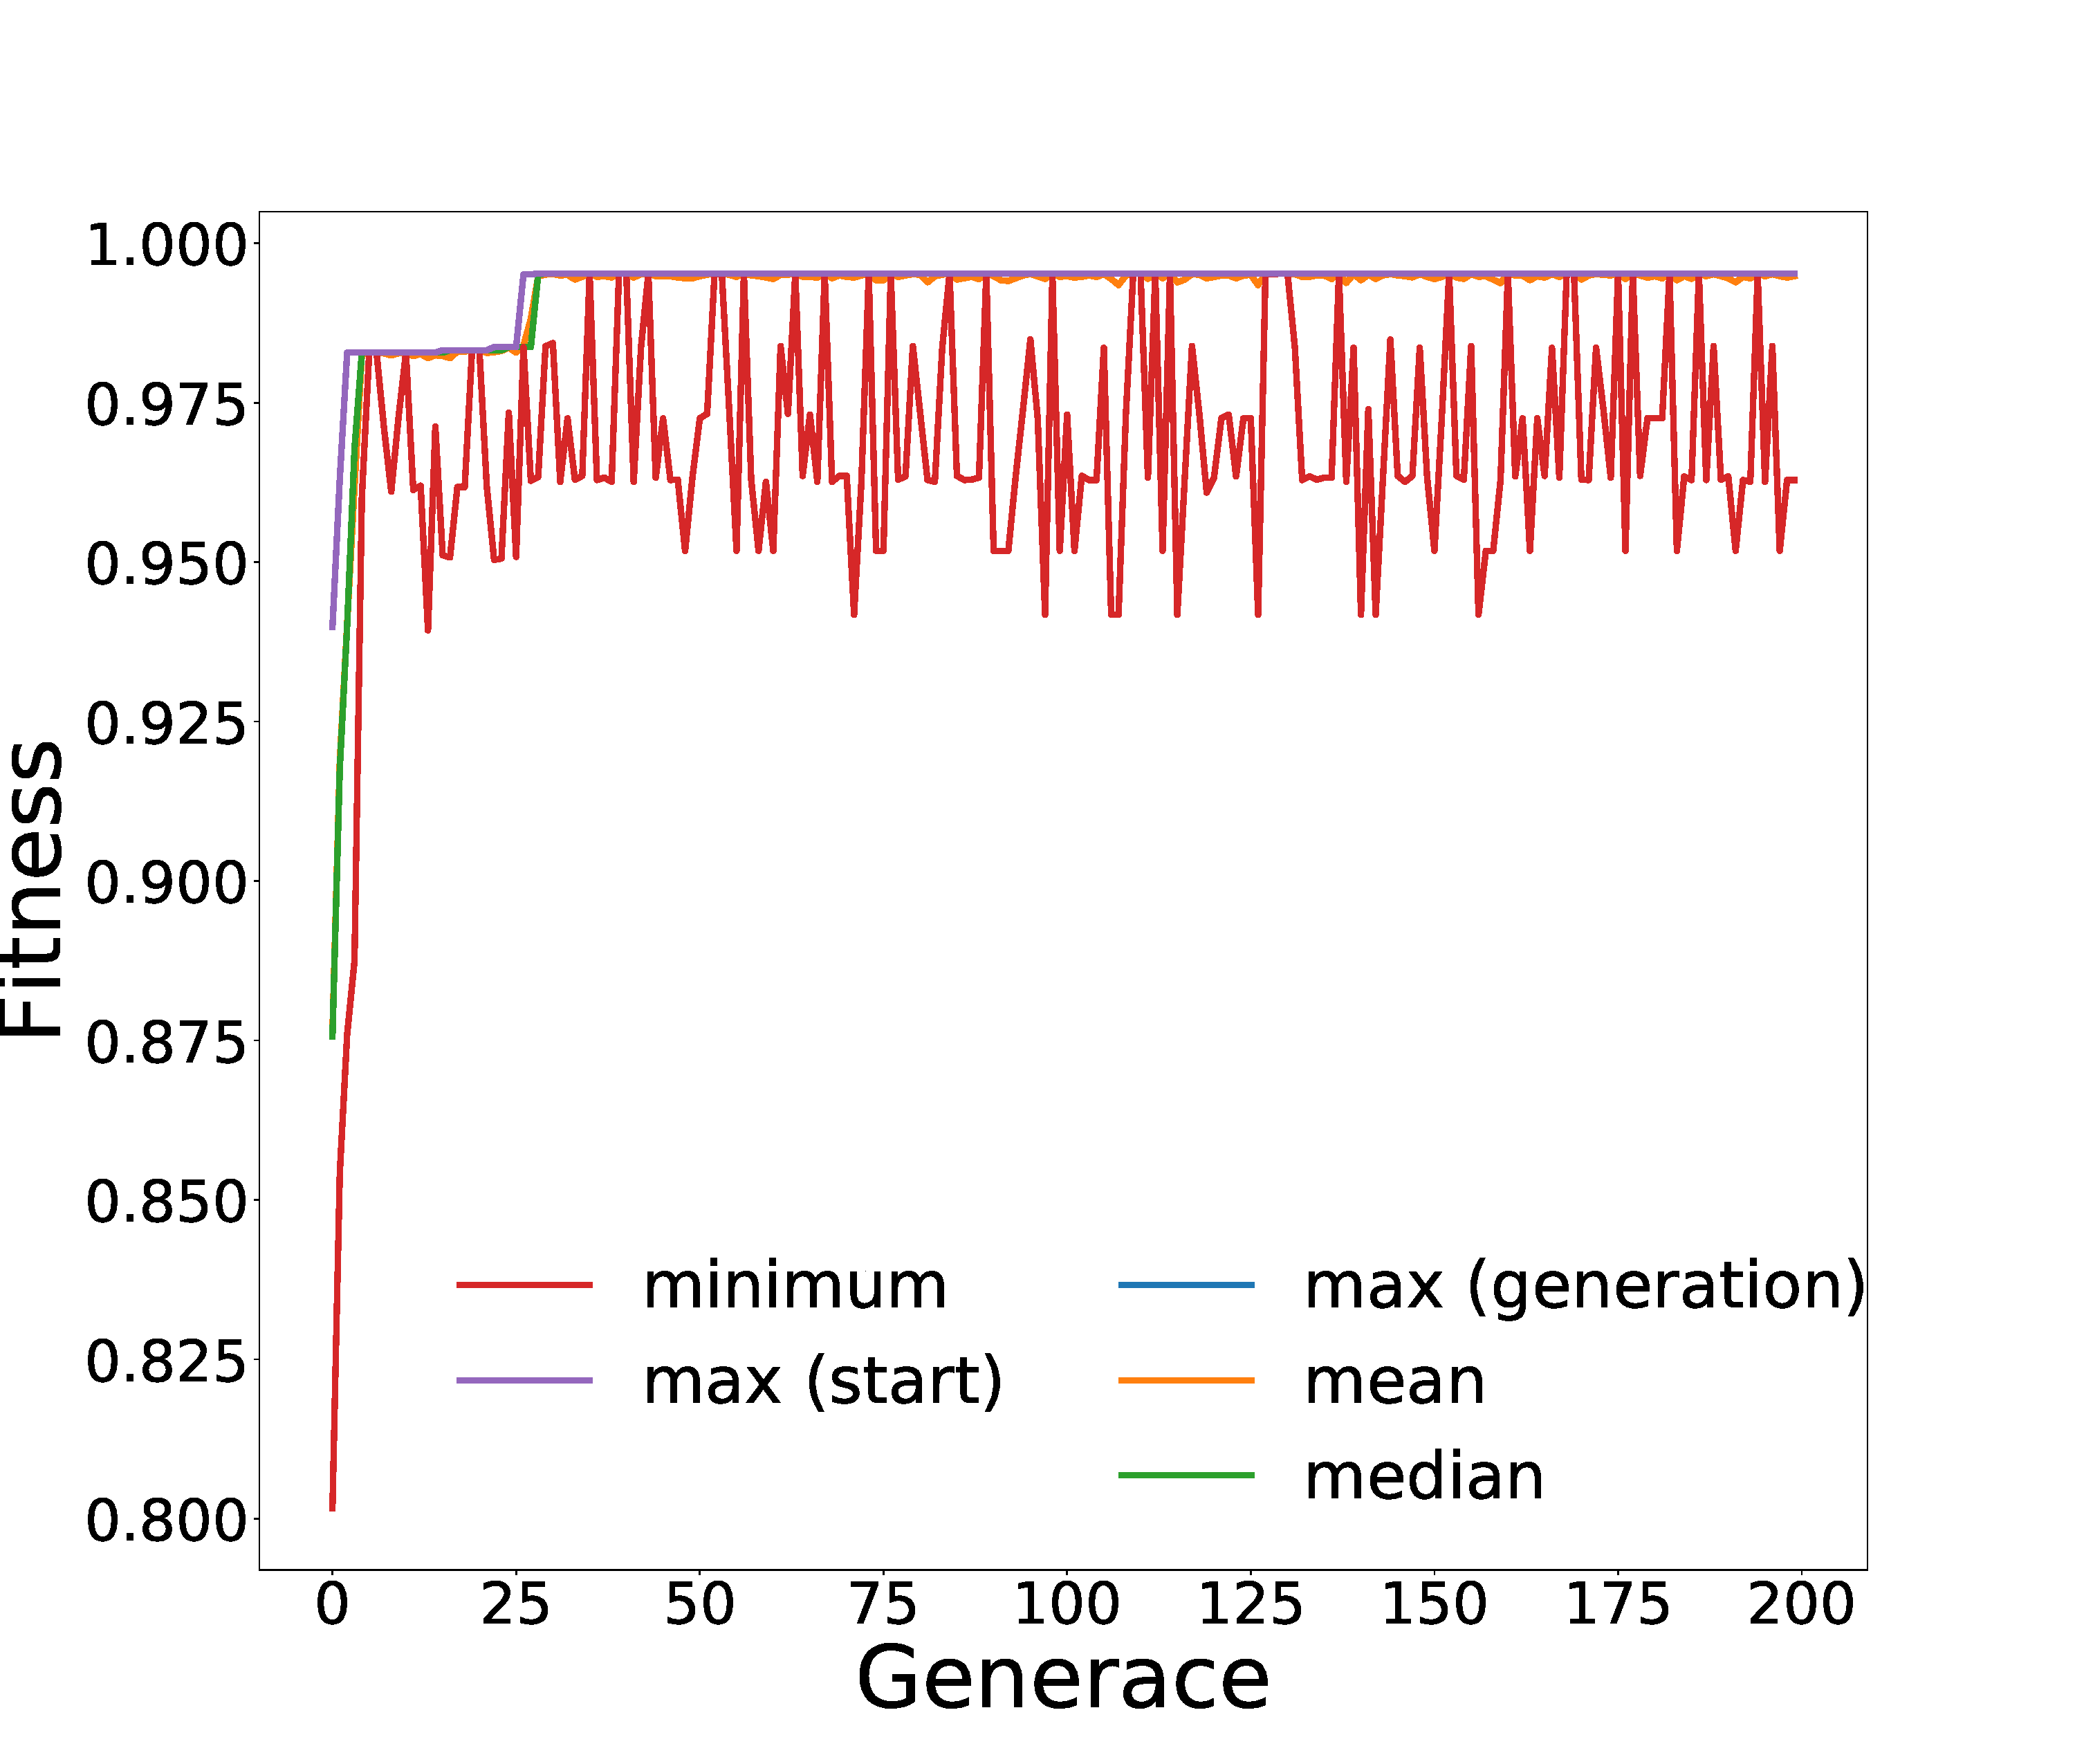
\includegraphics[width=\textwidth]{img/m001g.pdf} 
    \end{minipage}
    \begin{minipage}[c]{0.35\textwidth}
        \centering 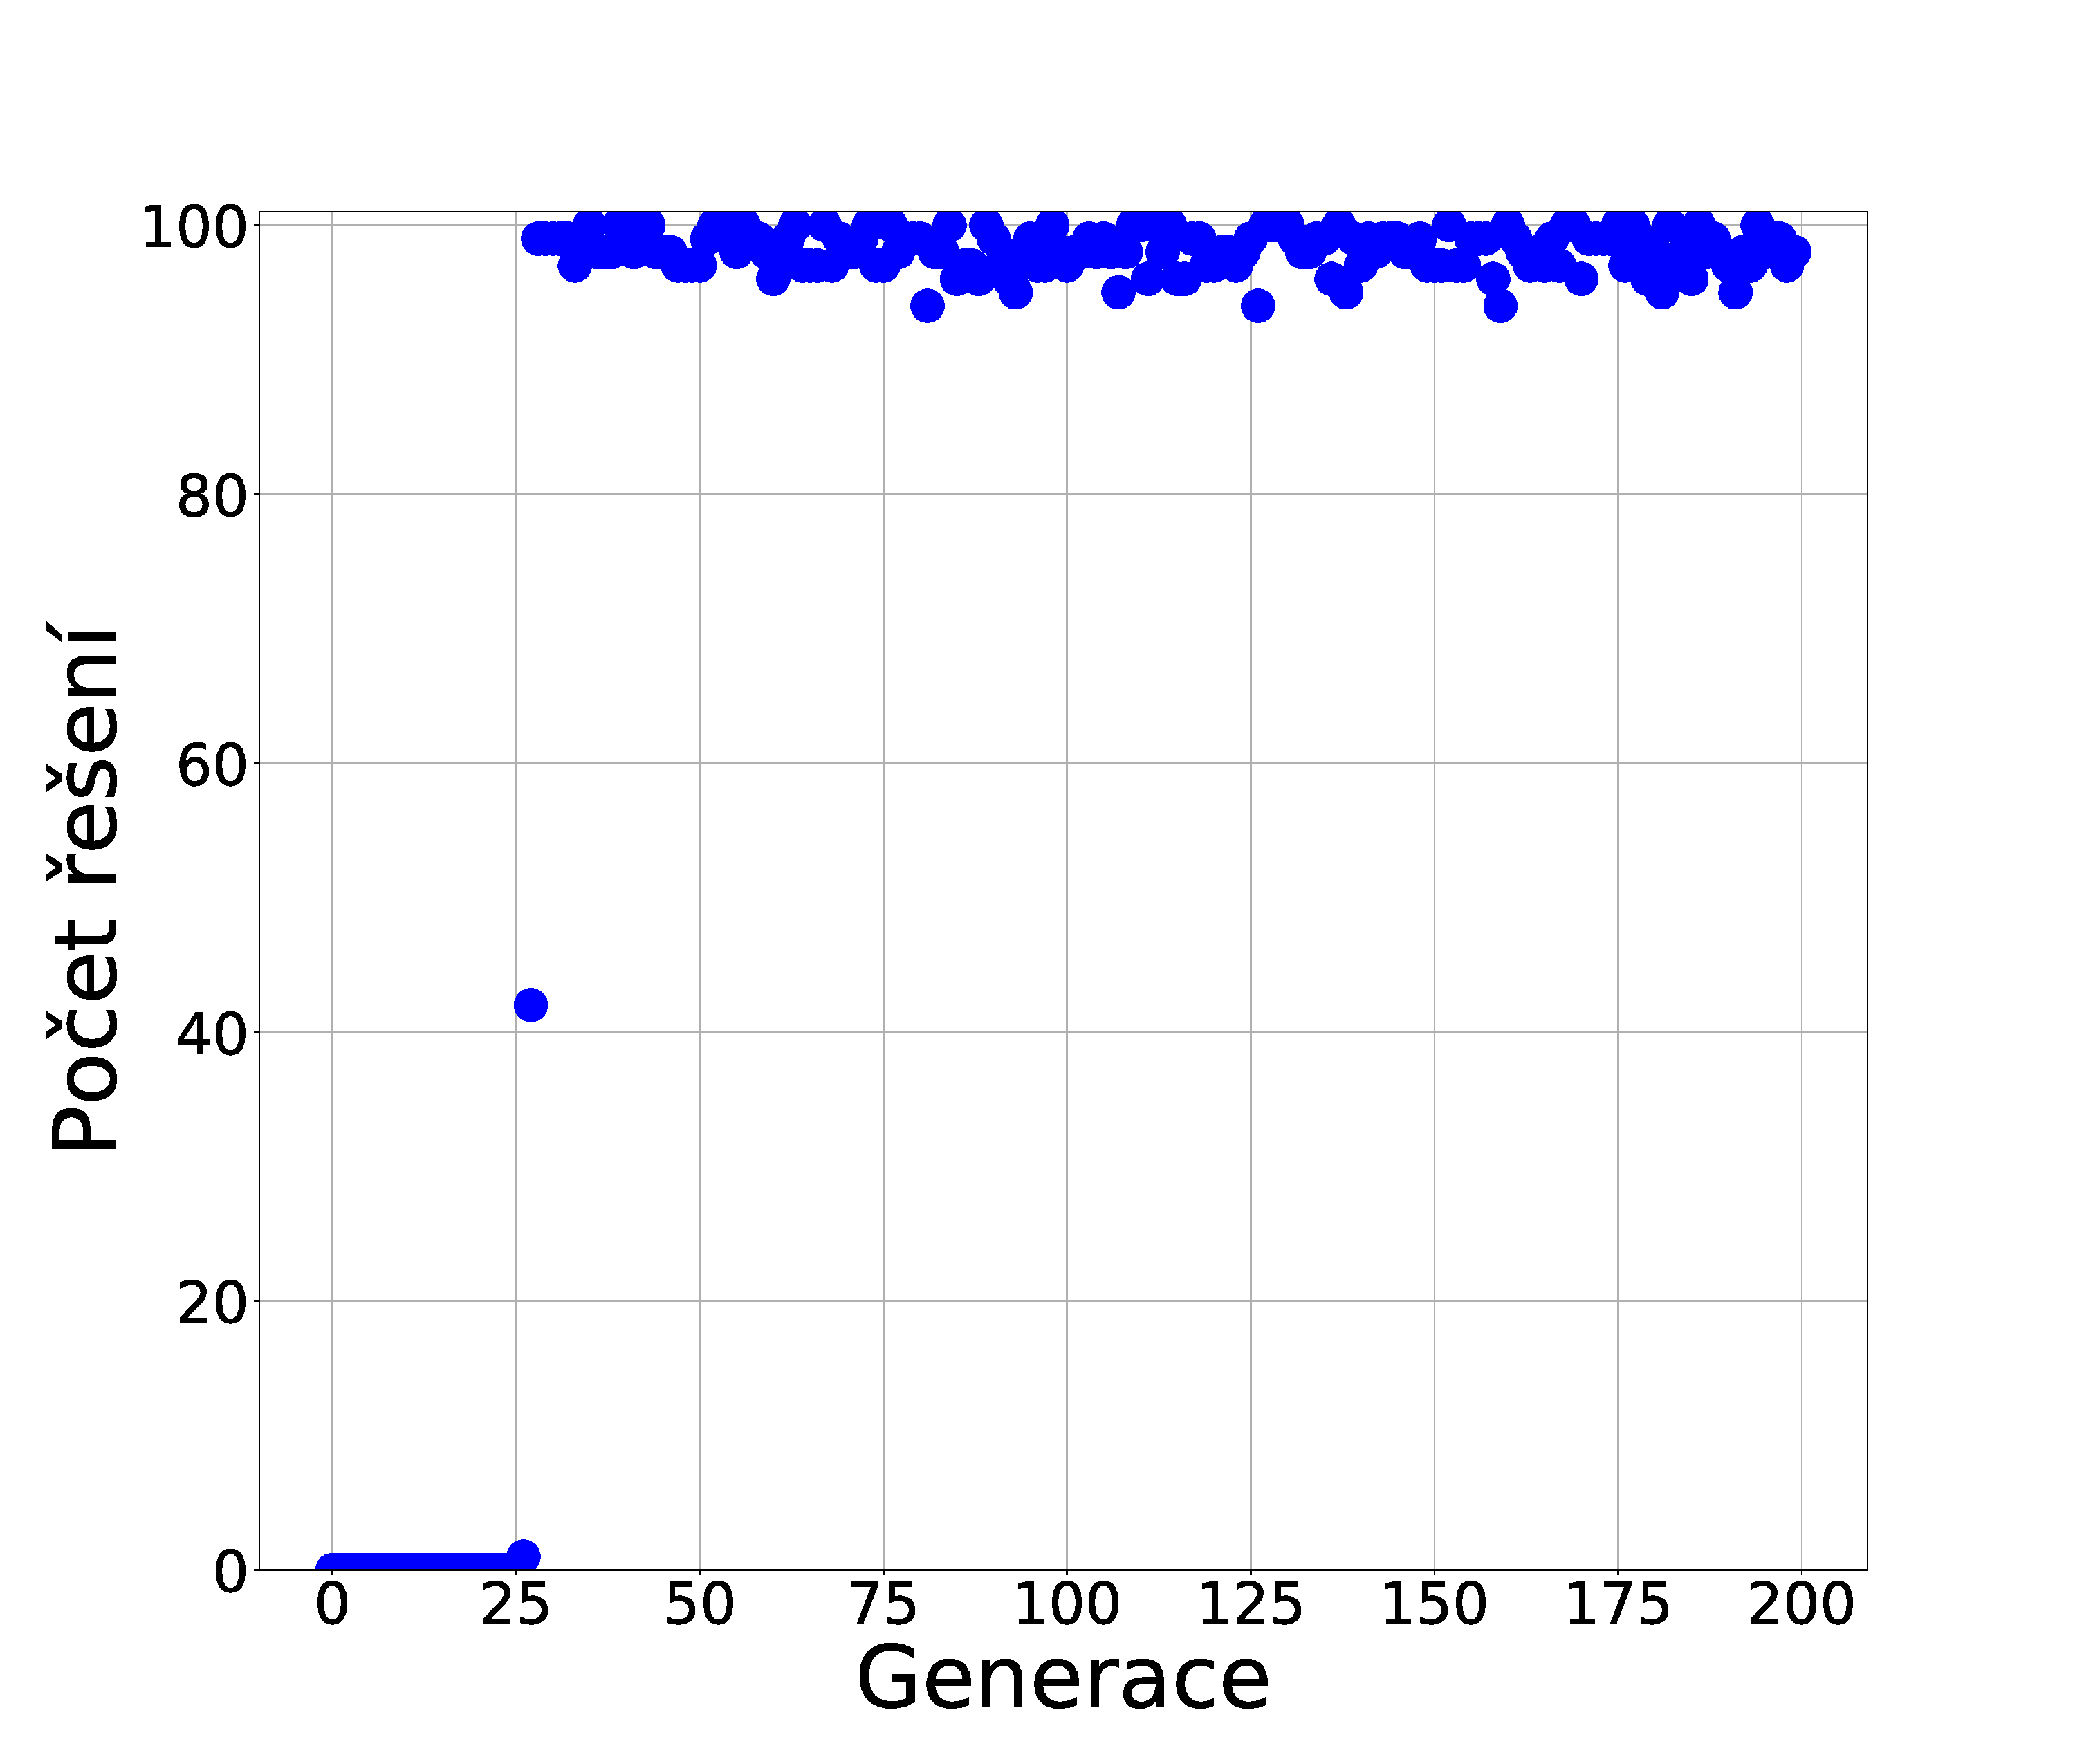
\includegraphics[width=\textwidth]{img/m001s.pdf} 
    \end{minipage}
    \begin{minipage}[c]{0.35\textwidth}
        \centering 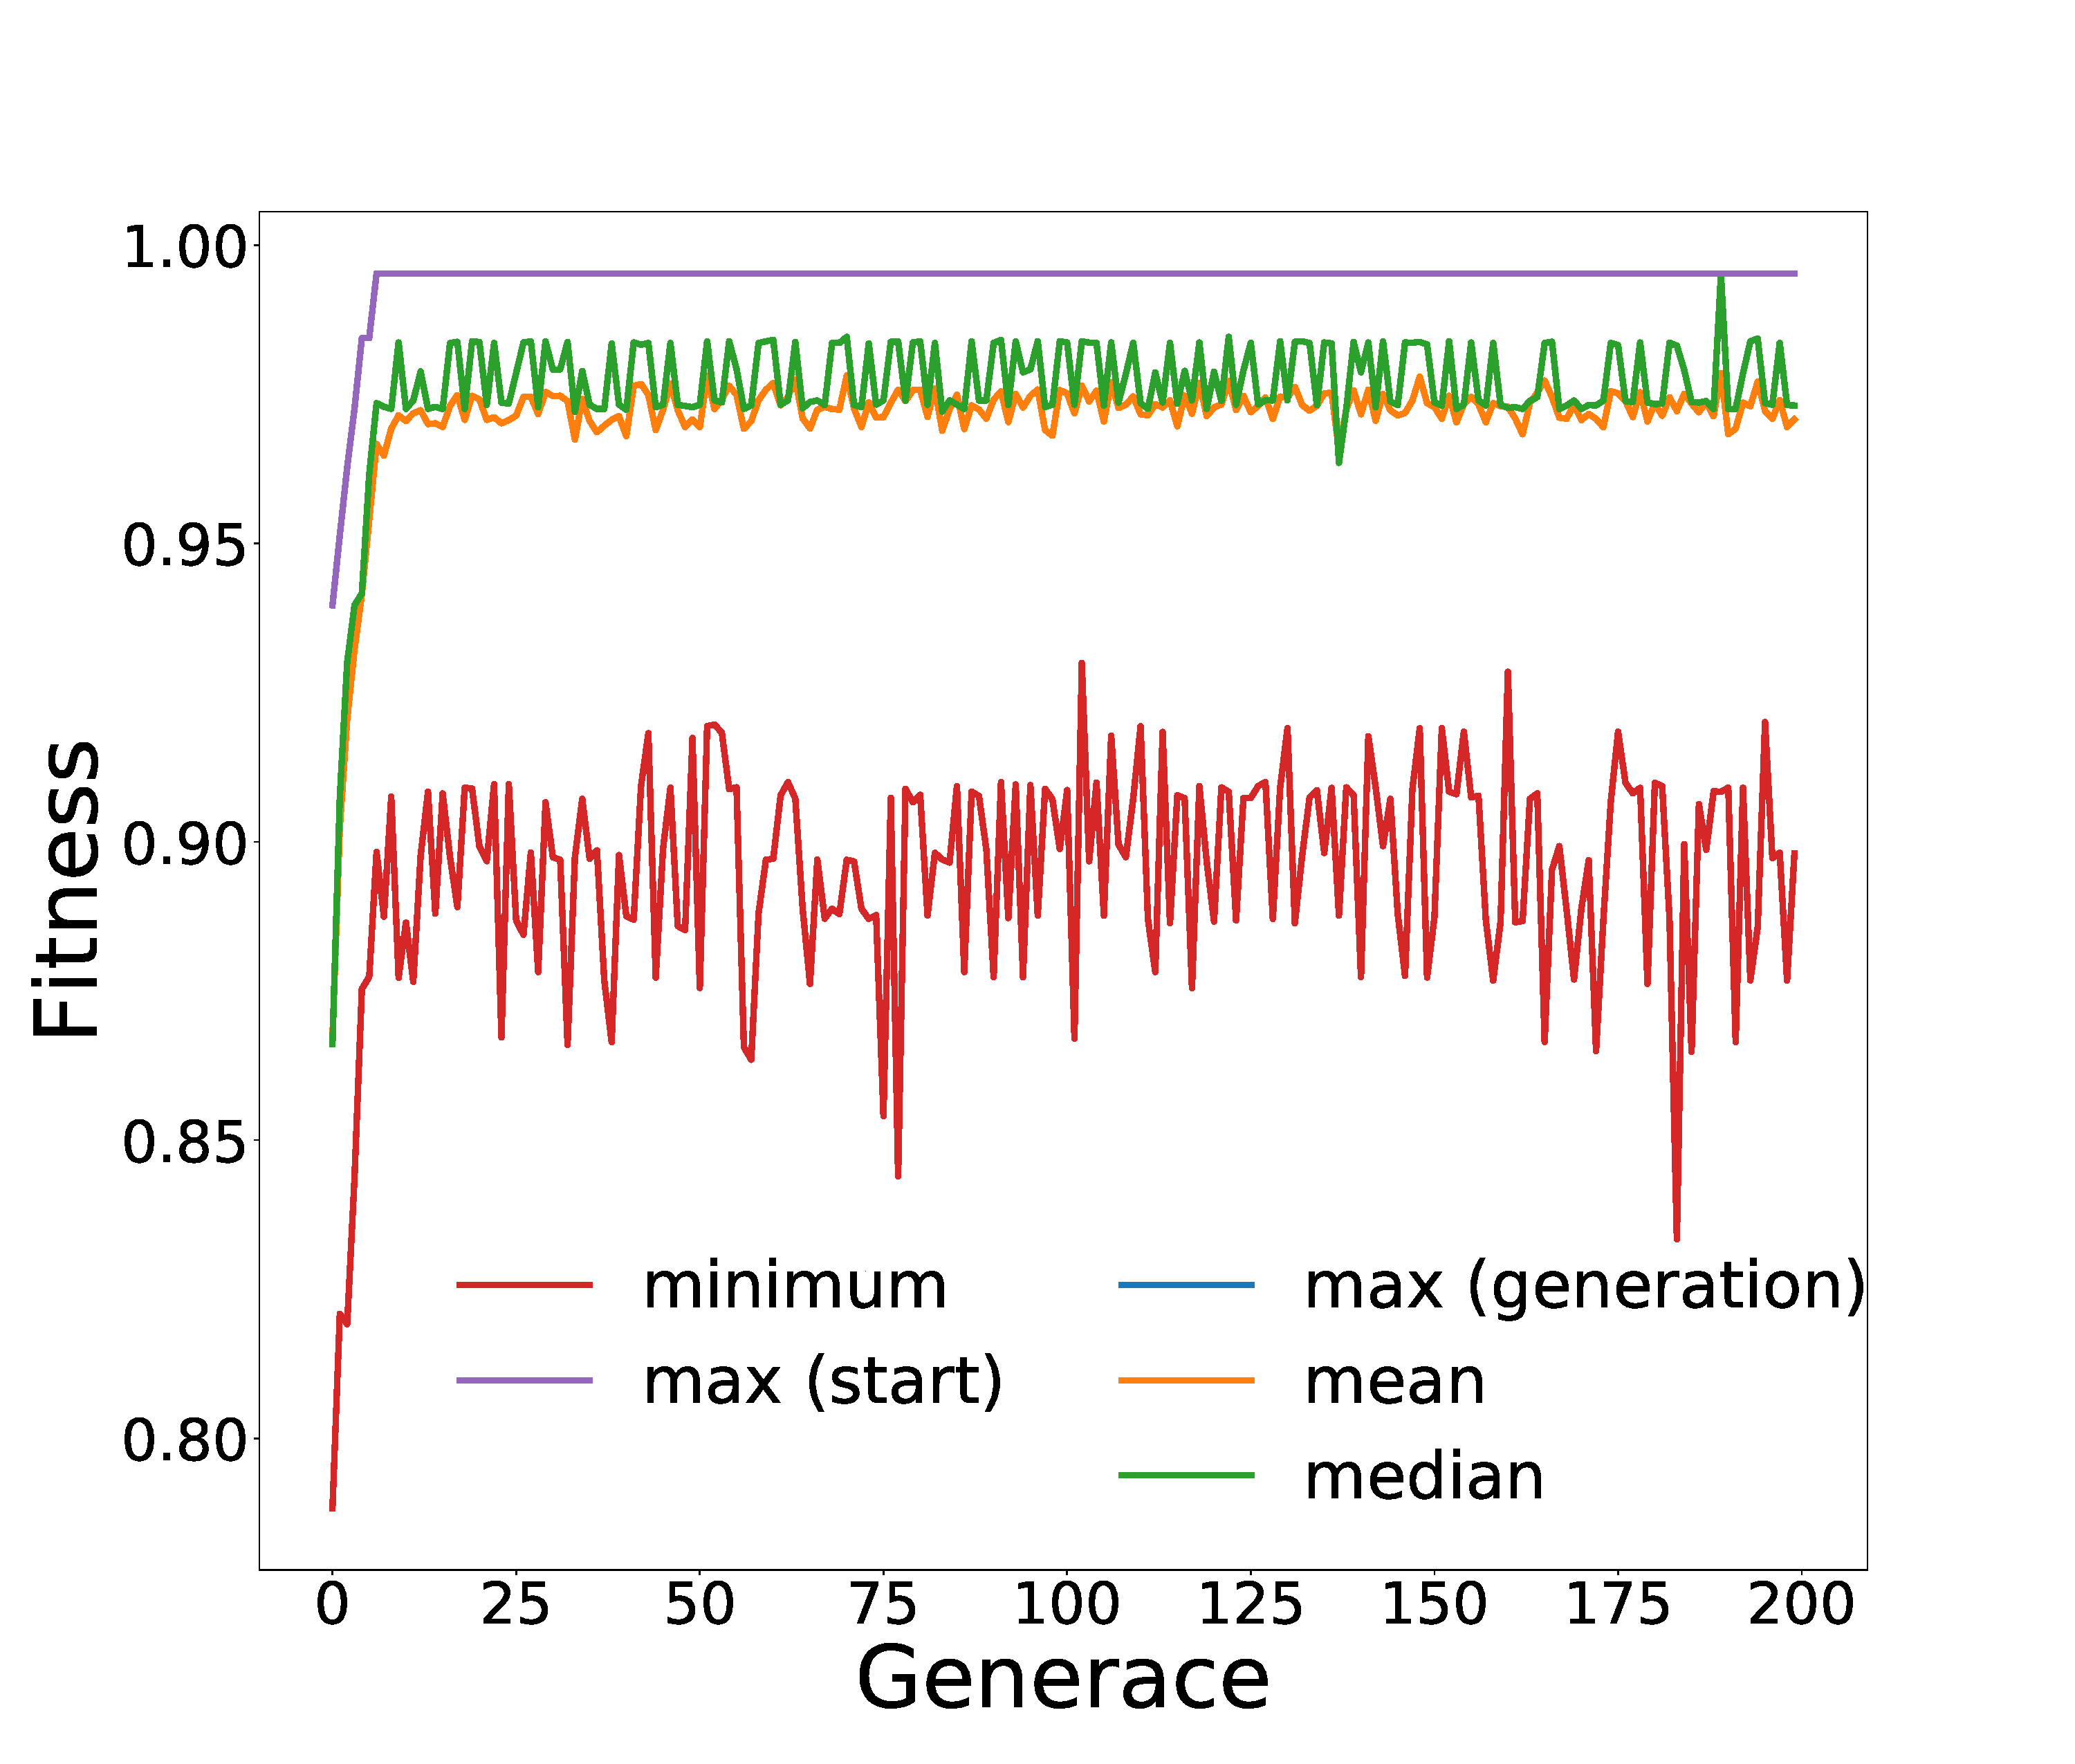
\includegraphics[width=\textwidth]{img/m051g.pdf} 
    \end{minipage}
    \begin{minipage}[c]{0.35\textwidth}
        \centering 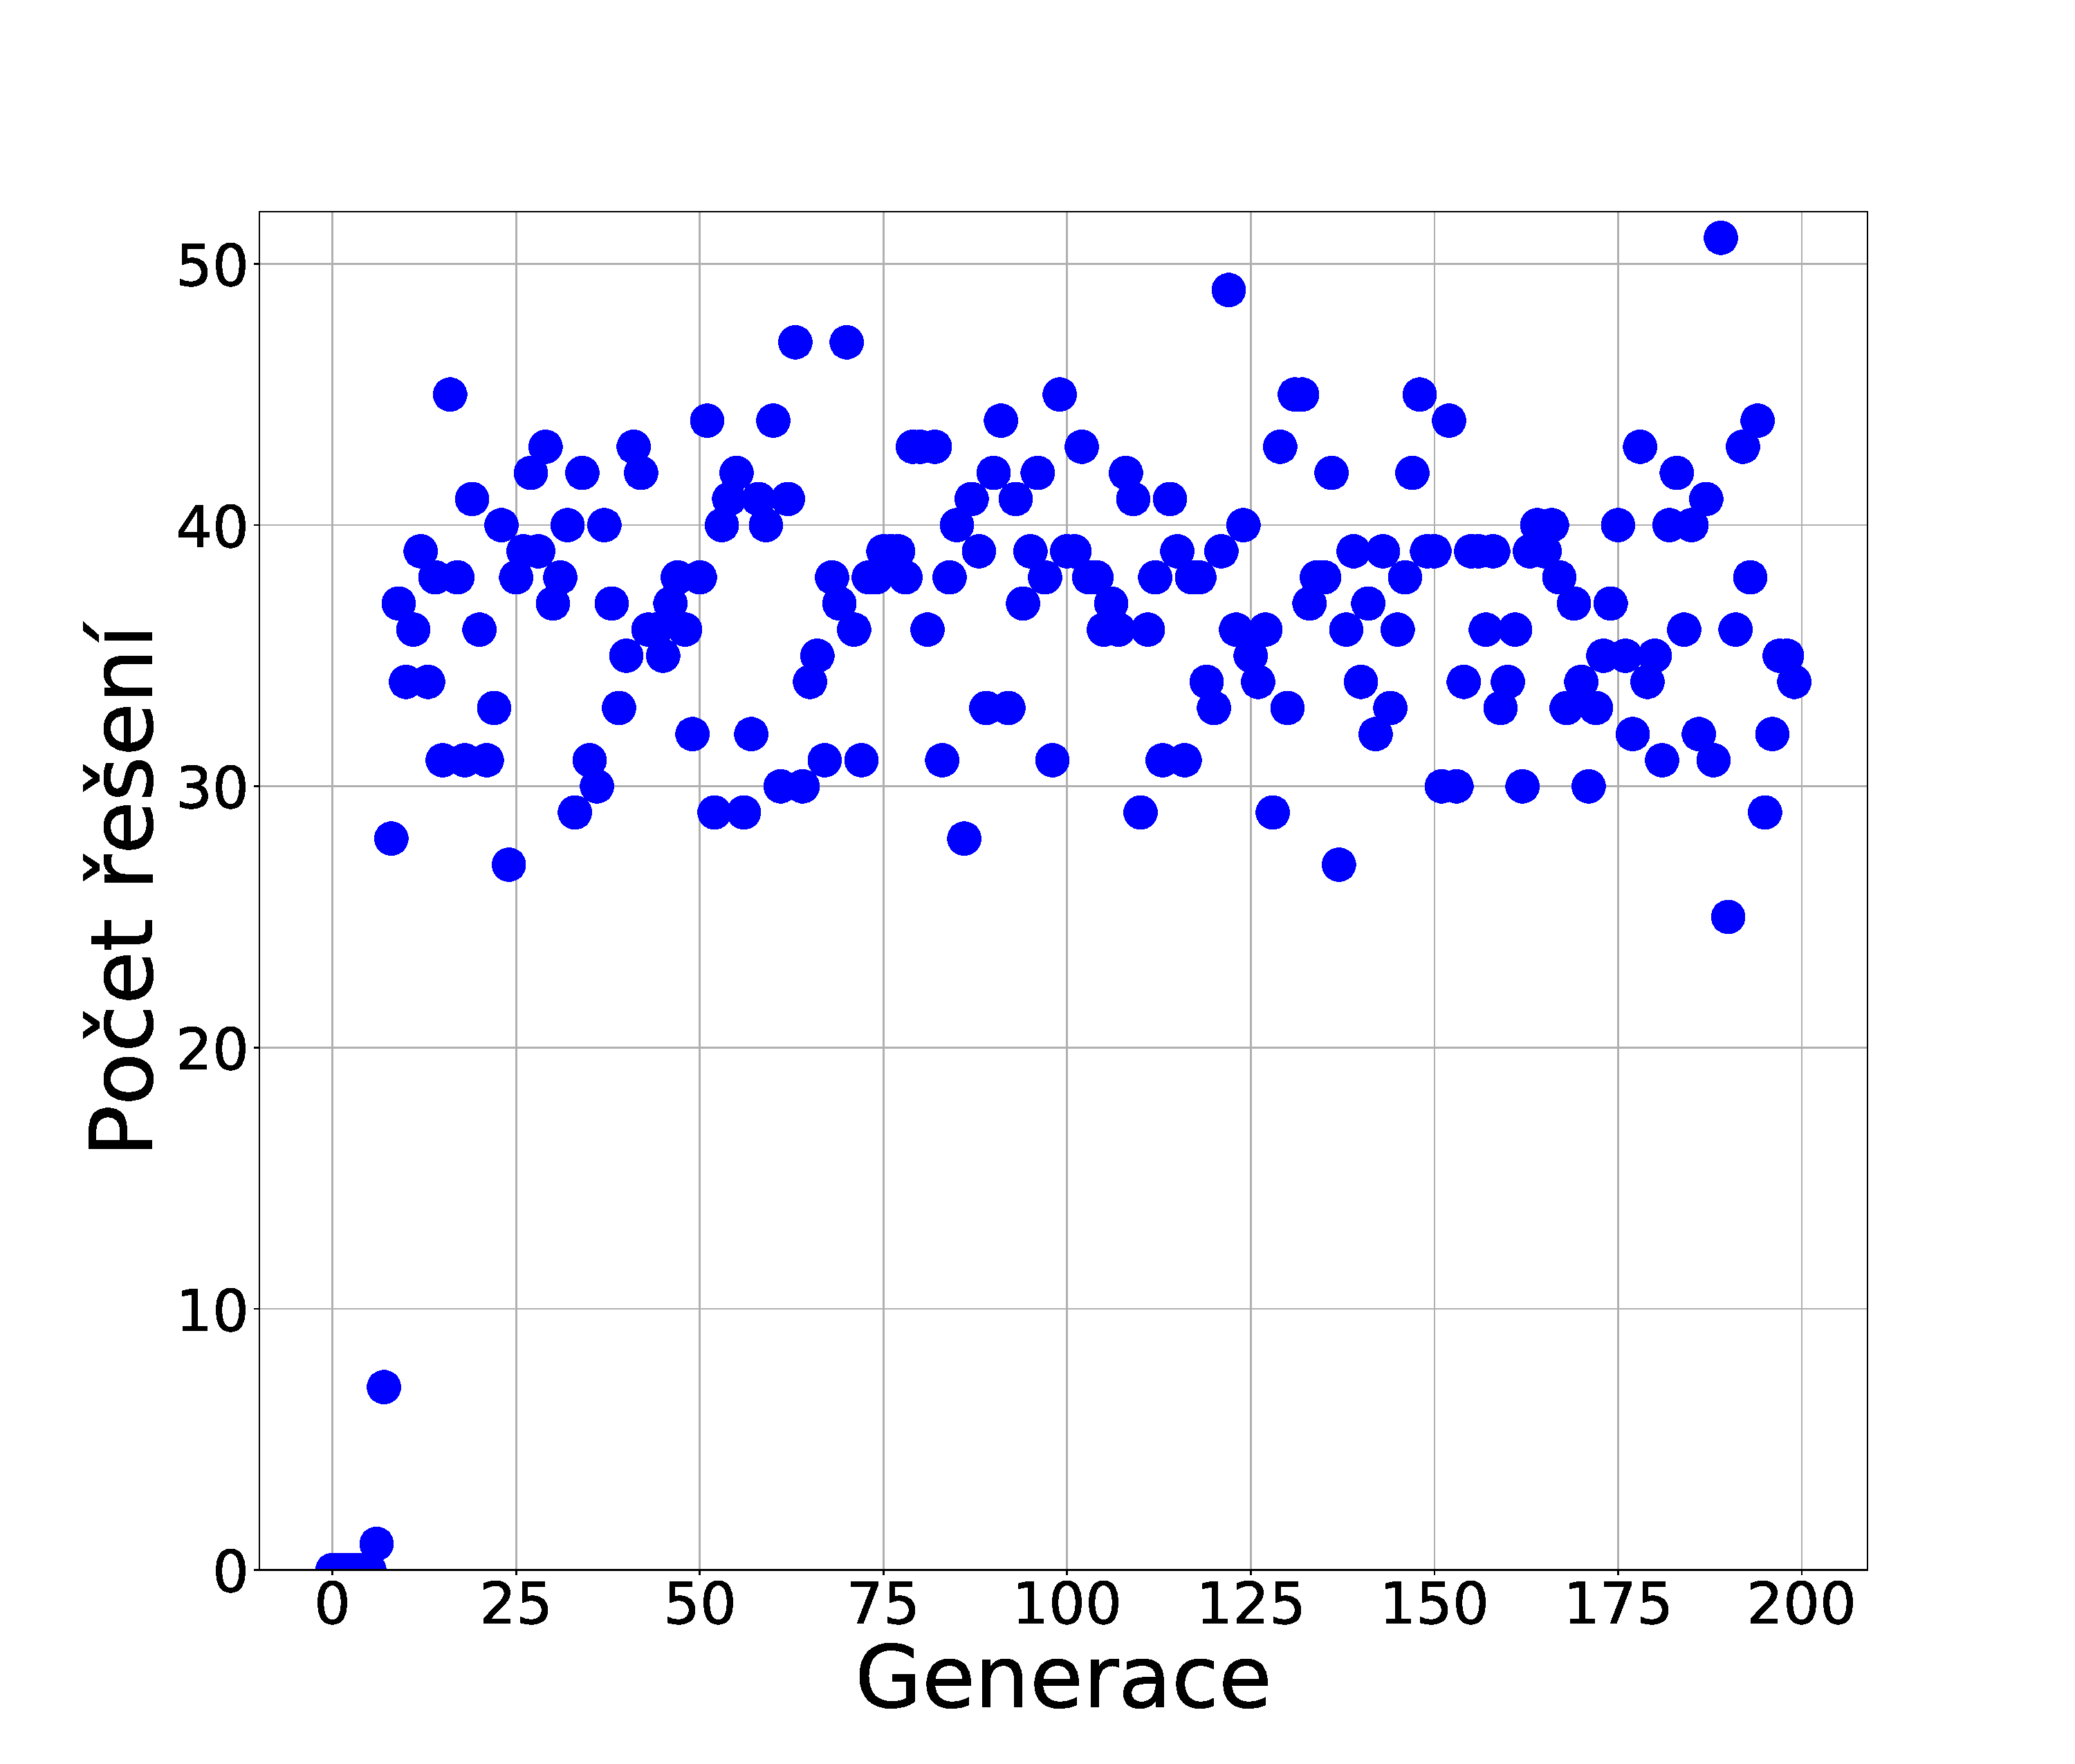
\includegraphics[width=\textwidth]{img/m051s.pdf} 
    \end{minipage}
    \\
    \begin{minipage}[c]{0.35\textwidth}
        \centering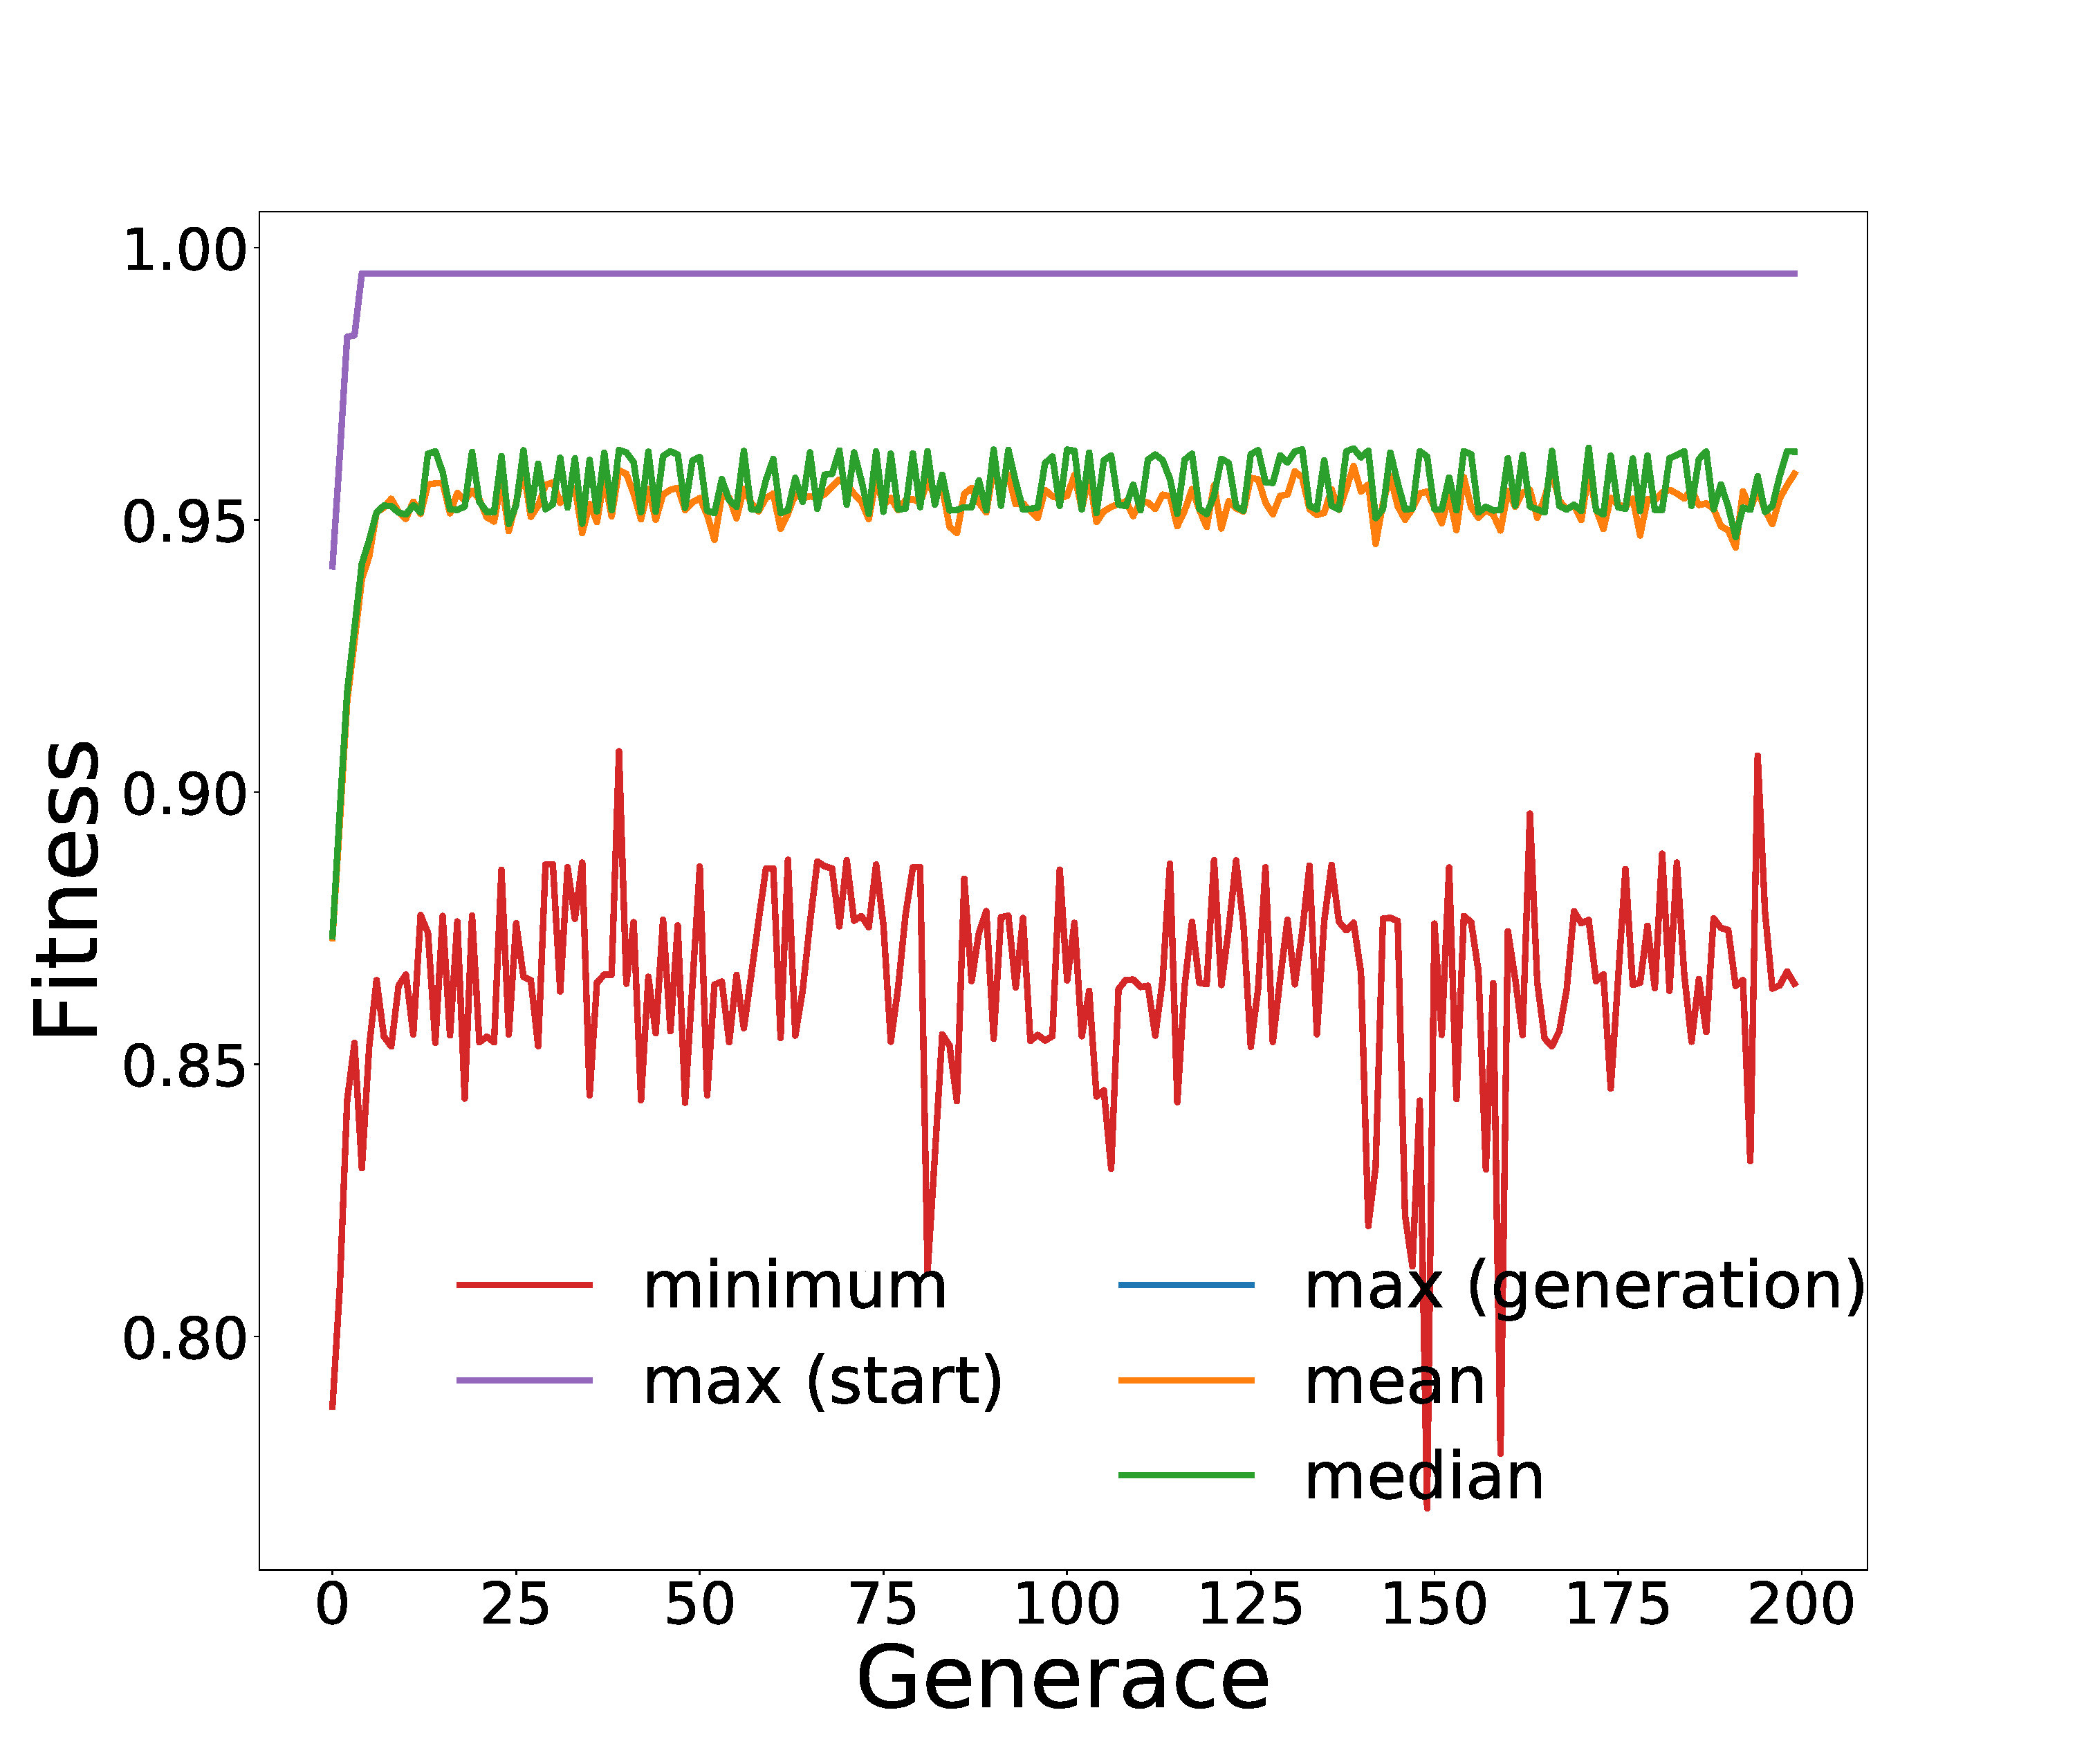
\includegraphics[width=\textwidth]{img/m101g.pdf} 
    \end{minipage}
    \begin{minipage}[c]{0.35\textwidth}
        \centering 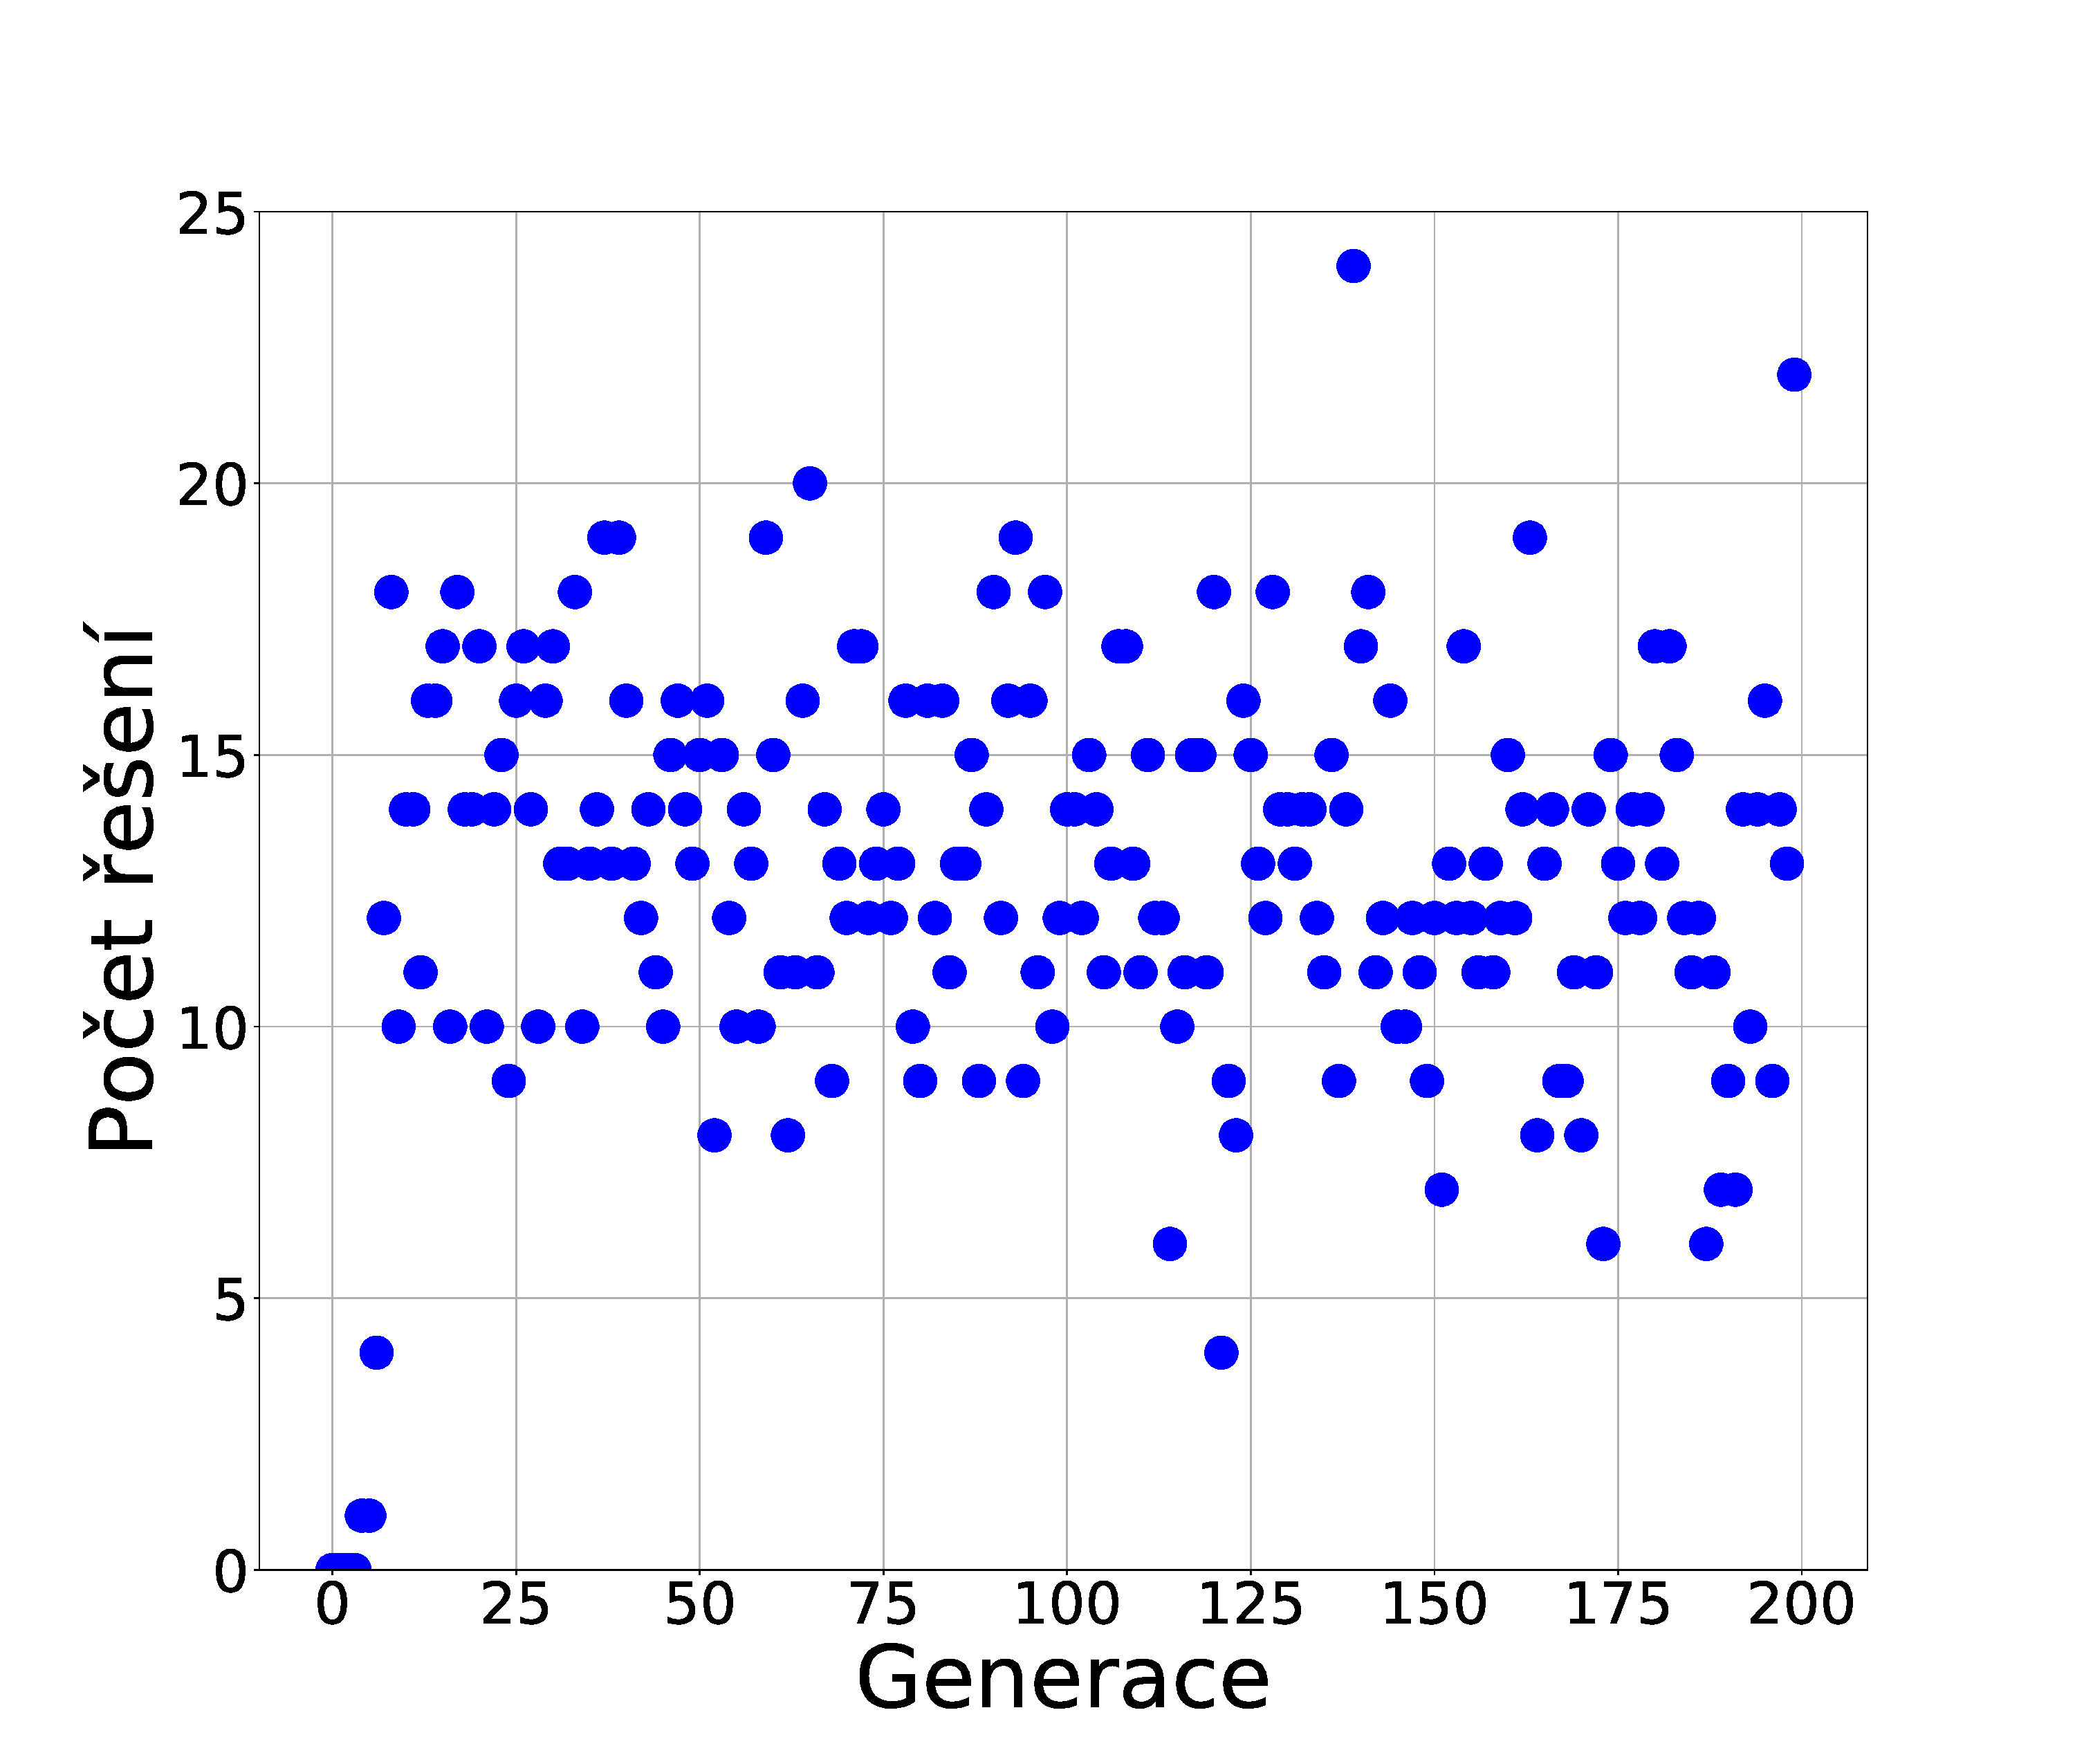
\includegraphics[width=\textwidth]{img/m101s.pdf} 
    \end{minipage}
    \begin{minipage}[c]{0.35\textwidth}
        \centering 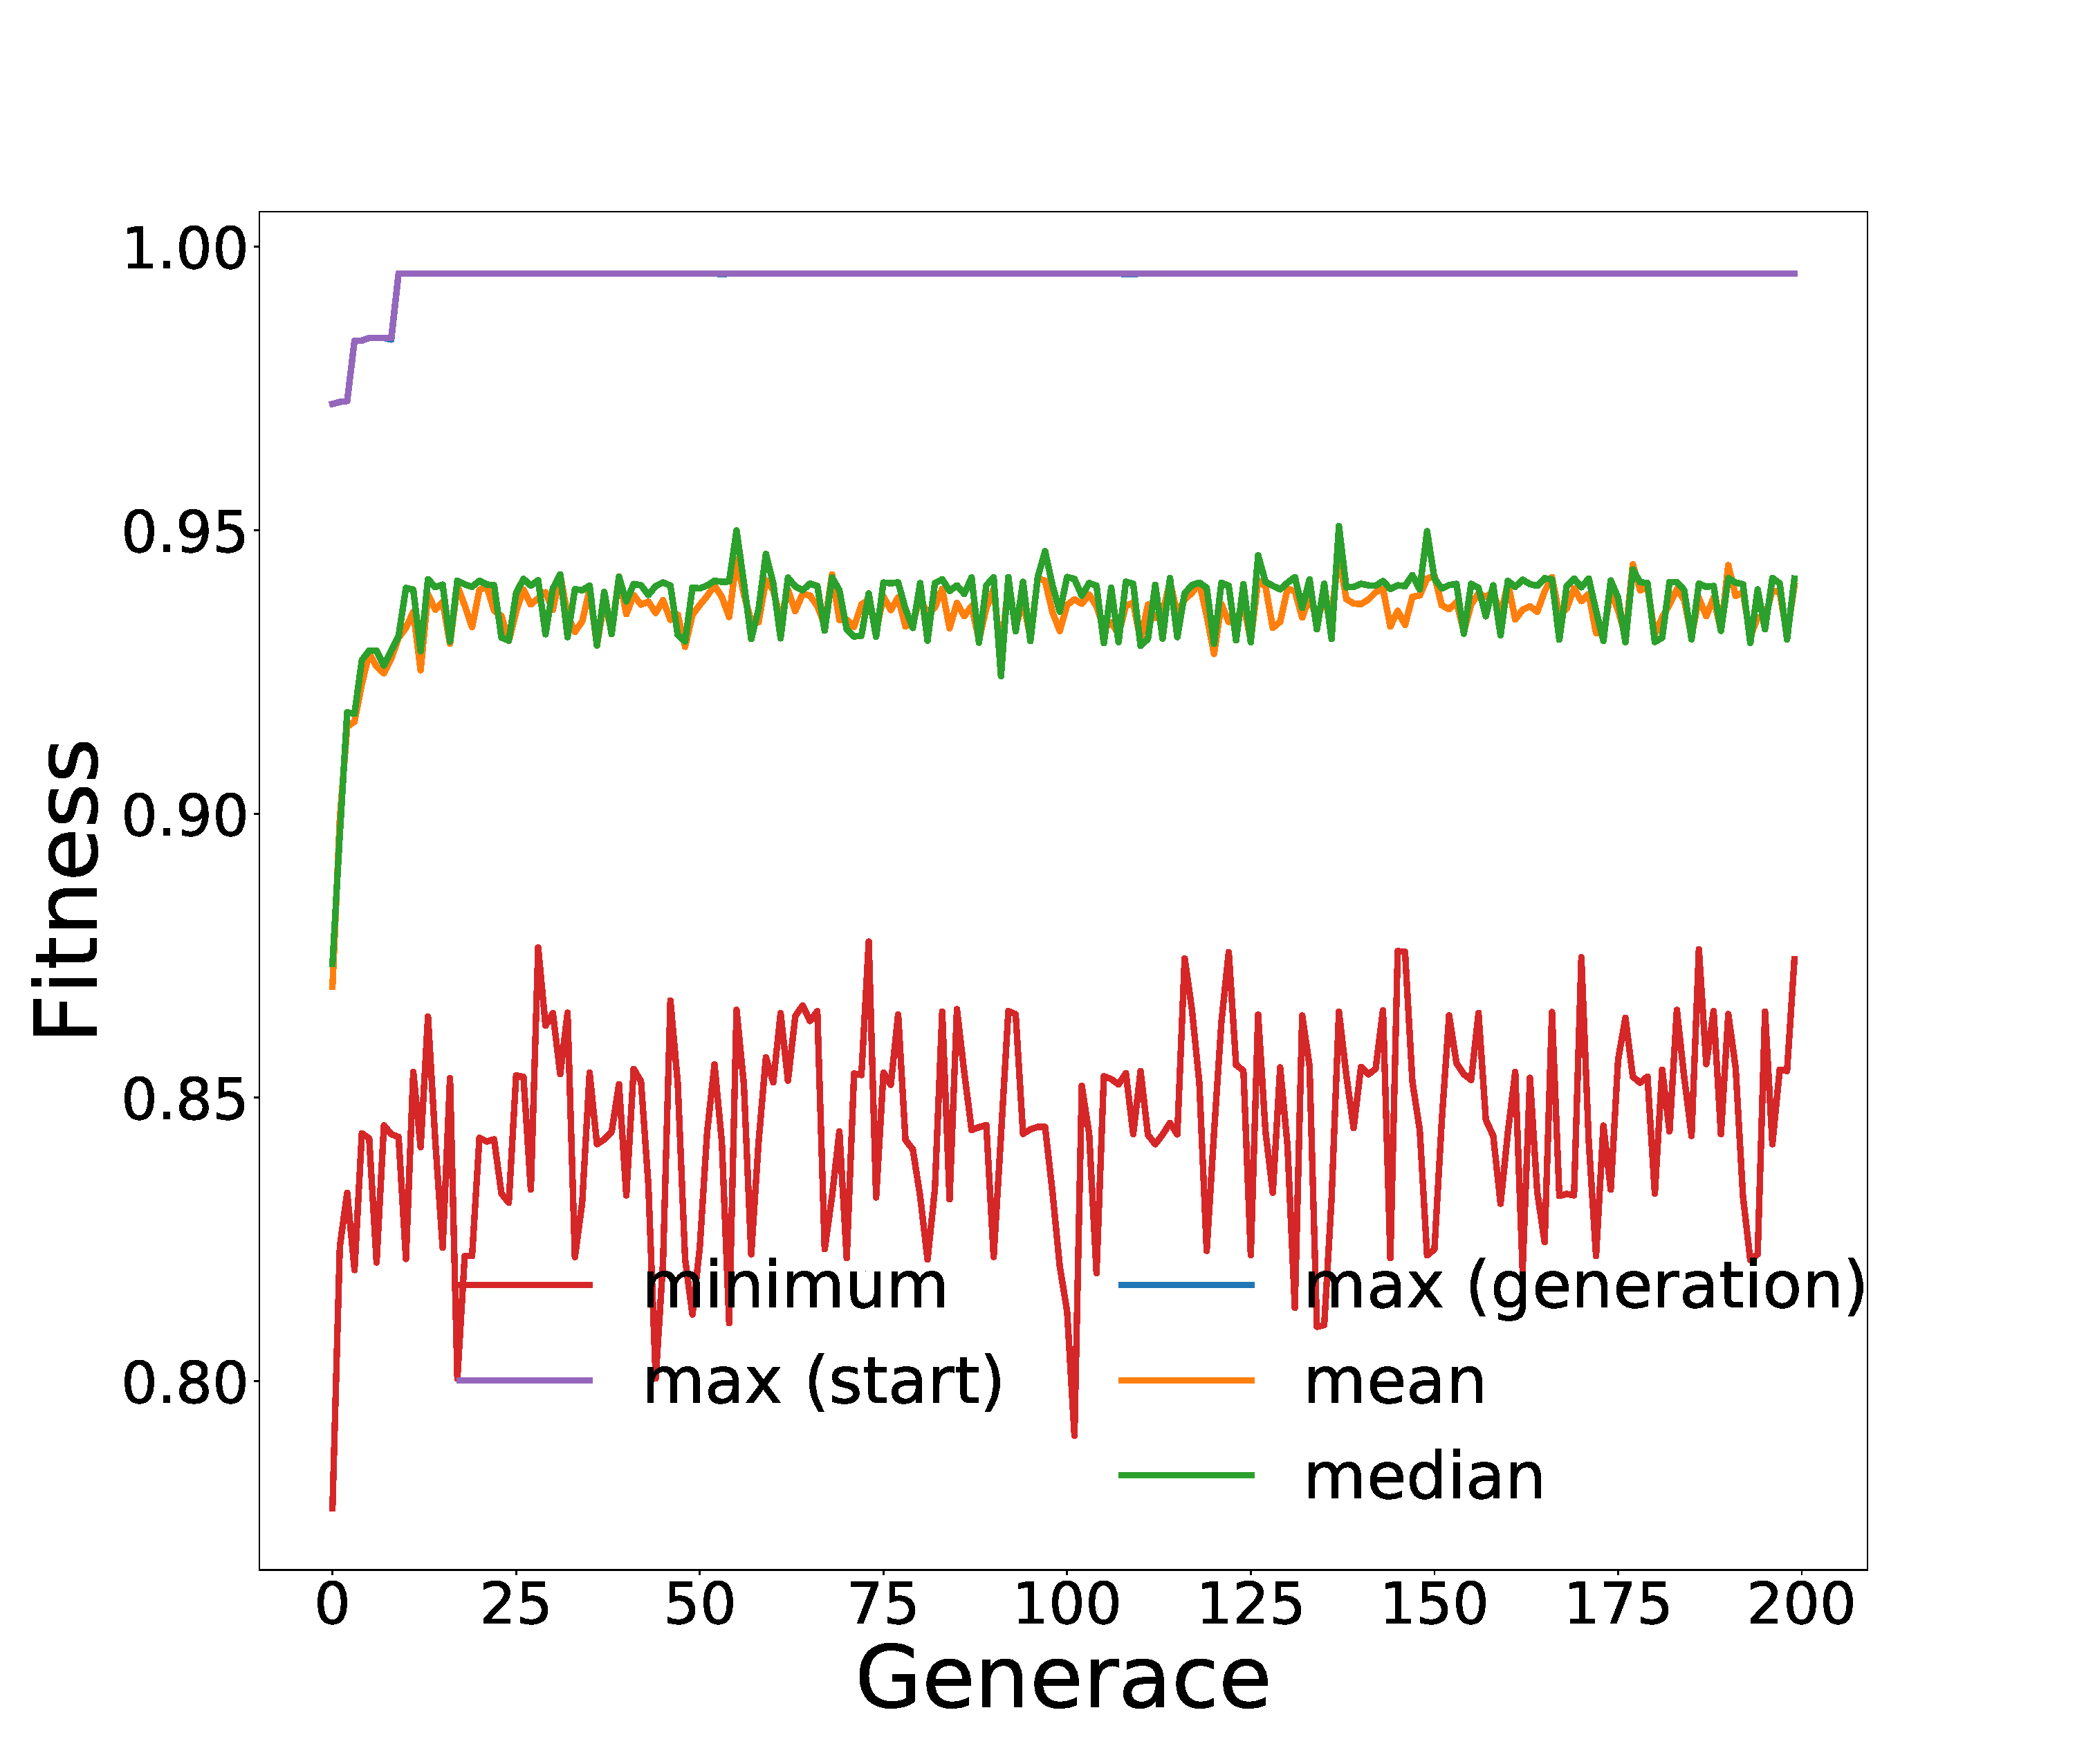
\includegraphics[width=\textwidth]{img/m151g.pdf} 
    \end{minipage}
    \begin{minipage}[c]{0.35\textwidth}
        \centering 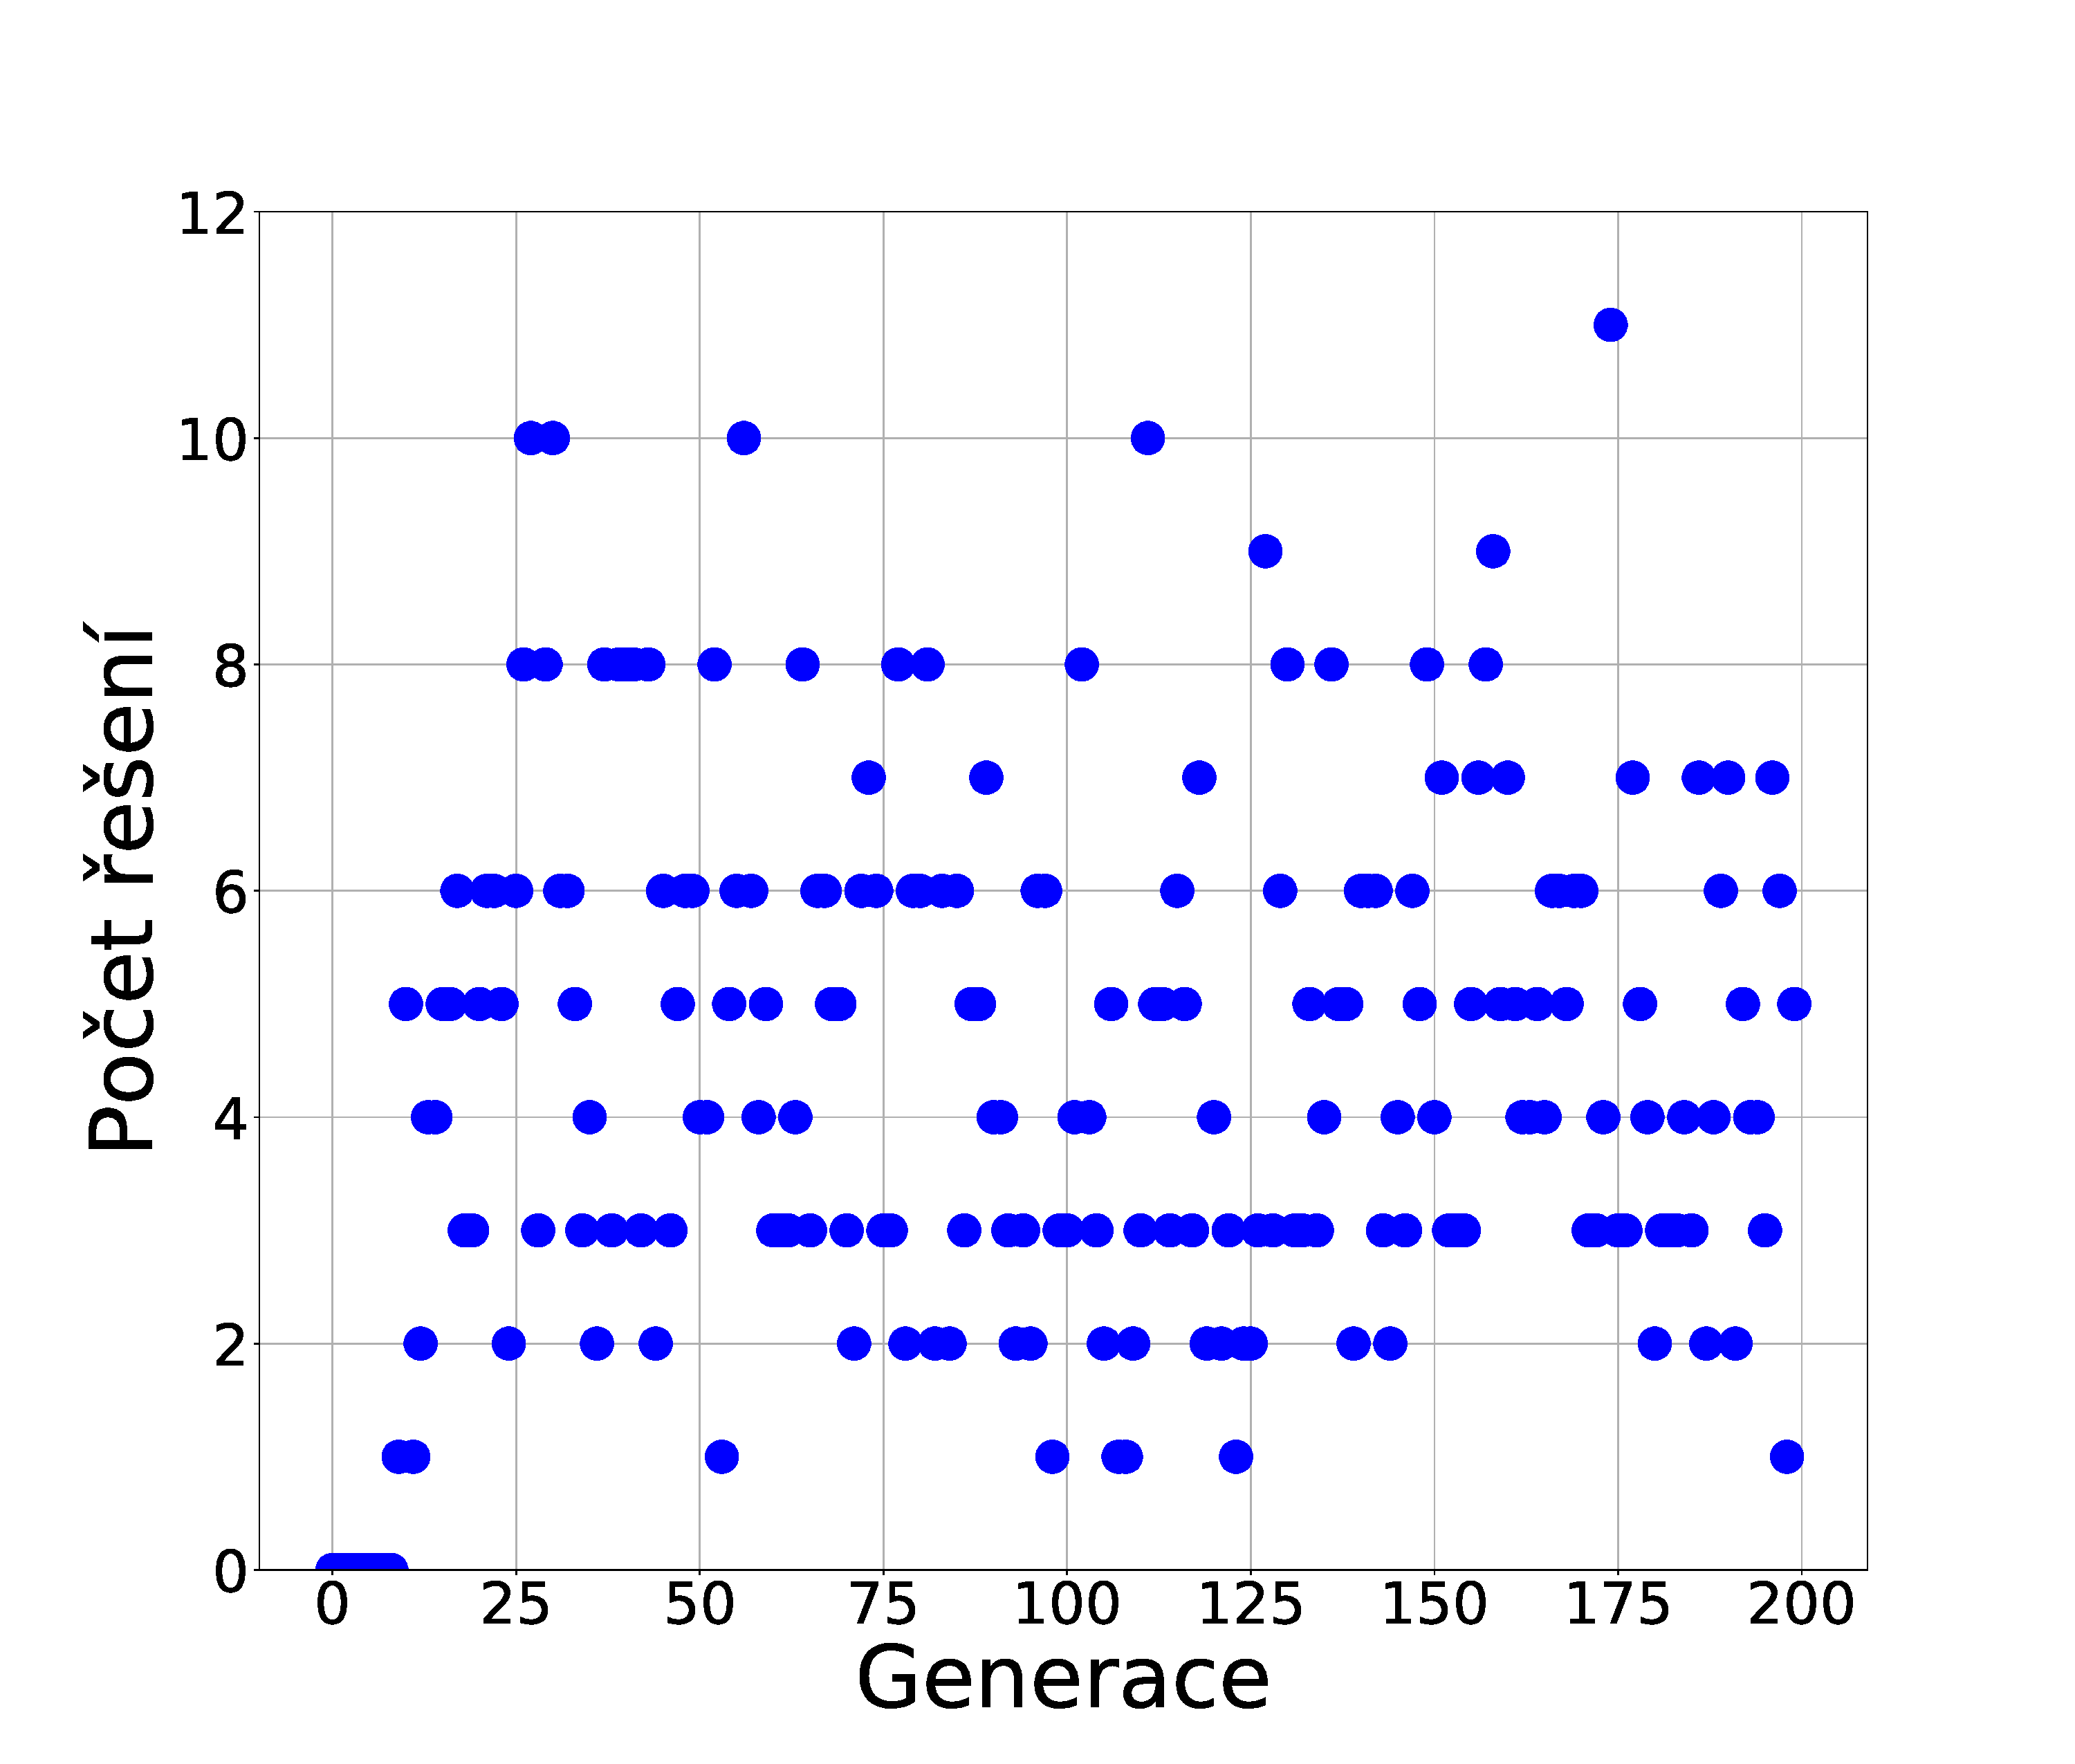
\includegraphics[width=\textwidth]{img/m151s.pdf} 
    \end{minipage}
    \\
    \begin{minipage}[c]{0.35\textwidth}
        \centering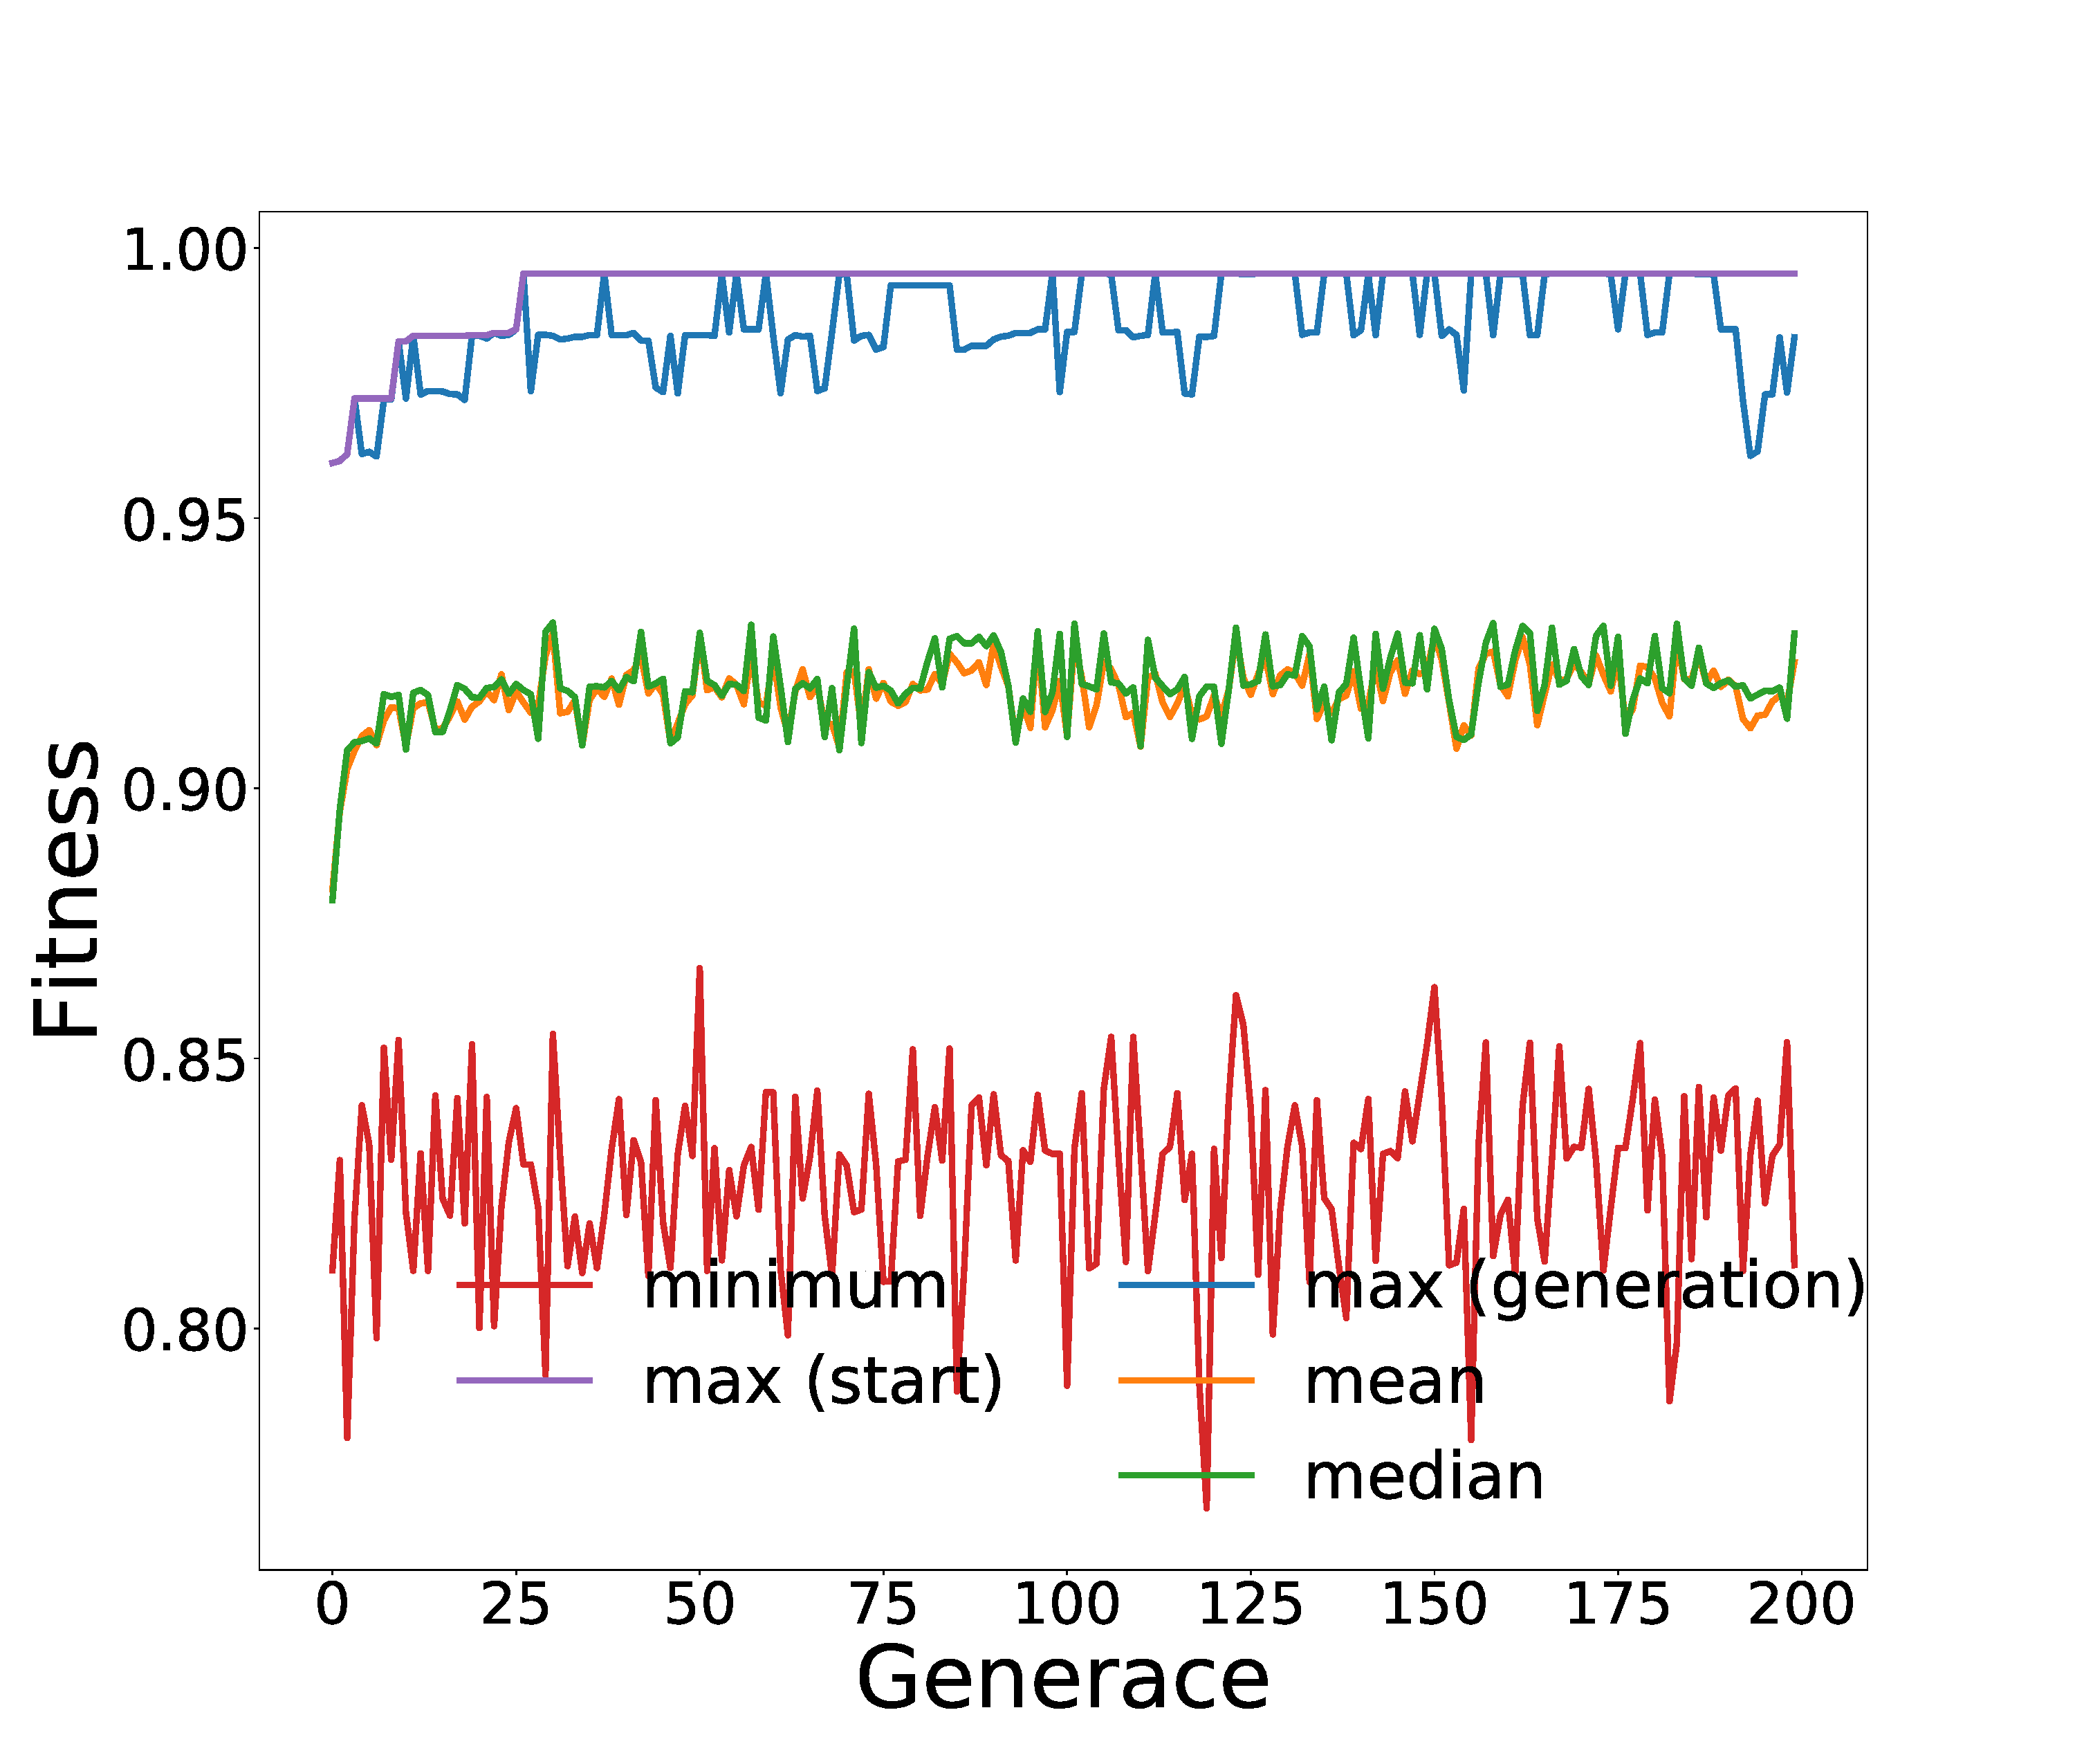
\includegraphics[width=\textwidth]{img/m201g.pdf} 
    \end{minipage}
    \begin{minipage}[c]{0.35\textwidth}
        \centering 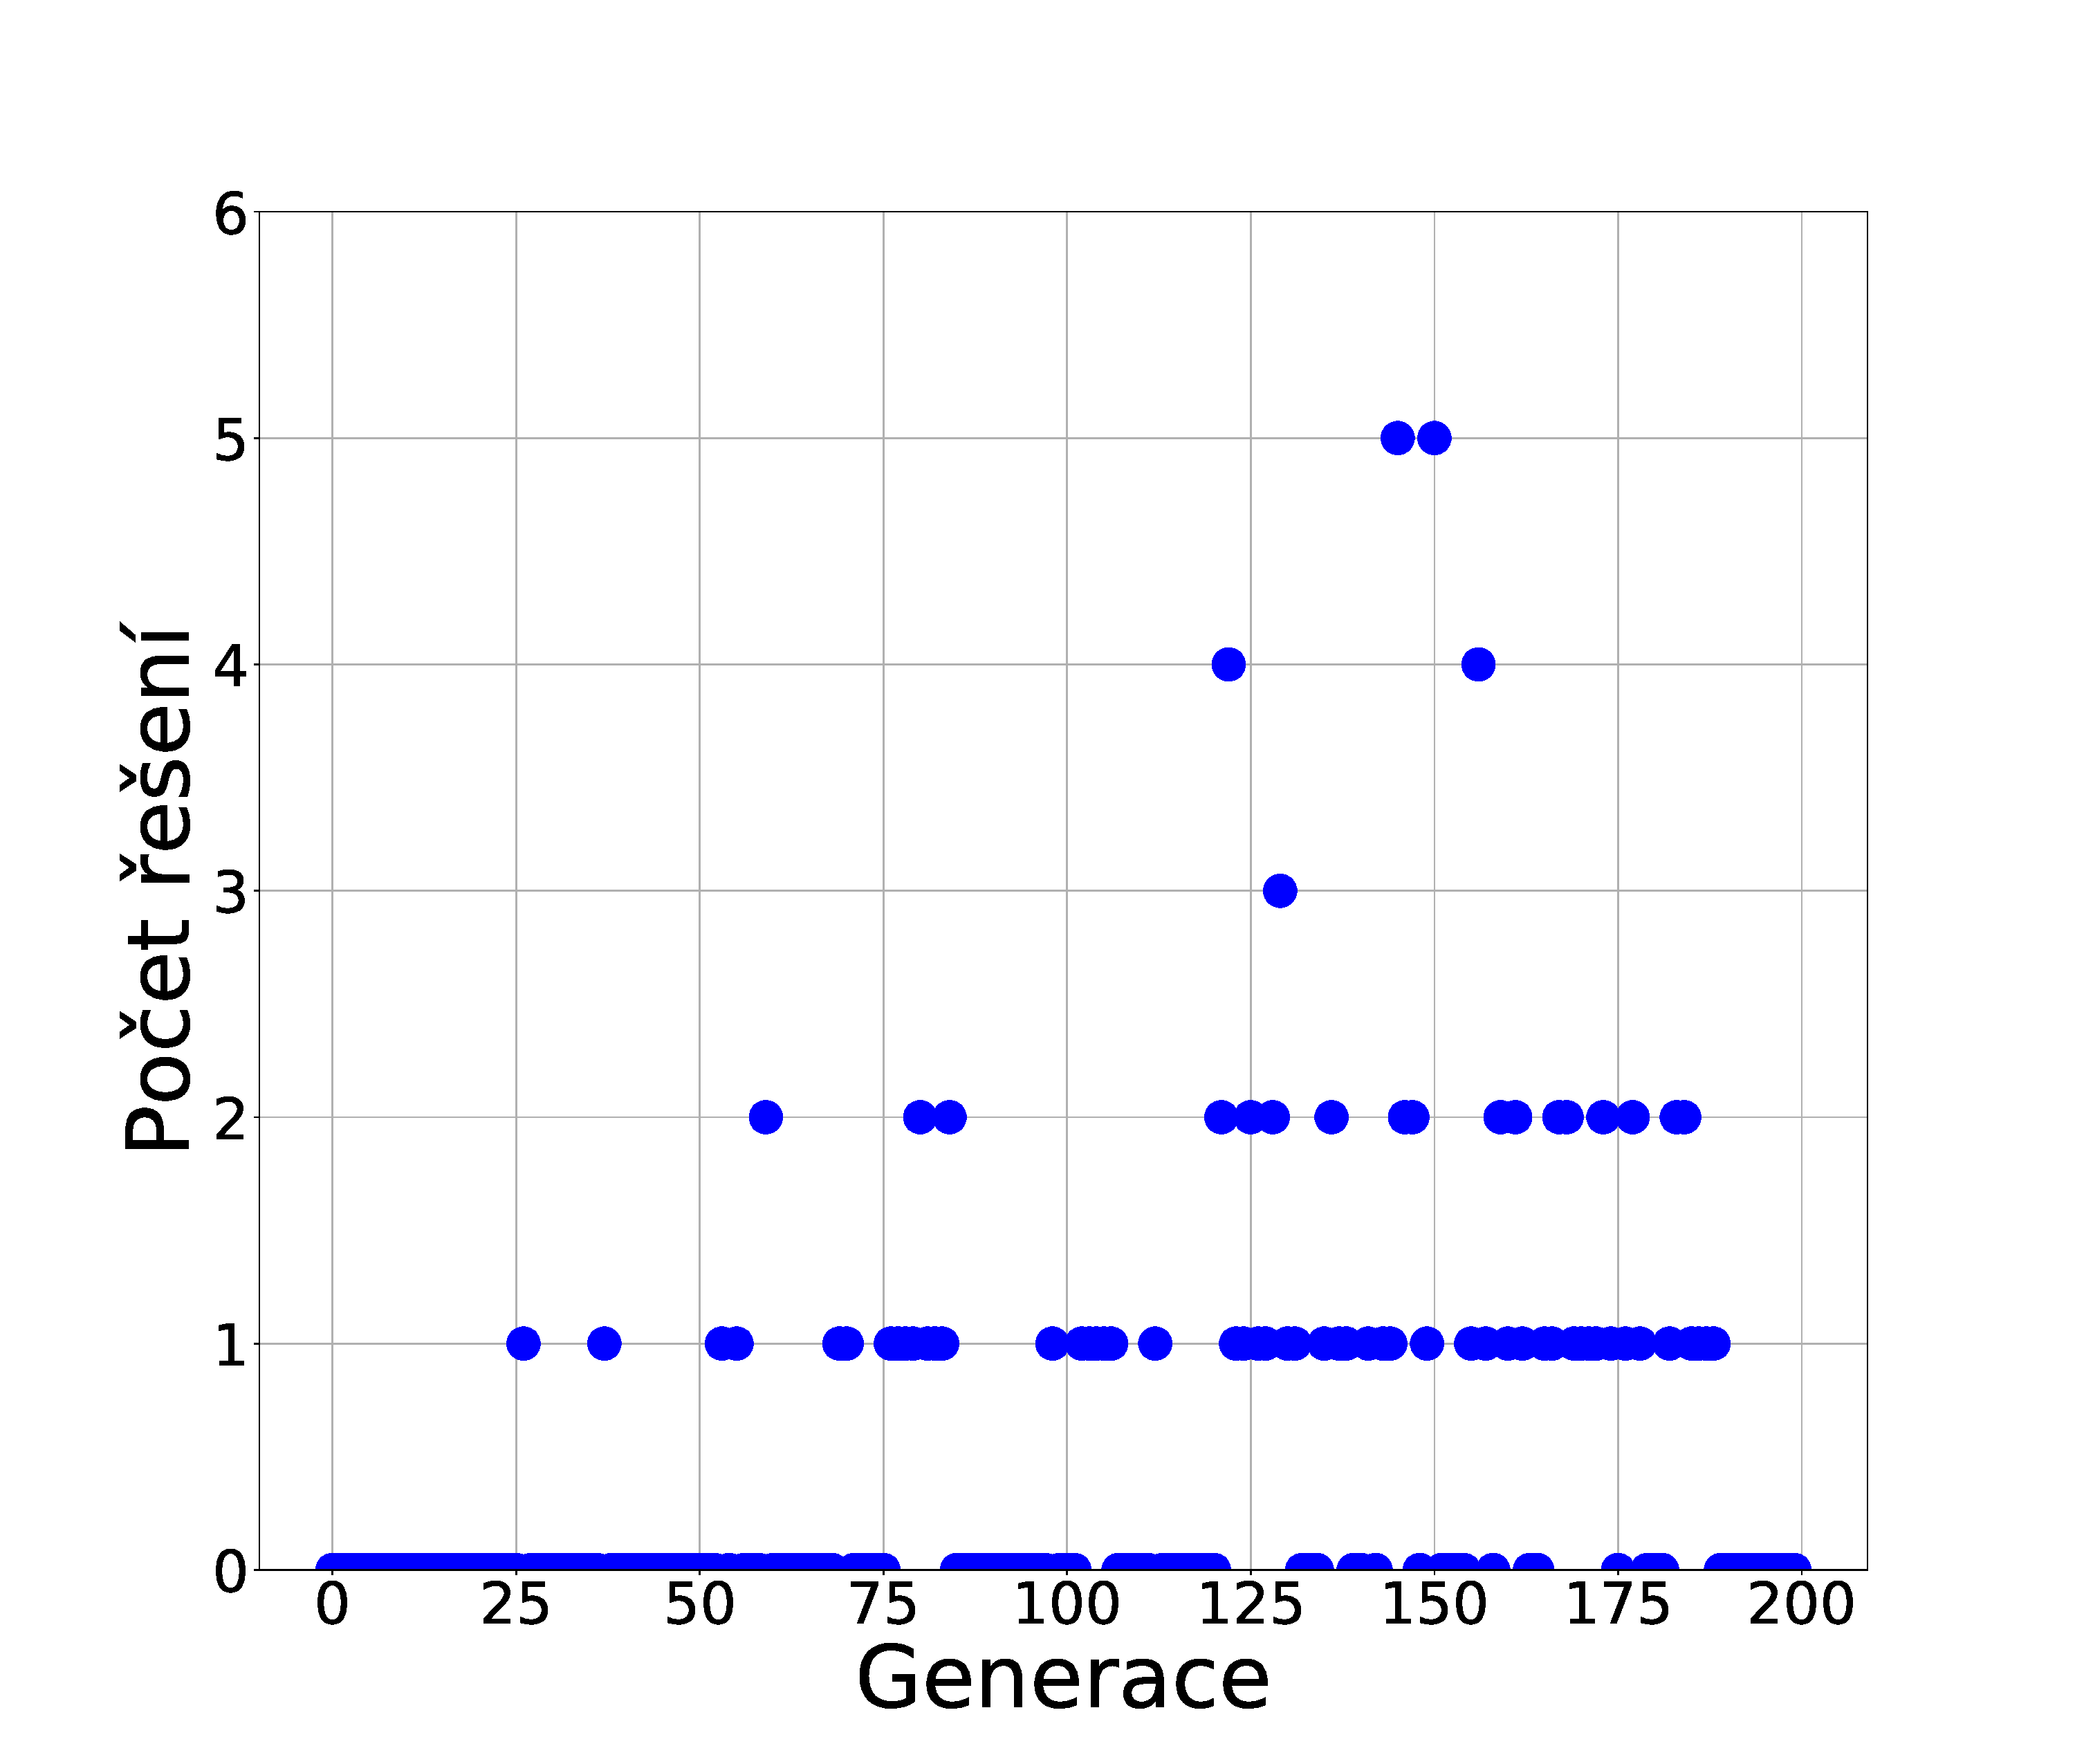
\includegraphics[width=\textwidth]{img/m201s.pdf} 
    \end{minipage}
    \begin{minipage}[c]{0.35\textwidth}
        \centering 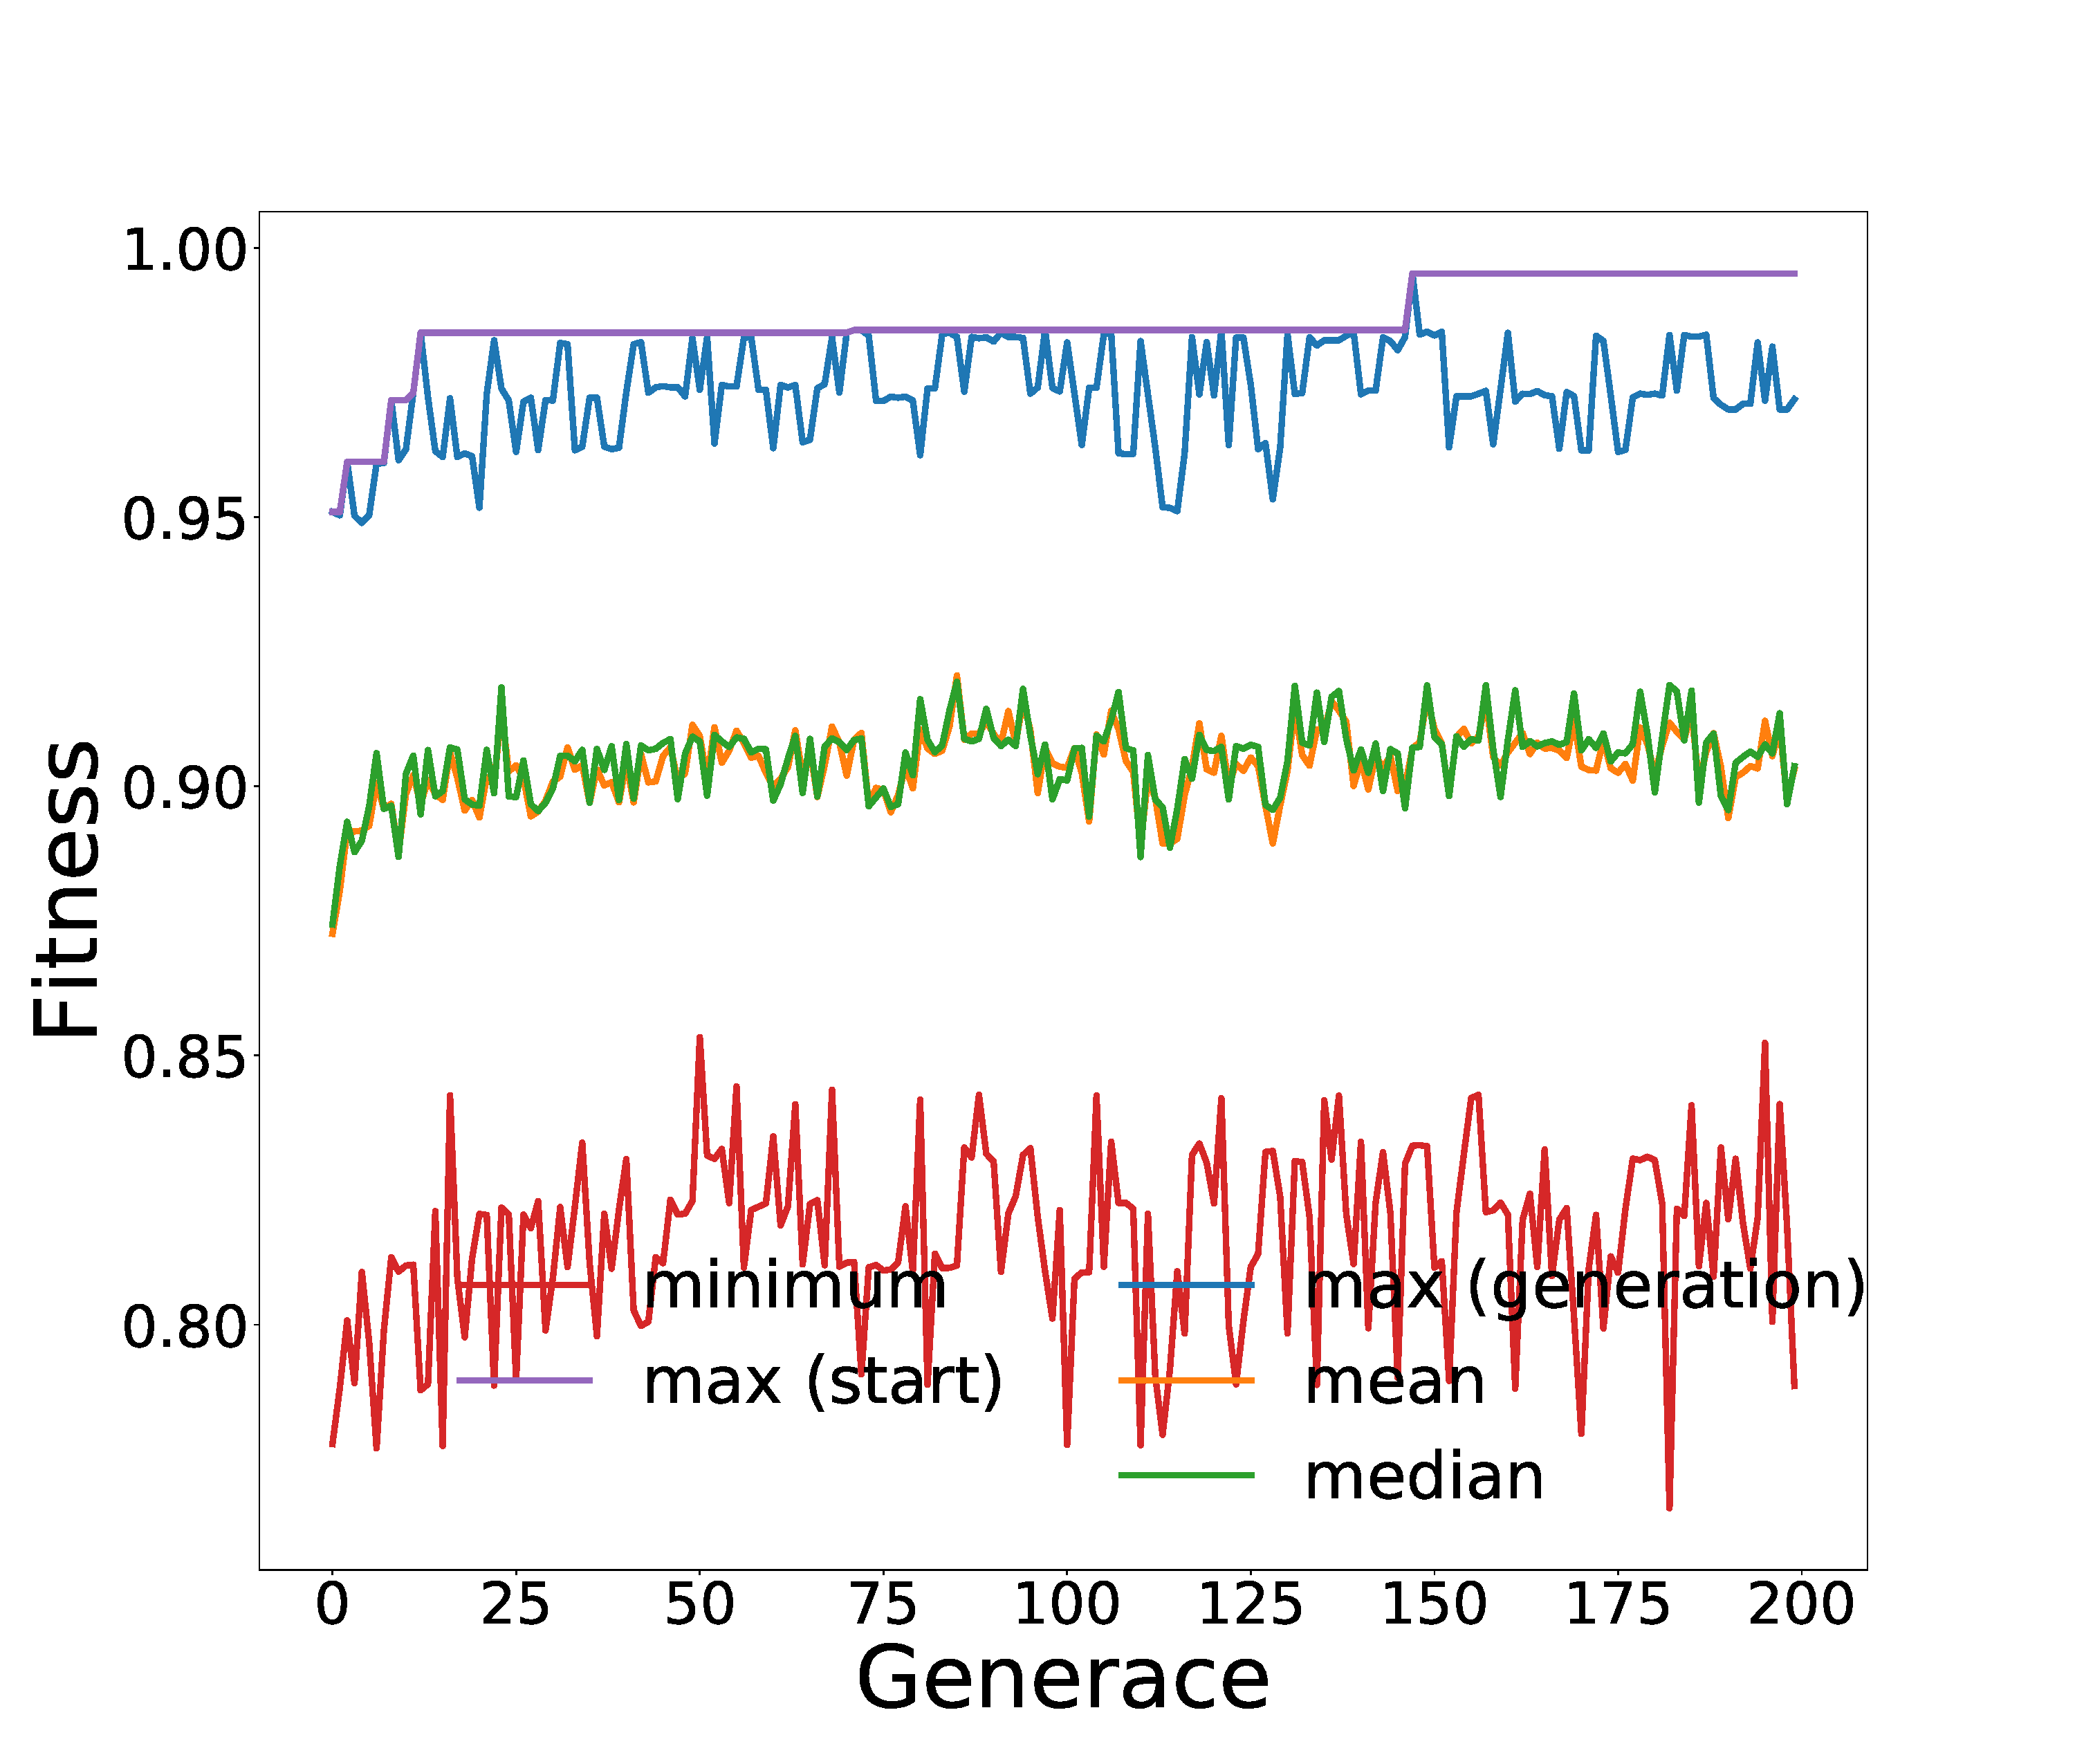
\includegraphics[width=\textwidth]{img/m251g.pdf} 
    \end{minipage}
    \begin{minipage}[c]{0.35\textwidth}
        \centering 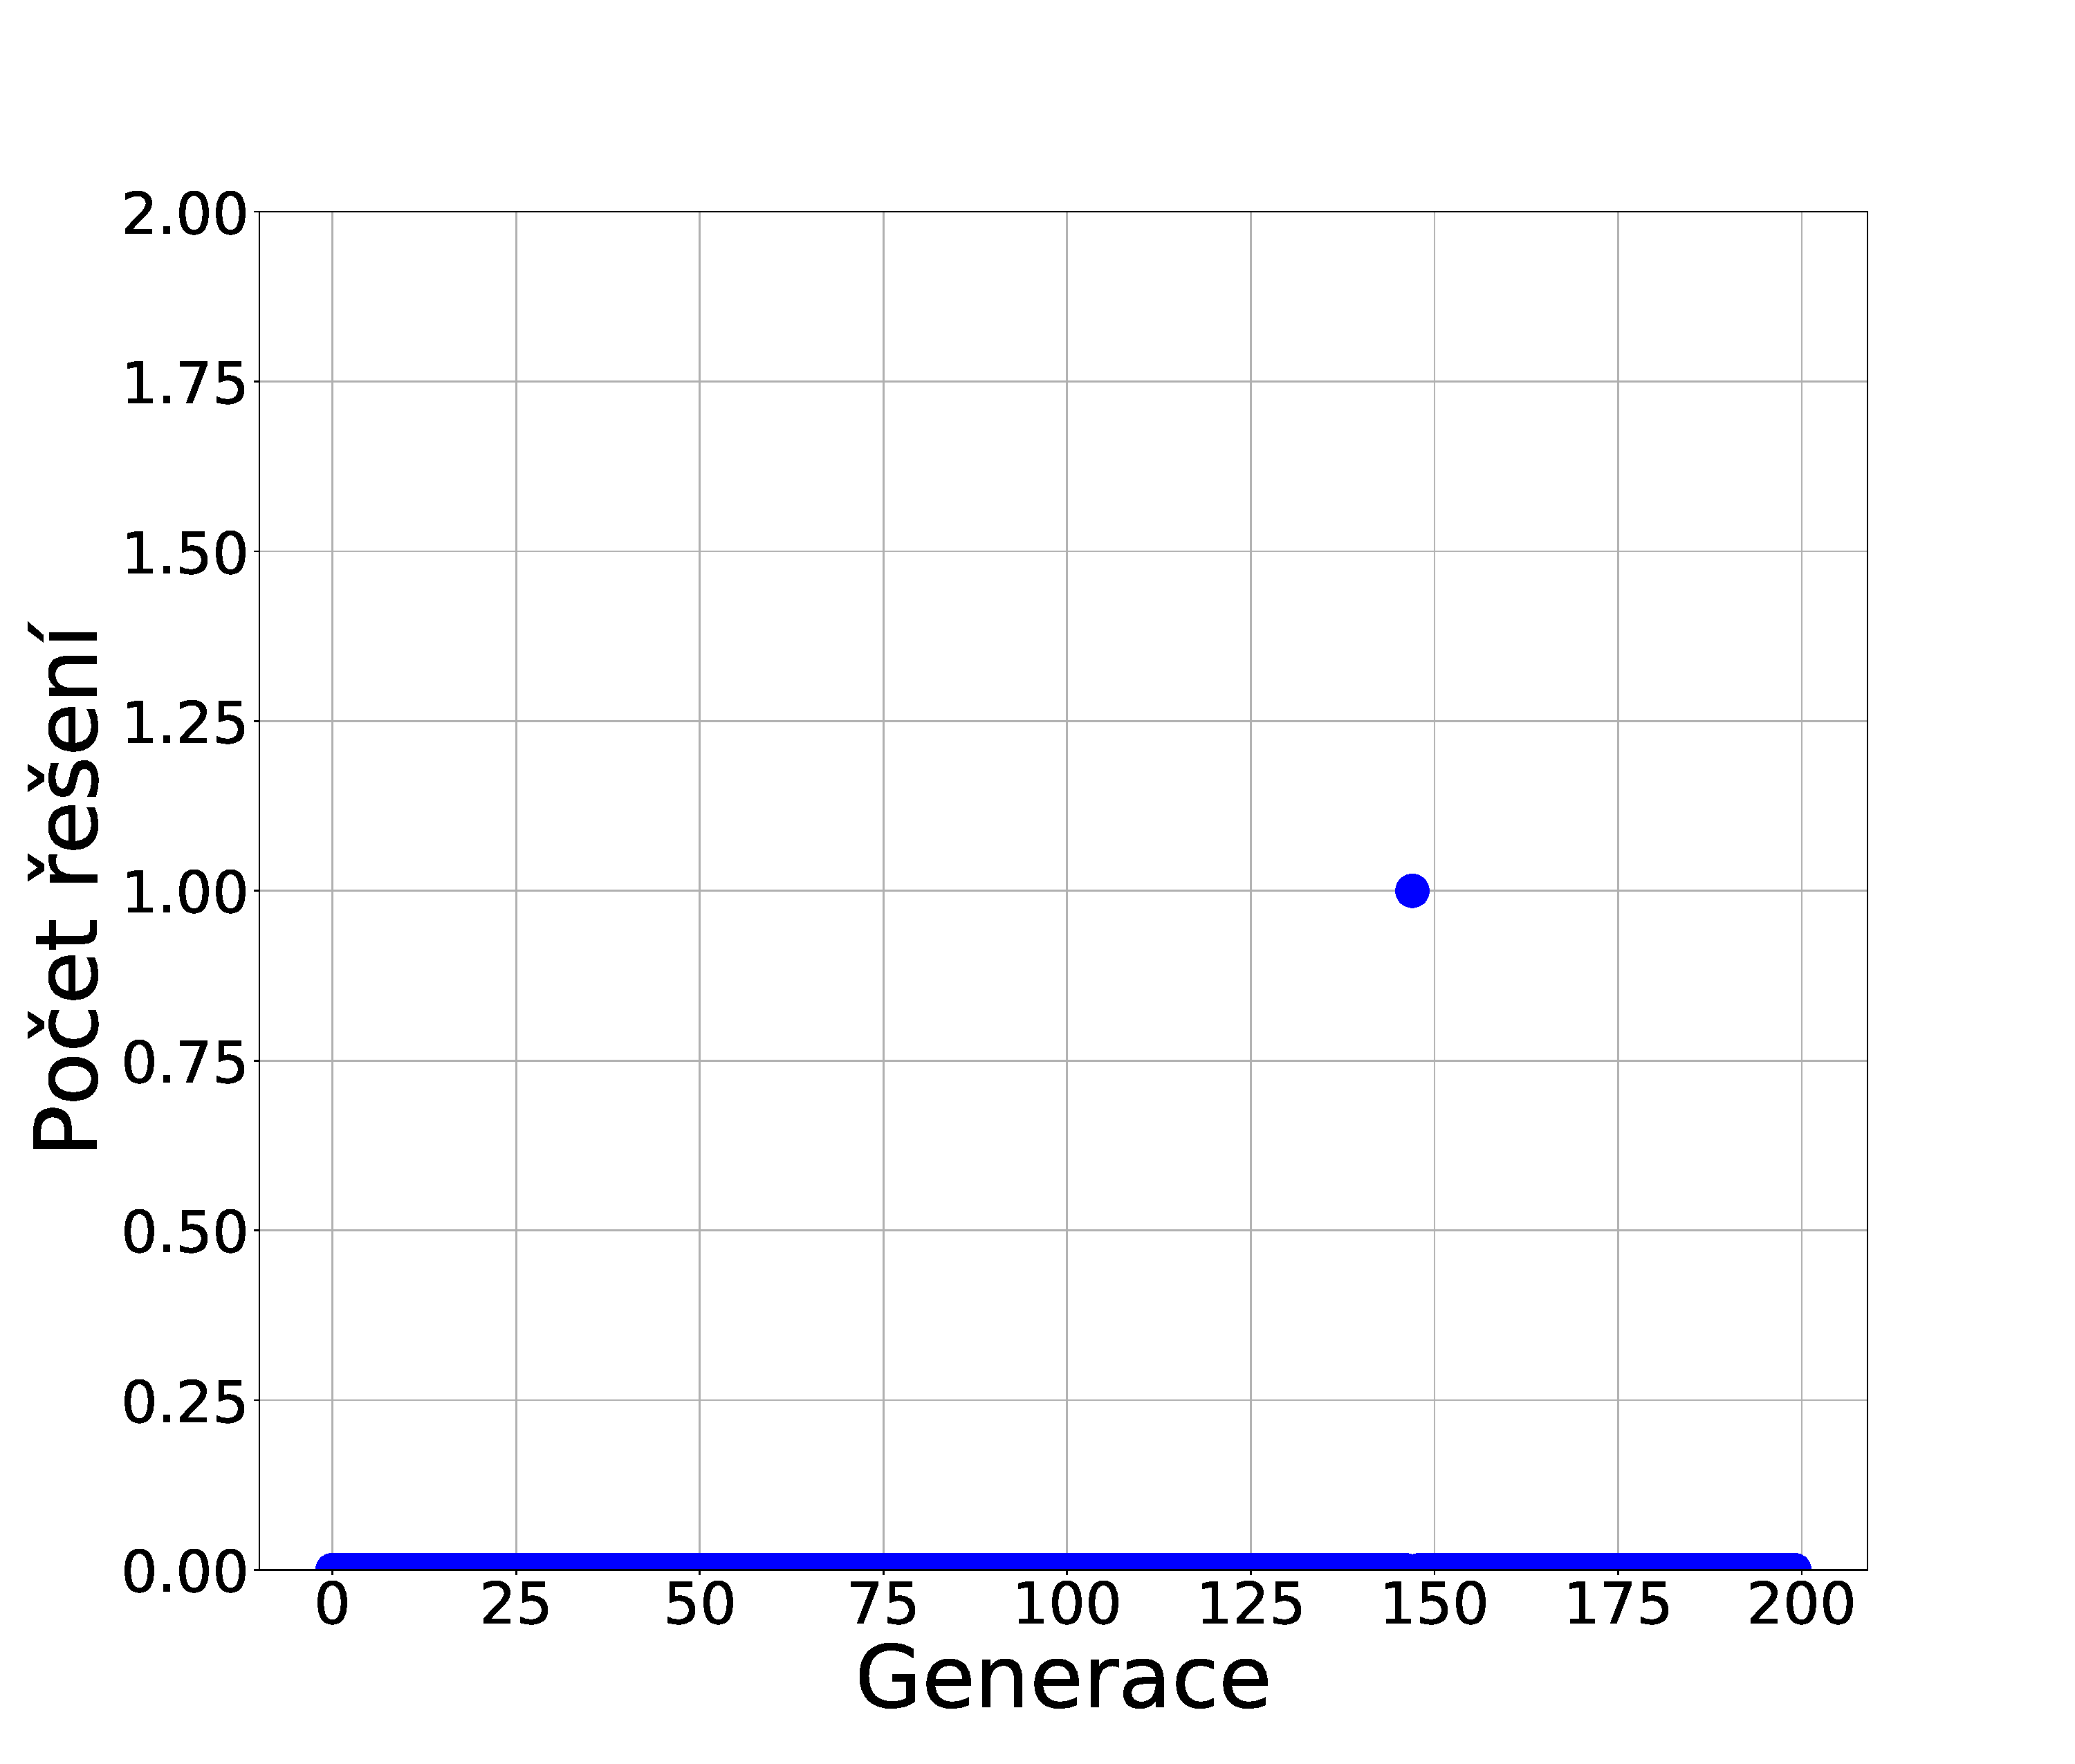
\includegraphics[width=\textwidth]{img/m251s.pdf} 
    \end{minipage}
   \caption{Na grafech je zachycen vliv mutace na genetický algoritmus a na výsledná řešení v populaci. Grafy jsou po dvojicích zleva do prava a ze zhora dolů pro hodnoty mutace od 0,001 po 0,251 včetně s krokem 0,05.}\label{fig:mutAll}
\end{figure} 
\end{landscape} 

Na další obrázku \ref{fig:mutAll} jsem se pokusil zachytit, jak hodnota mutace působí na průběh řešení a~jaký má vliv na skladbu populace. Na prvních grafech s velmi malou hodnotou mutace je patrná omezená skladba populace, kde po pár generacích jsou všichni jedinci v nějakém stejném optimu, které nemusí být globální a prozkoumávaný prostor je velice malý. Se zvětšující se mutací, také roste diverzita populace a již se zde nenachází tolik řešení a může být prozkoumáno větší okolí. V rostoucí mutací vídíme i ubývající počet řešení v populaci. Na posledních obrázcích je patrná populace, která již nesměřuje k řešení, ale mutace překonává selekční tlak a je to vlastně zkoumání náhodných konfigurací, ale i zde se v jedné generaci díky randomizovanosti a jednodušímu problému podařilo nalézt řešení. 

\begin{figure}
	\centering
    \begin{minipage}[c]{0.48\textwidth}
        \centering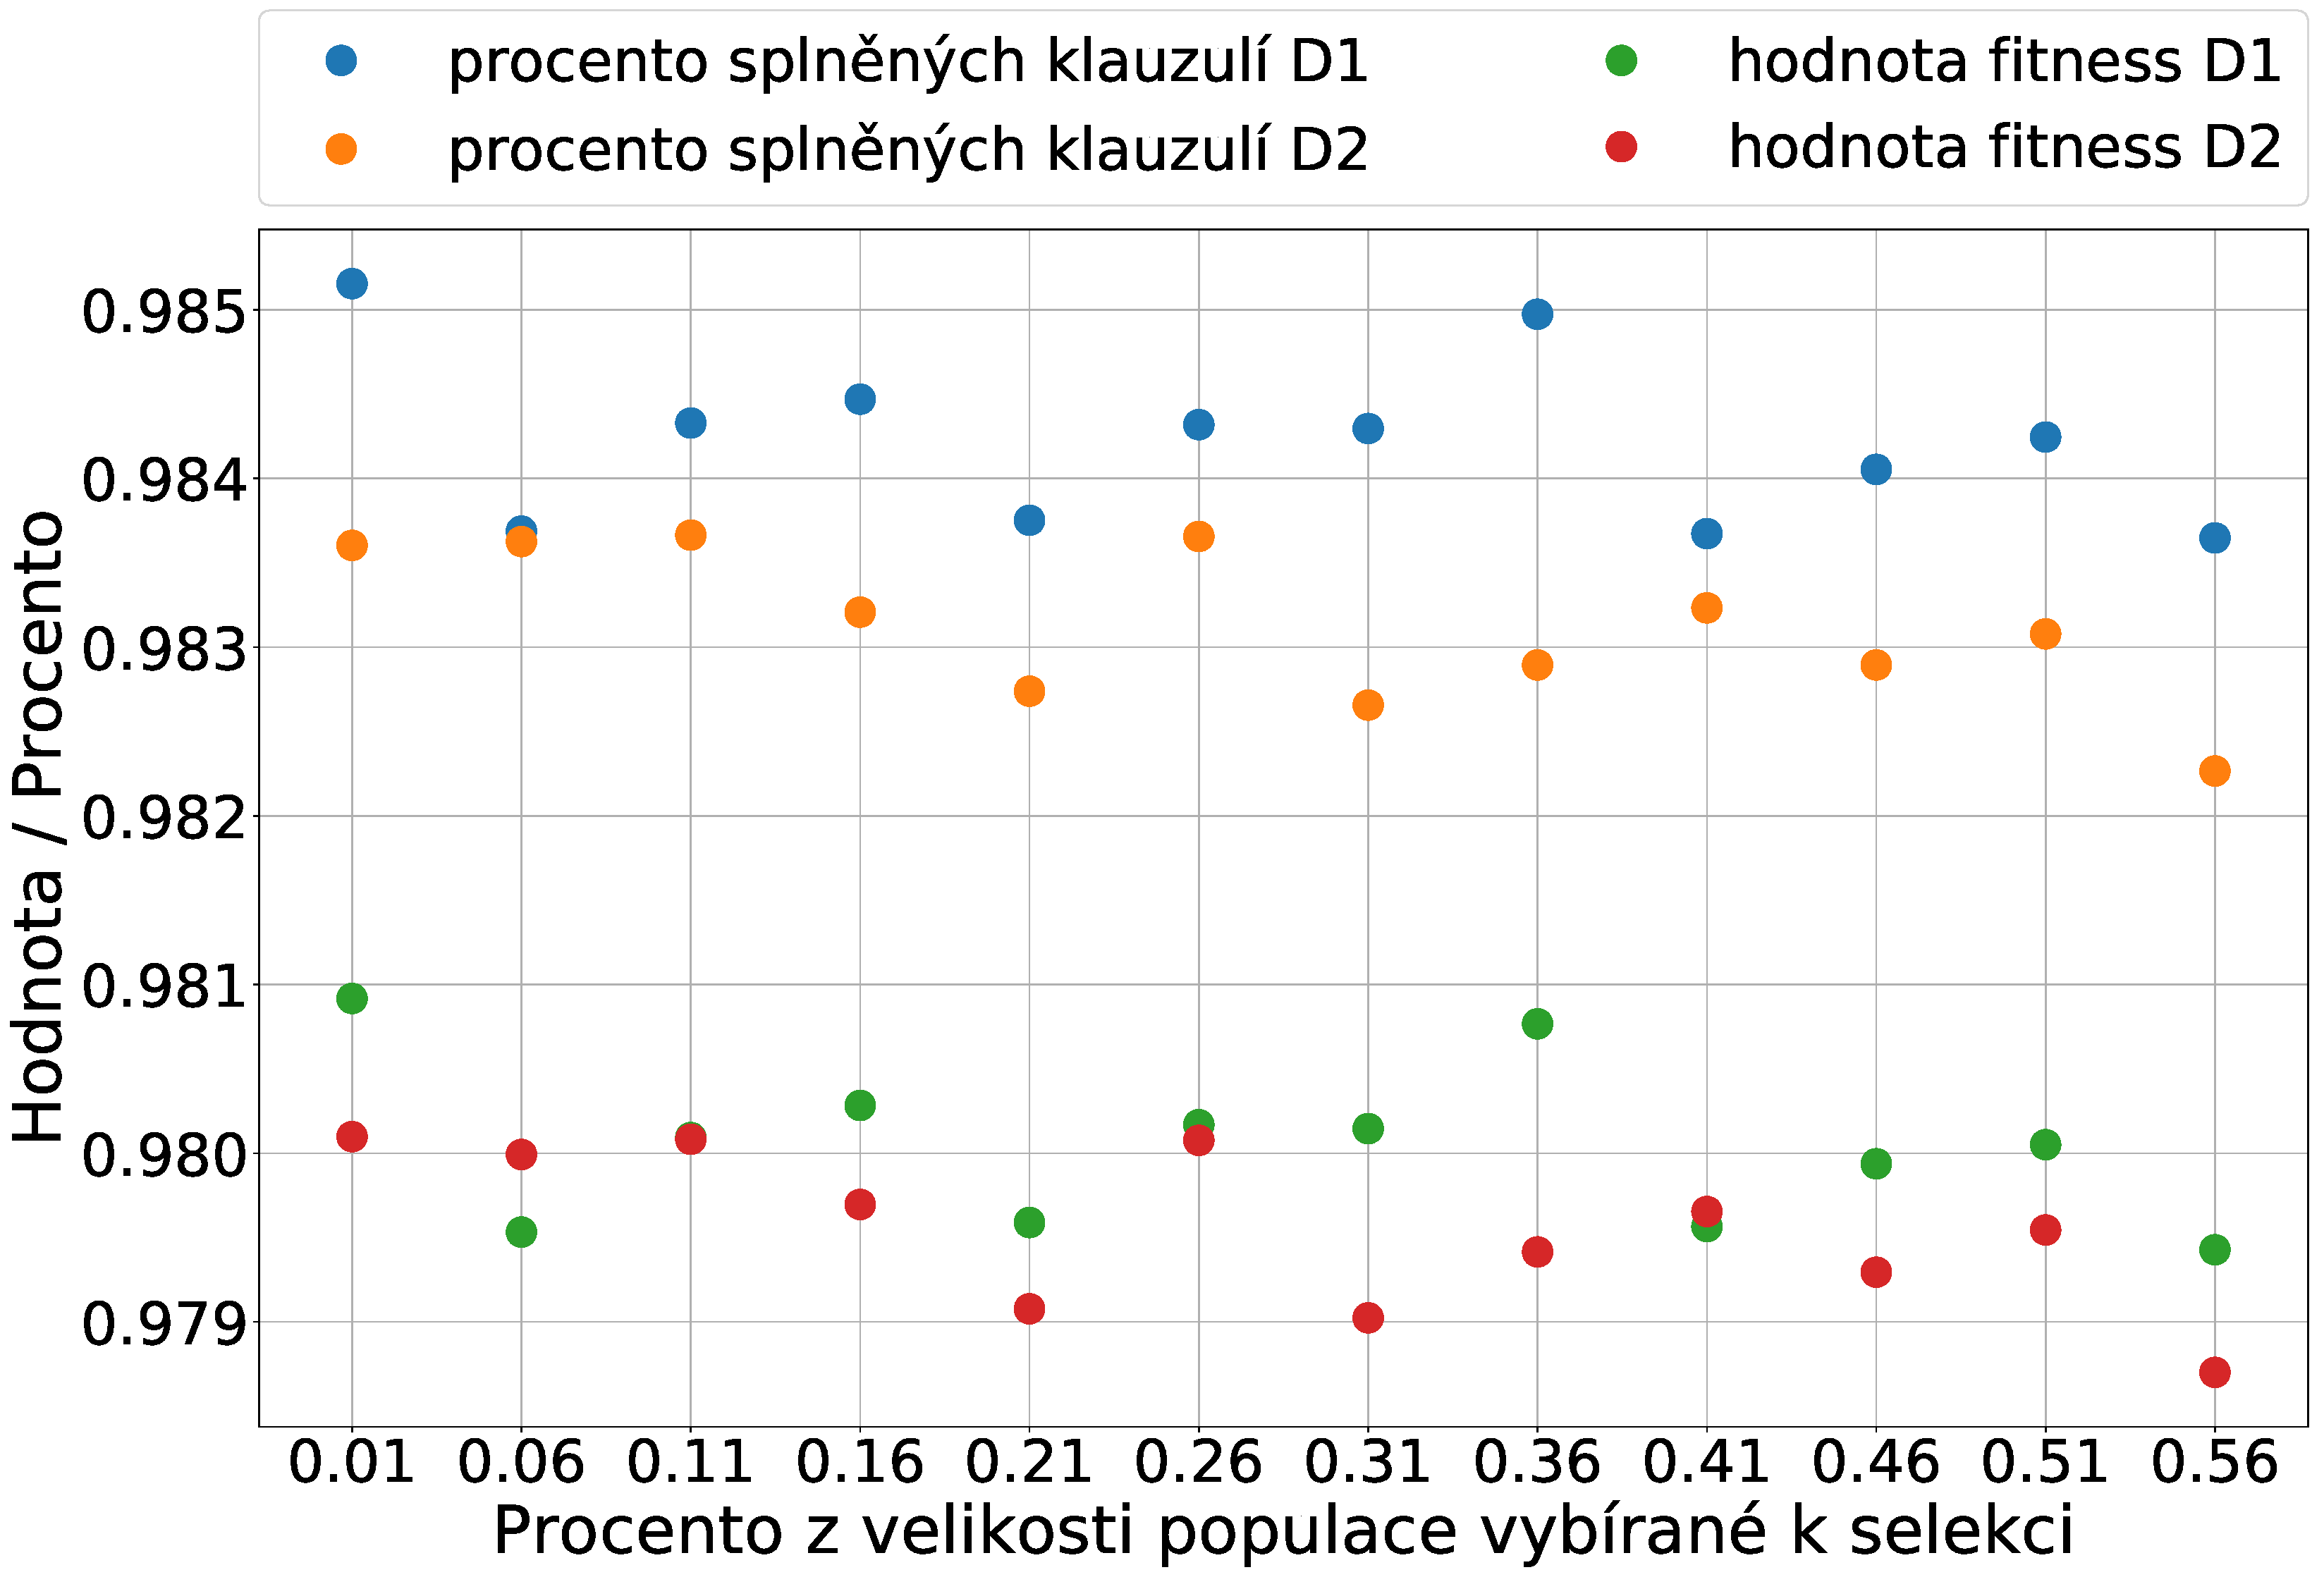
\includegraphics[width=\textwidth]{img/sat_s_small.pdf} 
    \end{minipage}
    \begin{minipage}[c]{0.48\textwidth}
        \centering 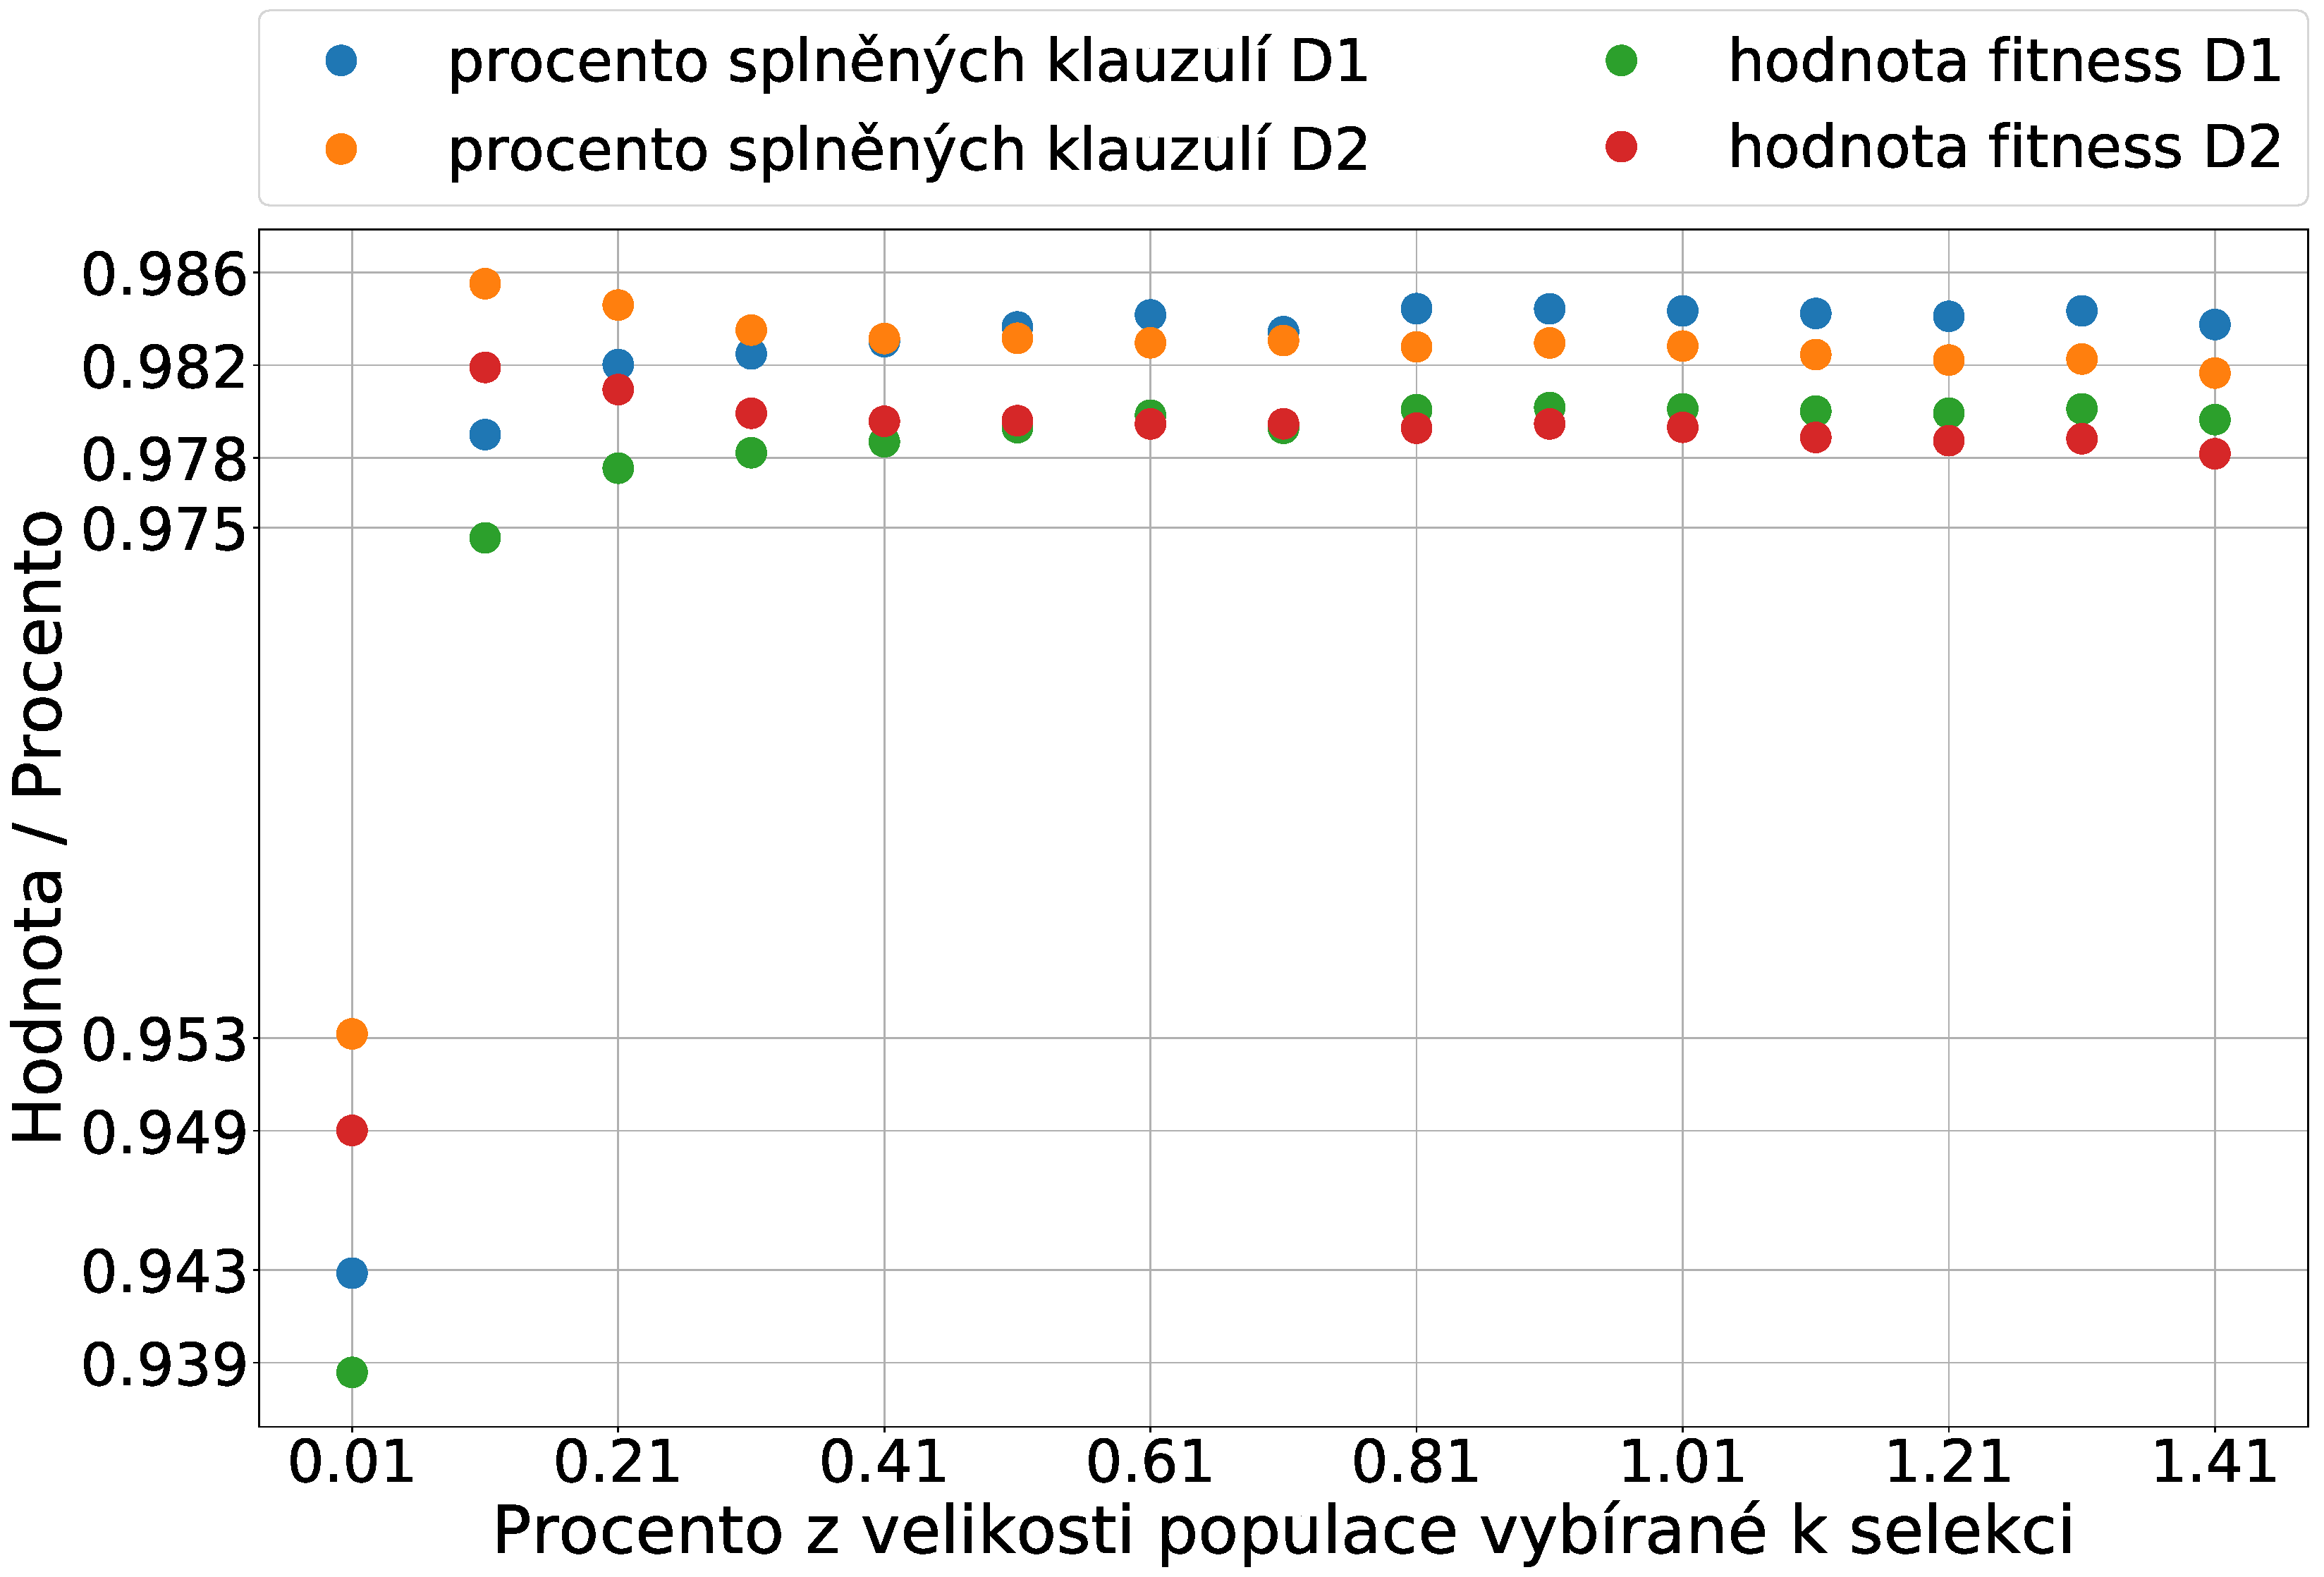
\includegraphics[width=\textwidth]{img/sat_s_big.pdf} 
    \end{minipage}
    \\
   \caption{Na grafech je vidět závislost úspěšnosti algoritmu na velikosti turnaje. Na obrázku vlevo je navíc zvyšující se velikost turnaje s každou generací o 2. Na pravém grafu toto použito není.}\label{fig:sel}
\end{figure} 

\subsection{Závislost na velikosti turnaje při selekci}
Další testovaný parametr byla selekce. V genetickém lgoritmu jsem implementoval turnojovou selekci. Selekční tlak je tedy řízen velikosti turnaje, kde malý turnaj dává velkou naději horším řešením z populace. Tento parametr je klíčový pro tzv. "tah na bránu", tedy aby algoritmus směřoval k~nějakému optimálnímu řešení, nejlépe tomu globalnímu. 

Na grafu \ref{fig:sel} je vidět úspěšnsnost na velikosti turnaje. Na levém grafu není patrný růst, ba naopak se zvyšující se mírou selekce, populace rychle konverguje. Toto je způsobeno zvyšujícím se selekčním tlakem, který i při nízkém nastavení rostl o konstantu a při způsobu testování, kde beru hodnotu fitness a procento splněných klauzulí se tento jev neprojeví. Tedy s narůstající hodnotou selekce je možné nastavit počáteční velikost selekce nízkou a tím dát algoritmu možnost prozkoumat větší část prostoru při přijímání horších řešení. 

Naopak na druhém grafu na obrázku \ref{fig:sel} je zobrazen vývoj selekce bez zvyšující se hodnoty. Zde jsou pro malou hodnotu patrné  horší výsledky, ale již pro 10 \% populace je hodnota selekce nejlepší pro náhodné problémy z datasetu D2. Pro dataset D1 je optimum až někde kolem 80 \% velikosti populace, tedy pro tyto data byl vhodnější vyšší selekční tlak. 80 \% však neznamená že půjde do turnaje 80 ze 100 jedinců. Jedinci jsou vybíráni náhodně s opakováním, takže se výsledný skutečný poměr může lišit.

Po testech bych jako optimální selekční tlak zvolil okolo 10 \% a s postupným zvyšování selekčního tlaku, tak jak jsem tyto parametry odhadnul na začátku. 

Na grafu \ref{fig:selrun} jsem ještě zobrazil ukázky z běhu, kde na levém obrázku je běh s nedostatečným selekčním tlakem, algoritmus tedy vůbec nekonverguje. Na pravém obrázku je graf s 10 \% selekcí bez zvyšování selekčního tlaku. 

\begin{figure}
	\centering
    \begin{minipage}[c]{0.48\textwidth}
        \centering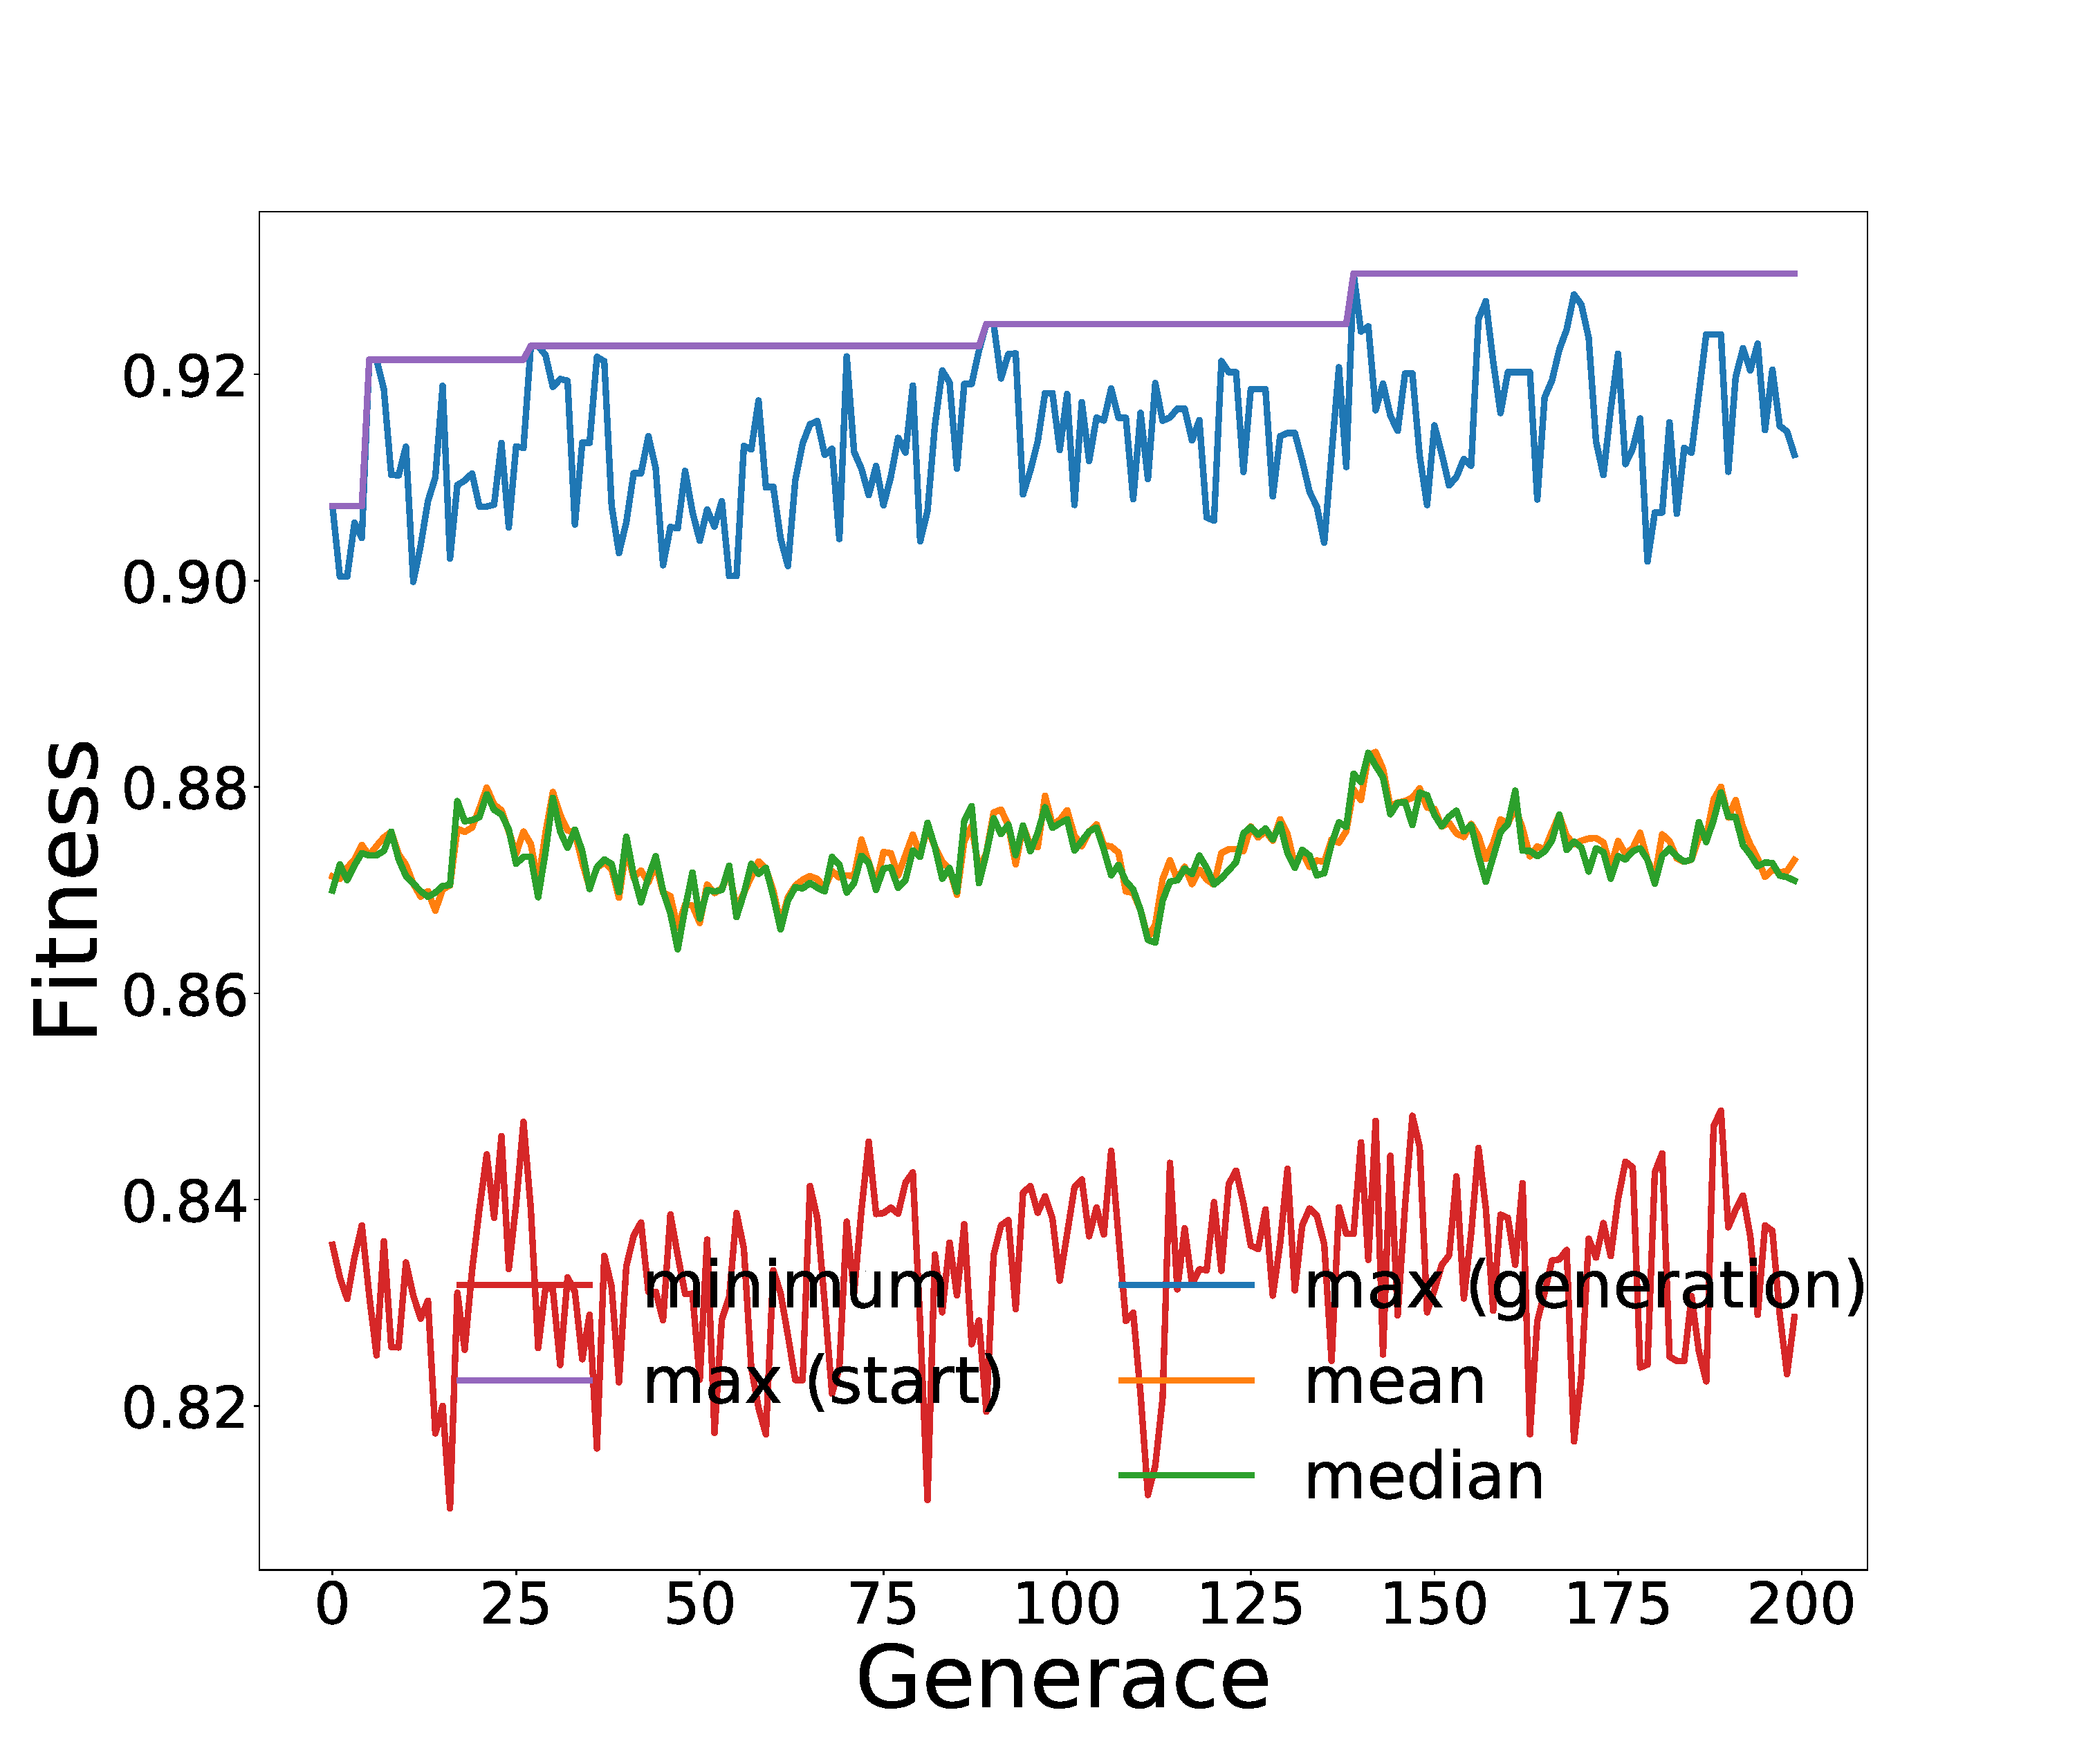
\includegraphics[width=\textwidth]{img/s_big_bad.pdf} 
    \end{minipage}
    \begin{minipage}[c]{0.48\textwidth}
        \centering 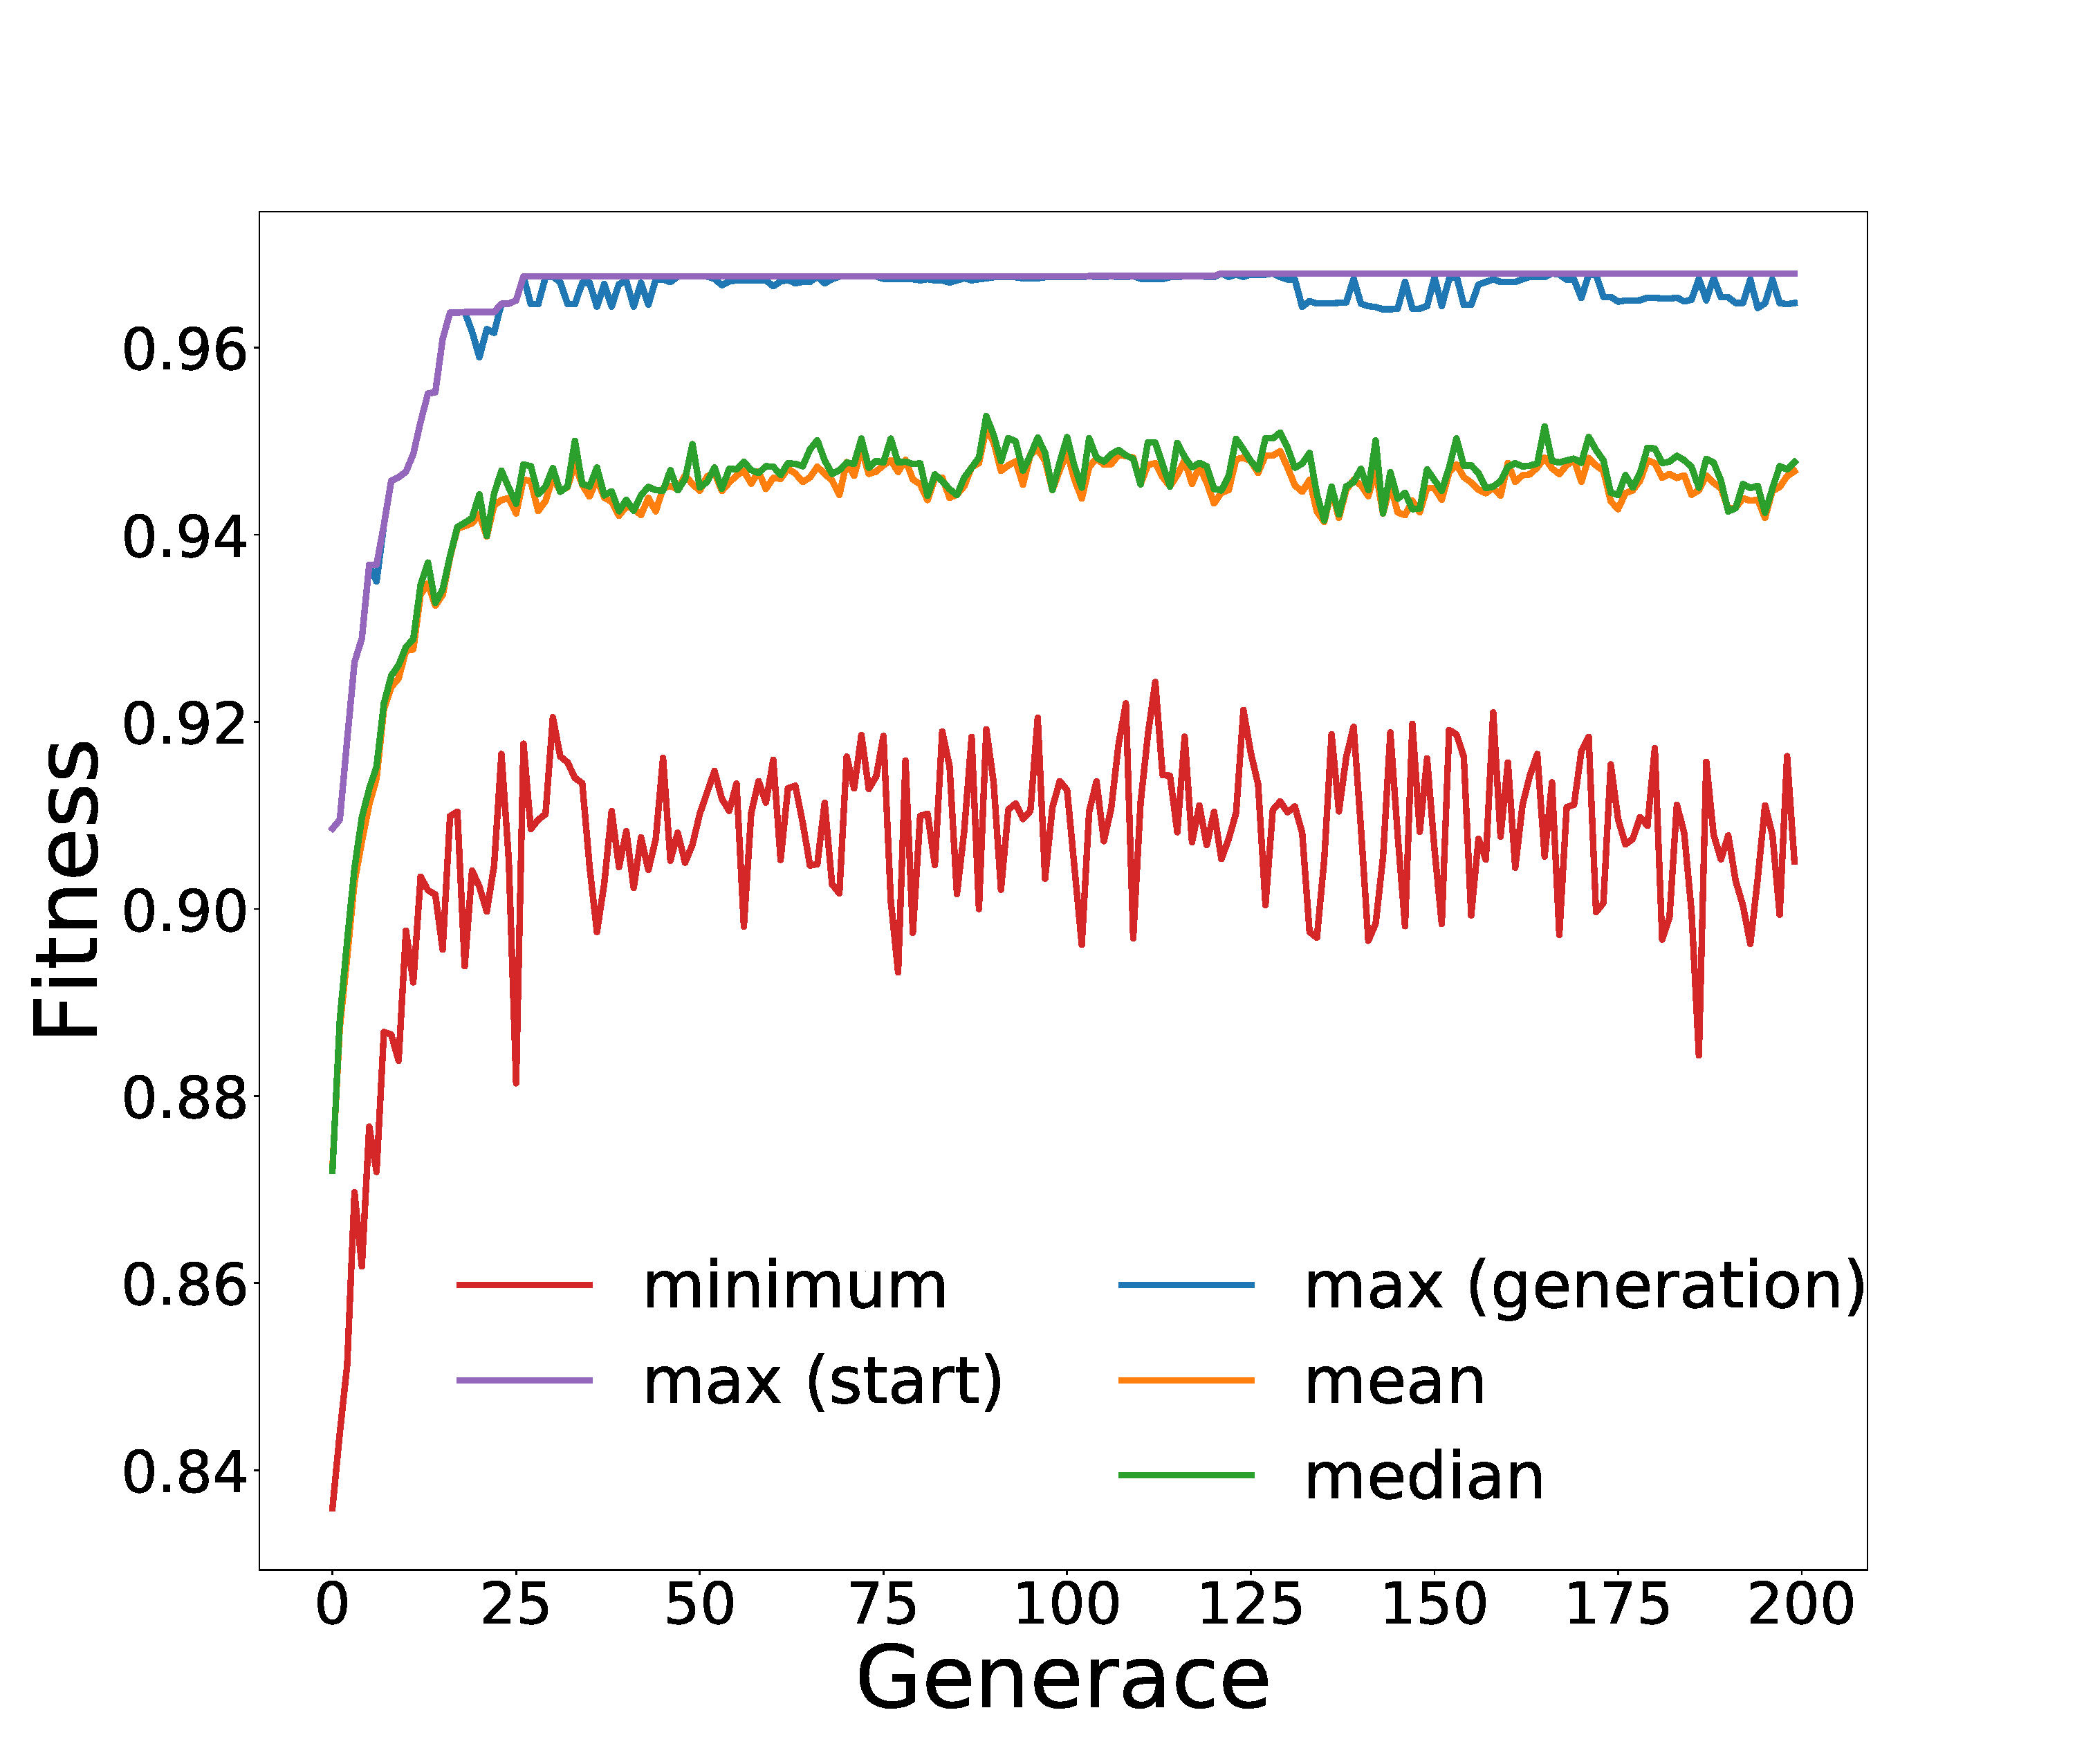
\includegraphics[width=\textwidth]{img/s_big_better.pdf} 
    \end{minipage}
    \\
   \caption{Na grafech je vidět průběh populace s rozdílnou hodnotou selekčního tlaku.}\label{fig:selrun}
\end{figure} 





\begin{wrapfigure}{r}{0.55\textwidth}
\begin{center}
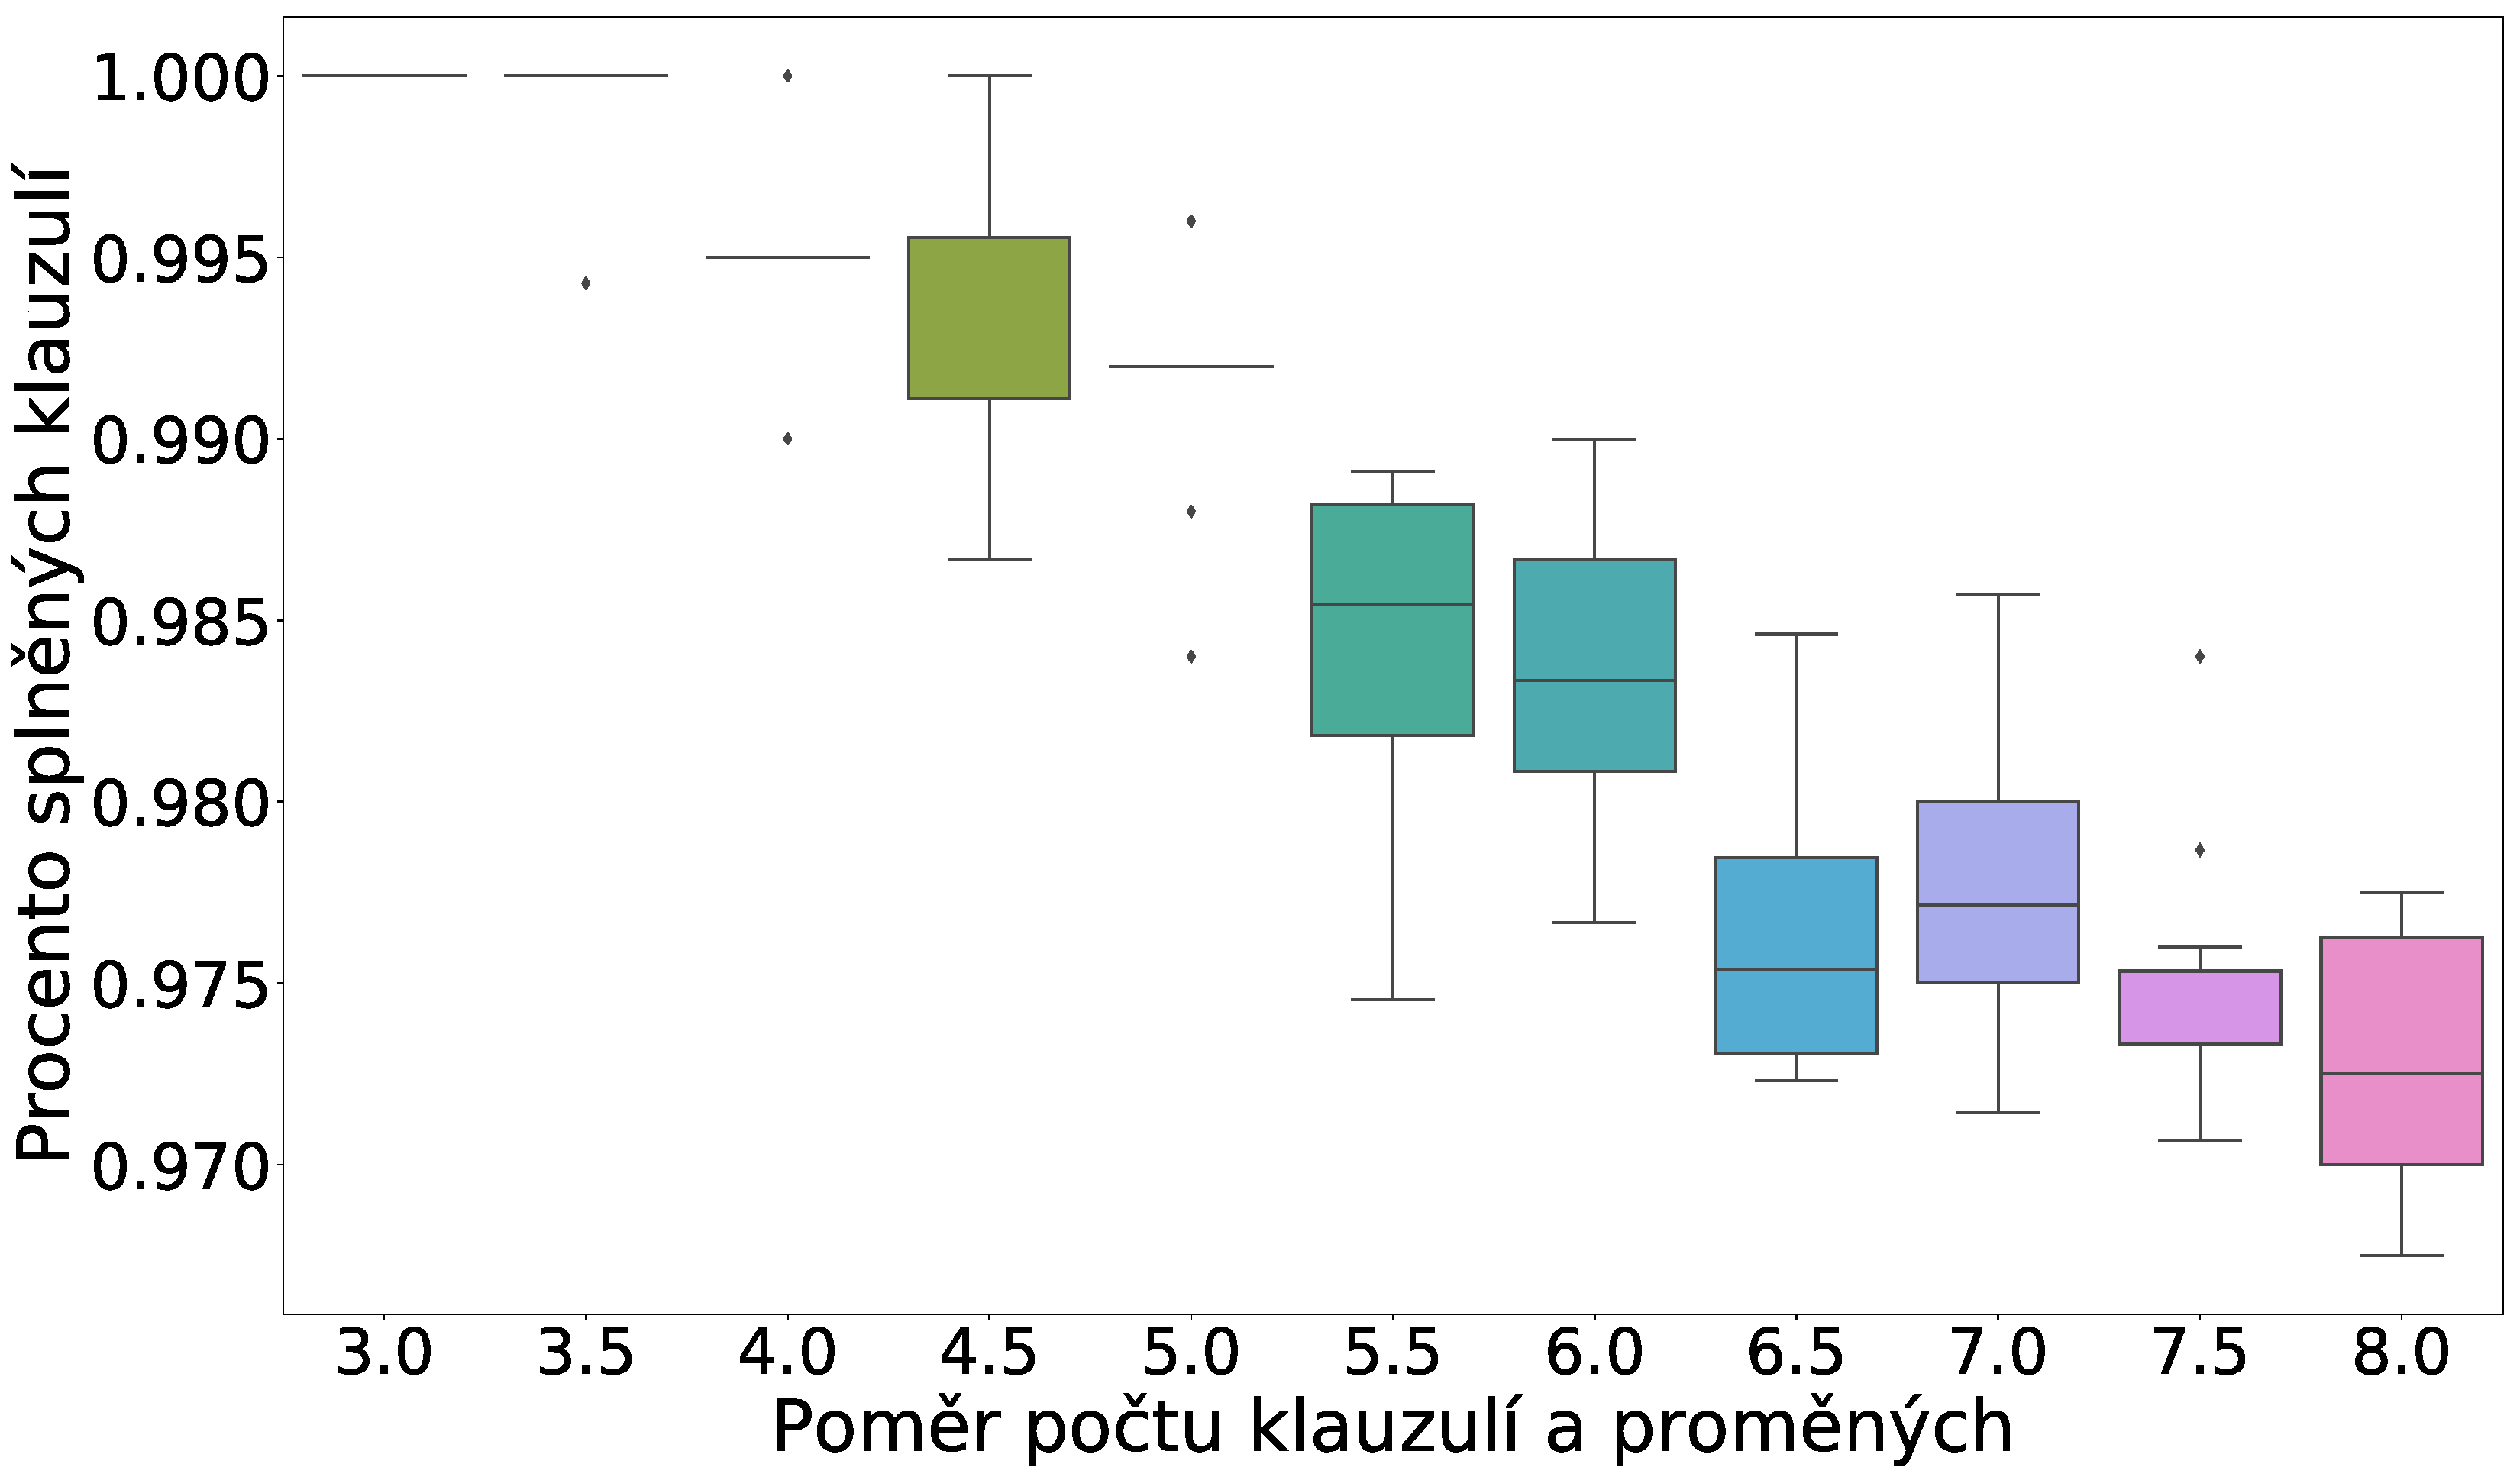
\includegraphics[width=0.55\textwidth]{img/boxRatio.pdf} 
\caption{Na obrázku je graf, kde je zobrazena úspěšnost v závislosti poměru počtu klauzulí na počtu proměných.}
\label{fig:box}
\end{center}
\end{wrapfigure}

\pagebreak

\subsection{Závislost na na poměru počtu klauzulí k počtu poroměných}
Na závěr jsem nastavil parametry a pokusil se změřit zdali je genetický algoritmus citlivý na poměr klauzulí a počtu proměných, při náhodně generovaných problémech a~u~váženého splnitelnosti booleovské formule.

Na obrázku \ref{fig:box} tato závislost není patrná. Spíše je patrná závislost na počtu klauzulí, protože testovací dataset má fixní počet proměných a jen je zvyšován počet klauzulí. Pro nízký poměr jsou klauzule jednoduší a téměř všechny byli vyřešeny a byly optimalizovány váhy. Se zvyšujícím se poměrem náročnost stále stoupala a ani s vyšší poměrem nebyli problémy opět jednodušeji řešitelné. Toto je způsobeno nejspíš, protože se zde nachází více podmínek (klauzulí) a genetický algoritmus je randomizovaný a jen se snaží vylepšovat konfigurace (nějaké nastavení proměných).

Naopak součásti většiny standartních řešičů SAT, které jsou založeny na CDCL nebo i jednoduché lokální algoritmy jako GSAT a WALKSAT, využívají při běhu jednotkovou propagaci. Tedy pokud klauzule ještě není splněná, ale již zbývá poslední neohodnocený literál, tak je nutné ho ohodnotit pozitivně. Jednotková propagace je velice efektivní pokud je v problému mnoho omezení (mnoho klauzulí) tedy při vysokém poměru náročnost při využití jednotkové propagace může velmi rychle klesat, protože díky jednotkové propagaci se povede vyřešit velké množství klauzulí. (Algoritmy a metody GSAT, WALKSAT, CDCL probrány v rámci předmětu MI-UMI)

Náhodně vygenerováné testovací problémy z datasetu D2 by bylo třeba otestovat na nějakém SAT řešiči, zdali se v tomto datasetu tento jev vůbec vyskuje, neboť to je teoretický předpoklad. Dále by bylo nutné závislost genetického algoritmu na poměru mnohem více prozkoumat, aby jí bylo možné s jistoutou například vyvrátit. Tento experiment můžu vzít jako směr, který by bylo nutné dále a důkladně prozkoumat.

\section{Závěr}\label{kap:zaver}
Během experimentu jsem využil pokročilou iterativní heuristiku k řešení problému vážené splnitelnosti problému SAT. Jako pokročilou iterativní heuristiku k tomuto problému jsem zvolil genetický algoritmus. Při testu jsem si vytvořil některé předpoklady o parametrech a ty jsem se pokusil potvrdit experimenty. Testoval jsem vždy velký rozsah hodnot, abych prozkoumal chování heuristiky na tyto parametry. 

Pro řešení problému jsem se pokusil nalézt některé parametry, které se mohou blížit optimu na mnou zvolených problémech. Nejvíce se parametry musejí měnit v závislosti na velikosti instance, kde malé populace a malý počet generací mohou zbůsobit nedostatečnou iterativní sílu heuristiky. Dále mohou mít jiný optimální bod v případě mutace. Na druhou stranu operátor křížení a selekce lze nastavit docela univerzálně a u operátoru selekce především pokud je zvolena zvyšující se míra selekce. 

Při nastavování algoritmu mohou nejvíce pomoc grafy vývoje populace, protože na nich je možné vidět některé nemoci, které může algoritmus mít, například příliž rychlou konvergenci nebo úplnou divergenci populace. U problému SATu nebylo tak optížné udržet diverzifikouvanou populaci, ale i tak se jednotlivá řešení mohla pohybovat pouze okolo některého lokálního minima, do kterého algoritmus zkonvergoval. 

Genetický algoritmus je randomizovaný algoritmus na principu Monte Carlo metod. Tedy stanovený počet kroků, které proběhnou, i když se nemusí podařit najít optimum. Ovšem není nutné, aby byl vždy algoritmus implementován na konečný počet cyklů, ale například na nějaký počet generací, které proběhnou po nalezení řešení v případě tohoto problému. Dále jde algoritmus vylepšit například paralelizací, kde mohou být simulovány populace na různých ostrovech, které si jen občas vymění nějakou genetickou informaci (jedince). Nebo například restart při příliž rychlé konvergenci a nedosažení požadovaného zlepšení.

Myslím si, že tato iterativní heuristika má velikou sílu a problém se podařilo docela obstojně řešit. Samozřejmě velice záleží na nastavených parametrech, které ovšem byly v rámci připravených datových sad D1 a D2 popsaných v kapitole \ref{kap:data}, nalezeny a řešení testováno.

\end{document}